%-----------------------------------
%-----------------------------------
% Msc Dissertation / Phd Thesis Template - Minds Lab
% Based on Abntex2
% Updated: November, 2018
%-----------------------------------
%-----------------------------------

\documentclass[
	12pt,				
	openright,			
	twoside,			
	a4paper,
	%brazil, % Texts in pt-br
	english			
]{abntex2}

%-----------------------------------
% Basic packages
%-----------------------------------
\usepackage[T1]{fontenc}		% Font
%\usepackage{times}
\usepackage[utf8]{inputenc}		% Special pt-br characters
\usepackage{lastpage}			% Catalographic card
\usepackage{indentfirst}		% Indent 1st paragraph
\usepackage{color}				
\usepackage{graphicx}			
\usepackage{microtype} 			% Justify (left and right side) 
\usepackage{makeidx}            % Remissive Index

%-----------------------------------
% Additional packages
%-----------------------------------
\usepackage{amsmath,amsfonts,amssymb}
\usepackage[table]{xcolor}
\usepackage{multirow}           % Merge rows and columns in tables
\usepackage{longtable}          % Large tables
\usepackage{fancyvrb}           % Codes and Outputs commands
\usepackage{listings}           % Codes and Outputs commands
\usepackage{pdflscape}
\usepackage{float}
\usepackage[authoryear]{natbib} % Authors imputation
\usepackage{subfig}             % Subfigures
\usepackage{latexsym}           % Extra symbols of Latex
\usepackage{booktabs}
\usepackage{enumerate}
\usepackage{acronym}
\usepackage{algorithm}          % Algorithms
%\usepackage[portuguese, ruled, linesnumbered]{algorithm2e} %to portuguese text, include this linha and comment the top row: \usepackage{algorithm}  
\usepackage[noend]{algpseudocode}
\usepackage{url}
%\let\realurl\url
%\renewcommand{\url}[1]{\realurl{#1}\wlog{URLX #1}}
\usepackage{rotating}
\usepackage{epigraph}
\usepackage{pbox}
\usepackage{subfig}
\usepackage{listings}
\usepackage{colortbl}
\usepackage{multirow}
\usepackage{array}
\usepackage{nameref}
\usepackage{psfrag}
\usepackage{epstopdf}
\usepackage{makeidx}
\usepackage{authorindex}
\usepackage{pdflscape}
\usepackage{fancyhdr,fancybox}
%\usepackage[algochapter,algoruled,linesnumbered,vlined]{algorithm2e}
\usepackage{graphicx}
\usepackage{latexsym}
\usepackage{amssymb,amsmath,amstext,amscd}
\usepackage{amsthm}
\usepackage{booktabs} 

%-----------------------------------
% Box the algorithm
\makeatletter
\def\BState{\State\hskip-\ALG@thistlm}
\makeatother

%-----------------------------------
% Front pages
%-----------------------------------
\titulo{Scalable Models for Probabilistic Forecasting with Fuzzy Time Series}
\autor{Petrônio Cândido de Lima e Silva}
\local{Belo Horizonte - Minas Gerais}
\data{July, 2019}
\orientador{Frederico Gadelha Guimarães}
\coorientador{Hossein Javedani Sadaei}
\instituicao{%
 	Federal University of Minas Gerais - UFMG
 	\par  
 	Graduate Program in Electrical Engineering - PPGEE
	\par 
	Machine Intelligence and Data Science Laboratory - MINDS
}

\tipotrabalho{Thesis (Doctorate)}
%\preambulo{Tese de Doutorado submetida à Banca	Examinadora 
% designada pelo Colegiado do Programa de Pós-Graduação em Engenharia Elétrica
% da Escola de Engenharia da Universidade Federal de Minas Gerais, como
% requisito para obtenção do Título de Doutor em Engenharia Elétrica.} 
\preambulo{Final thesis presented to the Graduate Program in Electrical Engineering  of  the  Federal  University  of  Minas  Gerais  in partial  fulfillment  of  the  requirements  for  the  degree  of Doctor in Electrical Engineering.}

%-----------------------------------
% Set the final PDF
%-----------------------------------
\definecolor{blue}{RGB}{41,5,195} % setting the blue color

% PDF informations
\makeatletter                   
\hypersetup{
     	%pagebackref=true,
		pdftitle={\@title}, 
		pdfauthor={\@author},
    	pdfsubject={\imprimirpreambulo},
	    pdfcreator={LaTeX with abnTeX2},
		pdfkeywords={abnt}{latex}{abntex}{abntex2}{trabalho acadêmico}, 
		colorlinks=true,        % false: boxed links; true: colored links
    	linkcolor=blue,         % color of internal links
    	citecolor=blue,        	% color of links to bibliography
    	filecolor=magenta,      % color of file links
		urlcolor=blue,
		bookmarksdepth=4
}
\makeatother

%-----------------------------------
% Spacing between lines and paragraphs
%-----------------------------------
\setlength{\parindent}{1.5cm}   % Set length of indent
\setlength{\parskip}{0.2cm}     % Set length among the paragraphs 

%Index
\makeindex

\setlength\epigraphwidth{.8\textwidth}
\setlength\epigraphrule{0pt}
\renewcommand{\epigraphflush}{flushleft}
\renewcommand{\sourceflush}{flushleft}

\newcommand{\newepigraph}[2]{\epigraph{\itshape ``#1''}{\hspace{5 mm}--- #2}}

%-----------------------------------
% Main document
%-----------------------------------
\begin{document}

\newcommand{\var}{\mathcal{V}}
\newcommand{\vari}{\mathcal{V}_i}
\newcommand{\ulvar}{\tilde{A}}
\newcommand{\mlvar}{\widetilde{\mathcal{V}}_i}
\newcommand{\tlvar}{\widetilde{*\mathcal{V}}}
\newcommand{\ufset}{A_j}
\newcommand{\mfset}{A_j^{\vari}}
\newcommand{\tfset}{A_j^{*\var}}
\newcommand{\model}{\mathcal{M}}
\newcommand{\estimate}{\hat{y}(t+1)}
\newcommand{\intvl}{\mathbb{I}}
\newcommand{\interval}{\intvl = [\underline{l},\overline{u}{]}}
\newcommand{\ifts}{[\mathbb{I}]FTS}
\newcommand{\FIG}{\mathcal{FIG}}
\newcommand{\fig}{\mathcal{G}}
\newcommand{\figi}{\mathcal{G}_i}
\renewcommand{\textdegree}{$^{\circ}$}



%-----------------------------------
%Language
%\selectlanguage{brazil}        % Texts in pt-br
\selectlanguage{english} 
\frenchspacing                  % Remove obsolete spaces between phrases

%-----------------------------------
% Pre-textual elements
\pretextual

%-----------------------------------
% Cover
\imprimircapa                   

% Folha de rosto
\imprimirfolhaderosto* % (o * indica que haverá a ficha bibliográfica)



%%-----------------------------------
% Cataloguing data

% Manually
% \begin{fichacatalografica}
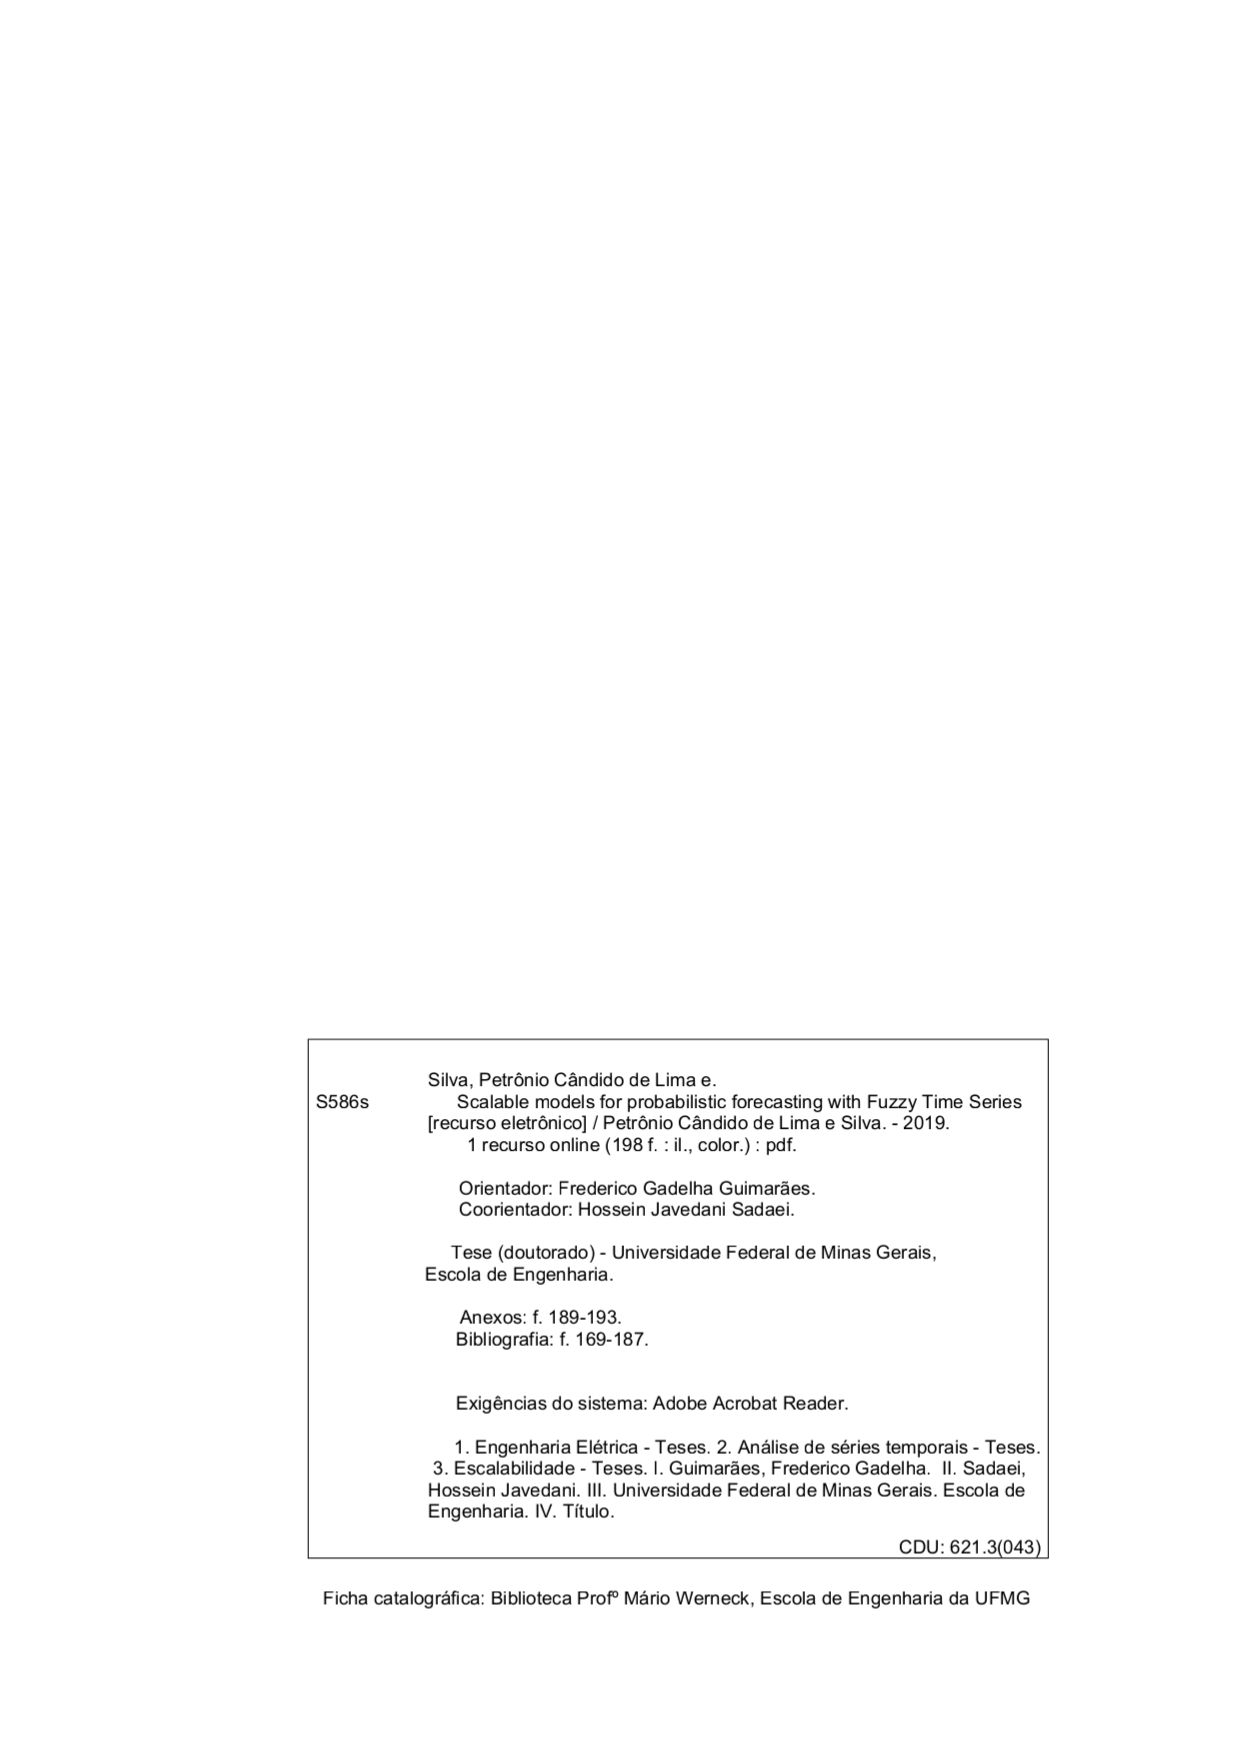
\includepdf{pre_textuals/ficha_catalografica.pdf}
% \end{fichacatalografica}

% or
% Automatically



\newpage

%-----------------------------------
% Dedication 
\begin{dedicatoria}
   \vspace*{\fill}
   \centering
   \noindent
   \textit{We all are the sum of many people - the result of their direct or indirect  efforts for us. We have no merit alone neither did nothing in our life by ourselves. Because this I dedicate this work to the wide web of people that somehow helped me to become what I am. When I remember the people around me in my life, with varying degrees of closeness, I realize that it is almost impossible to separate what is my own and what is influence absorbed from others. Because of this, I am continuously meditating about all my ancestors (also my parents in law) and my friends. It's always on my mind their disposition to help and their sacrifices to offer better life conditions to their sons, actions that paved the road I'm walking now. I'm grateful to all of you!} 
   \vspace*{\fill}
\end{dedicatoria}

%-----------------------------------
% Acknowledgments
\begin{agradecimentos}
I would like to thank all my familly, but at first place my parents Joaquim Cândido and Édina Lúcia that are the main responsible for this achievement.  You have no idea the respect, admiration and love I have for you. You are my heros! Also my parents in law, Antônio and Arlete, precious gifts that life gave me that I keep inside my heart. 

My grandfathers Olavo Cândido and Otávio Perpétuo and my grandmothers Maria da Conceição (Lia) and Maria Salomé (Nina), \textit{in memoriam}.

My precious jewel of light, my wife Nikaelle Fraga, I'm really devoted to you! You suffer with me each step of this odyssey, each pain and each victory. You deserve more credits for this than me, for having supported me and encouraged me to follow my dreams. You give meaning to my favorite quote: \textit{Ubi thesaurus tuus est, ibi cor tuum est}. I love you!

My brothers André and Ivana, my best friends since ever and forever and people that always inspired me. All my uncles and cousins that I will not nominate to avoid any omission, also my sister-in-law Ingrid and my godchildren João Rafael and Antônio Nicolau. 

My advisor Prof. Dr. Frederico Gadelha Guimarães, the best advisor ever and really a gifted person. I'm really proud to be your student and it's a honor to have the opportunity to learn with you! Best wishes also for his wife Rúbia Pereira and his lovely daughter Laura.

My co-advisor Prof. Dr. Hossein Javedani Sadaei, a fantastic person which to a person who helped me and taught me a lot, also possibly the world's greatest specialist on Fuzzy Time Series. It's a privilege to count on you!

My lifelong best friends Prof. Dr. Gefter Thiago, Prof. Dr. Márcio Ramos (Bisa) and Prof. Rodrigo Carneiro Brandão. Even living so far and been so unplugged, my thoughts will always be with you! You are the best guys ever! 

All professors and staff of the PPGEE - UFMG and my teammates on MINDS - Machine Intelligence and Data Science Laboratory, very special and careful people! Marcos Alves, Carlos Severiano, Gustavo Vieira, Tamires Rezende, Rodrigo Pedrosa, Cristiano Leite, Ivan Reinaldo, Rúbia Reis, Leonardo Augusto,  Giulia Zanon, Maria Victória, Fernando Galindres, Roozbeh, Kossar, Omid Orang, Babak and Bruno Alberto. Thank you very much!  

All colleagues and students of IFNMG - Instituto Federal do Norte de Minas Gerais. I will not nominate to avoid any  omission, except for these special guys: Paulo Vitor (PV),  Felipe (Bolinha) and Patrícia Lucas, my colleagues at PPGEE.

Finally, my kittens Perrengo, Yôda, Salém and Vingador, my companies during the long nights writing this work. Meow!

\vspace{5cm}


\begin{center}
\textbf{\textit{Glória in Excélsis Deo!}}
\end{center}

\end{agradecimentos}

%-----------------------------------
% Epigraph
\begin{epigrafe}
    \vspace*{\fill}
	\begin{flushright}
		\textit{
		"Simplicity is a great virtue but it requires hard work to achieve it and education to appreciate it. And to make matters worse: complexity sells better" (Edsger Wybe Dijkstra)}
	\end{flushright}
\end{epigrafe}

%-----------------------------------
% Resumo (abstract in Portuguese)
%\setlength{\absparsep}{18pt} % set spacing between the paragraphs

\begin{resumo}[Resumo]

No campo da previsão de séries temporais os métodos mais difundidos baseiam-se em predição por ponto. Esse tipo de previsão, no entanto, tem um sério inconveniente: ele não quantifica as incertezas inerentes aos processos naturais e sociais nem outras incertezas decorrentes da captura e processamento dos dados. Por isso nos últimos anos os métodos de previsão intervalar e probabilística têm ganhado a atenção dos pesquisadores, particularmente nas ciências climáticas e na econometria. Mas outro inconveniente vem do fato de grande parte dos métodos de previsão probabilística serem métodos de caixa preta e demandarem simulações estocásticas ou \textit{ensembles} de métodos preditivos que são computacionalmente despendiosos.

Por outro lado, o volume (número de registros) e a dimensionalidade (número de variáveis) dos dados vêm alcançando magnitudes cada vez maiores, graças ao barateamento dos dispositivos computacionais de captura e armazenamento de dados, um fenômeno conhecido como \textit{Big Data}. Tais fatores impactam diretamente no custo de treinamento e atualização dos modelos e, para séries temporais com essas características, a escalabilidade tornou-se um fator decisivo na escolha dos métodos preditivos.

Nesse contexto emergem os métodos de Séries Temporais Nebulosas, que vêm em crescente expansão nos últimos anos dado os seus resultados acurados, a facilidade de implementação dos métodos, o seu baixo custo computacional e a interpretabilidade de seus modelos. Os métodos de Séries Temporais Nebulosas têm sido utilizados em áreas como previsão de demanda energética, indicadores e ativos de mercado, turismo entre outras. Mas há lacunas na literatura de tais métodos referentes a escalabilidade para grandes volumes de dados e  previsão probabilística e por intervalos.

A presente tese propõe novos métodos escaláveis de Séries Temporais Nebulosas e investiga a aplicação desses modelos na previsão por ponto, intervalar e probabilística, para uma ou mais variáveis e para mais de um passo à frente. Os parâmetros e hiperparâmetros dos métodos são discutidos e são apresentadas alternativas de ajuste fino dos modelos. Os métodos propostos são então comparados com as principais técnicas de Séries Temporais Nebulosas e outros modelos estatísticos utilizando dados ambientais e do mercado de ações. Os modelos propostos apresentaram resultados promissores tanto nas previsões por ponto quanto nas previsões por intervalo e probabilísticas e com baixo custo computacional, tornando-os úteis para um vasta gama de aplicações.
        
Palavras-chave: Séries Temporais Nebulosas, Previsão Probabilística, Escalabilidade, Previsão por Intervalo.

\end{resumo}

%-----------------------------------
% Abstract (in English)
\begin{resumo}[Abstract]
    \begin{otherlanguage*}{english}

In the field of time series forecasting, the most known methods are based on point forecasting. However, this kind of forecasting has a serious drawback: it does not quantify the uncertainties inherent to natural and social processes neither other uncertainties caused by the data gathering and processing. Because this in last years the interval and probabilistic forecasting methods have been gaining more attention of researches, specially on environmental and economical sciences. But these techniques also have their own issues due to the methods being black-boxes and requiring stochastic simulations and ensembles of multiple forecasting methods which are computationally expensive.

On the other hand, the data volume (number of instances) and dimensionality (number of variables) have reached magnitudes even greater, due to the commoditizing of the capturing and storing computational devices, in a phenomenon known as Big Data. Such factors impact directly on the model's training and updating costs, and for time series with Big Data characteristics, the scalability became a decisive factor in the choosing of predictive methods.

In this context the Fuzzy Time Series (FTS) methods emerge, which have been growing in recent years due to their accurate results, easiness of implementation, low computational cost and model explainability. The Fuzzy Time Series methods have been applied to forecast electric load, market assets, economical indicators, tourism demand etc. But there is a lack on FTS literature regarding interval and probabilistic forecasting.

This thesis proposes new scalable Fuzzy Time Series methods and discusses its application to  point, interval and probabilistic forecasting of mono and multivariate time series, for one to many steps ahead. The parameters and hyper-parameters are discussed and fine tunning alternatives are presented. Finally the proposed methods are compared with the main Fuzzy Time Series techniques and other literature approaches using environmental and stock market data. The proposed methods obtained promising results on point, interval and probabilistic forecasting and presented low computational cost, making it useful for a wide range of applications.

\textit{Keywords: Fuzzy Time Series, Probabilistic Forecasting, Interval Forecasting, Scalable Models.}
    \end{otherlanguage*}
\end{resumo}

%-----------------------------------
% Preface
% Prefácio
\chapter*[Preface]{Preface} \index{Preface}

\newepigraph{From my part I know nothing with any certainty, but the sight of the stars makes me dream.}
{Vincent Van Gogh}

When Prof. Fred suggested me to study Fuzzy Time Series - I need to confess - I became excited. Because one of most fascinating issues on scientific research is to deal with uncertainty. Uncertainty is pervasive, omnipresent and self propagated. Pliny the Elder, early on first century of Cristian Age, stated that ``the only certainty is the uncertainty''. The mankind expanded the boundaries of the knowledge and some uncertainties could be reduced or eliminated. Others, however, remain irreducible. And here we are!

I always felt uncomfortable with the mechanistic and deterministic view of the world. The advances of science have forced us to assume some limitations of our knowledge and accept the separation between our known-knowns, the known-unknowns and even of the unknown-unknowns. We know now that we live in a fuzzy and probabilistic world. 

And until here we just talked about the present and the past. Things get even more interesting when we try to look ahead and predict the future. If we can't measure accurately some natural, social and economical processes, due to instrumentation limitations for example, and these processes are also  intrinsically non-deterministic, these uncertainties combined make the forecasting task complex and barely precise.

The fog of uncertainty becomes yet more dense as the forecasting horizon goes away: the forecasting methods needs to take account of all uncertainties on present to forecast ranges of possibilities on future. When we look more than one step in the future the forecasting method should consider all possible combinations in the range of variation of each past step - and this increases the complexity and the output uncertainty.

With this research problem in hand, many ideas on our mind, and a lot of excitement, we expect to give some contributions to this field. We focused on non-deterministic processes and assume that all measurements are not completely accurate, every single value actually represents a fuzzy neighborhood. We propose to bring the fuzzy time series to the domain of probabilistic forecasting. 

I hope you enjoy this work as I enjoyed to dreaming and implementing it. 



%-----------------------------------
% Figures list
\pdfbookmark[0]{\listfigurename}{lof}
\listoffigures*
\cleardoublepage

%-----------------------------------
% Tables list
\pdfbookmark[0]{\listtablename}{lot}
\listoftables*
\cleardoublepage

%-----------------------------------
% Algorithms list
%\pdfbookmark[0]{\listtablename}{loa}
%\listofalgorithms
%\cleardoublepage

%-----------------------------------
% Abbreviations
%-----------------------------------
% Abbreviations and acronyms
%-----------------------------------

\begin{siglas}
\item[ARIMA] Autoregressive Integrated Moving Average
\item[BSTS] Bayesian Structural Time Series
\item[CRPS] Continuous Ranked Probability Score
\item[DEHO] Distributed Evolutionary Hyperparameter Optimization
\item[FLR] Fuzzy Logical Relationship
\item[FLRG] Fuzzy Logical Relationship Group
\item[FTS] Fuzzy Time Series
\item[HOFTS] High Order Fuzzy Tine Series
\item[IFTS] Interval Fuzzy Tine Series
\item[LHS] Left Hand Side
\item[MAE] Mean Absolute Error
\item[MAPE] Mean Average Percent Error
\item[MVFTS] Multivariate Fuzzy Tine Series
\item[PWFTS] Probabilistic Weighted Fuzzy Tine Series
\item[QAR] Quantile Autoregression
\item[RHS] Left Hand Side
\item[RMSE] Root Mean Squared Error
\item[UoD] Universe of Discourse
\item[WHOFTS] Weighted High Order Fuzzy Tine Series
\item[WIFTS] Weighted Interval Fuzzy Tine Series
\item[WMVFTS] Weighted Multivariate Fuzzy Tine Series
\end{siglas}
\cleardoublepage

%-----------------------------------
% Symbols
%-----------------------------------
% Symbols
%-----------------------------------

\begin{simbolos}

\item[$Y \in \mathbb{R}^n$]  the crisp time series data 
\item[$n = |\var|$] the number of variables of $Y$, univariate if $n=1$ or multivariate if $n > 1$
\item[$y(t) \in Y$] an individual instance of $Y$ on time $t$
\item[$F \in \ulvar$] Linguistic time series produced by $Y$ fuzzyfication 
\item[$f(t) \in F$] an individual instance of $F$ on time $t$, such that $f(t) = \{ \ufset\;|\; \mu_{\ufset}(y(t)) \geq \alpha\; \forall \ufset \in \ulvar \}$
\item[$U = [\underline{l},\overline{u}{]}$] the Universe of Discourse of a univariate $Y$, where the lower bound is $l = \min Y$ and the upper bound is $u = \max Y$.
\item[$T \in \mathbb{N}^+$] the total length of $Y$
\item[$t \in T$]  the time index
\item[$k \in \mathbb{N}^+$] the number of partitions of $U$
\item[$\alpha \in [0,1{]}$] the Alfa-Cut, the minimal membership grade to be considered in fuzzyfication process
\item[$\Omega \in \mathbb{N}^+$] the Model order, the number of time series lags used by model
\item[$L$] the lag indexes
\item[$\mu_{\ufset}: U \rightarrow [0,1{]}$] the fuzzy membership function for fuzzy set $\ufset$, $j = 1..k$ 
\item[$\ulvar$] the linguistic variable for univariate $Y$
\item[$\ufset \in \ulvar$] the individual fuzzy sets in $\ulvar$, $j = 1..k$
\item[$\var$] the set of variables of a multivariate $Y$
\item[$\vari \in \var$] an individual variable of $Y$, $i = 1..n$
\item[$*\var \in \var$] the target variable (or endogenous variable) of $Y$ 
\item[$U_i$]  the Universe of Discourse of each  $\vari$, for multivariate $Y$ , $i = 1..n$
\item[$k_i$] Number of partitions of $U_i$ for each  $\vari$, for multivariate $Y$, $i = 1..n$
\item[$\alpha_i$] Alpha-Cut for each $\vari \in \var$, $i = 1..n$
\item[$\mlvar$] the linguistic variable for each $\vari \in \var$, the group of fuzzy sets, $i = 1..n$
\item[$\mfset \in \mlvar$] the individuals fuzzy sets in $\mlvar$, $i = 1..n$ and $j = 1..k_i$
\item[$\model$] the FTS model, including the linguistic variable $\ulvar$ and the knowledge model
\item[$|\model|$] the model parsimony, the amount of parameters of the model
\item[$H \in \mathbb{N}^+$] The forecasting horizon, i.e, the number of steps to predict ahead
\item[$\estimate \in \mathbb{R}^n$] a point forecast for time $t+1$
\item[$\interval$] a prediction interval for time $t+1$ with lower bound $l \in \mathbb{R}$ and upper bound $u \in \mathbb{R}$
\item[$P: U \rightarrow [0,1{]}$] a probability distribution forecast for time $t+1$
\end{simbolos}
\cleardoublepage

%-----------------------------------
% Summary
\pdfbookmark[0]{\contentsname}{toc}
\tableofcontents*
\cleardoublepage


%-----------------------------------
% TEXTUAL ELEMENTS
%-----------------------------------
\textual

%-----------------------------------
% Chapters
\chapter[Introduction]{Introduction} 
\label{chap:Intro} \index{Introduction}

\newepigraph{In the strict formulation of the law of causality - if we know the present, we can calculate the future - it is not the conclusion that is wrong, but the premise.}
{Werner Heisenberg}

A significant part of scientific and engineering applications demand the forecasting of natural, social and economical processes and there are an extensive literature on forecasting methods and models. Such methods are also preceded by many  processes: instrumentation, measurement, storing, summarization, etc. However, a great recurrent problem is how to deal with the uncertainty generated or captured in each step of this task, and measure how it spreads. \cite{Makridakis2009} stated that ``Statistical models underestimate uncertainty, sometimes catastrophically'', by assuming, for example, that events are independent, forecasting errors are tractable, the variance of forecasting errors is finite, known and constant. 

\index{Ontological uncertainty}\index{Intrinsic uncertainty}\index{Irreducible uncertainty}

In these natural and social processes the uncertainty can be intrinsic or extrinsic and is classified, by \cite{Georgescu2014}, in two categories: the epistemic uncertainty and the ontological uncertainty. The ontological uncertainty represents the intrinsic and irreducible uncertainty of a process defined basically as the non-deterministic behavior - randomness and stochasticity - that usually is modeled by the probability theory. 

\index{Epistemic uncertainty}\index{Extrinsic uncertainty}\index{Reducible uncertainty}

On the other side, the epistemic uncertainty represents the extrinsic and reducible sources of uncertainty on a process like vagueness, lack of information and imprecision due to measurement errors, sensor calibration and other unknown factors. Another possibility is the conversion of continuous processes to discrete processes. This conversion is not lossless and some uncertainty is imputed on converted data. The epistemic uncertainty can be modeled by the fuzzy theory. 

This is the case of data preprocessing tasks, for example. Very often time series datasets need to be aggregated by some time resolution (daily, hourly, etc) and this aggregation also introduce the epistemic uncertainty on data. A good example are the financial markets time series that summarize all transactions of a whole day in four numbers: opening, minimum, maximum and closing prices. This method is an attempt to represent the volatility (e. g. the uncertainty) of the price value inside a certain time window and is also a tool for detecting patterns on data, the Candlestick Graph techniques, as shown in Figure \ref{fig:candlestick}. Sometimes the aggregation is even more aggressive and all the values are summarized in one, the average or median value, hiding all information about the volatility. When this data is used as input for fitting a forecasting model the extrinsic uncertainty is introduced.

\begin{figure}
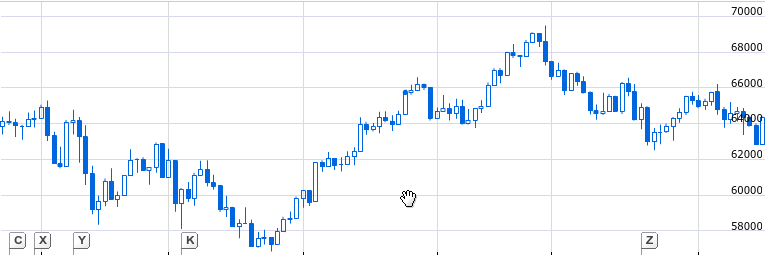
\includegraphics[width=\textwidth,height=2in]{figures/candlestick.png}
\caption[Candlestick chart for IBOVESPA]%
{Candlestick chart for IBOVESPA. Source: Google Finance\protect\footnotemark}
\label{fig:candlestick}
\end{figure}

\footnotetext{\url{https://www.google.com/financeq=INDEXBVMF\%3AIBOV&ei=zHz2WOmMKODrep_bgbAI}. Access in 18/04/2017}

The forecasting methods propagate the input uncertainties on their outputs and compromise the reliability of the forecast. Despite these points, the majority of forecasting methods are concerned with one step ahead point forecasting without output uncertainty measures. When the many steps ahead forecasting is considered, the uncertainty grows yet more and affects the accuracy and reliability of models. This effect becomes even worst  as the forecasting horizon becomes wider.

This fact led to the development of methods for Probabilistic Forecasting \cite{Gneiting2014b} and  Interval Forecasting \cite{Chatfield1993},  to deal with forecasting uncertainty by estimating distributions of possible values instead of a unique point forecast. The Interval Forecasting can be viewed as a particular case of the Probabilistic Forecasting where the probabilities are uniform inside the bounds of the interval forecast. However, traditional methods of probabilistic forecasting require the use of parametric models with distribution assumptions, as in Bayesian Inference, or costly estimation techniques and Monte-Carlo simulations. Probabilistic forecasting has been used in areas such as weather forecasting (\cite{Fraley2011} and \cite{Leutbecher2008}) eletric load forecasting (\cite{Hong2016}, \cite{Hong2016a} and \cite{Liu2015}), wind power generation (\cite{Pinson2006} and  \cite{Netto2016}) and hydrological forecasting (\cite{Laio2007}).

Side by side with the uncertainty representation in time series forecasts, some other factors became prevailing in the evaluation of predictive methods, such as Big Data scalability and model explainability. The Big Data phenomenon emerged in the late 2000s decade \cite{Lynch2008} calling attention to new demands on data analysis brought by the growth of data volume, dimensionality and variety. This revolution was possible due the advances on the technologies of data capturing and storage, as well its commoditizing, allowing the distributed management of amounts of data never seen before. 

But traditional forecasting methods, and even some newer ones, were not designed to deal with such high volume of data. The most critical issues were the high dimensionality  (dozens of hundreds of attributes) and volume (hundreds of millions or billions of samples) \cite{Qiu2016}. Such data volume cannot be grounded on a single machine memory and demands a distributed architecture of storage and processing. New technologies emerged to tackle these issues, for instance the Map Reduce based frameworks \cite{Dean2008}, a divide-and-conquer approach which is the basis of Hadoop clusters \cite{White2012}, where the processing units also act as storage units of the data subsets using commodity and cheap hardware assets.

The Big Data issues do not stop on data volume an, indeed, the velocity and variability of the data must be seriously considered when developing forecasting models. Many sources of data has non-stationary behaviors, meaning that they statistical properties may change along the time. Some models are time-variant, they are specially designed to be self-adaptable and evolve as the data changes. But the majority of the  conventional methods are time-invariant and need to be retrained periodically depending on the variability of the data, what can can be problematic given the computational cost of the training and adapting procedures. Yet more critical is the data with Concept Drifts \cite{} -, which have high volume with high velocity and need to be adaptable to new behaviors in feasible time. 

Another traditionally neglected aspect of the forecasting methods also started to gain more attention in recent years: the explainability. With the expansion of the machine learning methods enabled to tackle Big Data, another issues came up to the light: black-box methods started to find legal barriers or adoption resistance due to its lack of transparency and auditability. In other hand, the white-box methods can help in the knowledge extraction and simplification of complex temporal patterns, besides being easily auditable.

%If all these concerns (uncertainty representation,  scalability, low computational cost, explainability and self-adaptability) were taken in account, it becomes pretty hard to find a fitting method. But several of these issues
%the development of new soft-computing methods
The exposed scenario favored the rising of the Fuzzy Time Series (FTS) methods \cite{song1993fuzzy}, which have been drawing more  attention and relevance in recent years due to many studies reporting its good accuracy compared with other models \cite{Singh2008}. Fuzzy Time Series are soft-computing methods that produce data-driven, non-parametric, simple, computationally cheap and readable models for time series analysis and forecasting. FTS methods are also an approach to deal with  the  epistemic uncertainty, as on the time-aggregation case of the financial time series. The fuzzyfication of data gives a more flexible representation to the individual measures, embracing the range of possible value fluctuations not covered by the single values. 

Despite the great improvements published on FTS literature in the recent years, there are still some notable lacks. Interval and probabilistic forecasting, specially for many steps ahead, are not properly explored, besides the absence of scalable methods to tackle big multivariate time series. There is, indeed, a plethora of soft-computing forecasting methods. But very few of them are flexible enough to incorporate scalable point, interval, probabilistic and multivariate forecasting, with one to many steps ahead, for univariate and multivariate time series. This research opportunity is exploited in this work by the proposition of new FTS methods and their subsequent application on several case studies, including financial, environmental and energetic time series. 

\section{Objectives} \index{Objectives} 

\index{Probabilistic Weighted Fuzzy Time Series}\index{$\mathbb{P}W$FTS}
\index{Probabilistic Weighted Fuzzy Logical Relationship Groups}\index{PWFLRG}

The main goal of this thesis is to develop a scalable probabilistic forecasting approach based on the Fuzzy Time Series methods, providing a flexible computational framework for applications with uncertainties. Specific goals are divided in:

\begin{itemize}
\item Identify the strengths and weaknesses of the main FTS approaches presented in literature;
\item Identify extension opportunities on known probabilistic forecasting methods;
\item Introduce the Probabilistic Weighted Fuzzy Time Series, a new method family that exploits uncertainties on datasets to capture time series patterns and translate them into the rule-based knowledge system (the Probabilistic Weighted Fuzzy Logical Relationship Groups);
\item Improve PWFTS scalability in order to enable it to deal with big time series by proposing a distributed processing design with the Map/Reduce paradigm; 
\item Extend the PWFTS method to enable multivariate time series using Fuzzy Information Granules.
\end{itemize}

\section{Work structure} \index{Work structure}

This thesis is organized as follows:

\begin{itemize}
\item \textbf{Chapter \ref{chap:review_fts} - \nameref{chap:review_fts} } presents a contextual background on Fuzzy Time Series methods and discusses the most relevant methods in literature;

\item \textbf{Chapter \ref{chap:review_probforecasting} - \nameref{chap:review_probforecasting} } introduces the probabilistic forecasting concepts and main techniques, reviewing the surrounding literature. On section \ref{sec:ifts} is proposed the Interval Fuzzy Time Series method for binding the the fuzzy uncertainty on forecasts, and on section \ref{sec:ensemblefts} is proposed the EnsembleFTS method to probabilistic forecasting;

\item \textbf{Chapter \ref{chap:pwfts} - \nameref{chap:pwfts}} introduces the Probabilistic Fuzzy Time Series method for generating the Probabilistic Weighted Fuzzy Temporal Pattern rules and a method to generate one step ahead probabilistic forecasts; on section \ref{sec:pwfts_interval} the previous method is extended to create prediction intervals and on section \ref{sec:pwfts_point} is presented a simple heuristic to produce point forecasts. The section \ref{sec:pwfts_extensions} presents extensions for many steps ahead forecasting and high-order models. The characteristics and parameters of the methods are discussed in section \ref{sec:pwfts_experiments};

\item \textbf{Chapter \ref{chap:scalability} - \nameref{chap:scalability}} proposes a distributed approach for PWFTS, based on Map/Reduce paradigm and computational clusters, enabling it to deal with big time series. On section \ref{sec:hyperparameter} the Distributed Evolutionary Hyperparameter Optimization (DEHO) is proposed, employing evolutionary algorithms with the distributed processing to improve the performance.

\item \textbf{Chapter \ref{chap:multivariate} - \nameref{chap:multivariate}} proposes an extension for multivariate time series using Fuzzy Information Granules (FIG) and an incremental universe of discourse partitioner. With this extension PWFTS can be used for multivariate forecasting in a Multiple Input/Multiple Output (MIMO) design or singlevariate forecasting in a Multiple Input/Single Output(MISO) design.

%\item \textbf{Chapter \ref{chap:results} - \nameref{chap:results}} an empirical analysis is employed to validate the proposed method, using open datasets and standard measures, and to compare its performance with others well-known literature methods.

\item \textbf{Chapter \ref{chap:conclusions} - \nameref{chap:conclusions}} the findings are summarized and overall conclusions are given, as well as the contributions, known limitations and future investigations. 
\end{itemize}

\section{Main contributions} \index{Contributions}

This research present contributions to the Forecasting and Fuzzy Time Series research fields, whose the most important are summarized below:

\begin{itemize}
    \item development of the Probabilistic Weighted Fuzzy Time Series - PWFTS, which is a new non-parametric, data driven and highly accurate forecasting method, the first FTS method in the literature that integrates point, interval and probabilistic forecasting in the same model, for one to many steps ahead;
    \item a new representation method for fuzzy temporal rules, with weights on the precedent and the consequent of the rules, reflecting its \textit{a priori} and \textit{a posteriori} empirical probabilities and aid with model explainability;
    \item new defuzzyfication methods capable to produce probability distributions, prediction intervals and point forecasts and multivariate output using Fuzzy Information Granules (FIG);
    \item the pyFTS library \cite{pyFTS}\footnote{\url{http://pyfts.github.io/pyFTS/}} for Python programming language, an open and free framework to facilitate the development of new models and help on research reproducibility;  
    \item application of the proposed methods in the forecasting of renewable energy and environmental processes;
\end{itemize}



\chapter[Fuzzy Time Series]{Fuzzy Time Series} 
\index{Fuzzy Time Series}
\label{chap:review_fts}

\newepigraph{There's nothing worst than a sharp image of a fuzzy concept}{Ansel Adams}

This chapter aims to introduce the Fuzzy Time Series methods and review the relevant literature, offering a soft background on  the key concepts and models on this research field.

The name Fuzzy Time Series (FTS) can be used to refer to $F$, a time series composed by fuzzy linguistic terms, or the family of non-parametric forecasting methods introduced by \cite{song1993fuzzy} based on Fuzzy Set theory \cite{Zadeh1965}. These methods are easy to implement and very flexible, affording ways to  deal with numeric and non-numeric data.  FTS methods have been commonly employed in forecasting of university enrollments (\cite{song1993fuzzy}, \cite{Song1994}, \cite{ismail2011enrollment}), 
stock markets (\cite{Sadaei2016}, \cite{Lee2013},  \cite{chen2014high}, \cite{Sun2015}, \cite{Talarposhti2016a}, \cite{efendi2013improved}), 
tourism (\cite{Lee2011}), 
electric load (\cite{Ismail2015}, \cite{Sadaei2017}),  
seasonal time series [\cite{Song1999},  \cite{Chang1997}] among many others.
There are still some gaps in FTS methods (\cite{Sadaei2013} and \cite{Georgescu2010}) related with methodological problems but many of them have been approached in more recent studies \cite{JavedaniSadaei2016c}. There are several categories of FTS methods whose main features and its variations can be seen in Figure \ref{fig:fts_taxonomy}, and will be discussed in the remaining sections.  

\begin{figure}[htb]
    \centering
    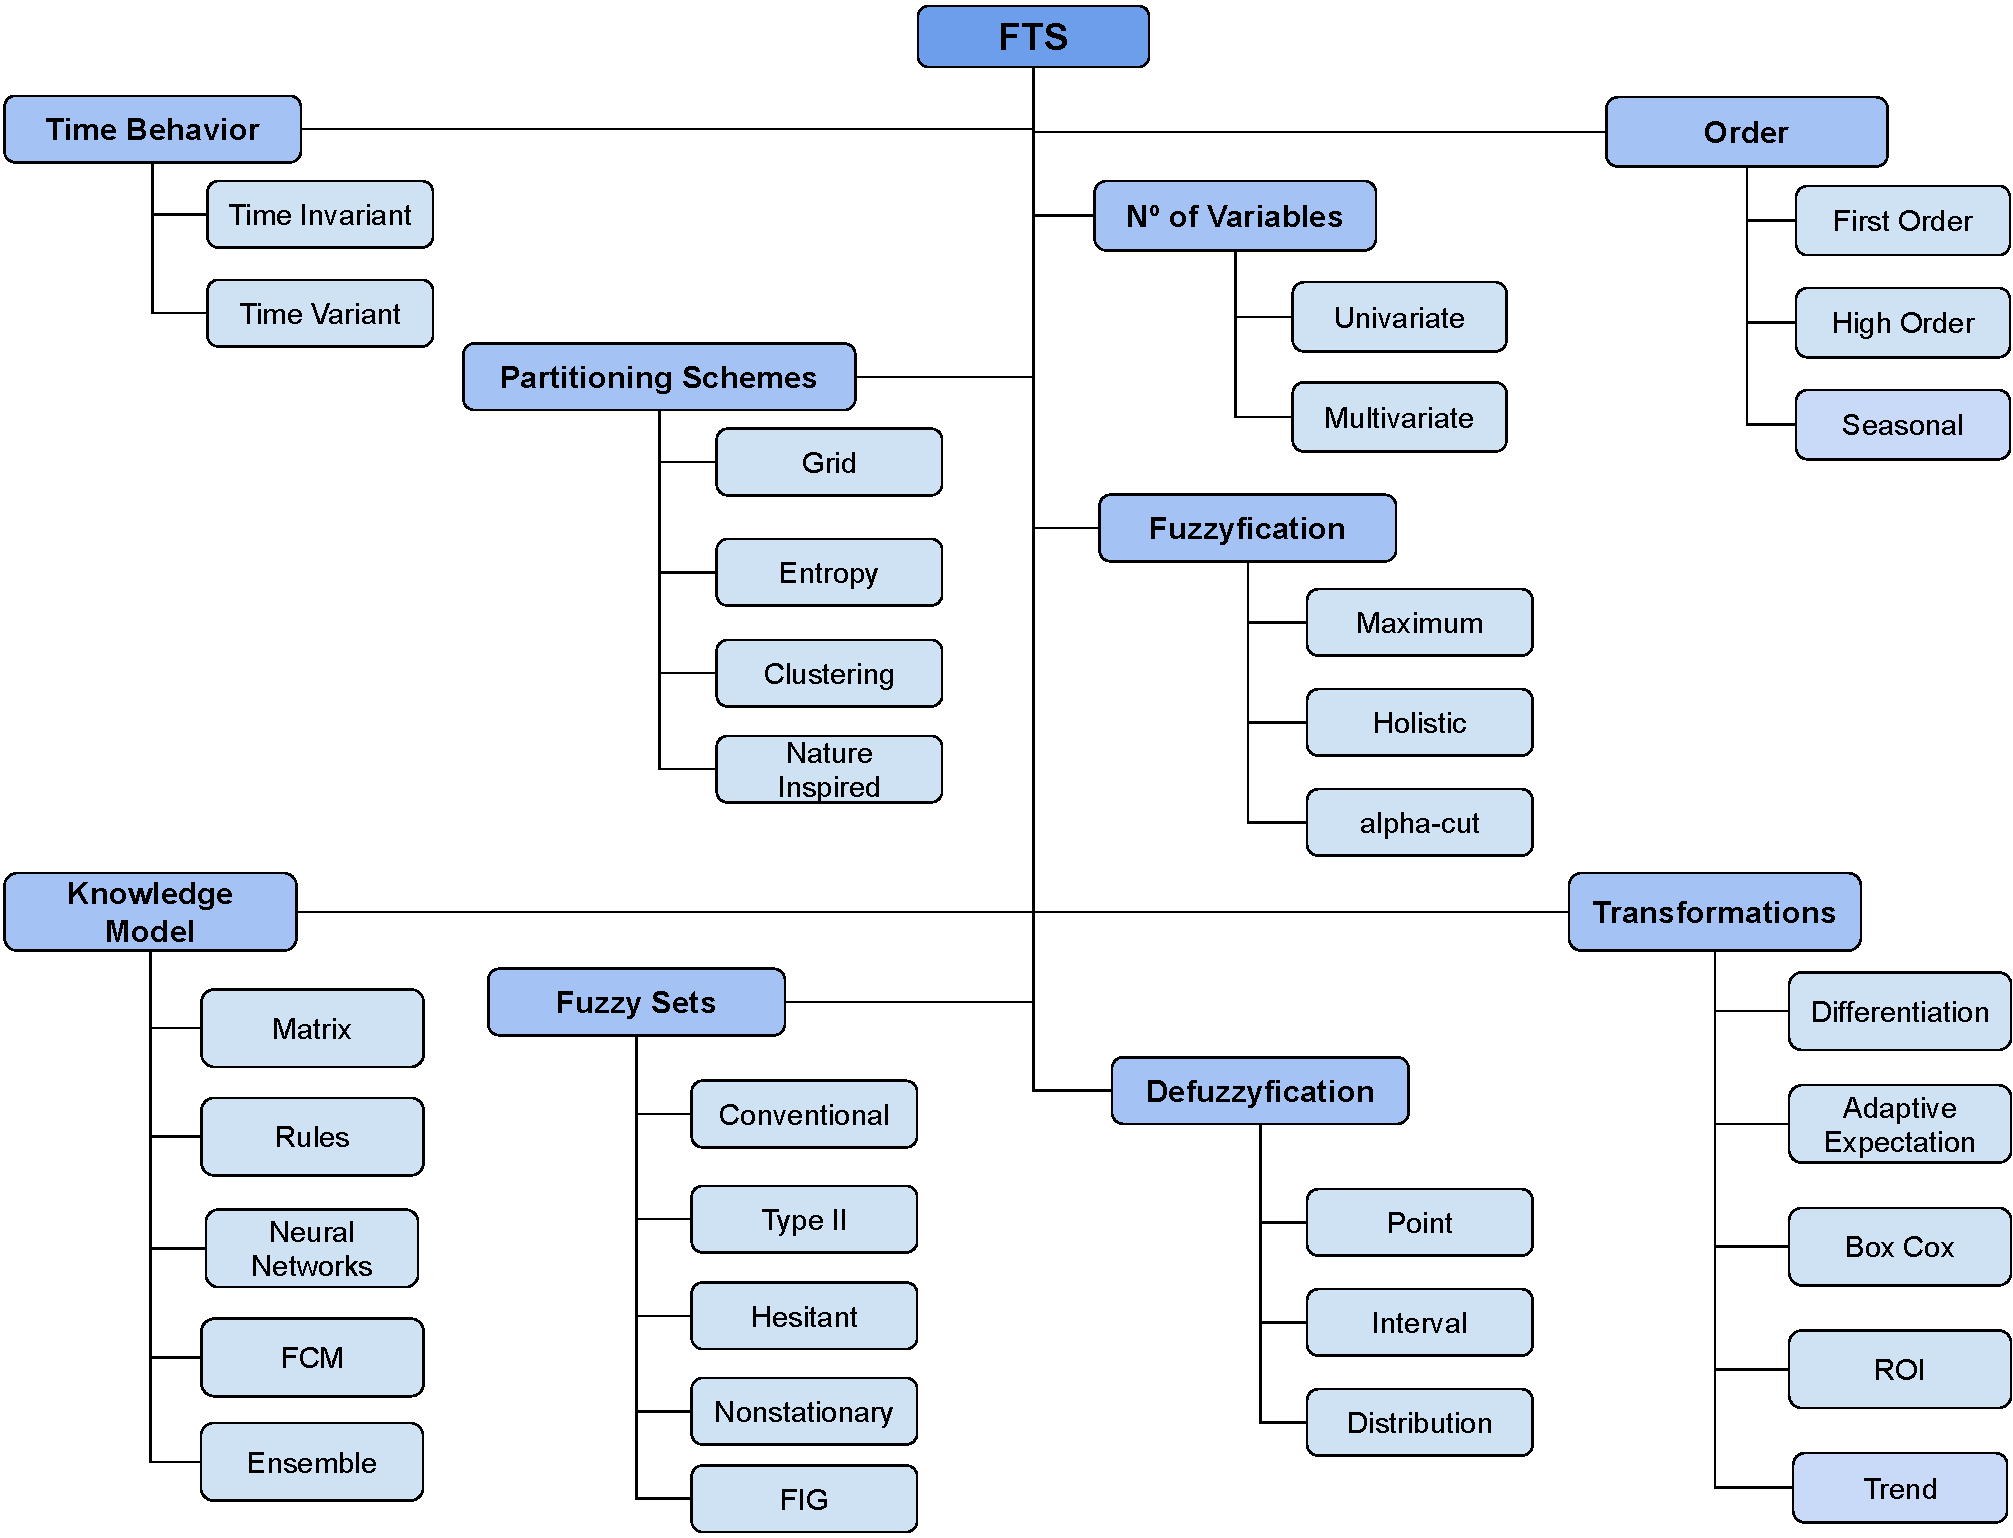
\includegraphics[width=\textwidth, height=15cm]{figures/fts_taxonomy.pdf}
    \caption{A brief taxonomy of FTS methods}
    \label{fig:fts_taxonomy}
\end{figure}

The most important categories of FTS methods are related with their the time behavior. The time invariant models are the ones used when the Universe of Discourse and data behavior  does not change with time, as in stationary time series. Non stationary time series, in its turn, require time variant models as proposed in \cite{Song1994} and \cite{Wong2010}. This research is focused on time invariant models and hereinafter all models discussed belongs to it. However, Time Variant models are not discarded for future investigations.

The main contributions of this chapter are the proposals of two consensus methods, which aggregate the major developments of the FTS literature for high order rule based and weighted rule based methods: the High Order Fuzzy Time Series (HOFTS) and the Weighted High Order Fuzzy Time Series (WHOFTS). These methods are intended for point forecasting, for one to many steps ahead.

This chapter also focus only on monovariate and non Big Data time series. The multivariate and Big Data methods will be discussed in the following chapters. In the next section the main processes of the FTS are introduced and discussed.

%%%%%%%%%%%%%%%%%%%%%%%%%%%%%%%%%%%%%%%%%%%%%%%%%%%%%%%%%%%%%%%%%%%%%%%%%%%%
%%%%%%%%%%%%%%%%%%%%%%%%%%%%%%%%%%%%%%%%%%%%%%%%%%%%%%%%%%%%%%%%%%%%%%%%%%%%

\section{Fuzzy Time Series common processes}
\label{sec:common_fts} \index{Common Fuzzy Time Series processes}\index{FTS process}

\index{Universe of Discourse}\index{UoD}\index{Fuzzy Time Series}\index{FTS}

The definition of Fuzzy Time Series, from \cite{song1993fuzzy}, starts with a univariate time series $Y \in \mathbb{R}^1$, for $t = 0,1,...,T$, where the Universe of Discourse $U$ is delimited by the known bounds of $Y$, such that $U = [\min(Y),\max(Y)]$. Upon $U$, $k$ fuzzy sets $\ufset$, for $j = 1..k$, are defined and each one with its own membership function $\mu_{\ufset}$. $F$ is called a Fuzzy Time Series over $Y$ if $f(t) = \mu_{\ufset}(y(t))$ is the collection of fuzzyfied values of $Y$ for $j = 1..k$ and $t = 0,1,...,T$. The group of fuzzy sets $\ufset$, for $j = 1..k$, can also be understood as a Linguistic Variable $\ulvar$, and each fuzzy set $\ufset \in \ulvar$ is a linguistic value of the linguistic variable. 
\index{Linguistic Variable}

\begin{figure}[htb]
    \centering
    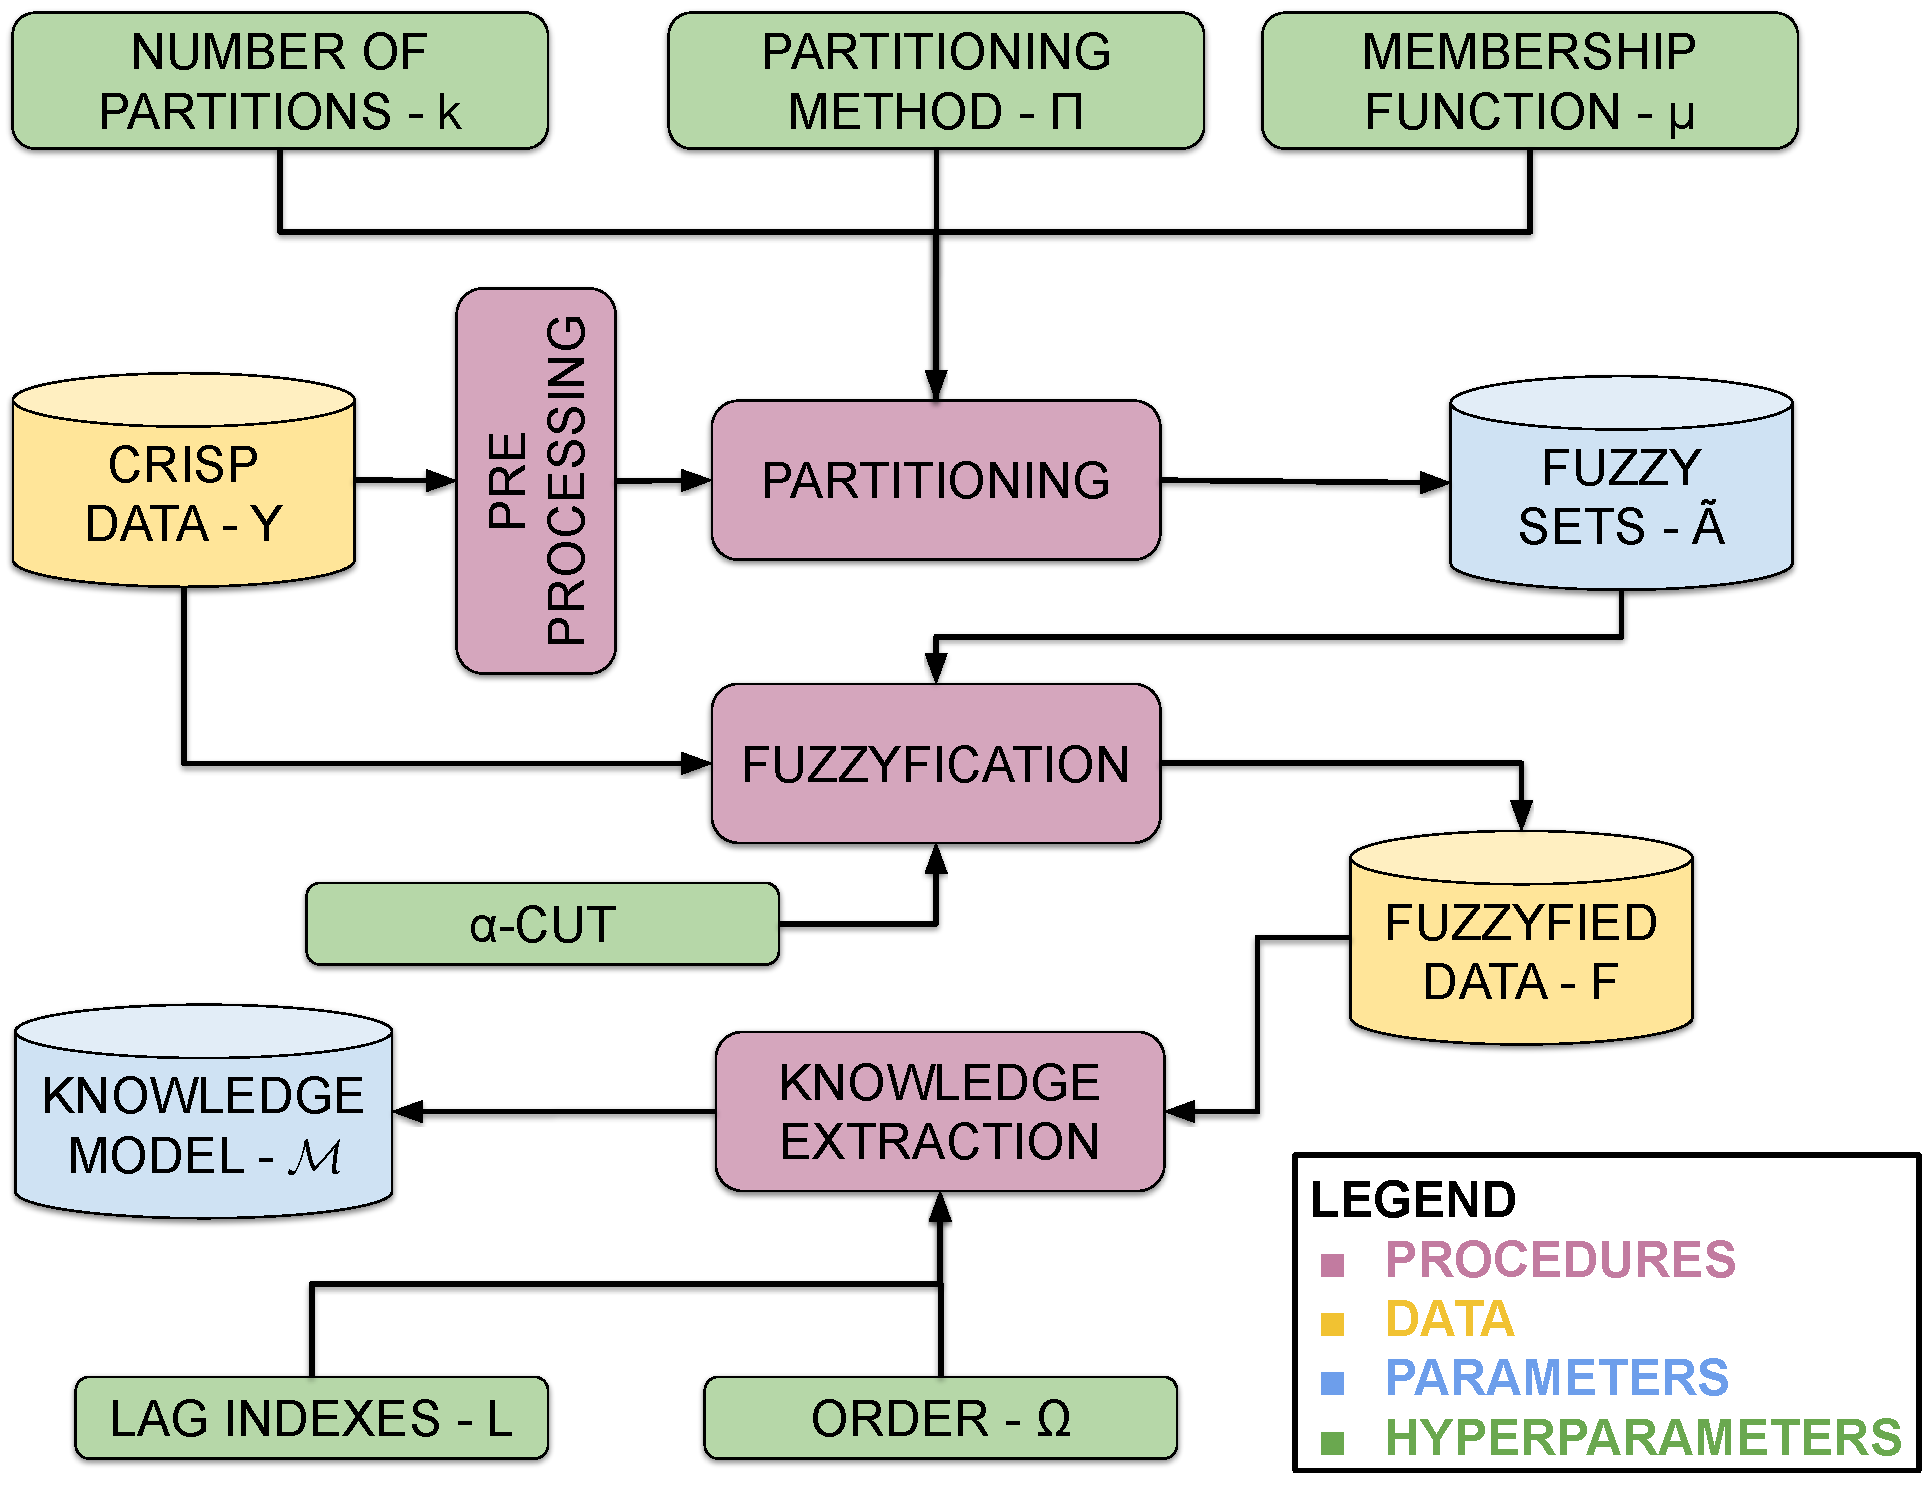
\includegraphics[width=\textwidth]{figures/fts_training.pdf}
    \caption{Generic time invariant Fuzzy Time Series training procedure and its components}
    \label{fig:fts_training}
\end{figure}

\cite{Song1993partI} proposed the first FTS methodology and the following authors basically extended or modified some steps of the method. A generic method can be extracted from the wide range of variations of FTS methods by splitting the FTS approach in two main procedures, the training and forecasting methods. The training method, illustrated in Figure \ref{fig:fts_training}, has the basic objective to create the linguistic variable $\ulvar$ and a knowledge representation of the time series dynamics. These two objects compose the FTS model $\model$. The main components of this process are listed below:

\begin{enumerate}
    \item[Step 1] - \textbf{Pre-processing}: First, one or more pre-processing data transformations can be applied to input data $Y$, responsible to reduce noise, detrending, or de-seasonalize, or change the $U$, etc. Several methods contain these operators and their impact will be discussed in detail in Section \ref{sec:fts_transformations}.
    
    \item[Step 2] - \textbf{Partitioning}: The most important process of the training is executed, the partitioning. This process is responsible to split the universe of discourse $U$ into $k$ fuzzy sets $\ufset$, creating the linguistic variable $\ulvar$ used to describe $Y$. There are many ways that the partitioning can be performed, and the most important are discussed in Section \ref{sec:fts_partitioning}.
    
    \item[Step 3] - \textbf{Fuzzyfication}: With the linguistic variable $\ulvar$ the crisp data $Y$ can be transformed in a linguistic representation, the fuzzy time series $F$ where each $f(t) \in F$ is a fuzzyfied version of $y(t) \in Y$. Details of the fuzzyfication are discussed in Section \ref{sec:fts_fuzzyfication}.
    
    \item[Step 4] - \textbf{Knowledge Extraction and Representation}: The second most important process is the knowledge extraction. This process is responsible to induce the knowledge model $\model$ by performing a pattern recognition over $F$ and learning the temporal patterns between  $\Omega$ lags, whose indexes are identified by $L$, and their consequent ones. The most important learning algorithms and knowledge models are discussed in Section \ref{sec:fts_knowledge}.
\end{enumerate}

Once the linguistic variable $\ulvar$ is defined and the FTS model $\model$ was learned, new samples $y(t) \in U$ can be presented to produce a forecast $\hat{y}(t+1)$. The generic forecasting procedure is illustrated in Figure \ref{fig:fts_forecasting}, and its main components are listed below:

\begin{enumerate}
    \item [Step 1] - \textbf{Pre-processing}: First, one or more pre-processing and post-processing data transformations can be applied to input sample $y(t)$ (the data transformations are discussed in Section \ref{sec:fts_transformations}).
    
    \item[Step 2] - \textbf{Fuzzyfication}: The fuzzyfication procedure follows the same schema of the training procedure and it is discussed in Section \ref{sec:fts_fuzzyfication}. 
    
    \item[Step 3] - \textbf{Inference}: The inference engine deeply depends on the knowledge model $\model$. Indeed, the learning algorithm, the knowledge model and the inference engine are intrinsically correlated, and they are discussed in Section \ref{sec:fts_knowledge}. The aim of the inference process is to produce $f(t+1)$, candidate fuzzy sets (and other additional information, as weights) to represent the future crisp value $y(t+1)$.
    
    \item[Step 4] - \textbf{Deffuzyfication}: The deffuzyfication process aims to transform the $f(t+1)$ to a crisp numeric estimate $\estimate$ for the real (but unknown) value $y(t+1)$. The deffuzyfication usually also depends on the inference engine but there are common methods discussed in Section \ref{sec:fts_defuzzyfication}. The present work extended the possibilities of deffuzyfication to beyond of point forecasting, proposing methods for prediction intervals $\mathbb{I}$ and probabilistic distributions $P$.
    
    \item [Step 5] - \textbf{Post-processing}: Finally, one or more post-processing data transformations can be applied to output forecast $\estimate$  (the data transformations are discussed in Section \ref{sec:fts_transformations}).
\end{enumerate}

\begin{figure}
    \centering
    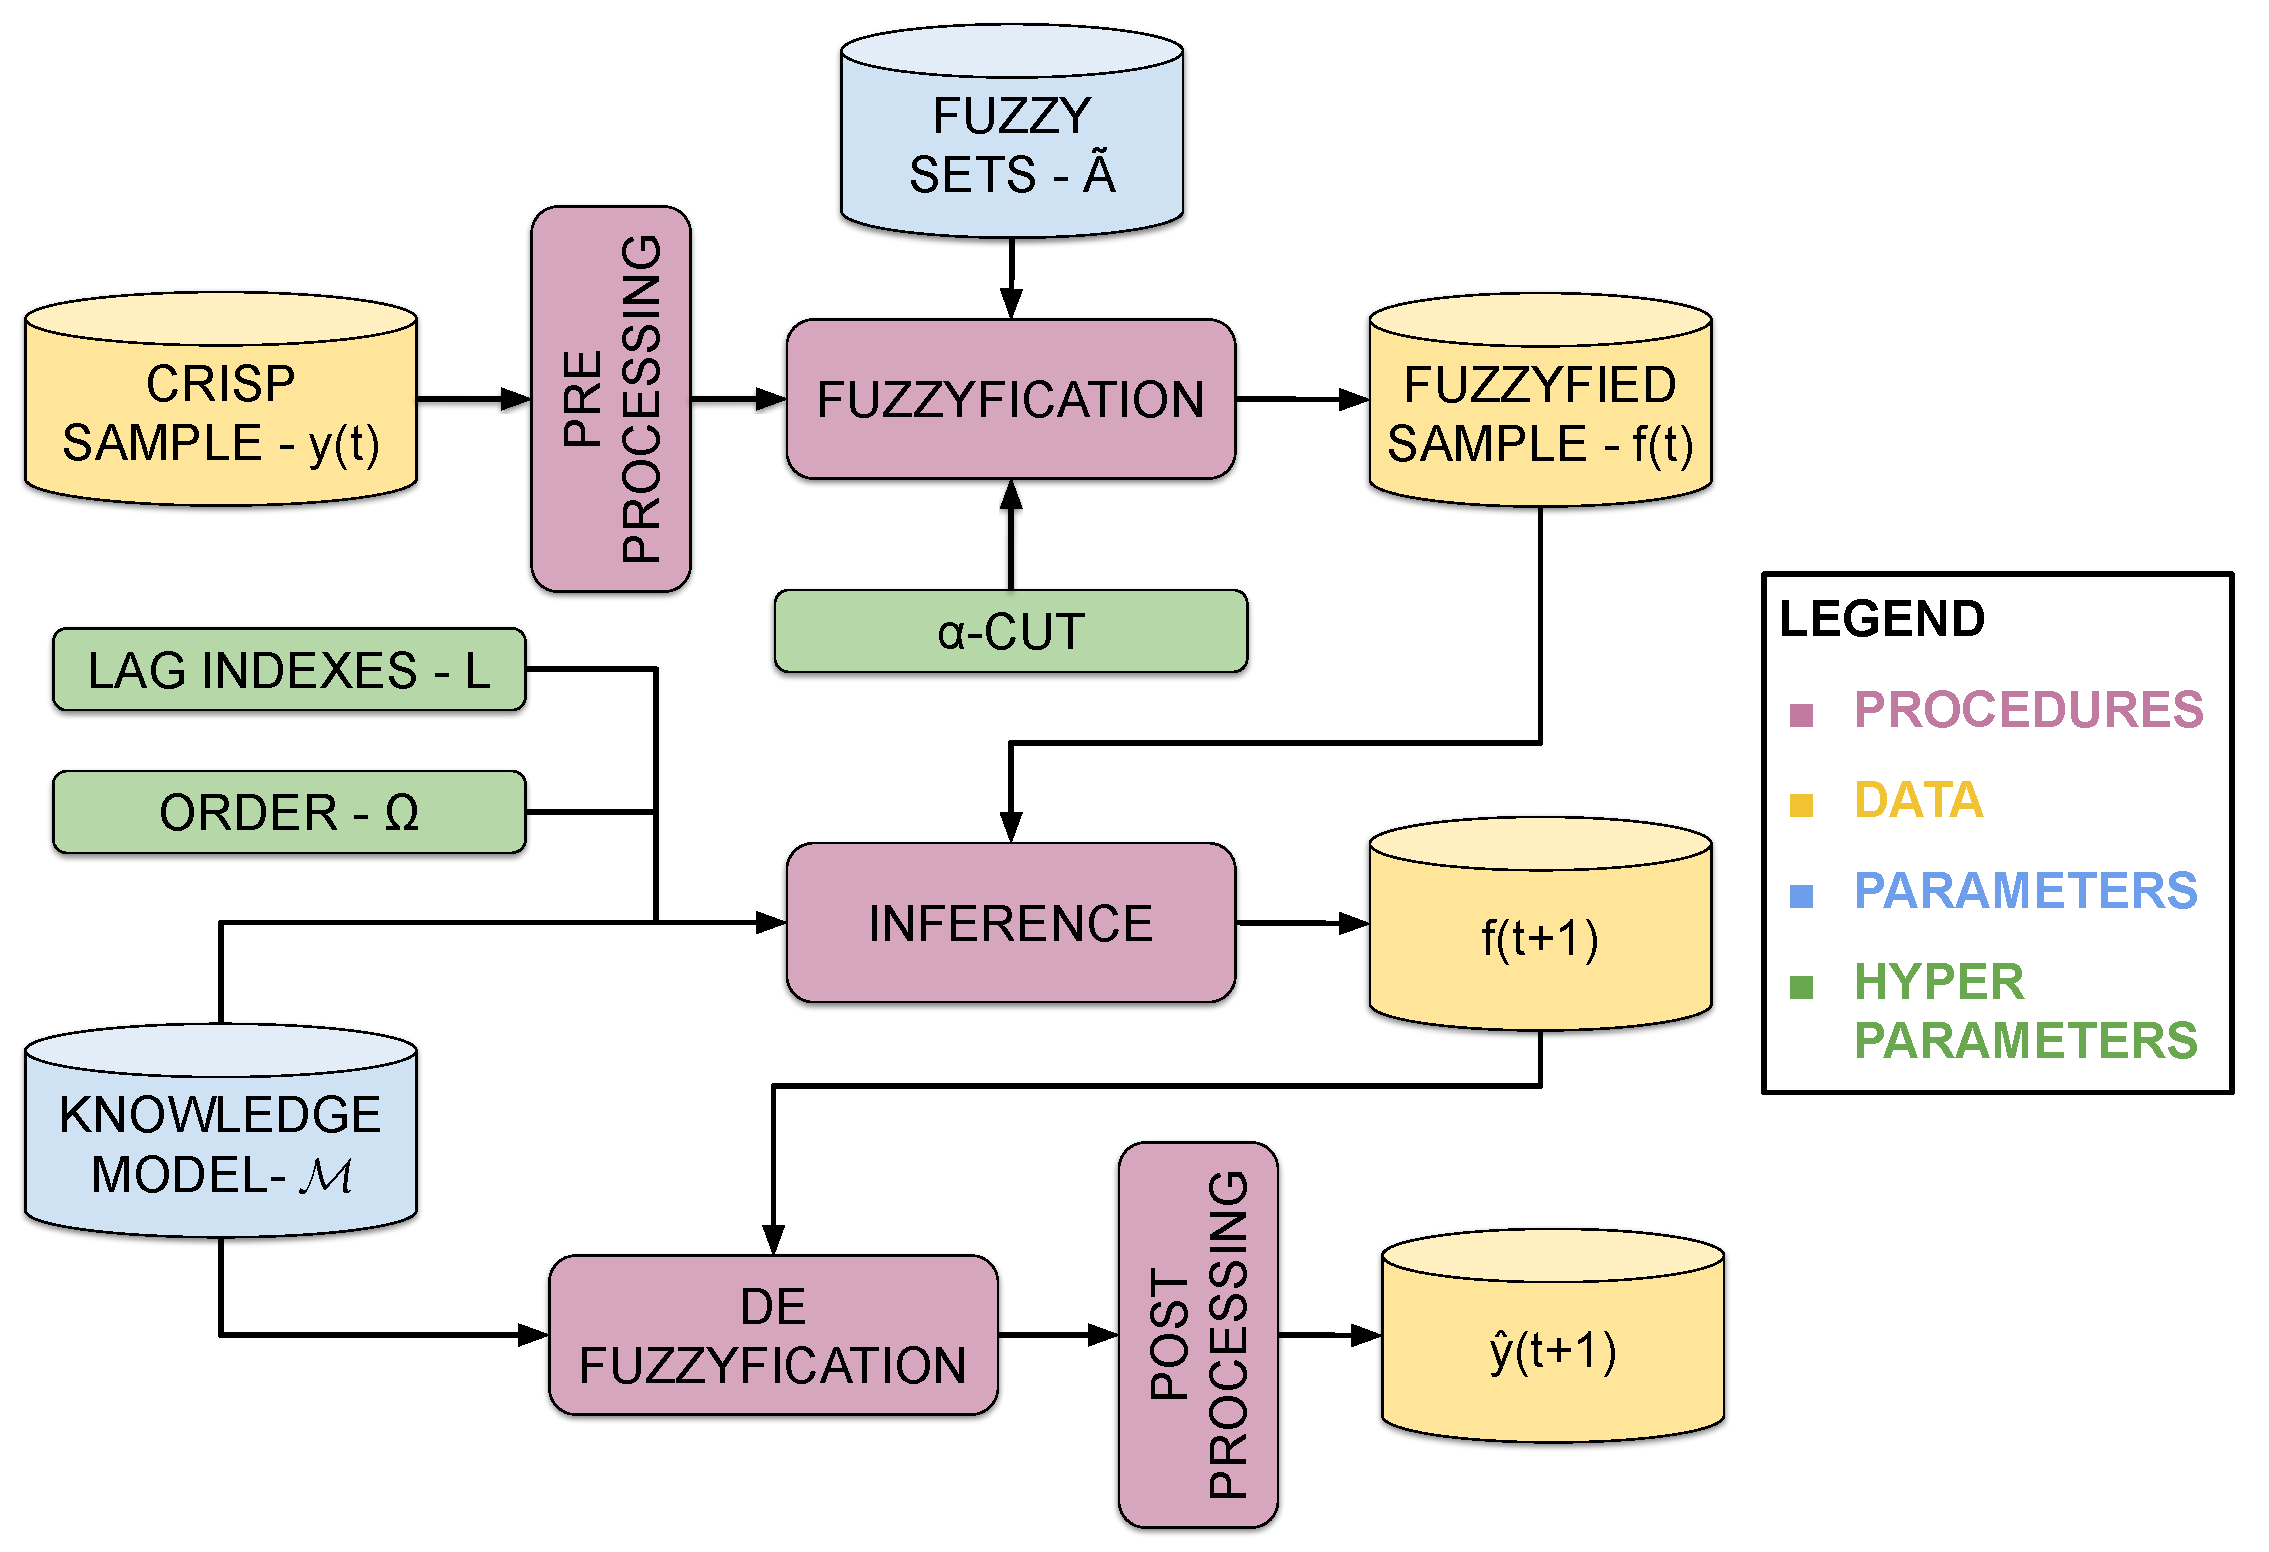
\includegraphics[width=\textwidth,height=12cm]{figures/fts_forecasting.pdf}
    \caption{Generic time invariant Fuzzy Time Series forecasting procedure and its components}
    \label{fig:fts_forecasting}
\end{figure}


The main hyperparameters which affect these processes are listed in Table \ref{tab:fts_hyperparameters}. The selection of the values for these hyperparameters affects the training process and the parameters of the model, including its accuracy and parsimony (the length of the model).  In the following sections each one of these processes are discussed in detail recurring to the most relevant works in the FTS literature, while its strengths and drawbacks are highlighted.

\begin{table}[]
    \centering
    \begin{tabular}{|c|m{7cm}|m{5cm}|} \hline
        \textbf{Alias} & \textbf{Parameter}& \textbf{Process} \\ \hline
         $k \in \mathbb{N}^+$ & Number of partitions (fuzzy sets) & Universe of Discourse Partitioning \\ \hline
         $\mu: U \rightarrow [0,1] $ & Membership function, measures the membership of a value $y \in U$ to a fuzzy set & Universe of Discourse Partitioning, Fuzzyfication  \\\hline
         $\Pi$ & Partitioning method & Universe of Discourse Partitioning \\\hline
         $\alpha \in [0,1]$ & the $\alpha$-cut, the minimal membership grade to take account on fuzzyfication process & Fuzzyfication \\ \hline
         $\Omega \in \mathbb{N}^+$ & Order, the number of lags & Knowledge model  \\\hline
         $L \in \Omega \times \mathbb{N}^-$ & Time lag indexes & Knowledge model \\\hline
    \end{tabular}
    \caption{Common hyperparameters for FTS methods}
    \label{tab:fts_hyperparameters}
\end{table}

\index{Hyperparameter}

%%%%%%%%%%%%%%%%%%%%%%%%%%%%%%%%%%%%%%%%%%%%%%%%%%%%%%%%%%%%%
%
%%%%%%%%%%%%%%%%%%%%%%%%%%%%%%%%%%%%%%%%%%%%%%%%%%%%%%%%%%%%%
\section{Universe of Discourse Partitioning}
\label{sec:fts_partitioning}
\index{UoD Partitioning}\index{Partitioning Schemes}

This process aims to split the Universe of Discourse $U$ and to create the linguistic variable $\ulvar$, composed by the fuzzy sets $\ufset$, $j = 1 .. k$. This is the most important process of the FTS approach and the following sections detail its main sub-processes and parameters.

%%%%%%%%%%%%%%%%%%%%%%%%%%%%%%%%%%%%%%%%%%%%%%%%%%%%%%%%%%%%%
%
%%%%%%%%%%%%%%%%%%%%%%%%%%%%%%%%%%%%%%%%%%%%%%%%%%%%%%%%%%%%%
\subsection{Universe of Discourse $U$}
\label{sec:fts_uod} \index{Universe of Discourse}\index{$U$}\index{UoD}

The natural definition of the Universe of Discourse is $U = [\min(Y),\max(Y)]$, but it is common that the upper and lower bounds be exceeded by a confidence margin. Then, it can be established as $U = [\underline{l}, \overline{u}]$, with the lower bound as $\underline{l} = \min(Y) + l_d$, where $l_d = \min(Y)\cdot 0.2$ (exceeding the original lower bound by 20\%) and the upper bound as $\overline{u} = \max(Y) + u_d$, where $u_d = \max(Y)\cdot 0.2$ (exceeding the original upper bound by 20\%). 

Even considering just time invariant methods in this work and a stationary time series $Y$, it is natural that the testing $U$ will be a little different from the training $U$, sometimes by a small fraction of the original values. Even on stationary processes the presence of outliers cannot be discarded. The objective of these exceeding margins $l_d$ and $u_d$ is to help in the fuzzyfication process of the forecasting procedure, in order to accommodate fluctuations in the bounds of the known $U$.

%%%%%%%%%%%%%%%%%%%%%%%%%%%%%%%%%%%%%%%%%%%%%%%%%%%%%%%%%%%%%
%
%%%%%%%%%%%%%%%%%%%%%%%%%%%%%%%%%%%%%%%%%%%%%%%%%%%%%%%%%%%%%
\subsection{Membership function $\mu$}\index{Membership function}\index{$\mu$}\index{Fuzzy sets}
\label{sec:fts_membership}

Once $U$ has been defined, three hyperparameters will determine the creation of $\ulvar$: the number of partitions $k$, the membership function $\mu$ and the partitioning scheme. The membership function $\mu: U \rightarrow [0,1]$ defines how much a crisp value belongs to a fuzzy set, in terms of the membership grade $[0,1]$. Some options of fuzzy membership functions are shown in Table \ref{tab:fts_membership}, and simple partitioning using these functions are shown in Figure \ref{fig:membership}. The real impact of the membership function on accuracy is low, it will be demonstrated empirically later on this work, but the chosen of the correct $\mu$ can help in the readability and explainability of the model.

Many other kinds of fuzzy sets were presented in the literature and new FTS methods were developed using them, as instance Type 2 fuzzy sets \citep{huarng2005type, Bajestani2011}, Hesitant fuzzy sets \citep{Bisht2016}, non-stationary fuzzy sets \citep{Alves2018}, etc. These fuzzy sets and the methods developed with them, however, are considered out of the scope of this research.

\index{Membership function}\index{$\mu$}
\begin{table}[]
    \centering
\begin{tabular}{|c|m{4cm}|c|} \hline
\textbf{Name}  & \textbf{Parameters}  & \textbf{Definition} \\ \hline
Singleton  & $c$, the central value & 
$\mu(x,c) = \left\{ \begin{array}{ccc}
        1 & if & x = c  \\
        0 & if & x \neq c
    \end{array}\right.$ \\ \hline
Triangular  & $a$: lower bound, $b$: midpoint, $c$: upper bound  & 
$\mu(x,a,b,c) = \left\{ \begin{array}{ccc}
        0 & if & x \leq a  \\
        \frac{x-a}{b-a} & if & a \leq x \leq b  \\
        \frac{c-x}{c-b} & if & b \leq x \leq c  \\
        0 & if & c \geq x
    \end{array}\right.$ \\ \hline
Trapezoidal  & $a$: lower bound, $b$: top-left, $c$: top-right, $d$ upper bound & 
$\mu(x,a,b,c,d) = \left\{ \begin{array}{ccc}
        0 & if & x \leq a  \\
        \frac{x-a}{b-a} & if & a \leq x \leq b  \\
        1 & if & b \leq x \leq c  \\
        \frac{d-x}{d-c} & if & c \leq x \leq d  \\
        0 & if & d \geq x
    \end{array}\right.$ \\ \hline
Gaussian  & $m$: midpoint, $d$: spread & 
$\mu(x,m,d) = \exp \left(-\frac{(x-d)^2}{2m^2}\right)$ \\ \hline
\end{tabular}
\caption{Most common fuzzy membership functions}
    \label{tab:fts_membership}
\end{table}

\begin{figure}
    \centering
    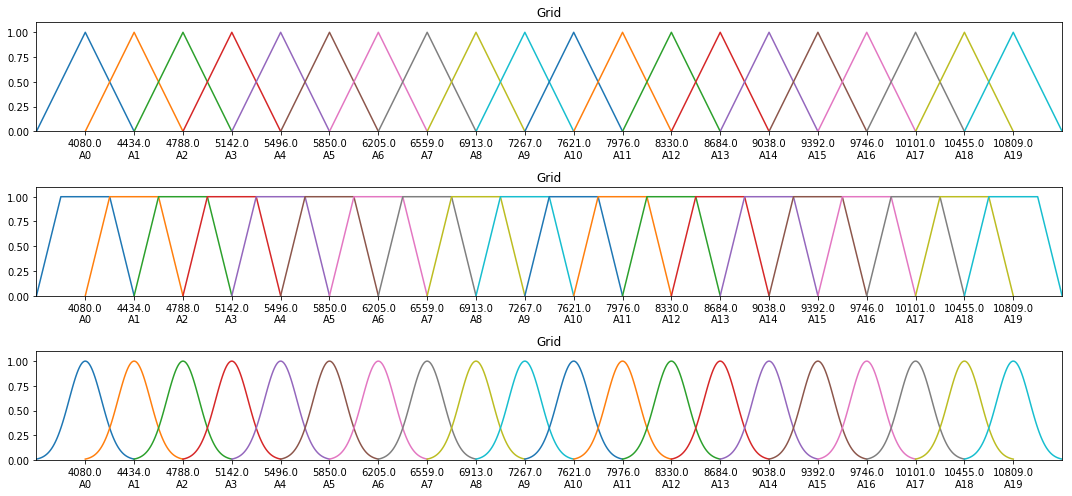
\includegraphics[width=\textwidth]{figures/membership.png}
    \caption{UoD Partitioning using different membership functions}
    \label{fig:membership}
\end{figure}

%%%%%%%%%%%%%%%%%%%%%%%%%%%%%%%%%%%%%%%%%%%%%%%%%%%%%%%%%%%%%
%
%%%%%%%%%%%%%%%%%%%%%%%%%%%%%%%%%%%%%%%%%%%%%%%%%%%%%%%%%%%%%
\subsection{The number of partitions $k$}\index{Number of partitions}\index{$k$}
\label{sec:fts_partitions}

\index{overfit}\index{underfit}\index{Hyperparameter Optimization}\index{model accuracy}\index{model performance}
The selection of the hyperparameter $k$ impact directly on the model accuracy and parsimony, as discussed in \cite{Duru2012}. The number of partitions impact on the model parsimony directly and, for instance, given a rule model the maximum number of rules is the cartesian product between the fuzzy sets $\ufset \in \ulvar$ for each order $\Omega$. 

There is a non-linear relationship between $k$ and the model accuracy, a trade off between specific accuracy (bias) and overall generalization (variance). A small value of $k$ will generate too few fuzzy sets to represent $Y$ correctly, making the model $\model$ underfit by producing a gross generalization with simplistic patterns. A high value of $k$ will generate too much fuzzy sets, exceeding the needed to represent $Y$ and makeing the model $\model$ overfit by reproducing excessive specificities and small noisy fluctuations. The optimal number of $k$ must be optimized for each problem, balancing the accuracy and the model parsimony, since this last value affects the computational performance as the number of parameters grows.

The impact of the $U$ partitioning can also be seen by other perspectives: the model human readability and model explainability. In his seminal work, \cite{Miller1956} stated that the human being, on average, can learn $7 \pm 2$ concepts. In other words, the linguistic variable $\ulvar$ to be reasonable for human understanding must have around this number of fuzzy sets. But this, depending on the range of $U$ and the behavior of $Y$, may be a very small number of partitions. Otherwise, the explainability does not depend on how much humans can learn from $\model$ but how easily the forecastings produced can be explained, as a white box model. In this last case the type of the knowledge representation of $\model$ has greater impact than the number of fuzzy sets in $\ulvar$. 

A study of the linguistic characterization of time series can be found in \cite{Novak2016}. using Fuzzy Transform (\cite{Perfilieva2006}) to generate linguistic summaries of time series. A study on mining information from fuzzyfied linguistic time series can be found in \cite{Novak2016a}, where are presented the impacts of fuzzyfication on the knowledge extraction.

%%%%%%%%%%%%%%%%%%%%%%%%%%%%%%%%%%%%%%%%%%%%%%%%%%%%%%%%%%%%%
%
%%%%%%%%%%%%%%%%%%%%%%%%%%%%%%%%%%%%%%%%%%%%%%%%%%%%%%%%%%%%%
\subsection{The partitioning method - $\Pi$}\index{UoD Partitioning}\index{Partitioning Method}\index{$\Pi$}\index{Fuzzy sets}
\label{sec:fts_partitioningmethod}

The partitioning method will determine, for each fuzzy set,  their length, midpoints and bounds and also have impact on accuracy. The simplest partitioning scheme -- the division of the data range in $k$ equal length intervals -- is called Grid Partitioning and was proposed in \cite{song1993fuzzy}. \index{Grid Partitioning} In the Grid Partitioning, $U$ is divided in $k+2$ even intervals $u_1, u_2, ..., u_k$ whose midpoints are $c_1, c_2, ..., c_k$. Then with these $k$ intervals $k$ overlapped fuzzy sets $A_1,A_2,...,A_k$ are defined using triangular membership functions whose parameters are $c_{j-1},c_j,c_{j+1}$ for each $j = 2..k-1$. 

Some works used simple heuristics to define $k$ or even the lengths of the fuzzy sets. \cite{huarng2001effective}\index{Huarng Partitioning}\index{Heuristic Partitioning} use a grid partitioning approach, but it proposes an empirical method to find the ideal number of partition lengths according to the magnitude of $U$, in a work that was the first to deeply discuss the impact of the partitioning on FTS forecast accuracy. Several other works used this or define other simple heuristic for $U$ partitioning, see for instance \cite{Chang1997, huarng2005type, Rubio2016, Cheng2018}.

$U$ partitionings where the fuzzy sets have unequal lengths are also present in the literature. \cite{Cheng2006a} employ a fixed value of $k$ but the entropy of data that defines the best midpoints for the fuzzy sets, which also use trapezoidal membership functions. This method is known by Entropy Partitioning and is also employed in \cite{Cheng2008} and \cite{Chen2014}.\index{Entropy Partitioning} The statistical approaches yet count with \cite{Ismail2015}, which determine the length of the fuzzy sets proposing a method based on data quantiles, and \cite{Yang2017} which use a Chi-Square distribution do identify the fuzzy sets number and lengths.

Clustering techniques are used in several works, as Fuzzy C-Means in \cite{Li2008b, Askari2015, Bas2015, Sun2015, Yolcu2017}, Fuzzy K-Medoids in \cite{Dincer2018}, Self Organizing Maps in \cite{Bahrepour2011}, and other methods as in \cite{Saberi2017} and \cite{Bose2017}.\index{FCM Partitioning}\index{Cluster Partitioning}

The use of metaheuristics, especially of nature-inspired optimization approaches, is also spread in the literature. Particle Swarm Optimization is used by \cite{Davari2009, Kuo2009, Hsu2010, Huang2011, Zhang2018a}, Genetic Algorithms in \cite{Chen2006a, Enayatifar2013, Zhang2018}, and other less known methods such as Harmony Search in \cite{Talarposhti2016a, Jiang2017} and Imperialist Competitive in \cite{Sadaei2017}. \index{Evolutionary Partitioning}\index{Metaheuristic Partitioning}\index{PSO Partitioning}

\begin{figure}
    \centering
    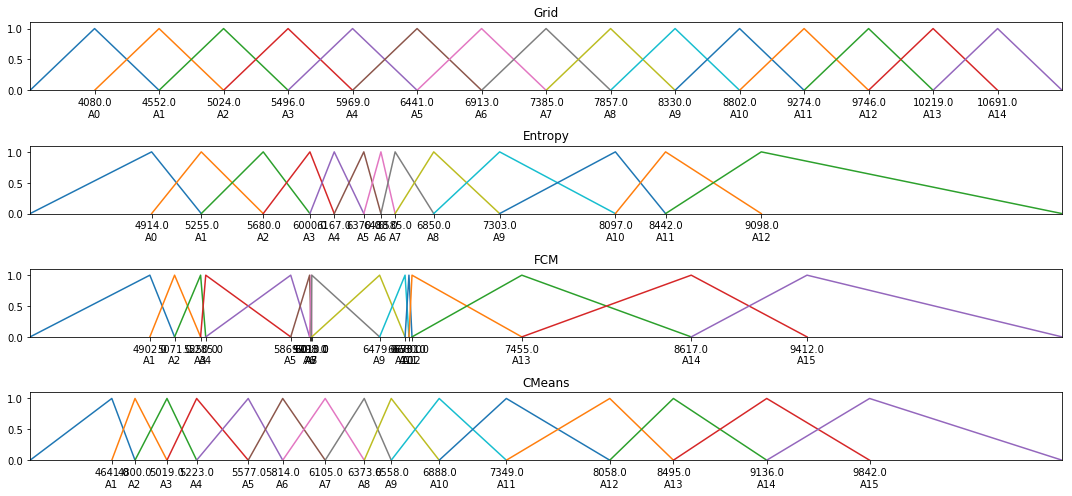
\includegraphics[width=\textwidth]{figures/partitioners.png}
    \caption{Partitioning using different approaches within the same sample}
    \label{fig:partitioners}
\end{figure}

A sample of different partitioning schemes on the same data can be seen in Figure \ref{fig:partitioners}. The partitioning method has influence on the model accuracy, parsimony and readability but its computational cost must be also considered. The Grid Partitioning gives a uniform distribution of the fuzzy sets over $U$ but, if in one hand it is computationally cheaper, however it may not represent the importance of some data regions accordingly. It is probable that some specific regions of $U$ have more variance than others, depending on $Y$ behavior, and some regions may be better represented having more fuzzy sets than others. It also can not be denied that some approaches are computationally expensive, as the clustering and metaheuristics ones, and in Big Data scenarios this may be prohibitive. Despite the fact that the Grid Partitioning should be always the first approach to start with, due to its simplicity and small cost, the fine tuning of FTS models can not exclude more sophisticated methods.

Once the linguistic variable $\ulvar$ is created, the fuzzyfication process can be started. This process and its parameters are discussed in the next section.


%%%%%%%%%%%%%%%%%%%%%%%%%%%%%%%%%%%%%%%%%%%%%%%%%%%%%%%%%%%%%
%
%%%%%%%%%%%%%%%%%%%%%%%%%%%%%%%%%%%%%%%%%%%%%%%%%%%%%%%%%%%%%
\section{The Fuzzyfication Process}
\label{sec:fts_fuzzyfication}
\index{Fuzzyfication Method}\index{Fuzzy sets}

This process aims to transform the crisp numerical time series $Y$ into a linguistic time series $F$, also known as fuzzy time series. There are few, but important, variations of the fuzzyfication method.

The initial FTS methods, for instance \cite{song1993fuzzy}, \cite{chen1996forecasting} and \cite{yu2005weighted}, only considered one fuzzy set in fuzzyfication process, for instance $y(t) \in Y$, the one with the greatest membership grade. More specifically:
\index{Maximum membership fuzzyfication}

\begin{equation}
f(t) = \ufset\; |\; \mu_{\ufset}(y(t)) = \max\{ \mu_{A_1}(y(t)), \ldots, \mu_{A_k}(y(t)) \}    
\label{eqn:fuzzyfication_maximum}
\end{equation}

\index{overfit}\index{underfit}
This method helps to control overfit, reducing the number of spurious patterns generated by low membership grades fuzzy sets. However, it can also contribute to underfit the learning by eliminating fuzzy sets which are very close to the maximum grade. It is possible to deduce that some relevant information can be lost when several minor membership grades are discarded.

A contrasting method is the holistic fuzzyfication, where all the membership grades, despite their magnitude, are considered. The fuzzyfied value $f(t)$ is the the vector of the $y(t)$ membership grades with respect to each $\ufset \in \ulvar$:

\begin{equation}
f(t) = [\mu_{A_1}(y(t)), \ldots, \mu_{A_k}(y(t)) ]    
\label{eqn:fuzzyfication_holistic}
\end{equation}

\index{Alpha cut}\index{$\alpha$-cut}\index{Holistic fuzzyfication}
The holistic fuzzyfication can help to the learning overfit, because even very small membership grades, which can be considered insignificant for that fuzzy set, are considered. An intermediate approach can be achieved by using the $\alpha$-cut hyper-parameter. The $\alpha$-cut represents the minimal value of the membership grade that will be accepted in fuzzyfication, while membership values below the $\alpha$-cut will not be considered. 

\begin{equation}
f(t) = \ufset\; |\; \mu_{\ufset}(y(t)) \geq \alpha \;\; \forall \ufset \in \ulvar    
\label{eqn:fuzzyfication_alpha}
\end{equation}

The $\alpha$-cut makes the sensibility of the fuzzyfication process adjustable and the user can control it, unlike the maximum membership and the holistic methods. The fuzzyfication method is significant in the search of the training best fit, controlling the accuracy and models parsimony. Particularly, the method of \cite{CarvalhoJr2017} makes an explicit use of the $\alpha$-cut parameter and conduct a comprehensive study of its impact on the method accuracy.

Once the crisp data $Y$ is converted to the fuzzy time series $F$ the process of knowledge extraction and representation is ready to start. This process and its variations are discussed in the next section.

%%%%%%%%%%%%%%%%%%%%%%%%%%%%%%%%%%%%%%%%%%%%%%%%%%%%%%%%%%%%%
%
%%%%%%%%%%%%%%%%%%%%%%%%%%%%%%%%%%%%%%%%%%%%%%%%%%%%%%%%%%%%%
\section{Knowledge Extraction, Representation and Inference}
\label{sec:fts_knowledge}
\index{Knowledge extraction}\index{Knowledge representation}
\index{Inference}\index{Induction}

This section aims to investigate the several approaches in the literature that were used to learn and represent temporal patterns found on the fuzzyfied data $F$. Looking back to Figures \ref{fig:fts_training} and \ref{fig:fts_forecasting}, the fuzzy sets and the fuzzyfication process may be interpreted as a feature extraction layer that precedes a pattern recognition and inference layer, that is finally succeeded by a reconstruction layer -- the deffuzyfication process. Besides small variations, the fuzzyfication and deffuzyfication do not differ among the methods. But the way these methods learn and store the patterns suffer a strong variation among them.

By far, most of FTS methods make use of simple heuristics to learn the temporal patterns from the fuzzyfied data and store the learned patterns using rules or matrices. But it can not be denied that there are many other backends for the knowledge extraction and representation in FTS models: metaheuristics, neural networks, fuzzy cognitive models, hybrid approaches with traditional statistical models, etc. In the following sections the most relevant methods with their variations will be discussed. 

%%%%%%%%%%%%%%%%%%%%%%%%%%%%%%%%%%%%%%%%%%%%%%%%%%%%%%%%%%%%%
%
%%%%%%%%%%%%%%%%%%%%%%%%%%%%%%%%%%%%%%%%%%%%%%%%%%%%%%%%%%%%%
\subsection{The Order $\Omega$, Lags $L$ and Seasonality}
\label{sec:fts_order}\index{High Order Models}\index{Lags}\index{Seasonal Models}\index{$\Omega$}\index{$L$}

First it is needed to consider the hyperparameters order $\Omega$ and the lag indexes $L$. These parameters also impact directly on the model accuracy and parsimony. The number of lags $\Omega$ indicate how much past information is available to the model $\model$ to recognize the possible temporal patterns and make a forecast. Very short-term memory or even memory-less processes will require just the last time lag, consequently produce a first order model ($\Omega = 1$). Processes with longer memories will require more lags and produce higher-order models ($\Omega>1$). 

Otherwise, the hyperparameter $L$ indicates which past lags are taken into account during the forecast. Not always the most recent time lags contain the best information to predict the near future and this is particularly important for seasonal time series, where $L$ will indicate the time lags which have periodically similar values. Initially the values of $L$ can be extracted from the Autocorrelation Function (ACF), examining the most significant lags. However, this number can be optimized with fewer lags.

\index{Seasonal Fuzzy Time Series}\index{SFTS}\index{High Order Fuzzy Time Series}\index{HOFTS}

The \textit{High Order Fuzzy Time Series} - HOFTS  defines the High Order Fuzzy Logical Relationships - HOFLR as $LHS \rightarrow RHS$ form, where $LHS$ is the set of $f(t-L(\Omega-1)), ..., F(t - L(0))$ fuzzy sets, and the $RHS$ is $f(t+1)$, the group of consequent fuzzy sets. We can find these kind of models in \cite{Chen2002, Chen2006a, Jilani2008a, Li2008b, Egrioglu2010, Bahrepour2011, Enayatifar2013, Chen2014, Chen2015a, Ye2016, Lee2017, Bose2017, Sadaei2017, Guney2018, Cheng2018, Yang2018, Zhang2018a}.


Seasonal models try to represent cyclical behaviors, e. g, repeated values of the time series in regular periods. \textit{Seasonal Fuzzy Time Series} - SFTS methods, make use of the $L$ parameter to represent the seasonal periods as lag indexes. SFTS were first proposed  in \cite{Song1997}, basically by defining a seasonal index in $L$, such that $f(t+1) = f(t-L)$. \cite{Chang1997} proposed a method for capturing fuzzy trend and fuzzy seasonal indexes using Fuzzy Regression. Other seasonal methods include \cite{Tseng1999, Song1999, Lee2011}. 

The hyperparameters $\Omega$ and $L$ are used across several learning algorithms and knowledge representation models, which are the ways the patterns of $F$ are extracted, stored and inferred. As stated before, the knowledge representation of $\model$ is important due to the human readability and explainability. White-box models have high explainability and human readability but suffer to represent high dimensional data and very complex dynamics of temporal patterns. In other hand the black-box models have low explainability and almost zero human readability (which are unfortunately subjective concepts) but are very efficient in representing high-dimensional spaces and complex temporal dynamics.


%%%%%%%%%%%%%%%%%%%%%%%%%%%%%%%%%%%%%%%%%%%%%%%%%%%%%%%%%%%%%
%
%%%%%%%%%%%%%%%%%%%%%%%%%%%%%%%%%%%%%%%%%%%%%%%%%%%%%%%%%%%%%
\subsection{Matrix Models}\index{Matrix Models}
\label{sec:fts_matrix}

The original work of \cite{song1993fuzzy} used a Fuzzy Relationship Matrix to represent the temporal dynamics of the fuzzy time series $F$. In this method, each sequential pair $f(t-1),f(t) \in F$ is grouped in \textit{Fuzzy Logical Relationships} - FLR\footnote{It should be noted that the nomenclature of FLR may be misunderstood. The word \textit{relationship}, in the fuzzy sets research field, has a different meaning than that used by \citeauthor{song1993fuzzy}. Fuzzy relationships are operations between fuzzy sets, e. g. projection and cylindrical extension, well discussed in \cite{Klir1995}. The intention of the authors was to nominate a temporal pattern between two fuzzy sets, a temporal succession relationship, not a logical fuzzy relationship.  However this nomenclature is spread in the FTS literature and will be kept on this text.}. The FLR are fuzzy rules that describe a temporal pattern $f(t-1) \rightarrow f(t)$, or $A_i \rightarrow A_j$ where the Left Hand Side - $LHS$ of the rule (or the precedent)  $A_i$ is the fuzzyfied historical value at time $t-1$ and the Right Hand Side - $RHS$ of the rule (or the consequent) $A_j$ the fuzzyfied value at time $t$. The $A_i \rightarrow A_j$ rule can be read as ``IF $f(t-1)$ is $A_i$ THEN $f(t)$ is $A_j$''. The $F$ dataset will generate $T-1$ FLRs, as the fuzzyfication process of Song uses the maximum membership method.
\index{Fuzzy Relationship Matrices}\index{Fuzzy Operation Matrix}\index{Fuzzy Logical Relationship}\index{First Order Fuzzy Logical Relationship}\index{FLR}

Then, for each FLR $A_i\rightarrow A_j$  a matrix $R_t = A_i^T \times A_j = a_{ij}$ will be created, with dimensions $k \times k$ where $a_{ij} = \min\{\mu_{A_i}(t),\mu_{A_j}(t-1)\}$ for $i,j = 1,...,k$ and $t = 1,...,T$. This matrix contains the fuzzy membership of the FLR for all fuzzy sets. The Operation Matrix $R(t,t-1)$ is computed as the union of all relationship matrices $R_t$, such that $ R(t,t-1) = \bigcup_{t=1}^T R_t$. The Operation Matrix contains the memberships of all FLR for all fuzzy sets.

The inference using Fuzzy Relational Matrices  demands to find the membership of the relation $f(t-1) \rightarrow f(t)$ on $R(t,t-1)$, such that $f(t) = f(t-1)\circ R(t,t-1)$, where $\circ$ is the Max-Min fuzzy relational operator. The operation $f(t-1)\circ R(t,t-1) = \max_j\{\min_i\{ \mu_{A_i}( f(t-1)), r_{ij}  \} \}$ for $i,j = 1,...,k$ and $r_{ij} \in R(t,t-1)$ produces a vector with the memberships of $f(t)$ for all $A_j$ fuzzy sets.
\index{Inference}

Several other studies use this heuristic to extract Fuzzy Relational Matrices, for instance \cite{Song1997, hwang1998handling, Song1999, Chen2000, Chen2006a,  Cheng2008, Jilani2008a, Davari2009, Qiu2011,Cheng2012, Qiu2013} and \cite{Chuang2014}.

%%%%%%%%%%%%%%%%%%%%%%%%%%%%%%%%%%%%%%%%%%%%%%%%%%%%%%%%%%%%%
%
%%%%%%%%%%%%%%%%%%%%%%%%%%%%%%%%%%%%%%%%%%%%%%%%%%%%%%%%%%%%%
\subsection{Rule Models}\index{Rule Models}
\label{sec:fts_rules}

A great improvement was given by \cite{chen1996forecasting} who proposes a  simplification of Song and Chissom's method by creating the Fuzzy Logical Rule Groups (FLRG), making the forecasting process cheaper by avoiding the use of matrix manipulations. The FLRG represent the knowledge base (rule base) of the model and are human readable and easy to interpret.
\index{Fuzzy Logical Relationship Group}\index{FLRG}

Create the Fuzzy Logical Relationship Group - FLRG with the form $LHS \rightarrow RHS$, where all FLR's with the same $LHS$ are grouped and the $RHS$ is the set of possible fuzzy sets that can follow the $LHS$ set. The $LHS \rightarrow RHS$ pattern can be read as ``IF $F(t-1) = LHS$ THEN $\exists A_j\ \forall A_j \in RHS\ |\ F(t) = A_j$'' . An example of rule set is demonstrated on~\eqref{equ:chen_flrg}, given $k=6$. 

\begin{equation}
\begin{array}{l}
A_0 \rightarrow A_1 \\
A_1 \rightarrow A_1, A_2 \\
A_2 \rightarrow A_4 \\
A_3 \rightarrow A_2,A_3,A_5 \\
A_4 \rightarrow A_3, A_4 \\
A_5 \rightarrow A_4 
\end{array}
\label{equ:chen_flrg}
\end{equation}

The inference using \citep{chen1996forecasting}, produces a forecast for the one step ahead value $f(t+1)$, given a past lag $f(t) = A_i$. A search is performed on $\model$ to find the FLRG where the $LHS = A_i$. The $RHS$ of the FLRG will average all the possible fuzzy sets that follow $A_i$ when $f(t) = A_i$, i. e., the forecast $f(t+1)$ is the $RHS$ set of  the selected FLRG.

The Chen's FLRG models allowed a compact and human readable representation of the time series behavior using fuzzy rules, which could in principle be used by business experts and researchers in knowledge extraction, for instance   \cite{Lee2006}. But there is also another good reason to prefer the Chen's model over the Song and Chissom, the performance. The relation matrix dimension grows as the number of UoD partitions grows and the curse of dimensionality tends to impact negatively on the computational time spent on forecasting large datasets. 

Several other works use this heuristic to extract rule models, for instance \cite{Chen2002, Huarng2004, Lee2006, Li2008b, Hsu2010, Bahrepour2011, Huang2011, Sun2015, Sadaei2016, Lee2017, Yang2017,  Bose2017, CarvalhoJr2017}. Other heuristics are also present in the literature, such as the use of the APriori algorithm in \cite{Cheng2018}.

%%%%%%%%%%%%%%%%%%%%%%%%%%%%%%%%%%%%%%%%%%%%%%%%%%%%%%%%%%%%%
%
%%%%%%%%%%%%%%%%%%%%%%%%%%%%%%%%%%%%%%%%%%%%%%%%%%%%%%%%%%%%%

\subsection{Weighted Rule Models}\index{Weighted Rule Models}
\label{sec:fts_weighted}

The generation of FLRG from the fuzzyfied data in  FTS model has, at least, two drawbacks: the losing of rule's recurrence and their chronological order. Thus at the forecasting process a very recurrent pattern of data has the same importance of a unique occurrence pattern. Moreover, newer and older patterns also have the same weight in the forecast. 

\index{Weighted Fuzzy Time Series}\index{WFTS}
\index{Weighted Fuzzy Logical Relationship Group}\index{WFLRG}

To fix these drawbacks \cite{yu2005weighted} proposed the \textit{Weighted Fuzzy Time Series} (WFTS) model by including weights on FLRG's. These weights are monotonically increasing and have a smoothing effect, giving more importance to the most recent data in forecasting process. The \textit{Weighted Fuzzy Logical Relationship Group} - WFLRG has the same structure as the FLRG but weights $w_j$ are associated with each fuzzy set $A_j \in RHS$. 

\index{Improve Weighted Fuzzy Time Series}\index{IWFTS}
\index{Exponentially Weighted Fuzzy Time Series}\index{EWFTS}

The works of \cite{ismail2011enrollment} and \cite{efendi2013improved} have presented the \textit{Improved Weighted Fuzzy Time Series} (IWFTS) model and changed the way in which the weights are assigned to the RHS rules on Yu's model. The main difference is that the weights are calculated by the recurrence of each rule, discarding the chronological order. The \textit{Exponentially Weighted Fuzzy Time Series} (EWFTS) method, proposed by \cite{sadaei2014short} and \cite{Talarposhti2016a}, replaces the linear weight growth of WFTS model by an exponential growth. 

\index{Polynomial Fuzzy Time Series}\index{PFTS}

\cite{lee2013introducing} proposed a broad generalization of the weighted methods with the \textit{Polynomial Fuzzy Time Series}- PFTS. This method demands the coefficient fitting by optimization techniques but is capable of approximating WFTS, IWFTS and EWFTS methods.

\index{Trend Weighted Fuzzy Time Series}\index{TWFTS}\index{Adaptive Expectation}

\cite{Cheng2008} and \cite{cheng2009forecasting} proposed the \textit{Trend Weighted Fuzzy Time Series} - TWFTS which separates the FLRG's in three trends - no change, up trend and down trend - and assigns a weight to them according to the recurrence of the trend on the FLRG. Another contribution of these works is the Adaptive Expectation step, after defuzzyfication the forecast value a transformation is employed  such as $Adaptative\_Forecast(t) = F(t-1) + h\cdot[F(t) - F(t-1)]$, where $F(t)$ is the forecasted value, $F(t-1)$ is the true past value and $h$ is weight parameter that smooth the transition between the actual value and the forecasted value. Table \ref{tab:wfts} presents a summary of the weighting methods in FTS.

\begin{table}[htb]
\begin{center}
\begin{tabular}{|c|c|}  \hline
\textbf{Method} & \textbf{Weights} \\ \hline
WFTS & $\frac{1}{\sum_{i = 1}^n i}\ ,\ \frac{2}{\sum_{i = 1}^n i}\ ,\ ...\ ,\ \frac{n}{\sum_{i = 1}^n i}$ \\ \hline
IWFTS & $\frac{f_1}{\sum_{i = 1}^n f_i}\ ,\ \frac{f_2}{\sum_{i = 1}^n f_i}\ ,\ ...\ ,\ \frac{f_n}{\sum_{i = 1}^n f_i}$ \\ \hline
EWFTS & $\frac{c^0}{\sum_{i = 1}^n c^i}\ ,\ \frac{c^1}{\sum_{i = 1}^n c^i}\ ,\ ...\ ,\ \frac{c_{n-1}}{\sum_{i = 1}^n c^i}$ \\ \hline
TWFTS & $\frac{f_1}{\sum_{i = 1}^n f_i}\ ,\ \frac{f_2}{\sum_{i = 1}^n f_i}\ ,\ ...\ ,\ \frac{f_n}{\sum_{i = 1}^n f_i}$ \\ \hline
\end{tabular}
\end{center}
\caption{Weighting schemes for Fuzzy Time Series}
\label{tab:wfts}
\end{table}

%%%%%%%%%%%%%%%%%%%%%%%%%%%%%%%%%%%%%%%%%%%%%%%%%%%%%%%%%%%%%
%
%%%%%%%%%%%%%%%%%%%%%%%%%%%%%%%%%%%%%%%%%%%%%%%%%%%%%%%%%%%%%
\subsection{Neural Networks Models}\index{Neural Networks Models}
\label{sec:fts_neural}

Neural Networks are black-box methods known to be the state-of-the-art in several pattern recognition domains. Its ability to deal with high dimensional and complex domains makes it attractive for many FTS models, specially the ones that deal with many variables and time simultaneously, as the case of \cite{Egrioglu2009}.

Simpler univariate methods can be found on \cite{Yolcu2017} which used a single multiplicative neuron whose inputs are the fuzzyfied values of several time lags. \cite{Bas2015} and \cite{Bas2018} used a Pi-Sigma Network, a variation of the well known ANFIS network, trained with Particle Swarm Algorithm.

Another hybrid FTS architecture is proposed by \cite{Bas2015}, the \textit{Fuzzy Time Series Network} - FTS-N which proposes a new topology for high-order FTS with a network layout, somehow similar to an ANFIS network. The partitioning of UoD and the fuzzyfication of the data use FCM clustering and the overall network is trained with PSO, combined yet with an autoregressive layer.

More recently, the new Deep Learning models begin to interact with the FTS field. Starting with \cite{Tran2018}, which proposed a method that uses Long-Short Term Memory networks as knowledge model, trained with Backpropagation Through The Time algorithm. \cite{Sadaei2019} proposed the Image FTS, where the fuzzyfied data of several past lags are stacked to compose a binary image, which in turn is processed by a Convolutional Neural Network model trained by the backpropagtion method. 

Fuzzy Cognitive Maps (FCM), developed by \cite{Kosko1986}, is a different kind of neural architecture inspired in the Mind Map tools, which is simpler than the Multilayered Neural Networks but also very powerful to represent nonlinear and causal behaviors. FCM are used as backend for FTS on \cite{Homenda2014, Homenda2017, Yang2018c}. 

%%%%%%%%%%%%%%%%%%%%%%%%%%%%%%%%%%%%%%%%%%%%%%%%%%%%%%%%%%%%%
%
%%%%%%%%%%%%%%%%%%%%%%%%%%%%%%%%%%%%%%%%%%%%%%%%%%%%%%%%%%%%%
\subsection{Metaheuristics}
\label{sec:fts_evolutionary}\index{Metaheuristics}

It was already seen in Section \ref{sec:fts_partitioning} that metaheuristics are widely used to determine the best partitioning scheme. However metaheuristics also can be used to extract or optimize the knowledge model representation from the fuzzyfied data.

The already cited \cite{Kuo2009} also use Particle Swarm Optimization (PSO) to build optimal rule sets on the \textit{Hybrid Particle Swarm FTS} - HPSO-FTS. The PSO metaheuristic is also used in other works to train neural models, as in \cite{Bas2015, Yolcu2017, Bas2018}. Genetic Algorithms to learn a matrix of weighted rules are employed in \cite{Ye2016}.

The optimization of $\Omega$ and $L$ are the focus of \cite{Enayatifar2013}, which proposes the \textit{Refined High-order Weighted FTS with Imperialist Competitive Algorithm} - RHWFTS–ICA, using evolutionary computing to optimize the number of lags for the high order seasonal FTS and the weights for adaptive expectation. The Adaptive Sine-Cosine Human Learning Optimization (ASCHLO) was used in \cite{Yang2018} for rule and weight induction.


%%%%%%%%%%%%%%%%%%%%%%%%%%%%%%%%%%%%%%%%%%%%%%%%%%%%%%%%%%%%%
%
%%%%%%%%%%%%%%%%%%%%%%%%%%%%%%%%%%%%%%%%%%%%%%%%%%%%%%%%%%%%%
\subsection{Hybrid Approaches}\index{Hybrid Fuzzy Time Series}
\label{sec:fts_hybrid}

Autoregressive and polynomial models were adopted in \cite{Chang1997, Tseng1999, Askari2015, Talarposhti2016a}. These methods used classic optimization approaches to fit regression coefficients mixed with fuzzy terms.

\cite{JavedaniSadaei2016c} propose the ARFI–FTS, a hybrid approach that combines statistical method ARFIMA with FTS for forecasting of long-memory time series. Also \cite{Bas2015} contains a hybrid approach, combining its network model with an autoregressive layer.


%%%%%%%%%%%%%%%%%%%%%%%%%%%%%%%%%%%%%%%%%%%%%%%%%%%%%%%%%%%%%
%
%%%%%%%%%%%%%%%%%%%%%%%%%%%%%%%%%%%%%%%%%%%%%%%%%%%%%%%%%%%%%
\section{The Deffuzyfication Process}
\label{sec:fts_defuzzyfication}
\index{Defuzzyfication Method}

The result of the inference is a set of $f(t+1)$ possibilities, or rules involving it, to be converted in a crisp numerical value $\estimate$ that estimates the unknown value of $y(t+1)$. The deffuzyfication method aims to deliver a $\estimate \in U$ that meets the expected value, or the expected mean of the several patterns contained in $f(t+1)$ forecast.

In \cite{song1993fuzzy}, the defuzzyfication process converts the membership vector $f(t+1)$ into a scalar value on the universe of discourse. Taken the maximum membership values of $f(t)$, with the following method:

\begin{enumerate}
\item If there is only one maximum, $\estimate$ will be the midpoint of the maximum membership fuzzy set;
\item If there are more than one consecutive maxima, $\estimate$ will be the mean of the midpoints;
\item Otherwise, $\estimate$ will be the weighted mean of the fuzzy sets midpoints with the memberships, such that $\estimate = \sum_{j \in f(t)} \mu_j\cdot c_j$, where $\mu_j$ is the membership degree and $c_j$ is the midpoint of the fuzzy set $\ufset \in \ulvar$ 
\end{enumerate}

In the method of \cite{chen1996forecasting}, the deffuzyfication is adapted to the following steps, given the $f(t+1) = RHS$ of the selected FLRG:

\begin{enumerate}
\item If the $RHS$ contains only one fuzzy set, $\estimate$ will be the midpoint of the set;
\item If the $RHS$ contains more than one fuzzy set, $\estimate$ will be the mean of the midpoints of these sets.
\end{enumerate}

The above methods are considered the Simple Mean methods. For weighted rule models as \cite{sadaei2014short}, for each rule $i$, the expected mean point $\mathbb{E}_i$ of the rule is the weighted mean of the midpoints $mp_{\ufset}$ of their $RHS$ consequents by the weights $w_{ij}$.
\begin{equation}
    \mathbb{E}_i = \sum_{\ufset \in RHS}^k w_{ij}\cdot mp_{\ufset}
\end{equation}

When more than one pattern (in the case of rules) was found in the inference step the expected values of each pattern must be mixed. The simplest way is performing a Simple Mean, where $i$ is each active rule of the model $\model$, $\mathbb{E}_i$ is the expected mean point of each rule $i$ and $|\model|$ is the number of active rules in model $\model$.
\begin{equation}
    \estimate = |\model|^{-1}\sum_{i\;\in\;\model} \mathbb{E}_i
\end{equation}

The drawback of this method is to give the same importance for all patterns. In the Weighted Sum each pattern is weighted by its activation, where $i$ is each active rule of the model $\model$, $\mu_i$ is the fuzzy membership of the rule (or its activation) and $\mathbb{E}_i$ is the expected mean point of each rule $i$.
\begin{equation}
    \estimate = \frac{\sum_{i\;\in\;\model}\mu_i\cdot \mathbb{E}_i}{\sum_{i\;\in\;\model}\mu_i}
\end{equation}

The output of the deffuzyfication is the crisp number $\estimate$, which can be yet post-processed by some data transformation. In the next section the post-processing data transformations will be discussed.

%%%%%%%%%%%%%%%%%%%%%%%%%%%%%%%%%%%%%%%%%%%%%%%%%%%%%%%%%%%%%
%
%%%%%%%%%%%%%%%%%%%%%%%%%%%%%%%%%%%%%%%%%%%%%%%%%%%%%%%%%%%%%
\section{Data Transformations for Pre and Post Processing}
\label{sec:fts_transformations}
\index{Data transformations}\index{Transformations}
\index{Pre-processing}\index{Post-processing}

\index{Differentiation data transformation}\index{Adaptive Expectation}

Data transformations have several functions, such as changing the original $U$ of $Y$, removing noise, de-trending, de-seasonalizing, normalizing or standardizing data, etc. Some of these operations transform multivariate data in monovariate (as the Fuzzy Information Granules - FIG) and others decompose a monovariate time series in several sub-signals (as the Empirical Mode Decomposition - EMD), transformations that will be studied in Chapter \ref{chap:multivariate}.

The most common transformation is the differentiation, defined as $\Delta y(t) = y(t-1) - y(t)$, and the inverse operation as $y(t) = y(t-1) + \Delta y(t)$. This operation changes the original $U$ for a smaller and stationary space. This is relevant because all methods presented before are time invariant models, which assume that $Y$ is stationary. Indeed, this is, according to \cite{Duru2012}, one of the greatest weakness of the FTS methods. The differentiation can be used to make $Y$ stationary and can be employed as pre and post processing of almost all FTS methods, being in some cases explicitly part of the model, as in \cite{Cheng2011, Lee2011, Sadaei2016}. In these cases the FTS model aims to forecast the change magnitude $\Delta y(t)$ instead of the time series level $y(t)$.

Not only the differentiation is used to transform $U$ in a smaller interval and $Y$ in a stationary time series. Box-Cox power transformations are employed in  \citep{Lee2013}, ROI in \cite{Sadaei2014a, Moyse2016} and normalization in \cite{Tran2018}. Other pre-processing transformations can help to improve overall FTS, as moving averages and exponential smoothing, but it was not commonly seen in the literature. 

There are transformations only for post-processing as the Adpative Expectation, defined as $AE(t+1) = y(t) + h\cdot(\estimate - y(t))$, where $h$ is a weight that balances the impact of $\estimate$ in the last known value $y(t)$. The Adpative Expectation is a conservative weighted persistence model, where the predicted value $\estimate$ is used only to change last known value. This method is employed in \cite{Cheng2008, Huang2011, Enayatifar2013, sadaei2014short, Singh2015, Sadaei2016, Ye2016, Yang2017, Bose2017}.


%%%%%%%%%%%%%%%%%%%%%%%%%%%%%%%%%%%%%%%%%%%%%%%%%%%%%%%%%%%%%
%
%%%%%%%%%%%%%%%%%%%%%%%%%%%%%%%%%%%%%%%%%%%%%%%%%%%%%%%%%%%%%
\section{A Conventional High Order Fuzzy Time Series Method - HOFTS}
\label{sec:fts_hofts}

This section proposes two new methods, the High Order Fuzzy Time Series (HOFTS) and the Weighted High Order Fuzzy Time Series (WHOFTS). These methods are a consensus  of the conventional FTS methods, aggregating the most common properties of the rule based methods. The aim of these proposals is to facilitate the measurement of FTS features and accuracy by, instead of using several FTS methods with little improvements among them, use one method that embodies the state of the art in the FTS literature. 

The main focus of this research is the rule-based Fuzzy Time Series, descendants of \cite{chen1996forecasting} method, that  largely dominate the field, as can be seen in Table \ref{tab:fts_methods}. Beyond its first-order original work, many extensions were proposed that modified several aspects of the method, changing the order, partitioning method, fuzzyfication, defuzzyfication, introducing transformations, etc. 

The proposed methods embodied all explored hyperparameters but the definition of their best values involves more complex optimization methods, which will be explored in Chapter \ref{chap:scalability}. Indeed some default values are defined for hyperpameters, as shown in Table \ref{tab:hofts_hyperparam}, but they can be overridden by the user. However, the two most impacting hyperparameters still must be determined by the user: $k$ and $\Omega$.

\index{Hyperparameter}
\begin{table}[htb] 
    \centering
    \begin{tabular}{|c|c|} \hline
        \textbf{Parameter} & \textbf{Default Value}  \\ \hline
        $\Omega$ & User defined  \\ \hline
        $k$ & User defined  \\ \hline
        $\Pi$ & Grid \\ \hline
        $\mu$ & triangular  \\ \hline 
        $\alpha$-cut & 0 \\ \hline
        $L$ & $\{1,\ldots,\Omega\}$  \\ \hline
    \end{tabular}
    \caption{HOFTS and WHOFTS hyperparameter default values}
    \label{tab:hofts_hyperparam}
\end{table}

\index{$\model$}
In Section \ref{sec:fts_training_procedure} the training procedure follows the same steps shown in Figure~\ref{fig:fts_training} to produce a rule based knowledge model $\model$ with the linguistic variable $\ulvar$. These parameters are used by the forecasting procedure presented in Section \ref{sec:fts_forecasting_procedure}, which follow the same steps presented in Figure \ref{fig:fts_forecasting}, to produce point forecastings $\estimate$. An extension is presented in Section \ref{sec:fts_whofts}, where the training and forecasting procedures are modified to incorporate weights on rules that aims to improve the performance by giving more importance to the more frequent fuzzy sets. 

%%%%%%%%%%%%%%%%%%%%%%%%%%%%%%%%%%%%%%%%%%%%%%%%%%%%
%
%%%%%%%%%%%%%%%%%%%%%%%%%%%%%%%%%%%%%%%%%%%%%%%%%%%%
\subsection{Training Procedure}\index{Training Procedure}
\label{sec:fts_training_procedure}

The methods below take as input a training sample $Y$, the number of partitions $k$, the number of lags $\Omega$ (and the other default values presented in Table \ref{tab:hofts_hyperparam}) and outputs the model $\model$.
\index{$\model$}


\begin{enumerate}
\item[Step 1] \textit{Partitioning}:
\begin{enumerate}
\item \textit{Defining $U$}: The UoD defines the sample space, i.e., the known bounds of time series $Y$, such that $U = [\min(Y)-D_1, \max(Y)+D_2]$, where $D_1 = \min(Y)\times 0.2$ and $D_2 = \max(Y)\times 0.2$ are used to extrapolate the known bounds as a safe margin. 

\item \textit{UoD Partitioning}: Split $U$ in $k$ intervals $U_i$ with midpoints $c_i$, by invocation of the partitioning method $\Pi$, which will define the lengths of all intervals;

\item \textit{Define the linguistic variable $\Tilde{A}$}: For each interval $U_i$ create an overlapping fuzzy set $A_i$, with the membership function $\mu_{A_i}$. The midpoint of the fuzzy set $A_i$ is going to be $c_i$, the lower bound $l_i = c_{i-1}$ and the upper bound $u_i = c_{i+1}$ $\forall$ $i >0$ and $i < k$, and $l_0 = \min U$, $l_k = \max U$. Each fuzzy set $A_i \in \Tilde{A}$ is a linguistic term of the linguistic variable $\Tilde{A}$;
\end{enumerate}

\item[Step 2] \textit{Fuzzyfication}: \index{Fuzzyfication}

Transform the original numeric time series $Y$ into a fuzzy time series $F$, where each data point $f(t) \in F$ is an $1\times k$ array with the fuzzyfied values of $y(t) \in Y$ with respect to the linguistic terms $A_i \in \Tilde{A}$, where the fuzzy membership is greater than the predefined $\alpha$-cut, i.e., $f(t) = \{A_i\; |\; \mu_{A_i}(y(t)) \geq \alpha\;\forall A_i \in \Tilde{A}\}$;

\index{Induction}\index{Rule induction}
\item[Step 3] \textit{Rule Induction}: 
\begin{enumerate}
\item \textit{Generate the high order temporal patterns}: The fuzzy temporal patterns have format $A_{i0},...,A_{i\Omega} \rightarrow A_j$, where the precedent (or Left Hand Side) is $f(t - L(\Omega)) = A_{i0}$, $f(t - L(\Omega-1)) = A_{i1}$, ..., $f(t - L(0)) = A_{i\Omega}$, and the consequent (or RHS) is $f(t+1) = A_j$.

\item \textit{Generate the rule base $\model$}: Select all temporal patterns with the same precedent and group their consequent sets  creating a rule with the format $A_{i0},...,A_{i\Omega} \rightarrow  A_k, A_j,...$, where the LHS is $f(t - L(\Omega)) = A_{i0}$, $f(t - L(\Omega-1)) = A_{i1}$, ..., $f(t - L(0)) = A_{i\Omega}$ and the RHS is $f(t+1) \in \{A_k, A_j,...\}$. Each rule can be understood as the weighted set of possibilities which may happen on time $t+1$ (the consequent) when a certain precedent $A_{i0},...,A_{i\Omega}$ is identified in previous $L$ lags (the precedent).
\end{enumerate}
\end{enumerate}

%%%%%%%%%%%%%%%%%%%%%%%%%%%%%%%%%%%%%%%%%%%%%%%%%%%%
%
%%%%%%%%%%%%%%%%%%%%%%%%%%%%%%%%%%%%%%%%%%%%%%%%%%%%
\subsection{Forecasting Procedure} \index{Forecasting Procedure} 
\label{sec:fts_forecasting_procedure}

The method below take as input a test sample $Y$, the model $\model$ and the forecasting horizon $H$ (whose default value is 1) to output a crisp point forecasts $\hat{y}_H$.

\begin{enumerate}
\item [Step 1] \textit{Fuzzyfication}: Compute the membership grade $\mu_{ti}$ for each $y(t) \in Y$ where $t \in L$ and each fuzzy set $A_i \in \Tilde{A}$, such that $\mu_{ti} = \mu_{A_i}(y(t))$.

\index{Rule matching}
\item [Step 2] \textit{Rule matching}: Select the $K$ rules where all fuzzy sets $A_i$ on the LHS have $\mu_{ti} > \alpha$; The rule fuzzy membership grade is shown below, using the minimum function as T-norm\footnote{The T-norm, or triangular norm, is a generalization of the intersection/conjunction operator}.
\begin{equation}
    \mu_j = \min_{t\in L\; i \in \Tilde{A}} \mu_{ti}
\end{equation}
\index{T-norm}\index{Triangular norm}
\item [Step 3] \textit{Defuzzyfication}: \index{Deffuzyfication}
\begin{enumerate}
\item [a)] \textit{Rule mean points}: For each selected rule $j$, compute the mean point $mp_j$ as below, where $c_{i}$ is the $c$ parameter of the $\mu$ function from fuzzy set $A_i$:
\begin{equation}
mp_j = |RHS|^{-1}\sum_{i \in RHS} c_i
\end{equation}
\item [b)] \textit{Defuzzyfication}: Compute the forecast as the weighted sum of the rule mid-points $mp_j$ by their membership grades $\mu_j$ for each selected rule $j$:
\begin{equation}
\hat{y}(t+1) = \frac{\sum_{j \in K} \mu_j \cdot mp_j}{\sum_{j \in K} \mu_j}
\end{equation}
\end{enumerate}
\item[Step 4] \textit{Many steps ahead forecast}:If the forecasting horizon is $H > 1$, define $\hat{y}_H = \{\hat{y}(t+1)\}$ as the set of forecasts and repeat the steps below for each $h=2..H$, otherwise return  $\hat{y}(t+1)$.
\begin{enumerate}
    \item[a)]  Call recursively the forecasting method using $\hat{y}(t+h-1)$ as input to produce $\hat{y}(t+h)$;
    \item[b)] Append $\hat{y}(t+h)$ to $\hat{y}_H$ and if $h = H$ then return $\hat{y}_H$.
\end{enumerate}
\end{enumerate}



%%%%%%%%%%%%%%%%%%%%%%%%%%%%%%%%%%%%%%%%%%%%%%%%%%%%%%%%%%%%%
%
%%%%%%%%%%%%%%%%%%%%%%%%%%%%%%%%%%%%%%%%%%%%%%%%%%%%%%%%%%%%%
\subsection{The Weighted Extension - WHOFTS}\index{Weighted High Order Fuzzy Time Series}\index{WHOFTS}
\label{sec:fts_whofts}

As pointed in Section \ref{sec:fts_weighted}, a common drawback of rule-based models is that all fuzzy sets in the RHS of the rules have the same importance. To fix this it is common to add weights to the RHS fuzzy sets which indicate its relevance on deffuzyfication phase. To extend the HOFTS method to a weighted version it is needed to change the Step 3.b of the training procedure presented in Section \ref{sec:fts_training_procedure} to the below:

\begin{enumerate}
\item[Step 3.b)] \textit{Generate the rule base}: Select all temporal patterns with the same precedent and group their consequent sets  creating a rule with the format $A_{i0},...,A_{i\Omega} \rightarrow w_k \cdot A_k, w_j \cdot A_j,...$, where the LHS is $f(t - L(\Omega)) = A_{i0}$, $f(t - L(\Omega-1)) = A_{i1}$, ..., $f(t - L(0)) = A_{i\Omega}$ and the RHS is $f(t+1) \in \{A_k, A_j,...\}$ and the weights $w_j, w_k, ...$ are the normalized frequencies of each temporal pattern such that:
\begin{equation}
w_i = \frac{\#A_i}{\#RHS}\; \forall A_i \in RHS    
\end{equation}
where $\#A_i$ is the number of occurrences of $A_i$ on temporal patterns with the same precedent $LHS$ and $\#RHS$ is the total number of temporal patterns with the same precedent $LHS$. Each rule can be understood as the weighted set of possibilities which may happen on time $t+1$ (the consequent) when a certain precedent $A_{i0},...,A_{i\Omega}$ is identified on previous $L$ lags (the precedent).
\end{enumerate}

Naturally the weights $w_i$ will fit the condition $\sum_{i=1}^k w_i = 1$. These weights are exploited in forecasting procedure presented in Section \ref{sec:fts_forecasting_procedure}, which also need to be changed in the Step 3.a by the method below:

\begin{enumerate}
\item [Step 3.a)] \textit{Rule mean points}: For each selected rule $j$, compute the mean point $mp_j$ as below, where $c_{i}$ is the $c$ parameter of the $\mu$ function from fuzzy set $A_i$:
\begin{equation}
mp_j = \sum_{i \in RHS} w_i \cdot c_i
\end{equation}
\end{enumerate}

In the next sections these methods will be evaluated in relation to their main parameters 

%%%%%%%%%%%%%%%%%%%%%%%%%%%%%%%%%%%%%%%%%%%%%%%%%%%%%%%%%%%%%
%
%%%%%%%%%%%%%%%%%%%%%%%%%%%%%%%%%%%%%%%%%%%%%%%%%%%%%%%%%%%%%
\section{Computational Experiments}\index{Computational Experiments}
\label{sec:fts_experiments}

In this section experiments were performed  in order to evaluate the impact of the two main hyperparameters - $\Omega$ and $k$ - over the proposed methods (HOFTS and WHOFTS). As these methods generalize a wide spectrum of proposed methods in the literature, specially the rule based ones which are focus of this work, the computational experiments illustrate the general performance of FTS methods. Comparisons with other forecasting approaches are avoided in this section, since these results are explored in Chapters \ref{chap:review_probforecasting} and \ref{chap:pwfts}.

First, in Section \ref{sec:point_measures} common point forecasting measures and statistical tests are discussed. In Section \ref{sec:fts_gridsearch} the results of a Grid Search optimization of the hyperparamters are presented and in Section \ref{sec:fts_residual} a residual analysis of the best models is employed.

In order to contribute with the replication of all the results in the research, all data and source codes employed in this chapter are available at the URL:
\texttt{\url{http://bit.ly/scalable_probabilistic_fts_chapter2}}
\index{Reproducibility}\index{Source codes}

%%%%%%%%%%%%%%%%%%%%%%%%%%%%%%%%%%%%%%%%%%%%%%%%%%%%
%
%%%%%%%%%%%%%%%%%%%%%%%%%%%%%%%%%%%%%%%%%%%%%%%%%%%%
\subsection{Evaluation Measures for Point Forecasts}
\label{sec:point_measures}
\index{Accuracy Measures}

\index{Symmetrical Mean Average Percent Error}\index{Root Mean Squared Error}

The accuracy metrics usually employed to evaluate point forecasting models are the Symmetrical Mean Average Percent Error (SMAPE), described in Equation \eqref{eqn:smape}, Root Mean Squared Error (RMSE), described in Equation \eqref{eqn:rmse} and Theil's U Statistic, described in Equation \eqref{eqn:theilu},  where $y$ means the real data and $\hat{y}$ the forecasted values. The U Statistic measures how much the forecaster is better than the Na\"{i}ve method, with $U = 1$ meaning both methods are equal, $U > 1$ the proposed method is worse than Na\"{i}ve and $U < 1$ is better.  

\index{SMAPE}\index{RMSE}\index{Theil's U Statistic}
\begin{equation}
SMAPE = \frac{1}{T} \sum_{t=1}^T  \frac{|y(t) - \hat{y}(t)|}{|\hat{y}(t)| +  |y(t)|} 
\label{eqn:smape}
\end{equation}

\begin{equation}
RMSE = \sqrt{\frac{1}{T}\sum_{t=1}^T (y(t) - \hat{y}(t))^2}
\label{eqn:rmse}
\end{equation}

\begin{equation}
U = \sqrt{\frac{\sum_{t=1}^{T-1} \left( \frac{\hat{y}(t+1)-y(t-1)}{y(t)} \right)^2}{\sum_{t=1}^{T-1} \left( \frac{y(t+1)-y(t-1)}{y(t)} \right)^2}}
\label{eqn:theilu}
\end{equation}
  
It is also practice to perform a residual analysis in order to check the white-noise  assumption, such that $\epsilon \sim \mathcal{N}(0,1)$. Some statistical tests were proposed in the literature to assert this condition, as the  Box - Pierce Test, proposed by \cite{Box1970}, and its improved version, the Ljung - Box Test, found in \cite{Ljung1978}.

\index{Ljung-Box Test}\index{Residual Analysis}
The Ljung-Box Test checks, for each lag of the autocorrelation function of the residuals, the hypotheses $H_0$ - the residuals are i.i.d (independent and identically distributed) and $H_1$ - the residuals are not i.i.d. To reject $H_0$, the test statistic $Q$ must satisfy the condition $Q > \chi^2_{1-\alpha,df}$ where $\alpha$ is the confidence level and $df$ is the number of the lag. 

The next section discusses the results for one or $H$-steps ahead that try to quantify the uncertainties of point forecasts.

%%%%%%%%%%%%%%%%%%%%%%%%%%%%%%%%%%%%%%%%%%%%%%%%%%%%%%%%%%%%%%%%%%%%%%%%%%%%
%%%%%%%%%%%%%%%%%%%%%%%%%%%%%%%%%%%%%%%%%%%%%%%%%%%%%%%%%%%%%%%%%%%%%%%%%%%%
\subsection{Hyperparameter Grid Search}\index{Hyperparameter Grid Search}\index{Hyperparameter Optimization}\index{Hyperparameter}
\label{sec:fts_gridsearch}

To assess the impact of the order and the number of partitions on HOFTS and WHOFTS methods a Grid Search was employed, using the search spaces presented in Table \ref{tab:hofts_gridsearch}. The results can be seen in Figure \ref{fig:hofts_gridsearch} which details the sensitivity of the methods to the hyperparameters. A sample of these responses can also be seen in Figures \ref{fig:fts_order} and \ref{fig:fts_partitions}. The non-stationary behavior of benchmark datasets make them predictable accurately just for very short terms, and in the previous figures the considered forecasting horizon is $H=1$.

The number of partitions and order have different effects in HOFTS and WHOFTS, where WHOFTS performs better in general. For $k>65$ and $\Omega>1$,  HOFTS and WHOFTS have similar performances.

When considering the combinations of number of partitions and orders, the results show that  $k=35$ and $\Omega=1$ are the best combination of  hyperparameters, mixing good RMSE accuracy with a parsimonious model. The results also shown that when the partitioning increases to $k \geq 65$ and $\Omega \geq 2$ the models overfit, and below $k \leq 25$ the models underfit.


\begin{table}[htb]
    \centering
    \begin{tabular}{|c|c|c|c|} \hline
        Hyperparameter & Search space  \\ \hline
        $k$ & $\{10, 15, 20, 25, 30, 35, 40, 45, 50, 55, 60, 65, 70, 75, 80, 85, 90, 95\}$  \\ \hline
        $\Omega$ & $\{1, 2, 3\}$ \\ \hline
    \end{tabular}
    \caption{Hyperparameter search spaces for HOFTS and WHOFTS grid search}
    \label{tab:hofts_gridsearch}
\end{table}


\begin{figure}[htb]
    \centering
    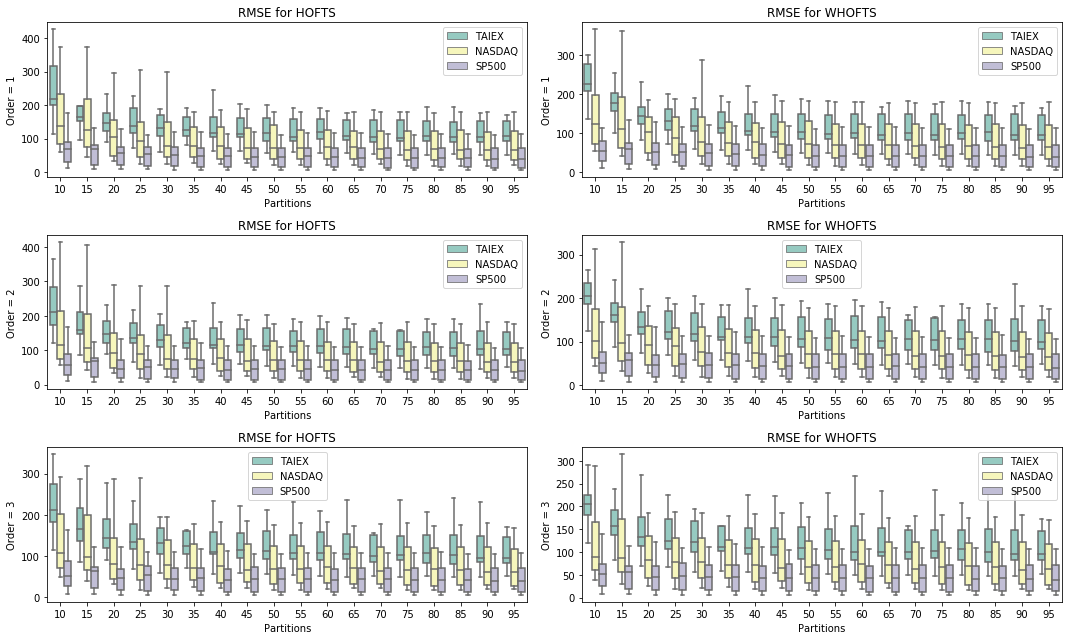
\includegraphics[width=\textwidth, height=12cm]{figures/hofts_gridsearch.png}
    \caption{HOFTS and WHOFTS grid search over hyperparameters $k$ and $\Omega$}
    \label{fig:hofts_gridsearch}
\end{figure}


\begin{figure}[htb]
    \centering
    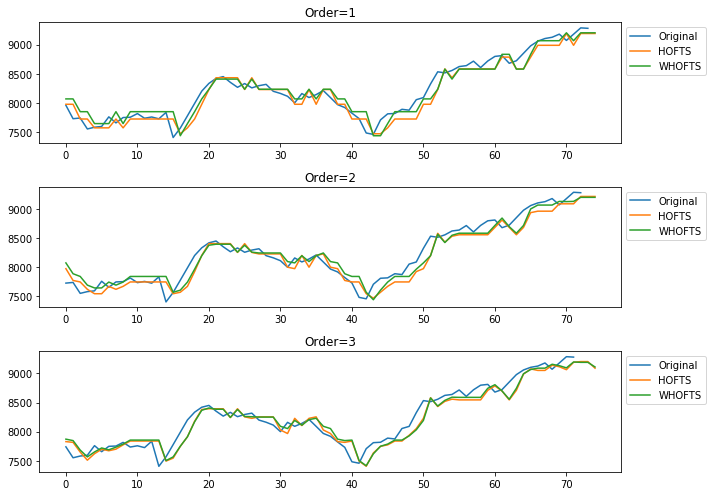
\includegraphics[width=\textwidth]{figures/fts_order.png}
    \caption{The impact of order in forecasting}
    \label{fig:fts_order}
\end{figure}

\begin{figure}[htb]
    \centering
    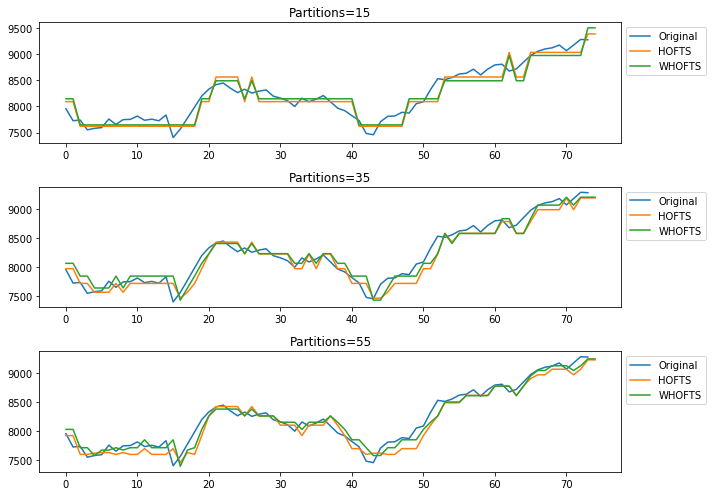
\includegraphics[width=\textwidth]{figures/fts_partitions.png}
    \caption{The impact of partitioning in forecasting}
    \label{fig:fts_partitions}
\end{figure}

%%%%%%%%%%%%%%%%%%%%%%%%%%%%%%%%%%%%%%%%%%%%%%%%%%%%%%%%%%%%%%%%%%%%%%%%%%%%
%%%%%%%%%%%%%%%%%%%%%%%%%%%%%%%%%%%%%%%%%%%%%%%%%%%%%%%%%%%%%%%%%%%%%%%%%%%%
\subsection{Residual Analysis}\index{Residual Analysis}
\label{sec:fts_residual}

The residuals of the models are presented in Figures \ref{fig:hofts_residual} and \ref{fig:whofts_residual} and the Ljung-Box tests for the 3 first lags are presented in Tables \ref{tab:hofts_residuals} and \ref{tab:whofts_residuals}, which show the good fit of model. However, high correlated residuals were detected in some non-stationary sub samples of the datasets, what was also expected since the models are time-invariant. Best performance is expected for time-variant models, capable to adjust its behavior due to changes in data.

\begin{figure}[htb]
    \centering
    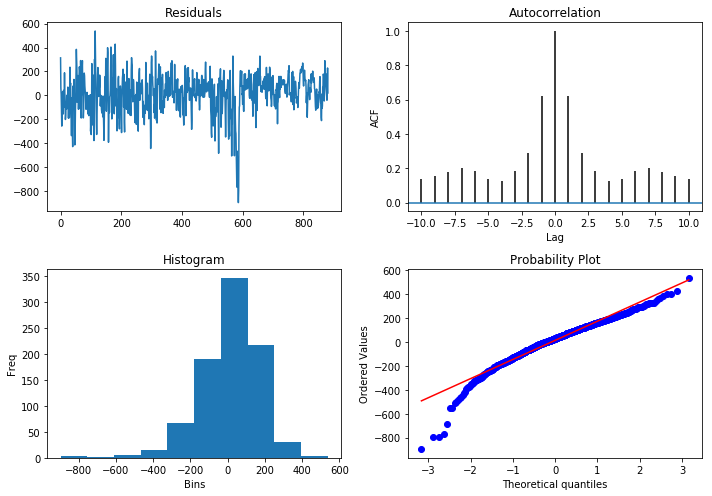
\includegraphics[width=\textwidth,height=7cm]{figures/hofts_residual.png}
    \caption{HOFTS residuals}
    \label{fig:hofts_residual}
\end{figure}

\begin{table}[htb]
    \centering
    \begin{tabular}{|c|c|c|c|c|}
\hline
Lag &   Statistic &  p-Value &  Critical Value &       Result \\ \hline
1 &  341.295085 &      0.0 &        3.841459 &  H0 accepted \\ \hline
2 &  412.500903 &      0.0 &        5.991465 &  H0 accepted \\ \hline
3 &  441.435962 &      0.0 &        7.814728 &  H0 accepted \\ \hline
\end{tabular}
    \caption{Ljung-Box Test for HOFTS residuals}
    \label{tab:hofts_residuals}
\end{table}

\begin{figure}[htb]
    \centering
    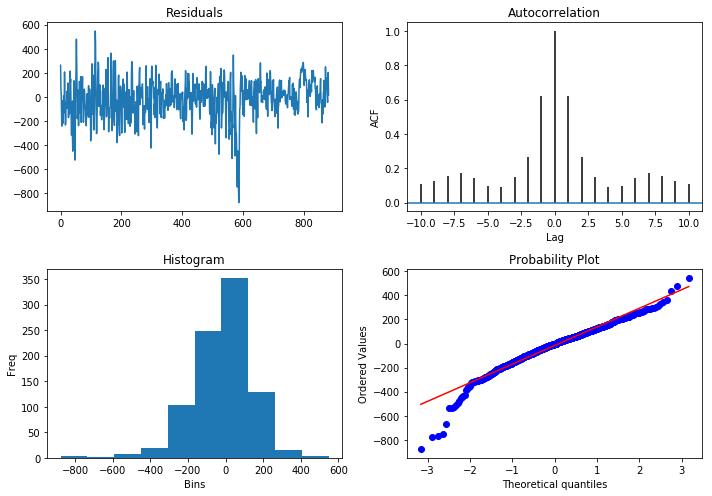
\includegraphics[width=\textwidth,height=7cm]{figures/whofts_residual.png}
    \caption{WHOFTS residuals}
    \label{fig:whofts_residual}
\end{figure}

\begin{table}[htb]
    \centering
    \begin{tabular}{|c|c|c|c|c|}
\hline
Lag &   Statistic &  p-Value &  Critical Value &       Result \\ \hline
1 &  336.838522 &      0.0 &        3.841459 &  H0 accepted \\ \hline
2 &  394.472179 &      0.0 &        5.991465 &  H0 accepted \\ \hline
3 &  411.754344 &      0.0 &        7.814728 &  H0 accepted \\ \hline
\end{tabular}
    \caption{Ljung-Box Test for WHOFTS residuals}
    \label{tab:whofts_residuals}
\end{table}

%%%%%%%%%%%%%%%%%%%%%%%%%%%%%%%%%%%%%%%%%%%%%%%%%%%%%%%%%%%%%%%%%%%%%%%%%%%%
%%%%%%%%%%%%%%%%%%%%%%%%%%%%%%%%%%%%%%%%%%%%%%%%%%%%%%%%%%%%%%%%%%%%%%%%%%%%
\section{Conclusion} 

This chapter provided a brief overview related to the Fuzzy Time Series models. A literature review and some state-of-the-art works related to FTS were presented and summarized in Table \ref{tab:fts_methods}.

The presented methods have some common drawbacks. The matrix-based methods have scalability issues, suffering from the curse of dimensionality. With the rule-based methods, in the forecasting step, just one rule is chosen for computing the result, based on the maximum membership between the input value and all the rules. This causes the loss of ``smoothing'' effect of fuzzy methods, which demands mixing many sets according to their fuzzy membership values. Lastly, these models are point-based forecasters and give no uncertainty measures about their results.  Otherwise, black-box knowledge models eliminate the readability and auditability of the model, and in some cases are not parsimonious. 

To enforce the focus of this research on rule-based FTS methods,  the High Order FTS (HOFTS) and the Weighted High Order FTS (WHOFTS) methods were developed, following a consensus construction from the several approaches present in literature. Computational experiments were employed to assess the point forecasting performance of the methods using financial datasets.

It is necessary to highlight the absence of probabilistic forecasting methods in the Fuzzy Time Series literature. These methods will be discussed in next chapter, where their main features are pointed out and a new method for interval-forecasting with FTS is proposed. 

\begin{center}
    \begin{landscape}
\begin{longtable}[c]{|m{4cm}|c|c|c|c|c|c|c|c|c|m{5cm}|} \hline
\textbf{Reference}   & $n$ & $\Pi$ & $\mu$ & \textbf{Fuzz.} & $\Omega$ & \textbf{Ind.} & \textbf{$\model$}      & \textbf{Transf.} & \textbf{Defuzz.} & \textbf{Application}  \\ \hline \hline
\endhead
%
\cite{song1993fuzzy}      & 1                  & G                  & Tri  & Max                & 1              & H                       & M              & -                        & SM              & Enrollments           \\ \hline
\cite{chen1996forecasting} & 1                  & G                  & Tri  & Max                & 1              & H                       & R               & -                        & SM              & Enrollments           \\ \hline
\cite{Chang1997}           & 1                  & H             & Tri  & All                    & S       & O                    & P          & -                        & -                        & Sales                 \\ \hline
\cite{Song1997}            & 1                  & G                  & Tri  & Max                & 1              & H                       & M              & -                        & -                        & -                     \\ \hline
\cite{Tseng1999}           & 1                  & G                  & Tri  & Max                & S       & O                   & P           & -                        & -                        & Industrial Production \\ \hline
\cite{Song1999}            & 1                  & G                  & Tri  & Max                & S       & H                       & M              & -                        & SM              & -                     \\ \hline
\cite{Chen2000}            & 2                  & G                  & Tri  & Max                & 1              & H                       & M              & -                        & WS            & Temperature           \\ \hline
\cite{huarng2001effective} & 1                  & H             & Tri  & Max                & 1              & H                       & R               & -                        & SM              & Stock Price           \\ \hline
\cite{Chen2002}            & 1                  & G                  & Tri  & Max                & 5              & H                       & R              & -                        & SM              & Enrollments           \\ \hline
\cite{Huarng2004}          & 1                  & H             & Tri  & Max                & 1              & H                       & R               & -                        & SM              & Stock Price           \\ \hline
\cite{yu2005weighted}              & 1                  & G                  & Tri  & Max                & 1              & H                       & WR      & -                        & WS            & Stock Price           \\ \hline
\cite{Huarng2006}          & 1                  & G                  & Tri  & Max                & 1              & BP                              & NN                 & -                        & SM              & Stock Price           \\ \hline
\cite{Chen2006a}           & 1                  & MH         & Tri  & Max                & 3              & H                       & M              & -                        & SM              & Enrollments           \\ \hline
\cite{Lee2006}             & 4                  & G                  & -           & Max                & 1              & H                       & R               & -                        & SM              & Stock Price           \\ \hline
\cite{Cheng2006a}          & 1                  & E               & Trap & Max                & 1              & H                       & M              & -                        & SM              & Project Cost          \\ \hline
\cite{Cheng2008}          & 1                  & E               & Trap & Max                & 1              & H                       & M              & -                        & WS            & Outpatient visits     \\ \hline
\cite{Cheng2008a}           & 1                  & G                  & -           & -                      & 1              & H                       & WR      & D, AE           & WS            & Stock Price           \\ \hline
\cite{Jilani2008a}         & 6                  & G                  & Tri  & Max                & 4              & H                       & M              & -                        & WS            & -                     \\ \hline
\cite{Li2008b}             & 2                  & C            & FCM         & All                    & 2              & H                       & R                & -                        & SM              & Temperature           \\ \hline
\cite{Davari2009}          & 2                  & MH         & Tri  & Max                & 1              & H                       & M              & -                        & WS            & Enrollments           \\ \hline
\cite{Kuo2009}             & 1                  & MH         & -           & -                      & ?              & MH                             & WR      & -                        & ?                        & Enrollments           \\ \hline
\cite{Egrioglu2009}        & 2                  & G                  & Trap & All                    & 3              & BP                              & NN                 & -                        & SM              & Accident              \\ \hline
\cite{Hsu2010}             & 2                  & MH         & -           & Max                & 1              & H                       & R               & -                        & SM              & Temperature           \\ \hline
\cite{Chen2011}            & 2                  & -                     & -           & -                      & ?              & H                       & WR      & D                     & -                        & Stock Price           \\ \hline
\cite{Huang2011}           & 1                  & MH   & Tri  & Max                & 3              & H                       & R               & AE                 & WS            & Enrollments           \\ \hline
\cite{Lee2011}             & 1                  & G                  & -           & -                      & S       & H                       & WR      & D                     & -                        & Stock Price           \\ \hline
\cite{ismail2011enrollment}          & 1                  & G                  & -           & Max                & 1              & H                       & WR      & -                        & WS            & Enrollments           \\ \hline
\cite{Cheng2012}           & 1                  & -                     & -           & -                      & ?              & H                       & WR      & ?                        & -                        & -                     \\ \hline
\cite{Enayatifar2013}      & 1                  & MH         & -           & -                      & 3              & MH                   & WR      & AE                 & -                        & Energy Load           \\ \hline
\cite{Lee2013}             & 1                  & G                  & -           & -                      & 1              & H                       & WR      & BC                  & WS            & Stock Price           \\ \hline
\cite{Chen2014}            & 1                  & E               & -           & -                      & 2              & H                       & WR      & ?                        & -                        & Stock Price           \\ \hline
\cite{Sadaei2014a}          & 1                  & -                     & -           & Max                & 1              & H                       & WR      & ROI, AE            & WS            & Stock Price           \\ \hline
\cite{Askari2015}          & 3                  & C            & FCM         & All                    & 1              & H                       & P & -                        & WS            & Stock Price           \\ \hline
\cite{Bas2015}             & 1                  & C            & FCM         & All                    & 1              & MH                             & NN                 & -                        & WS            & Stock Price           \\ \hline
\cite{Cai2015}             & 1                  & MHs        & trmf        & All                    & 1              & H                       & WR      & -                        & WS            & Stock Price           \\ \hline
\cite{Chen2015a}           & 2                  & G                  & Tri  & Max                & 2              & H                       & R               & -                        & WS            & Stock Price           \\ \hline
\cite{Ismail2015}          & 1                  & Q              & -           & -                      & 1              & H                       & M              & -                        & SM              & Energy Load           \\ \hline
\cite{Sun2015}             & 3                  & C            & FCM         & All                    & 1              & H                       & R                & -                        & WS            & Stock Price           \\ \hline
\cite{Singh2015}           & 3                  & G                  & -           & Max                & 1              & BP                             & NN                 & AE             & WS            & Stock price           \\ \hline
\cite{Rubio2016}           & 1                  & H             & Trap & All                    & 1              & H                       & M              & -                        & WS            & Portfolio returns     \\ \hline
\cite{Sadaei2016}          & 1                  & G                  & Tri  & Max                & 1              & H                       & R               & D, AE           & SM              & Stock Price           \\ \hline
\cite{Talarposhti2016a}    & 1                  & MH         & Tri  & Max                & 1              & H                       & P  & -                        & WS            & Stock Price           \\ \hline
\cite{Ye2016}              & 1                  & G                  & Tri  & AC              & 3              & MH                         & M              & ROC, AE            & WS            & Sock price            \\ \hline
\cite{Lee2017}             & 1                  & G                  & Tri  & Max                & 3              & H                     & R               & -                        & WS            & Enrollments           \\ \hline
\cite{Yang2017}            & 3                  & CS            & Tri  & Max                & 1              & H                       & R               & EMD, AE            & SM              & Wind Speed            \\ \hline
\cite{Yolcu2017}           & 1                  & C            & FCM         & All                    & 1              & MH                             & MLP                 & -                        & WS            & Sock price            \\ \hline
\cite{Bose2017}            & 1                  & C            & Tri  & -                      & 3              & H                       & R                & AE                 & WS            & -                     \\ \hline
\cite{CarvalhoJr2017}      & 1                  & G                  & Tri  & AC              & 1              & H                       & R               & -                        & SM              & Stock price           \\ \hline
\cite{Jiang2017}           & 1                  & MH         & Tri  & Max                & 3              & H                       & WR      & -                        & WS            & Stock price           \\ \hline
\cite{Saberi2017}          & 1                  & C            & fefts       & All                    & 1              & H                       & M              & -                        & WS            & -                     \\ \hline
\cite{Sadaei2017}          & 1                  & MH         & Tri  & Max                & *              & O                         & P      & -                        & ?                        & Energy Load           \\ \hline
\cite{Severiano2017a}      & 1                  & G                  & Tri  & All                    & 3              & H                       & R               & -                        & SM              & Energy Load           \\ \hline
\cite{Bas2018}             & 1                  & C            & FCM         & All                    & 1              & P                             & NN               & -                        & WS            & Stock price           \\ \hline
\cite{Guney2018}           & 1                  & G                  & Tri  & Max                & 2              & H                       & MC        & -                        & WS            & -                     \\ \hline
\cite{Cheng2018}           & 1                  & H             & Trap & Max                & 3              & A                         & R                & -                        & WS            & Stock price           \\ \hline
\cite{Dincer2018}          & 1                  & C            & -           & Max                & 1              & H                       & M              & -                        & SM              & Air pollution         \\ \hline
\cite{Yang2018}            & 5                  & MH         & Trap & Max                &                & MH                   & P  & EMD                      & WS            & Stock price           \\ \hline
\cite{Yang2018}            & 5                  & C            & -           & -                      & 2              & RG                      & FCM                 & WV                 & WS            & -                     \\ \hline
\cite{Tran2018}            & 3                  & C            & -           & All                    & 1              & BP                            & NN                & N            & WS            & -                     \\ \hline
\cite{Zhang2018}           & 4                  & H                & FCM         & -                      & 1              & BP                             & NN                 & -                        & WS            & Stock price           \\ \hline
\cite{Zhang2018a}          & 2                  & MH         & Tri  & Max                & 2              & H                       & R               & -                        & SM              & Stock price           \\ \hline
\cite{Chen2019a}            & 1                  & G                  & Trap & Max                & 1              & H                       & M              & -                        & WS            & Flood \\  \hline
\cite{Sadaei2019}            & 1                  & G                  & Tri & Max                &  *              & BP                       & NN              & -                        & WS            & Energy Load \\  \hline
\multicolumn{11}{l}{$\mathbf{n}$\textbf{ - Number of variables}} \\
\multicolumn{11}{p{20cm}}{$\mathbf{\Pi}$\textbf{ - Partitioning method}: G - Grid, H - Heuristic, MH - Metaheuristic, CS - Chi-Square, E - Entropy, Q - Quartile} \\
\multicolumn{11}{p{20cm}}{$\mathbf{\mu}$\textbf{ - Membership function}: Tri - Triangular, Trap - Trapezoidal, FCM - Fuzzy C-Means} \\
\multicolumn{11}{p{20cm}}{\textbf{Fuzz - Fuzzyfication method}: Max - Maximum membership, All - All memberships, AC - alpha-cut} \\
\multicolumn{11}{l}{$\mathbf{\Omega}$\textbf{  - Order}} \\
\multicolumn{11}{p{20cm}}{\textbf{Ind. - Knowledge induction method}: H - Heuristic, MH - Metaheuristic, BP - Backpropagation, O - Optimization, RG - Regression analysis, AP - Apriori} \\
\multicolumn{11}{p{20cm}}{$\mathbf{\model}$\textbf{ - Knowledge model}: M - Matrix, R - Rules, WR - Weighted Rules, NN - Neural Network, FCM - Fuzzy Cognitive Map, P - Polynomial, MC - Markov Chain} \\
\multicolumn{11}{p{20cm}}{\textbf{Transf - Transformations}: A - Adaptive expectation; B - Box-Cox;  D - Differentiation; R - ROI, N - Normalization} \\ \hline
\caption{Summary of the most relevant FTS methods}
\label{tab:fts_methods}\\
\end{longtable}
\end{landscape}
\end{center}

\chapter[Probabilistic Forecasting]{Probabilistic Forecasting} 
\label{chap:review_probforecasting} \index{Probabilistic Forecasting}
\label{chap:prob}

\newepigraph{Uncertainty is an uncomfortable position. But certainty is an absurd one.}
{Voltaire}

This chapter briefly discusses the uncertainty of point forecasts to introduce the interval and probabilistic forecasting and review the related literature, pointing the most representative methods of each type. To fill the lacks on FTS literature, two new FTS methods are proposed for representing the fuzzy uncertainty, the Interval FTS and the Ensemble FTS.

Previously on this work it was presented the two main uncertainties kinds, the epistemic and the ontological, that imposes limits to predictability of forecasting methods. The origin of these limitations, according  to \cite{Krzysztofowicz2001} are ``theoretical, technological and budgetary''. In his seminal work, \cite{Lorenz1963} prove that even some deterministic systems decay to chaotic behavior due to minimal fluctuations on their start conditions. This effect put limits on the predictability of these systems and the probabilistic forecasts are the ideal way to deal with these limitations. 

Also \cite{Makridakis2010} poses that ``statistical regularity does not equal predictability'' on his study about the common sources of unreliability on forecasts. In \cite{Makridakis2016} the authors split the forecasting uncertainty in four categories: Known Knowns (normal and usual conditions), Unknown Knowns (uncertainty known but not covered by models), Known Unknowns (rare, unusual and special conditions) and Unknown Unknowns (unexpected and unpredictable conditions, also called by black swans). This survey also discuss the specific sources of uncertainty at several forecasting areas as natural (weather, earthquakes, volcanoes, tsunamis, floods) and social (economical and demographical) events.

In this context emerged the probabilistic forecasting approaches, defined by \cite{Gneiting2014b} as ``the form of a predictive probability distribution over future quantities or events of interest". This definition enclose two main forecasting types: intervals and probability distributions. Their importance appears as we analyze the impact of the intrinsic uncertainty on the point forecasts, and how this uncertainty grows as the forecasting horizon increases. 

In following sections are presented a short review of uncertainties in forecasting models, starting with the limitations of point forecasts on Section \ref{sec:prob_point}, and its accuracy measures. On Section \ref{sec:prob_interval}, the most known interval forecasting methods and its evaluation measures are presented. On Section \ref{sec:ifts} new FTS methods are proposed to produce prediction intervals representing the fuzzy uncertainty. On Section \ref{sec:prob_distribution} the major approaches for probabilistic forecasting and its accuracy measures are discussed. On Section \ref{sec:ensemblefts} a new FTS method is proposed to produce interval and probabilistic forecastings. On Section \ref{sec:prob_experiments}, computational experiments are performed to assess the accuracy and computational performance of the proposed methods and finally, on Section \ref{sec:prob_conclusion}, the conclusions are pointed. 

%%%%%%%%%%%%%%%%%%%%%%%%%%%%%%%%%%%%%%%%%%%%%%%%%%%%
%
%%%%%%%%%%%%%%%%%%%%%%%%%%%%%%%%%%%%%%%%%%%%%%%%%%%%
\section{The Point Forecast Limitations}
\label{sec:prob_point}

\index{Deterministic Forecast}\index{Point Forecasts}
\index{Conditional Expectation}\index{Conditional Variance}

Point forecasts, are usually defined by the conditional expectation $\mathbb{E}[y(t+1)|y(t),y(t-1),...]$ which in turn minimize a cost function that represents the accuracy error, as the mean squared error on Equation \ref{eqn:rmse}. In statistics textbooks, as \cite{Kay2006}, this conditional expectation is  known to be the best linear and non-linear estimator for $y(t+1)$ given the lagged values $y(t),y(t-1),...$. But for the layman this optimality may be misunderstood as the absence of error and not the normality of error terms $\epsilon$, defined as the white noise $\epsilon \sim \mathcal{N}(0,1)$. These deterministic forecasts, according to \cite{Krzysztofowicz2001}, create a ``illusion of certainty in a user's mind''. 

It is expected that the conditional variance $Var[y(t+1)|y(t),y(t-1),...]$ be presented with the conditional expectation to represent the uncertainty around this result, but this is not really usual as is need to be. Even this common statistical approach is not enough to capture all uncertainty of an estimate and \cite{Makridakis2009} point out that error variance may not be known, constant or finite.

\index{Many Steps Ahead Forecasts}
When dealing with the many steps ahead forecasts, where $H \in \mathbb{N}^+$ is the forecasting horizon, it is necessary to consider the propagation of errors. \cite{Leutbecher2008} address this problem in the context of weather forecasting, where the major source of uncertainty is inaccuracy on initial parameters estimation. Also \cite{Smith2001} states that ``the question of prediction then turns to how to best quantify the dynamics of uncertainty'' of propagating errors.

Many steps ahead forecasts can be calculated in several ways, for instance fitting a specific model for each $h = 1\ldots H$ step, as $\mathbb{E}[y(t+h)|y(t),y(t-1),\ldots]$, or iterating the model. If the time series is stationary, long runs ($h \rightarrow \infty$) of the conditional mean will fatally fall on unconditional mean.



%%%%%%%%%%%%%%%%%%%%%%%%%%%%%%%%%%%%%%%%%%%%%%%%%%%%
%
%%%%%%%%%%%%%%%%%%%%%%%%%%%%%%%%%%%%%%%%%%%%%%%%%%%%
\section{Interval Forecasts}
\label{sec:prob_interval}\index{Interval Forecasts}

\index{Confidence Interval}\index{Prediction Interval}
The simplest evolution of point forecasts are the interval forecasts, that represent and incorporate uncertainty \cite{Hansen2006}. At first sight interval forecasts may be confused with confidence intervals because they share the same structure, but they are slightly different things. Both are defined with respect to an unknown value $y(t+1)$ as an interval $\interval$  with $\alpha$ confidence level to contain the real value of $y(t+1)$. The probability of $\intvl$ to contain $y(t+1)$ is given by $P(\underline{l} \leq y(t+1) \leq \overline{u}) = 1 - \alpha$.

\index{Prediction Intervals}

Confidence intervals deal with fixed (but unknown) estimates. Prediction intervals instead, as proposed by \cite{Chatfield1993}, are an ``estimate of an (unknown) future value that can be regarded as a random variable at the time the forecast is made. This involves a different sort of probability statement to a confidence interval as discussed''. Traditional approaches for this kind of forecasting include the parametric methods as studied in  \cite{Chatfield1993}. These methods use strong statistical assumptions about the data that can make it less useful where data is not conforming.

The confidence level $\alpha \in (0,1)$ is then a way to determine a symmetric inter-quantile interval $[\alpha, 1-\alpha]$ for some forecasted value of interest. If a cumulative probability distribution $F:U \rightarrow [0,1]$ finds the probability $F(x) =  P(X \leq x)$, the quantile function $Q:(0,1) \rightarrow U$ performs the opposite process: $Q(\tau) = \min_x\{ x \in U \ |\ \tau < F(x) \}$ where $\tau \in (0,1)$ is a quantile.

\index{Mean-variance prediction intervals}\index{Error variance exponential smoothing}

\cite{Chatfield2001} proposed a simple method for creating $\alpha$-level prediction intervals for generic forecasting models, the called mean-variance model. From the point forecast $\mu = \mathbb{E}[Y_{t+1}|Y_t,Y_{t-1},...]$ with the variance of the residuals $\sigma_\epsilon = \sqrt{VAR[\epsilon]}$ by assuming that these residuals as $\epsilon \sim \mathcal{N}(0,1)$. The prediction interval is calculated by $I = [\mu - z_{\alpha/2}\sigma_\epsilon\ ,\ \mu + z_{\alpha/2}\sigma_\epsilon]$ and $z_{\alpha/2} = \Phi((1- \alpha)/2)$ is the standard normal distribution function. On Figure \ref{fig:arima} is represented an example of ARIMA(2,0,0) process where the prediction intervals where calculated with the previous model, for $\alpha \in \{0.05,0.25\}$. 

For $H$-steps ahead, the variance $\sigma_\epsilon^h$ can be estimated from the 1-step ahead variance $\sigma_\epsilon^1$ through exponential smoothing by $\sigma_\epsilon^h = (1 + h\beta)\sigma_\epsilon^1$, for some smoothing vale $\beta \in (0,1)$. Besides its simplicity, the main drawback of this method is the parametric and homoskedastic assumption over the residuals distribution. On Figure \ref{fig:arima} is represented an example of ARMA(2,0,0) process where the prediction intervals for 7 steps ahead where calculated with the exponential smoothing, for $\alpha \in \{0.05,0.25\}$ and $\beta = 0.5$. But \cite{Chatfield2001} warns that mean-variance model is an generic approximation and do not replace prediction interval models specifically developed from the statistical methods and their error distribution assumptions. 

\index{Quantile Auto Regression}\index{QAR}\index{Pinball Loss Function}

The main probabilistic approach for interval forecasting is the Quantile Auto Regression - QAR proposed by \cite{Koenker2006} based on the Quantile Regression \cite{Koenker2001}. The QAR estimate a conditional quantile function in Equation \ref{eqn:qar}, where $\hat{y(t)}$ is the estimated quantile value, $\tau$ is the quantile level, $\theta$ are the fitted coefficients for the $y(i)$ lagged values and $\rho_\tau(u)$ is the Pinball Loss Function, defined on Equation \ref{eqn:pinball}, where $\mathbf{1}(x) = \{ 1$ if $x \geq 0$ or $0$ if $x < 0\}$. Quantile Regression approaches have been used at many application fields, for instance energy load forecasting [\cite{Liu2015}, \cite{Hong2016}, \cite{Hong2016a}] and wind forecasting \cite{Pinson2006}.

\begin{equation}
Q_{y(t)}(\tau | y(t-1),\ldots) = \min_\theta \sum_{i=1}^n \rho_\tau (y(t) - y(i)\theta)    
\label{eqn:qar}
\end{equation}

\begin{equation}
    \rho_\tau(u) = u(\tau - \mathbf{1}(u < 0))
    \label{eqn:pinball}
\end{equation}

Each QAR model is fitted for a specific $\tau$, so for a certain $\alpha$ two QAR models are necessary. The independence of quantiles  also allows to create asymmetric inter quantile intervals, if needed. On Figure \ref{fig:qar} is represented an example of QAR(2) for $\tau \in \{0.05,0.25,0.75,0.95\}$, equivalent for $\alpha \in \{0.05,0.25\}$.  The same principle is applied for $H$-steps ahead forecasts, it is needed to fit an specific model for each step ahead. This mean, for example, that will be required to fit 10 models to generate prediction intervals for 5 steps ahead. This approach is not very flexible and difficult their adoption for final users.

\begin{figure*}
\begin{center}
\begin{subfloat}[ARIMA(2,0,0) prediction intervals]{
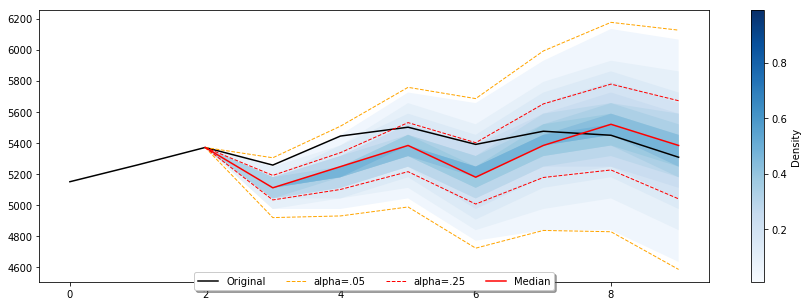
\includegraphics[width=6in,height=1.8in]{figures/arima.png}
\label{fig:arima}}
\end{subfloat}

\begin{subfloat}[Quantile Auto Regression - QAR]{
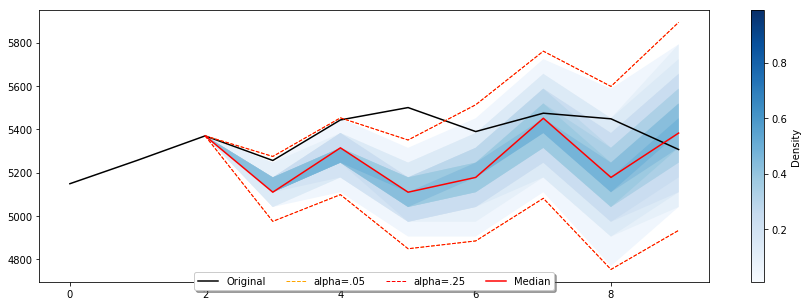
\includegraphics[width=6in,height=1.8in]{figures/qar.png}
\label{fig:qar}}
\end{subfloat}

\begin{subfloat}[Bayesian Structural Time Series - BSTS]{
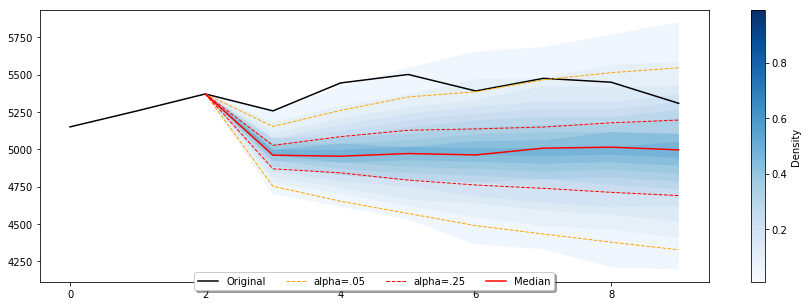
\includegraphics[width=6in,height=1.8in]{figures/bsts.png}
\label{fig:bsts}}
\end{subfloat}

\begin{subfloat}[k-Nearest Neighbors with Kernel Density Estimation - kNN/KDE]{
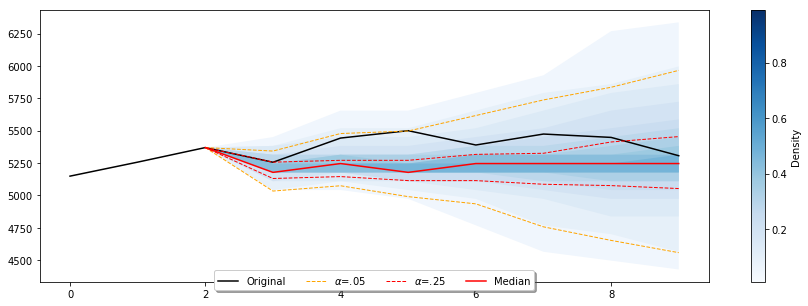
\includegraphics[width=6in,height=1.8in]{figures/knn.png}
\label{fig:knn}}
\end{subfloat}

\caption{Prediction Intervals}
\label{fig:prediction_intervals}
\end{center}
\end{figure*}

The Pinball Loss Function $\rho_\tau(u)$ is a general measurement to quantile approximation and \cite{Steinwart2011} also use it with Support Vector Machines to perform quantile regressions. \cite{Wan2014} use it with Extreme Learning Machines to fit quantile regression models. Other approaches are available in \cite{Takeuchi2006} for non parametric quantile estimation,  \cite{Taylor2007} proposes a Exponentially Weighted Quantile Regression and \cite{Hansen2006}, which proposes a semi-parametric k-step ahead approach for quantile estimation. \cite{Gardner1998} proposed a simple non parametric method for computing intervals based on the Chebyshev Inequality $P(|(Y-\mu)/\sigma|\geq \epsilon) \leq 1/\epsilon$ where $\mu$ is the mean, $\sigma$ the standard deviation and $\epsilon$ will be estimated value, such as the forecasted interval is $[y(t+1) - \epsilon, y(t+1) + \epsilon]$.

%%%%%%%%%%%%%%%%%%%%%%%%%%%%%%%%%%%%%%%%%%%%%%%%%%%%
%
%%%%%%%%%%%%%%%%%%%%%%%%%%%%%%%%%%%%%%%%%%%%%%%%%%%%
\subsection{Accuracy Measures for Interval Forecasts}
\label{sec:prob_interval_measures}
\index{Accuracy Measures}\index{Interval Forecasting Accuracy Measures}

In a wide sense the point forecasting accuracy measures can be used to assess the interval forecasts. This is possible using the midpoint of the prediction interval, if the interval is based on $\alpha$-levels or symmetric quantiles. But, by far, this is not the ideal way to measure the interval accuracy, once several aspects of prediction intervals are neglected by single point measures.

Some the main aspects to be considered when evaluating prediction intervals are the \textit{coverage rate}, \textit{calibration} and \textit{sharpness}, as proposed in \cite{Gneiting2007} and \cite{Pinson2006}. The \textit{coverage} refers to the statistical consistency between the forecasts and the observations, and measures which proportion of the observations are inside the interval. This can be done by an Indicator Function, developed by \cite{Christoffersen1998}, as shown in Equation \ref{eqn:indicator}. Given a forecasting interval $\interval, u,l \in U$ and the real value $y\in Y$, the value of an indicator function $\mathbf{1}(\intvl(t),y(t))$ verifies if $y(t)$ is covered by $\intvl(t)$ or not.

\begin{equation}
\mathbf{1}(\intvl(t),y(t)) = \left\{ \begin{array}{cl}
1 & \text{if }y(t) \in \intvl(t) \\
0 & \text{if }y(t) \ni \intvl(t) 
\end{array} \right.
\label{eqn:indicator}
\end{equation}

\index{Coverage Rate}\index{Interval metrics}

The \textit{coverage rate} is the average value of indicator function between forecasted intervals and the real values, in which the ideal value is 1. The coverage rate is shown at Equation \eqref{eqn:coverage} where $y(t) \in Y$ are the real values and $\intvl(t) \in \intvl$ are the predicted intervals for these values.

\begin{equation}
C(Y,\intvl) = T^{-1}\sum_{t = 1 }^T \mathbf{1}(\intvl(t),y(t))
\label{eqn:coverage}
\end{equation}

\index{Sharpness}\index{Resolution}\index{Interval metrics}

The property of \textit{sharpness} and \textit{resolution} refers to the concentration of the predictive distribution, or how wide and variable are the intervals and refers uniquely to the forecasts. \textit{Sharpness}, presented in Equation \eqref{eqn:sharpnes}, is the average size of the intervals and \textit{resolution}, presented in the equation \eqref{eqn:resolution}, is the variability of the intervals.   

\begin{equation}
\overline{\delta(\intvl)} = T^{-1}\sum_{t=1}^{T} \delta(\intvl(t)) =  T^{-1}\sum_{t=1}^T \overline{u_t} - \underline{l_t}
\label{eqn:sharpnes}
\end{equation}
\begin{equation}
\sigma(\intvl) = T^{-1}\sum_{t=1}^T | \delta(\intvl(t)) - \overline{\delta(\intvl)}|
\label{eqn:resolution}
\end{equation}

While small values of $\overline{\delta(\intvl)}$ are desirable, meaning a compact interval, wide values of $\sigma(\intvl)$ are best, meaning the capability of the model to adapt the length of interval with the increase of uncertainty. There are no absolute reference values for sharpness and resolution, which depend on the statistical properties of the data. Empirically, when the sharpness is reduced to make the intervals thinner and more precise, the risk of reducing the coverage increase, and that's why the resolution is important. 

\index{Pinball Loss Function}\index{Pinball Score}\index{Interval metrics}

\cite{Steinwart2011} proposed the use of Pinball Loss Function - $\rho_\tau(u)$, defined in equation \ref{eqn:pinball} where $u = y(t) - \hat{y}(t)$, to indicate the proximity of a forecast $\hat{Y}$ with a certain $\tau$ quantile of the true value $Y$. As a loss function, the minor value of $\rho_\tau$ indicates the closest forecast to quantile $\tau$. The Pinball Score $\rho_\tau^S$ is defined as the mean $\rho_\tau$ for a set true values $y(t)$ and forecasts $\hat{y}(t)$, listed on Equation \ref{eqn:pinball_score}. At this research were chosen the quantiles $\tau = \{0.05, 0.25, 0.75, 0.95\}$ for testing the intervals, where the lower quantiles were compared with the interval lower bound and the upper quantiles with the interval upper bounds.

\begin{equation}
\rho_\tau^S(Y,\hat{Y}) = \frac{1}{T}\sum_{t=1}^T \rho_\tau(y(t) - \hat{y}(t))
\label{eqn:pinball_score}
\end{equation}

However, using three separate metrics make the analysis of interval forecasters more complex. The most common option in these cases is the Winkler score \cite{winklerscore}, which encompasses the three characteristics in only one measure. Given a target value $y$ and a prediction interval $\interval$ with nominal probability $(1 - \alpha)$, the Winkler Score (WS) is defined by  \eqref{eqn:winkler}, where $\delta = \overline{u} - \underline{l}$. The score value is the interval width, but it increases when the target value is not covered by the interval and the penalty is proportional to the error given the nominal probability. Lower values therefore represent better prediction intervals. The mean score is defined by Equation \eqref{eqn:mean_winkler}, where $T$ is the sample size.

\begin{equation}
WS(\alpha, y(t), \intvl(t)) = \left\{ \begin{array}{ccl}
\delta & if & \underline{l} \leq y \leq \overline{u} \\
\delta + 2(\underline{l} - y)/\alpha & if & y < \underline{l}  \\
\delta + 2(y - \overline{u})/\alpha & if & \overline{u} < y   
\end{array} \right.
\label{eqn:winkler}
\end{equation}

\begin{equation}
\overline{WS(\alpha, Y, \intvl)} = T^{-1} \sum_{t=1}^T S(\alpha, y(t),\intvl(t))
\label{eqn:mean_winkler}
\end{equation}

All revised interval forecasting methods are based on non-FTS methods and this is a lack on FTS literature. In next section a method for quantify the bounds of fuzzy uncertainty is proposed.

\index{Interval Fuzzy Time Series}\index{$[\mathbb{I}]$FTS}

%%%%%%%%%%%%%%%%%%%%%%%%%%%%%%%%%%%%%%%%%%%%%%%%%%%%
%
%%%%%%%%%%%%%%%%%%%%%%%%%%%%%%%%%%%%%%%%%%%%%%%%%%%%
\section{The Interval Fuzzy Time Series  - $\ifts$}
\label{sec:ifts}

It was already discussed in Section \ref{sec:fts_partitions} the impact of the number of partitions $k$ on the accuracy of a FTS model. Also, on Section \ref{sec:fts_defuzzyfication} it is possible to note that on the deffuzification process only the midpoint of each fuzzy set is taken in account. This lead to the following question: what is the impact of the fuzzy set bounds - the empirical uncertainty - on the final forecasting uncertainty? 

The objective of this section is to propose a simple, fast and effective method to deal with fuzzy empirical uncertainty, combining the flexibility of the FTS models with the properties of Interval Forecasts without the need to resort to parametric methods or optimization techniques as in quantile estimation methods. The importance of this is, for example, when the method is used in a high volume data or on a fast stream with concept drifts, which demands the model to be frequently updated.

The Interval Fuzzy Time Series Model ($\ifts$) aims to produce a prediction interval that represents the empirical uncertainty caused by the number of partitions $k$ and the fuzzy sets bounds, but without any probabilistic meaning. The method $\ifts$ is a time invariant, rule based and high-order method that just  introduces a new deffuzyfication type on forecasting procedure, without modifying the training method and, because of this, can be applied to every conventional FTS method.  

The model training procedure is the same of HOFTS presented in Section \ref{sec:fts_training_procedure} and aims to construct the FLRG rule base $\model$. The prediction intervals are based on the mean interval of the $RHS$ fuzzy sets on each FLRG weighted by their fuzzy membership in relation to input value.

In the following section will be presented the forecasting method of $\ifts$ that extends the HOFTS forecasting method, presented in Section \ref{sec:fts_forecasting_procedure}, changing its output from the crisp value $\estimate$ to the prediction interval $\intvl(t+1)$.

%%%%%%%%%%%%%%%%%%%%%%%%%%%%%%%%%%%%%%%%%%%%%%%%%%%%
%
%%%%%%%%%%%%%%%%%%%%%%%%%%%%%%%%%%%%%%%%%%%%%%%%%%%%
\subsection{Forecasting Procedure} 
\label{sec:ifts_forecasting_procedure}

\begin{enumerate}
\item [Step 1] \textit{Fuzzyfication}: Compute the membership grade $\mu_{ti}$ for each $y(t) \in Y$ where $t \in L$ and each fuzzy set $A_i \in \Tilde{A}$, such that $\mu_{ti} = \mu_{A_i}(y(t))$. 
\item [Step 2] \textit{Rule matching}: Select the $K$ rules where all fuzzy sets $A_i$ on the LHS have $\mu_{ti} > \alpha$; The rule fuzzy membership grade is shown below, using the minimum function as T-norm.
\begin{equation}
    \mu_j = \bigcap_{t\in L\; i \in \Tilde{A}} \mu_{ti}
\end{equation}

\item [Step 3] \textit{Interval Defuzzyfication}:
\begin{enumerate}
\item \textit{Rule intervals}: Each chosen rule $j$ will generate a interval $\mathbb{I}^j = [\underline{\mathbb{I}^j_{min}}, \overline{\mathbb{I}^j_{max}}]$ where $\mathbb{I}^j_{min}$ is the minimum lower bound of all RHS fuzzy sets of the rule $j$ and $\mathbb{I}^j_{max}$ is the maximum upper bound of RHS fuzzy sets of rule $j$;
\begin{equation}
\begin{array}{lcr}
\mathbb{I}^i_{min} & = & min( A_1, ..., A_k ) \\
\mathbb{I}^i_{max} & = & max( A_1, ..., A_k ) \\ 
& & A_1, ..., A_k \in RHS 
\end{array}
\label{eqn:iminimax}
\end{equation}

\item \textit{Final Prediction Interval}: The final forecast interval $\mathbb{I}(t+1)$ is calculated as the sum of the rules intervals weighted by the membership value of each rule, as showed in Equation \ref{eqn:ifts}
\begin{equation}
\mathbb{I}(t+1) = \frac{\sum_{j \in A} \mu_i \mathbb{I}^j}{\sum_{j \in A} \mu_j} = \frac{\sum_{j \in A} [\mu_j\underline{\mathbb{I}^j_{min}} , \mu_j\overline{\mathbb{I}^j_{max}}] }{\sum_{j \in A} \mu_j}
\label{eqn:ifts}
\end{equation}
\end{enumerate}
\item[Step 5] \textit{Many steps ahead forecast}:If the forecasting horizon is $H > 1$, define $\intvl_H = \{\intvl(t+1)\}$ as the set of intervals and repeat the below steps for each $h=2..H$, otherwise return  $\intvl(t+1)$.
\begin{enumerate}
    \item[a)]  Given $\intvl(t+h-1)= [\underline{l},\overline{u}]$, call recursively the forecasting method, such that $\intvl_l = forecast(\underline{l})$ and $\intvl_u = forecast(\underline{u})$. The interval $\intvl(t+h)$ is given by:
    \begin{equation}
        \intvl(t+h)= [\underline{min(\intvl_l)},\overline{max(\intvl_u)}]
    \end{equation}
    \item[b)] Append $\intvl(t+h)$ to $\intvl_H$ and if $h = H$ then return $\intvl_H$.
\end{enumerate}
\end{enumerate}

The generated interval $\intvl(t+1)$ is bounded by a composition of the fuzzy sets bounds on the FLRG's which have some membership with the input value $y(t)$ and is expected to contain the true value $\estimate$. A sample of the method performance, for one and many steps ahead, can be seen in Figures \ref{fig:ifts_sample_onestep} and \ref{fig:ifts_sample_manystep}. In next section a weighted version of $\ifts$ is presented. 

\begin{figure}[htb]
    \centering
    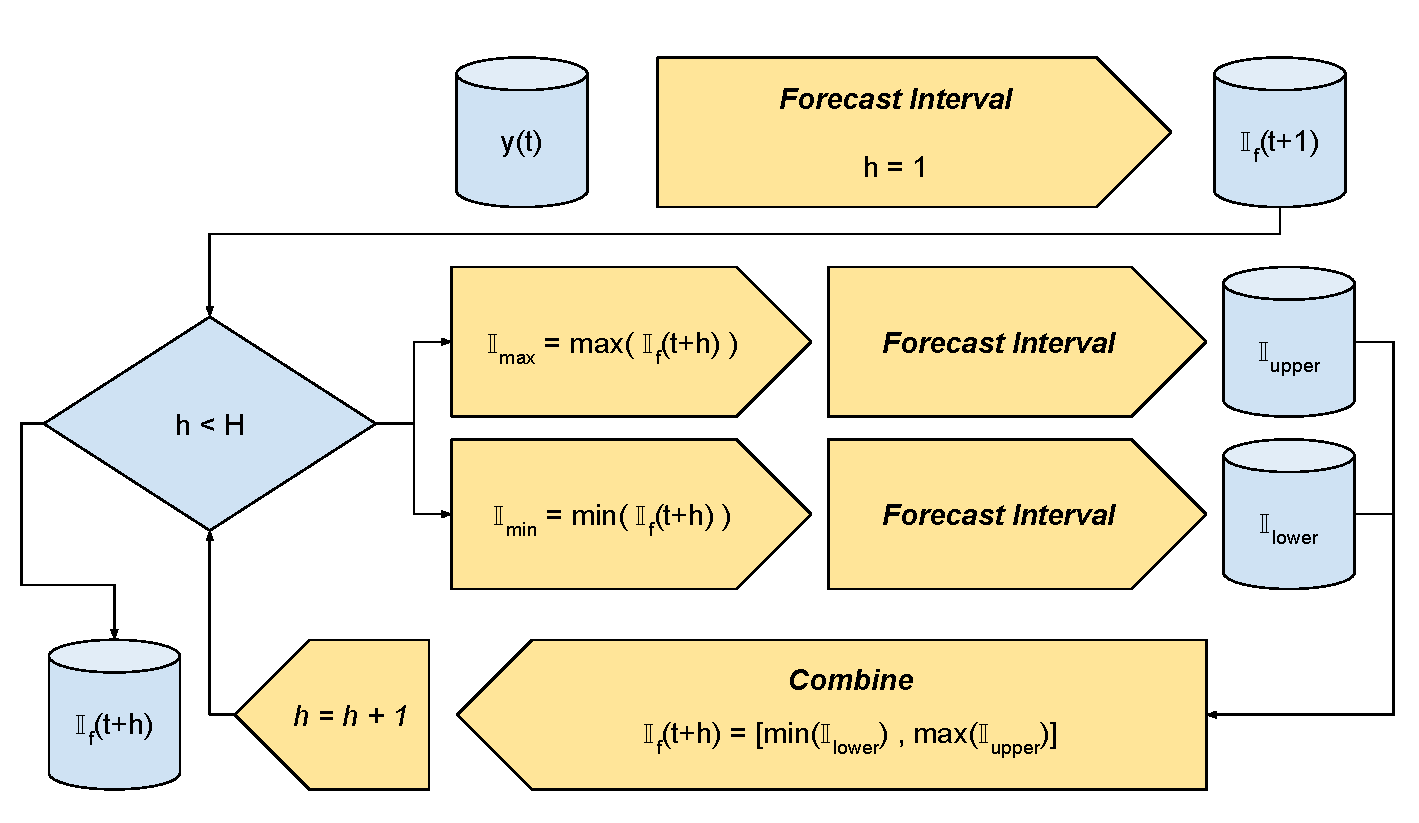
\includegraphics[width=\textwidth]{figures/ifts_many_steps.pdf}
    \caption{$\ifts$ many steps ahead interval forecasting procedure}
    \label{fig:ifts_many_steps}
\end{figure}

%%%%%%%%%%%%%%%%%%%%%%%%%%%%%%%%%%%%%%%%%%%%%%%%%%%%
%
%%%%%%%%%%%%%%%%%%%%%%%%%%%%%%%%%%%%%%%%%%%%%%%%%%%%
\subsection{Weighted $\ifts$}
\label{sec:wifts}

A weighted $\ifts$ extension use the same model building procedure  of WHOFTS method, presented in Section \ref{sec:fts_whofts} and aims to construct the weighted FLRG rule base $\model$. The prediction intervals are based on the weighted interval of the $RHS$ fuzzy sets on each FLRG weighted by their fuzzy membership in relation to input value.

$W\ifts$ extension also changes the Steps 3.a of the Forecasting Procedure, replacing the Equation \ref{eqn:iminimax} by the Equation \ref{eqn:weighted_iminimax}, where $\underline{\ufset}$ and $\overline{\ufset}$ represents respectively the lower and upper bounds of each fuzzy set $\ufset \in RHS$:

\begin{equation}
\begin{array}{ccc}
\intvl_{min} & = & \sum_{j \in RHS} w_j \cdot \underline{\ufset} \\
& & \\
\intvl_{max} & = & \sum_{j \in RHS} w_j \cdot \overline{\ufset}
\end{array}
\label{eqn:weighted_iminimax}
\end{equation}

\begin{figure}[htb]
    \centering
    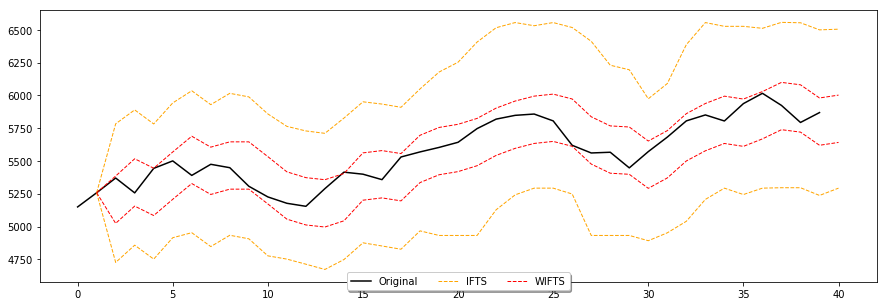
\includegraphics[width=\textwidth]{figures/ifts_sample_onestep.png}
    \caption{Sample of $\ifts$ and $W\ifts$ methods for one step ahead}
    \label{fig:ifts_sample_onestep}
\end{figure}

\begin{figure}[htb]
    \centering
    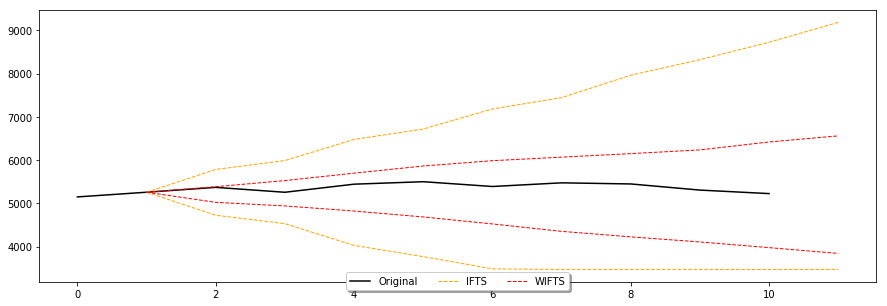
\includegraphics[width=\textwidth]{figures/ifts_sample_manystep.png}
    \caption{Sample of $\ifts$ and $W\ifts$ methods for many steps ahead}
    \label{fig:ifts_sample_manystep}
\end{figure}

Different from $\ifts$, which consider the extremum of the fuzzy sets, the generated interval $\intvl(t+1)$ of $W\ifts$ is bounded by a weighted composition of the fuzzy sets bounds, what make it more sharper. A sample of the method performance, for one and many steps ahead, can be seen in Figures \ref{fig:ifts_sample_onestep} and \ref{fig:ifts_sample_manystep}. 

Interval forecasts help to embrace the notion of forecast uncertainty, but did not offer a complete landscape of the uncertainty. In next sections, the probabilistic forecasting is presented as a more embracing way to represent the uncertainty.

%%%%%%%%%%%%%%%%%%%%%%%%%%%%%%%%%%%%%%%%%%%%%%%%%%%%
%
%%%%%%%%%%%%%%%%%%%%%%%%%%%%%%%%%%%%%%%%%%%%%%%%%%%%
\section{Probability Distribution Forecasts}\index{Probability Distribution Forecasts}
\label{sec:prob_distribution}

If the interval forecast represents a range of uncertainty, according to \cite{Krzysztofowicz2001} the probabilistic distribution forecast ``should quantify the total uncertainty that remains about the predictand, conditional on all information utilized on the forecasting process''. 

The probability distribution forecasts cover the complete range of the $U$ and can be continuous, using a probability density function, or discrete using both a discrete probability mass function or an empirical probability distribution, as histograms. In this last case, $U$ is split in $n$ equal length sub-intervals $b_i$ - called bins -, which are associated to a probability $p_i$ of occurrence, such as $\sum_{i=1}^n p_i = 1$. The length of each bin is the unit of discretization also referenced as the resolution of the distribution. 

Probability distribution forecasts can be represented also as the empirical cumulative probability distribution function $F(x) = n^{-1}\sum_{i\in Y(t)} \mathbf{1}(i < x)$ where $\mathbf{1}(c) = \{1$ if $c = True;\ 0,$ otherwise $\}$. Using $\alpha$-level prediction intervals, described on Section \ref{sec:prob_interval}, for $\alpha \in [0.05, ..., 0.5]$, is easy to construct the empirical distribution $F$ by iteration over the bounds of intervals. This approach was used to produce the distributions on Figure \ref{fig:arima}, from 7-steps ahead mean-variance prediction intervals over an ARIMA(2,0,0) model. The same approach can be used to construct probabilistic forecastings using QAR method, as shown in Figure \ref{fig:qar}.

The Gaussian Process Regression (GPR), as discussed in \cite{Rasmussen2006} and \cite{Roberts2013}, is a instance based parametric approach which interpolate the instances $y(t) \in Y$ and also produce an extrapolation for $y(t+1)$ in the form of a Gaussian Distribution. A Gaussian Process $\mathcal{GP}(m,\kappa)$ is defined by a mean function $m(Y)$ and covariance kernel $\kappa(y(i),y(j))$ which produce the covariance matrix $\Sigma$, such that $y(t+1) \sim \mathcal{N}(m(Y),\Sigma)$. The mean function $m(Y)$ is defined as the unconditional expectation of $Y$, such that $m(Y) = \mathbb{E}[Y]$. The covariance matrix $\Sigma$ assigns the similarity $\sigma_{ij} \in \Sigma$ between all pairs of instances of the time series, and it is defined by the covariance function $\sigma_{ij} = \kappa(y(i),y(j))$ for all $i,j = 1..T$. The covariance function is defined as $\kappa: U,U \rightarrow \mathbb{R}^+$ and measures the similarity between the two instances. 

The covariance function $\kappa$ is the most important parameter of $\mathcal{GP}$ model, and it is responsible to measure how the instances relate with themselves and with the time. $\kappa$ usually parameterized by a set of parameters or hyperparameters $\theta$, and because this $\kappa$ is also often written as $\kappa(y(i),y(j)|\theta)$ to make explicit the dependence on $\theta$. 

The most notable drawbacks of the GPR approach are the parametric assumption, the non-sparsity, i.e., it uses the whole set of samples to perform one prediction which is undesirable for Big Data scenarios, even with the fast and direct aproaches developed by \cite{Ambikasaran2014}, and it the fact the it loses efficiency as the number of variables grows.

\index{Bayesian Methods}\index{Bayesian Structural Time Series}\index{Space-State Models}

The Bayesian Structural Time Series (BSTS), discussed on \cite{Scott2014} and \cite{Barber2011a}, mix the well known State-Space models with the Bayesian Statistics approach for parameter estimation. A structural time series is a state-space model which associates the observed value $y(t)$ with an unobserved latent state  $\theta_t$. The structure is defined by a system of equations where the observation equation (also known as measurement equation) is defined in Equation \ref{eqn:observation} and the transition equation is defined in Equation \ref{eqn:transition}, an this system of equations can also be referred as a Linear Gaussian Model. 
\begin{align}
    y(t)  = & Z_ts_t + \epsilon_t & \epsilon_t \sim \mathcal{N}(0, H_t) \label{eqn:observation} \\
    s_t  = & T_t s_{t-1} + R_t\eta_t & \eta_t \sim \mathcal{N}(0, Q_t)  \label{eqn:transition}
\end{align}

An observed value value $y(t)$ is understood as a signal with noise, where the signal is the product of the unobserved state $s_t$ by the regressor parameter $Z_t$, and the noise (the extrinsic uncertainty) represented by the Gaussian error term $\epsilon_t$ whose variance is controlled by the parameter $H_t$. The unobserved latent state $s_t$ is represented by a vector with the several components of the time series, as trend, seasonality, level, etc, and is recursively defined by the transition matrix $T_t$ and the Gaussian error term $\eta_t$ (the intrinsic uncertainty), which in turn is controlled by the vector $R_t$ and the covariance matrix $Q_t$. The error terms $\epsilon_t$ and $\eta_t$ are mutually independent. This state-space representation can unify several approaches of time series forecasting and the parameters $Z_t,T_t,H_t,R_t$ and $Q_t$ defines the structure of the model, hereafter called as the $\Theta$ or the parameter space. For instance, for a ARMA approach the regressors are represented by $Z_t$ and the coefficients by $T_t$. 

Once the state space model is defined, it is necessary to infer the values of $Theta$ parameters from the training data $Y$, keeping in mind that $Y$ is a sample and it is composed with several sources of uncertainty, so it will be also $\Theta$. The Bayesian framework is employed in this task, which represent all uncertainties as probability distributions, from the learning process, passing through the parameter space $\Theta$, to the prediction space $U$. In such approach, the model parameters are probability distributions $P(\Theta|Y)$, reflecting the uncertainty around the real (but unknown) values of each parameter in $\theta \in \Theta$ given the learning sample $Y$. The forecast of $\estimate$ is a probability distribution $P(y(t+1)|\Theta,Y)$ that reflects the intrinsic uncertainty inherent of the time series $Y$, and the extrinsic uncertainty of the unknown real parameter values $P(\Theta|Y)$. 

The learning of the parameter space $\Theta$ is guided by the Bayes Rule. It states that, given a set of known evidences $d \in \mathcal{D}$ and a set of possible hypothesis $h \in \mathcal{H}$, the posterior distribution $P(h|\mathcal{D})$ is given by the Equation \ref{eqn:bayes}, where $P(\mathcal{H})$ is the prior distribution, the $P(\mathcal{D}|h)$ is the likelihood, and $P(\mathcal{D})$ is the normalizing term, such that $P(\mathcal{D}) = \sum_{h \in \mathcal{H}}P(\mathcal{D}|h)P(h)$ according to the Law of Total Probability. 

\begin{equation}
    P(h|\mathcal{D}) = \frac{P(\mathcal{D}|h) P(h)}{P(\mathcal{D})} = \frac{P(\mathcal{D}|h) P(h)}{\sum_{h \in \mathcal{H}}P(\mathcal{D}|h)P(h)}
    \label{eqn:bayes}
\end{equation}

The prior distribution $P(\mathcal{H})$ assigns the knowledge about the chances of each $h \in \mathcal{H}$ be the real value. The likelihood function $\mathcal{L}(h|\mathcal{D})$ assembles the plausibility of the evidences $d \in \mathcal{D}$ to have been generated by the parameter $h$, and it is equals to $P(\mathcal{D}|h)$.

Some methods are available to estimate the best hypothesis $h$ in the search space $\mathcal{H}$. The Maximum A Posteriori (MAP) principle poses the the best hypothesis $h \in \mathcal{H}$ is that one such that $h_{MAP} = argmax_\mathcal{H} P(h|\mathcal{D})$. Given that $P(\mathcal{D})$ is a constant and it is hard to compute, it is eliminated from the calculation, considering just $P(h|\mathcal{D}) \propto P(\mathcal{D}|h) P(h)$. The $h_{MAP}$ is used to update $P(\mathcal{H})$ and improve the aproximation of $P(\mathcal{H}|\mathcal{D})$ as new data is acquired. The Maximum Likelihood Estimation (MLE) method uses the average log-likelihood function $\hat{\mathcal{L}}(h|\mathcal{D}) =  |\mathcal{D}|^{-1}\sum_{i=0}^{|\mathcal{D}|} ln P(d_i|h)$ as a cost function, such that $h_{MLE} = argmax_\mathcal{H} \hat{\mathcal{L}}(h|\mathcal{D})$ is the best estimate parameter $h\in\mathcal{H}$. The drawback of these estimators is to estimate a unique point value without represent the uncertainty around the best hypothesis in $\mathcal{H}$.

However, the great strength of the Bayesian Methods is its ability to represent the uncertainties contained both on data and model parameters with probability distributions. In the other hand, this is also the great drawback of Bayesian Methods: their expensive computational cost. It is mainly because not all parts of its equation are always available - like the likelihood function $P(\mathcal{D}|h)$ - and those values need to be simulated using Monte Carlo methods.

\index{Monte Carlo Methods}

The Monte Carlo (MC) methods, initially proposed in \cite{Metropolis1949}, are techniques to solve complex  integration problems using random sampling. They aims to generate a set of samples $x_1,\ldots,x_n$ from a target distribution $\pi(x)$ in order to estimate some hard-to-compute feature $\phi(x)$ using the expected value $\mathbb{E}[\phi(x)] = n^{-1}\sum_i^n \phi(x_i)$ which converge to the unobserved real value of $\phi$. Given the estimated value as $\overline{\phi} = \mathbb{E}[\phi(x)]$, and its variance as $\phi_\sigma = Var[\phi(x)]$, some statistical concepts support the convergence of the MC methods. The Law of Large Numbers (LLN) asserts that, for a large enough number of samples $n$, the difference between the estimated value $\overline{\phi}$ and the true value $\phi$ decays to zero, or $P(\lim_{n\to\infty} |\overline{\phi} - \phi| = 0) = 1$ . The Central Limit Theorem (CLT) states that, for a large enough number of samples $n$, the $\overline{\phi}$ is normally distributed as $\overline{\phi} \sim \mathcal{N}(\phi,\phi_\sigma/n)$.

Markov Chain Monte Carlo (MCMC) methods improves the basic MC approach aiming to, instead of sample $\pi(x)$ directly, sample from a Markov Chain with a transition matrix $K$, where $K_{i,j} = P(x_t = i|x_{t-1} = j)$, such that the next sample $x_t$ be conditionally dependent of the previous $x_{t-1}$. The Markov Chain $K$ needs to approximate the real $\pi(x)$ distribution, but to estimate $K$ is very often an intractable problem. An approximation is provided by the Metropolis-Hastings algorithm generalized in \cite{Hastings1970}, which provide a simple and efficient way to simulate $K$ and generate samples. 

Estimate $P(\Theta|Y)$ using Bayesian methods is an optimization task which employ MCMC in order to sample from $P(Y|\Theta)P(\Theta)$ distribution while refine the parameters of $P(\Theta)$. The method demands the choosing of an appropriate a priori distribution $P(\Theta)$ that will rule the search space of each parameter $\theta \in \Theta$. The likelihood $P(Y|\Theta)$ estimate the fit of each parameter $\theta \in \Theta$ when generating samples of $y(t)\in Y$. This likelihood is itself another challenge once the samples $y(t)\in Y$ may be identically distributed but are not independent, there is a temporal dependence between $y(t)$ and it's past lags $y(t-1),...$ that must be respected. This problem demands the use of advanced MCMC methods as Sequential Monte Carlo, Sequential Importance Sampling and Particle Filters, deeply discussed in \cite{Smith2013}.

Once $\Theta$ values were estimated and represented by probability distributions $P(\Theta|Y)$, the estimation of $\estimate$ will be represented by a probability distribution $P(y(t+1)|\Theta,Y)$, defined on Equation \ref{eqn:posteriori}, which is also expensive to calculate and, again, needs to resort to MCMC methods. 

\begin{equation}
    P(y(t+1)|\Theta,Y) =  \int_U \int_\Theta P(y|\theta,Y)P(Y|\theta)P(\theta) dy d\theta
    \label{eqn:posteriori}
\end{equation}

A small sample of the BSTS method is shown in Figure \ref{fig:bsts}, for 7 steps ahead interval and probabilistic forecasting. If in one hand the Bayesian Structural Time Series are well succeeded in represent the intrinsic and extrinsic uncertainties, on the other hand it is complex to implement and computationally expensive to run, making it not applicable for a variety of scenarios where the time performance is mandatory.

\index{Forecast Combination}\index{Ensemble Forecasting}\index{Ensemble Learning}

There are other approaches to embody the  uncertainties of model parameters. Monte Carlo methods itself evoke the idea of forecast combination and Ensemble Methods, as posed in \cite{Smith2001}, ``In practice, ensemble forecasting is a Monte Carlo approach to estimating the probability density function (PDF) of future model states given uncertain initial conditions''. Forecast combination is not a new concept, see \citep{Clemen1989}, and start from the idea to mix different sources to improve forecasting. This is sightly close to the concept of Ensemble Methods defined by \cite{Gneiting2008} as ``an ensemble prediction system consists of multiple runs of numerical weather prediction models, which differ in the initial conditions''. Also \cite{Leutbecher2008} states that ``The ultimate goal of ensemble forecasting is to predict quantitatively the probability density of the state of the atmosphere at a future time''. 

Initially Ensemble Learning methods were developed to produce point forecasts as combination of the individual model's forecasts by a weighted average or more complex methods as Bayesian Model Averaging, for instance  \cite{Raftery2005}. Soon after, these methods were adapted for probabilistic forecasting as in \cite{Gneiting2005}, \cite{Leutbecher2008} and \cite{Fraley2013}. \cite{Xie2016} proposed a methodology for electric load probabilistic forecasting in three steps: \textit{pre-processing step} consisting of data cleaning;  \textit{forecasting step} using point-forecasting methods, forecast combination and scenario-based probabilistic forecasting; \textit{post-processing step} performing a simulation on the residuals of the selected point forecasting models in order to improve the probabilistic forecast.

These ensembles can be homogeneous (same method with different parameters) or hybrid (different methods with different parameters). This set of models $\mathcal{M}$ receive a set of parameters $\Theta$ to produce a set of forecasts $\estimate$, such as $\estimate^i = m_i(\theta_i)$, $\forall m_i \in \mathcal{M}$ and the $\theta_i\in \Theta$ values are drawn of a prior probability distribution $P(\Theta)$. The methods can be executed several times and as large the sample is, best approximations are made. After $n$ runs, the empirical distribution $P(y(t+1))$ of the outputs is available.

Ensemble Learning is an extent of the Ensemble Forecasting on Machine Learning field, defined by \cite{Brown2010} as ``the procedures employed to train multiple learning machines and combine their outputs with individual predictions combined appropriately, should have better overall accuracy, on average, than any individual committee member''. Ensemble Learning can be used in classification in regression tasks, also time series forecasting as in \cite{Chen2005}, \cite{Bai2010} and \cite{Koskova2015a}.

This concept is exploited in \cite{Mohammed2015} and \cite{Mohammed2016},  which proposed an ensemble learning approach for solar power probabilistic forecasting based on k-Nearest Neighbors, Regression Trees, Random Forests and regression methods. Given an ensemble with $k$ models and taken the ordered set of the $k$ individual forecasts, the probabilistic forecast is constructed as an empirical cumulative distribution $F$, calculated with the percentiles of the individual forecasted values. $F$ can be made with three approaches: \textit{quantile linear interpolation}, \textit{normal distribution} and \textit{normal distribution with initial different conditions}. The linear interpolation approach calculate the $\tau$ quantile position $r_\tau$ on the individual forecasts as $r_\tau = \frac{k\tau}{100}+0.5$. The normal distribution approach is similar to mean-variance model of section \ref{sec:prob_interval}. With the set of individual forecasts is calculated the mean $\mu$ and variance $\sigma$ and the $\tau$ quantile is given by $\tau = \mu + z_\tau\cdot\sigma$. The third approach is specific for the application domain of solar power.

The advantage of \cite{Mohammed2015} approach is the flexibility and ease of implementation, since the individual models can be replaced (or added) for any other point forecaster, for instance, any FTS method. As more models are added to the ensemble, better will be the probabilistic distributions but also become more computationally expensive. 

\index{Kernel Density Estimation}\index{Kernel Dressing}

Other distributions generating techniques for ensemble forecasts exist as Kernel Density Estimation \citep{Hong2016a} and Kernel Dressing [ \citep{Pinson2009} and \citep{Brocker2008}] and can be easily combined with instance-based methods as k-nearest neighbors. Both approaches smooth the discrete values in a continuous function that approximate the empirical distribution of data, as exposed in Equation \ref{eqn:kde}, where $Y$ is the set of individual forecasts, $K$ is the kernel function and $h$ is a smoothing parameter also known as bandwidth.:

\begin{equation}
P(x) = (nh)^{-1} \sum_{i \in Y} K\left(\frac{x - i}{h}\right)
\label{eqn:kde}
\end{equation}

A kernel function $K$ have to be a non-negative, real-valued, symmetric, integrable and normalized, such that $\int_{-\infty}^{+\infty}K(u) du = 1$. A review of density estimation methods can be found in \cite{Silverman1986} and a specific study on estimation of $h$ parameter can be found in \cite{Sheather1991}. A small sample of the kNN with KDE approach is shown in Figure \ref{fig:knn}, for 7 steps ahead interval and probabilistic forecasting. 

\begin{table}[]
    \centering
    \begin{tabular}{|c|c|} \hline
        \textbf{Kernel} & \textbf{Definition} \\ \hline
        Triangular & $K(u) = 1 - |u|$ \\ \hline
        Tophat & $K(u) = \frac{1}{2}\mathbb{I}(|u| < 1)$ \\ \hline
        Epanechnikov & $K(u) = 3/4(1-u^2)$ \\ \hline
        Gaussian & $K(u) = \frac{1}{\sqrt{2\pi}}e^{-1/2u^2}$ \\  \hline
    \end{tabular}
    \caption{KDE Kernels}
    \label{tab:kde_kernels}
\end{table}

The several methods pointed in this section are spread in literature. In the next section accuracy measures for probabilistic forecasting are discussed.

%%%%%%%%%%%%%%%%%%%%%%%%%%%%%%%%%%%%%%%%%%%%%%%%%%%%
%
%%%%%%%%%%%%%%%%%%%%%%%%%%%%%%%%%%%%%%%%%%%%%%%%%%%%
\subsection{Accuracy Measures for Probabilistic Forecasts}
\label{sec:prob_probabilistic_measure}
\index{Accuracy Measures}\index{Probabilistic Forecast Accuracy Measures}
\index{Accuracy Measures for Probabilistic Forecasts}

As the probabilistic forecast provides the landscape of uncertainty for the whole $U$, it is also possible to use the accuracy measures presented on Sections \ref{sec:prob_point_measures} and \ref{sec:prob_interval_measures} to asses its accuracy. A probability distribution can be reduced to a point using its expected value $\mathbb{E}$ or it's median $m = F(.5)$. In both cases, the point forecasting accuracy values can be used to asses its accuracy.

A probability distribution $P$ can also be expressed in terms of intervals as well, by using $\alpha$-levels and their respective quantiles. In this case, the prediction interval accuracy measures can be used to evaluate $P$ accuracy in several different $\alpha$, in the many different aspects discussed in section \ref{sec:prob_interval_measures}.

But pure probabilistic accuracy measures want to asses how well the probabilities of $P$ are spread over $U$ when we know the true value $y(t)$, and how close $P$ were able to predict the uncertainty around $y(t)$. The most simple probabilistic forecasting measure is the Logarithm Score (LS), proposed in \cite{Good1952} and defined in \ref{eqn:log_score}, which indicates how strong was the probability distribution $P$ to predict the real value $y(t)$. The Logarithm Score presents some limitations as, for instance, when $P(y(t)) = 0$ then $LS(P,y(t)) = \infty$.

\begin{equation}
    LS(P,Y) = T^{-1} \sum_{t=1}^T -log(P(y(t)))
    \label{eqn:log_score}
\end{equation}

\index{Brier Score}

The Brier Score (BS), proposed in \cite{Brier1950} and defined in Equation \ref{eqn:brier_score}, was originally defined for $R$ categorical events but it is possible to extend it for numeric values by splitting the Universe of Discourse in $R$ bins, or to consider the quantiles. This score can be interpreted as the Mean Squared Error (MSE) from the predicted probabilities for each bin $r$, represented by $P(r)$, to the real observed events represented by $\mathbf{1}\{ y(t) \in r\}$.

\begin{equation}
    BS(P,Y) = T^{-1} \sum_{t=1}^T \sum_{r=1}^R ( P(r) - \mathbf{1}\{ y(t) \in r\})^2
    \label{eqn:brier_score}
\end{equation}

\index{Continuous Ranked Probability Score}\index{CRPS}\index{Probabilistic forecast metrics}

The metric chosen to assess the distributions is the Continuous Ranked Probability Score (CRPS). CRPS is a proper measure for probabilistic forecasts, defined by  \cite{Gneiting2007b} as Equation \eqref{eqn:crps1} for one forecast and by \cite{Gneiting2007b} as Equation \eqref{eqn:crps2} for more than one forecasts. CRPS provides a direct way to benchmark probabilistic forecast since it is expressed in the same unit as the observed variable and is a generalization of the Mean Absolute Error (MAE). Therefore, the perfect score for CRPS, as in MAE, is 0.

\begin{equation}
CRPS(F,) = \int_{-\infty}^{+\infty} (F(y) - \mathbf{1}\{y \geq x\})^2  dy
\label{eqn:crps1}
\end{equation}

\begin{equation}
CRPS(F) = \frac{1}{N} \sum_{1}^{N} \int_{x=-\infty}^{x=+\infty} (F(y) - \mathbf{1}\{y \geq x\})^2  dy
\label{eqn:crps2}
\end{equation}
where $F$ is the cumulative distribution function (CDF) of the forecasted distribution, $x$ is  an, $\mathbf{1}\{y \geq x\}$ is the Heavyside function representing the CDF of this punctual value.

%%%%%%%%%%%%%%%%%%%%%%%%%%%%%%%%%%%%%%%%%%%%%%%%%%%%
%
%%%%%%%%%%%%%%%%%%%%%%%%%%%%%%%%%%%%%%%%%%%%%%%%%%%%
\subsection{Fuzzy Time Series Methods With Probabilistic Background}
\index{Fuzzy Probabilistic Models}

The first studies to make the relationship of probabilities with fuzzy sets came from Prof. Zadeh, \cite{Zadeh1968}, \cite{Zadeh1984}, which defines the fuzzy set probability as the expectation of the membership function. Also, Klement, Schwyhla and Lowen \cite{ErichPeterKLEMENT1981} and \cite{Dubois1989} explore the relationships between the fuzzy membership functions and the probability measures based on Measure Theory. 

These theoretical works form the base of the Fuzzy Stochastic Fuzzy Time Series (FSFTS) of Song, Leland and Chissom \cite{Song1997}, where three models were presented but there is no empirical analysis of their results. In this work the probability space $[0,1]$ is also described by a linguistic variable $\tilde{P}$ with few fuzzy sets that describe the probability in linguistic terms like "low","medium","high". The rules of the model are composed by tuples $(p_j,\ufset)$ where $p_j \in \tilde{P}$ and $\ufset \in \ulvar$ and the deffuzyfication weight the fuzzy sets by their fuzzy probability.

 \cite{Gangwar2014} proposed the \textit{Probabilistic and Intuitionistic Fuzzy Time Series} - PIFTS method, strongly based on data normality and explicit Gaussian Process assumption. \cite{Cheng2012} and \cite{Chuang2014} use the Song and Chissom relation matrix and a Hidden Markov Chains for generating simulations for forecasting step, the \textit{Probabilistic Smoothing Hidden Markov Model FTS} - psHMM-FTS, which has high computational cost.

%%%%%%%%%%%%%%%%%%%%%%%%%%%%%%%%%%%%%%%%%%%%%%%%%%%%
%
%%%%%%%%%%%%%%%%%%%%%%%%%%%%%%%%%%%%%%%%%%%%%%%%%%%%
\section{The Ensemble FTS Method}
\label{sec:ensemblefts}\index{EnsembleFTS}

The $\ifts$ represented the forecasting uncertainty using the mean of the bounds of the fuzzy sets, or the empirical uncertainty, without probabilistic sense. However, the FTS methods use of several ways to represent the time series uncertainties, as the number of partitions $k$, order $\Omega$, lag indexes $L$, rule weights. There are uncertainties surrounding these values due the ontological uncertainty of the data, uncertainties that will be reduced - but not removed - after the optimization of the hyper-parameters proposed on Chapter \ref{chap}.

A way to encompass these uncertainties is to generate a meta model $\model$, composed with several FTS models $m \in \model$, such that each one of these individual models is trained with different values of FTS hyper-parameters, which aims to represent the hyper-parameter uncertainty and its effects. The aggregation of the individual forecasts $\estimate_m$ produced by each $m \in \model$ can represent the overall probabilistic uncertainty $P$ over the possible values of $y(t+1) \in U$ using kernel density estimation seen in Section \ref{sec:prob_distribution}.

Several approaches can be adopted to represent the uncertainty of the hyper-parameter, from varying the number of partitions and order, passing through varying the partitioning methods, until varying the FTS method itself. However, the present approach adopt a conventional rule-based high order FTS method with a Grid partitioning method, varying only the number of partitions $k$ and order $\Omega$.

On EnsembleFTS the hyper-parameters $k$ and $\Omega$ are intervals and not scalar values. During the training procedure, explained in Section \ref{sec:ensemblefts_training} a FTS model will be trained for each combination of individual values in the Cartesian Product of $k$ and $\Omega$. On the forecasting procedure detailed in Section \ref{sec:ensemblefts_forecasting}, the input sample is presented for all internal models e their outputs are aggregated using a KDE, producing a probability distribution $P:U \rightarrow [0,1]$. Besides $k$ and $\Omega$ ranges, the kernel function $K$ and its bandwidth parameter $h$ are also parameters of the model.

%%%%%%%%%%%%%%%%%%%%%%%%%%%%%%%%%%%%%%%%%%%%%%%%%%%%
%
%%%%%%%%%%%%%%%%%%%%%%%%%%%%%%%%%%%%%%%%%%%%%%%%%%%%
\subsection{Training Procedure}
\label{sec:ensemblefts_training}\index{Ensemble FTS Training Procedure}\index{Training Procedure}

The aim of the training procedure is to build an ensemble $\model$ with $k\times\Omega$ individual models $m_i$, given a crisp training set $Y$. The overall training procedure is shown in Figure \ref{fig:ensemblefts_training} and it is composed as follows:

\begin{figure}[htb]
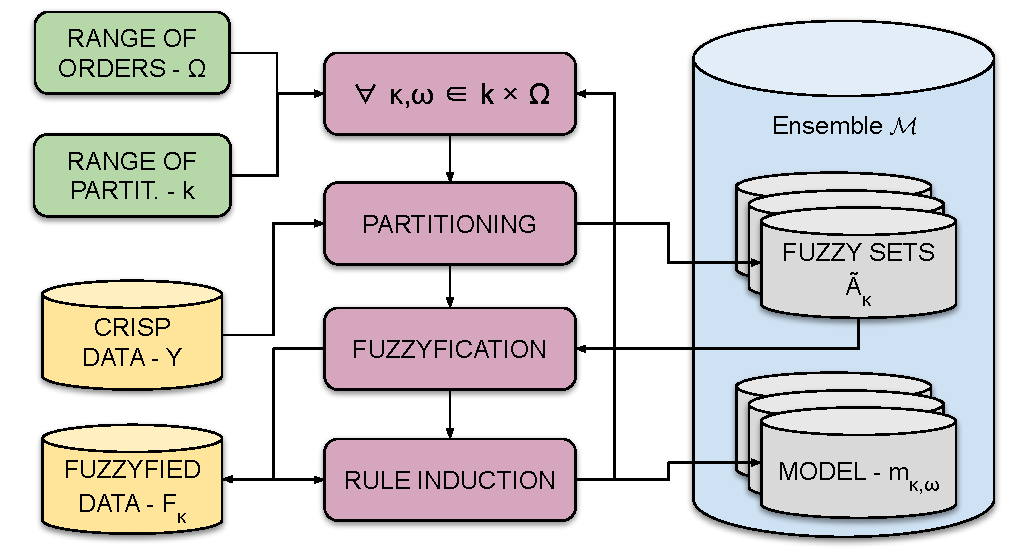
\includegraphics[width=\textwidth]{figures/ensemblefts_training.pdf}
\caption{Ensemble FTS training procedure}
\label{fig:ensemblefts_training}
\end{figure}

\begin{enumerate}
\item[Step 1] \textit{Main Loop}: For each pair $(\kappa,\omega)$ created by the cartesian product of each $\kappa \in k$ with each $\omega \in \Omega$, repeat the Steps 2 to 5;
\item[Step 2] \textit{Partitioning}: Create a linguistic variable $\ulvar_\kappa$ over $U$ with $\kappa$ fuzzy sets using the Grid partitioning method and triangular $\mu$;
\item[Step 3] \textit{Fuzzyfication}: Fuzzyfy the crisp time series $Y$ using the linguistic variable $\ulvar_\kappa$, creating the fuzzyfied time series data $F_\kappa$;
\item[Step 4] \textit{$\omega$-order model}: With $F_\kappa$, use the high order weighted rule knowledge model to infer  $\omega$-order fuzzy rules and compose the model $m_{\kappa,\omega}$;
\item[Step 5)] \textit{Ensemble}: Append the model $m_{\kappa,\omega}$ on $\model$;
\end{enumerate}

%%%%%%%%%%%%%%%%%%%%%%%%%%%%%%%%%%%%%%%%%%%%%%%%%%%%
%
%%%%%%%%%%%%%%%%%%%%%%%%%%%%%%%%%%%%%%%%%%%%%%%%%%%%
\subsection{Forecasting Procedure}

With the ensemble $\model$ built as in previous section, and given an input test sample $y(t)$, it is desired to forecast a full probability distribution $P(y(t+1)|y(t))$. The overall process is described in Figure \ref{fig:ensemblefts_forecasting} and is composed by: a) the forecasting of individual models; b) forecast selection and c) distribution smoothing with the KDE. The complete procedure is detailed below:

\begin{figure}[htb]
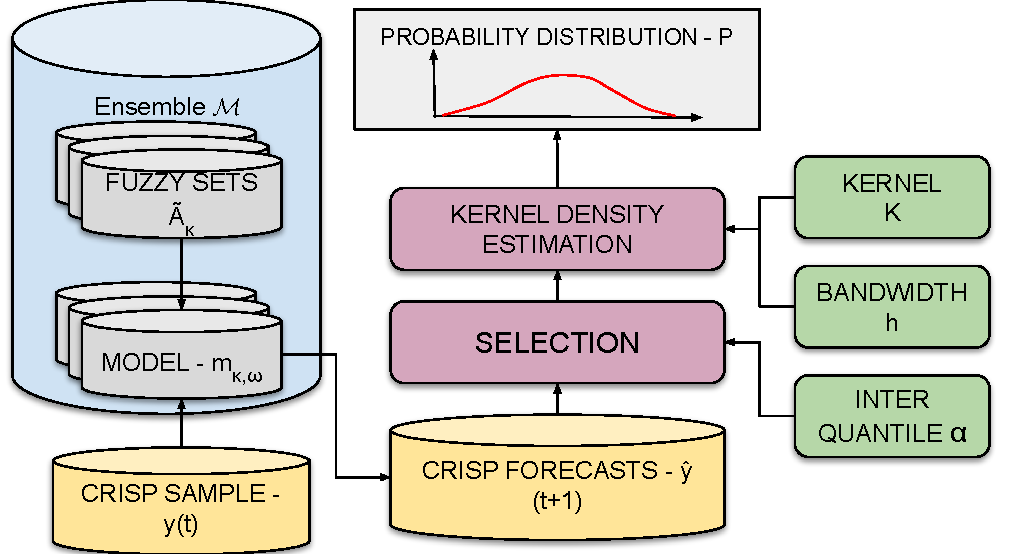
\includegraphics[width=\textwidth]{figures/ensemblefts_forecasting.pdf}
\caption{Ensemble FTS forecasting procedure}
\label{fig:ensemblefts_forecasting}
\end{figure}

%%%%%%%%%%%%%%%%%%%%%%%%%%%%%%%%%%%%%%%%%%%%%%%
\begin{enumerate}

\item[Step 1] \textit{Individual forecasts}: The input sample $y \in Y$ is presented to each internal model each model $m_j \in \model$, which in turn will produce a individual forecast $\hat{y}_j(t+1)$. The set of crisp forecasts is hereafter called $\hat{y}(t+1)$.

%%%%%%%%%%%%%%%%%%%%%%%%%%%%%%%%%%%%%%%%%%%%%%%
\item[Step 2] \textit{Forecast selection}: In order to control the total forecast variance and eliminate the effect of possible outliers the forecasted output is limited by an inter quantile interval $(\alpha, 1-\alpha)$ where $\alpha \in (0,1)$ is the confidence level. By varying $\alpha$ parameter it is possible to fine tune the final distribution accuracy by eliminating forecasts that are too distant from the mean.

%%%%%%%%%%%%%%%%%%%%%%%%%%%%%%%%%%%%%%%%%%%%%%%
\item[Step 3] \textit{Kernel density estimation}: The set of crisp forecasts $\hat{y}(t+1)$ is used with a kernel density estimator $K$ to estimate the probability distribution $P_{t+1}: U \rightarrow [0,1]$. Two parameters are necessary on this step: the type of kernel and the bandwidth $h$. Both parameters are domain specific and need to be empirically evaluated for each application.

\item[Step 4] \textit{Many steps ahead forecast}:If the forecasting horizon is $H > 1$, define $P_H = \{P_{t+1}\}$ as the set of intervals and repeat the below steps for each $h=2..H$, otherwise return  $P_{t+1}$.
\begin{enumerate}
    \item[a)]  Find the quantiles $Q = \{.1, .2, .3., .4, .5, .6, .7, .8, .9\}$ of the the last $max(\Omega)$ forecasted sets $\hat{y}(t-\omega)$, $\forall \omega \in \Omega$, such that $\hat{y}_Q(t-\omega) = \{ Q_\tau(\hat{y}(t-\omega) | \tau \in Q)$ where $Q$ is the Quantile Function;
    \item[b)] Apply a Cartesian Product between the quantiles of the last $max(\Omega)$ forecasted sets, such that $\hat{Y} = \prod_{\omega \in \Omega} \hat{y}_Q(t-\omega)$; 
    \item[c)] Use each sample $\hat{y}(t) \in \hat{Y}$ as input to Step 1 and 2 and aggregate all the results on the set $\hat{y}(t+1)$
    \item[d)] Use $\hat{y}(t+1)$ with Step 3 to produce $P_{t+h}$ and include it on $P_H$. If $h=H$ then return $P_H$.
\end{enumerate}

\end{enumerate}

The probabilistic forecast $P(y(t+1)|y(t))$ aims to represent $\estimate \in U$ uncertainties of the model $\model$ in relation to $k$ and $\Omega$. A sample of the EnsembleFTS for one step and many steps ahead forecasts can be seen in Figures \ref{fig:ensemblefts_sample_onestep} and \ref{fig:ensemblefts_sample_manystep}. 

\begin{figure}[htb]
    \centering
    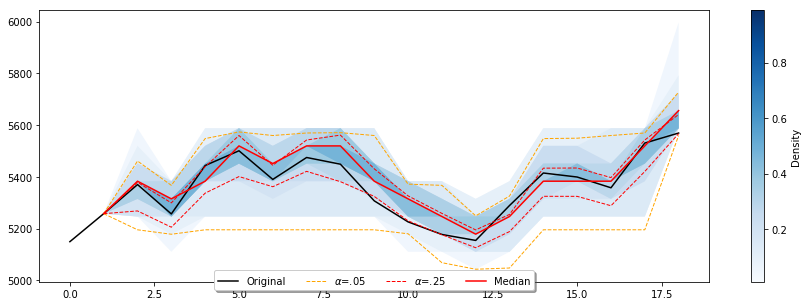
\includegraphics[width=\textwidth]{figures/ensemblefts_sample_onestep.png}
    \caption{Sample of EnsembleFTS performance for one step ahead}
    \label{fig:ensemblefts_sample_onestep}
\end{figure}

\begin{figure}[htb]
    \centering
    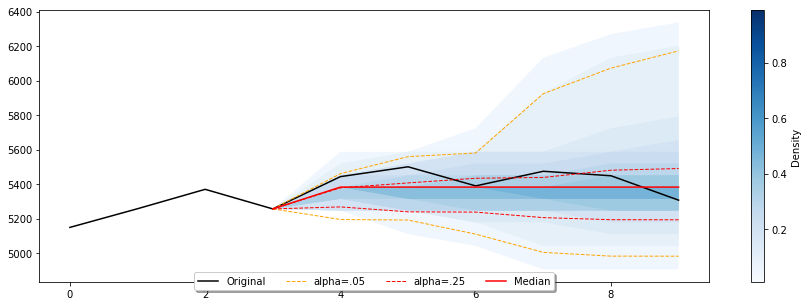
\includegraphics[width=\textwidth]{figures/ensemblefts_sample_manystep.png}
    \caption{Sample of EnsembleFTS performance for many steps ahead}
    \label{fig:ensemblefts_sample_manystep}
\end{figure}

%%%%%%%%%%%%%%%%%%%%%%%%%%%%%%%%%%%%%%%%%%%%%%%%%%%%
%
%%%%%%%%%%%%%%%%%%%%%%%%%%%%%%%%%%%%%%%%%%%%%%%%%%%%
\section{Computational Experiments}
\label{sec:prob_experiments}

In this section presents an empirical study of the performance of the proposed methods  using three economic time series. Initially, the datasets, design of experiments and statistical tests employed are discussed. In Section \ref{sec:prob_hyperparameters}, the accuracy sensitivity regarding to the hyperparameters of the proposed methods are analyzed using a grid search. In Section \ref{sec:prob_experiments_interval} the results of the interval forecasting  experiments are presented and discussed and then, on Section \ref{sec:prob_experiments_probabilistic}, the probabilistic forecasting experiments are analyzed.

To measure the performance of the proposed models were chosen ARIMA, QAR, kNN/KDE and, BSTS as competitor models due its possibility to perform interval and probabilistic forecasting for many steps ahead. The hyperparameters of each method were individually investigated and only the best model is taken account on the validation of the results.

For these experiments three well known financial time series data (the TAIEX, S\&P 500 and NASDAQ data sets) were selected each of them with 5000 instances, whose descriptions and properties can be found at Appendix \ref{apd:monovariate_datasets}. A rolling window cross-validation methodology \cite{Tashman2000} was applied, using a working set of 1000 instances, 800 for training (80\%) and 200 for testing (20\%) and a sliding increment of 200 instances, totaling 23 experiments, and all measurements were performed out of sample.

Once the model fine tune was performed for each method and the experiments were executed for each dataset, statistical tests were employed in order to compare the performance of the models. The hypothesis testing procedures adopted best practices discussed in \cite{Garcia2010,Derrac2011,Trawinski2012}. The Friedman Aligned Ranks test \cite{friedmanalignedrankstest} non parametric procedure was adopted to test the equality of the means, where the null hypothesis $H_0$ stands for the equality of all means and the inability to distinguish between the methods and the alternative hypothesis $H_1$ stands for the difference of the means and the distinguishability between the models. The paired \textit{post hoc} procedure adopted was the Finner test \cite{finnertest}, in a one-versus-all design where the PWFTS method is taken as a control method. In Finner test  the null hypothesis $H_0$ stands for the equality between the control and the test methods and the alternative hypothesis $H_1$ stands for the significant difference between the control and test methods. All the tests adopted the significance level $\alpha = .05$ and were performed on STAC framework \cite{stac}, and all FTS methods were tested with the pyFTS library\footnote{\url{https://pyfts.github.io/pyFTS/}. Access in 01/07/2018} \cite{pyFTS}. 

In order to contribute to the replication of all the results in the research, all data and source codes employed in this chapter are available at the URL:
\texttt{\url{http://bit.ly/scalable_probabilistic_fts_chap3}}

%%%%%%%%%%%%%%%%%%%%%%%%%%%%%%%%%%%%%%%%%%%%%%%%%%%%
%
%%%%%%%%%%%%%%%%%%%%%%%%%%%%%%%%%%%%%%%%%%%%%%%%%%%%
\subsection{Hyperparameter Grid Search}
\label{sec:prob_hyperparameters}

In order to asses the impact of the $\ifts$ and W$\ifts$ methods hyperparameters on the accuracy, a Search Grid was performed for each benchmark dataset, using the search spaces contained on Table \ref{tab:ifts_gridsearch}. The Winkler Score accuracy metric, where  $\alpha \in \{.05,.25\}$, for each method, order, dataset and partitions can be observed on Figures \ref{fig:ifts_gridsearch} and \ref{fig:wifts_gridsearch}. It is notable that $\ifts$ has more sensitivity to the number of partitions than W$\ifts$. This occurs because the length of the partitions is the mechanism used by $\ifts$ method to adjust the importance of each fuzzy set. W$\ifts$ in the other hand use the rule weights to balance the importance of each fuzzy set on deffuzyfication, diminishing the impact of the partition length.   

Once several numbers of partitions and order values achieved very closed accuracy values, the Principle of Parsimony (or Occam's Razor) was adopted to chose the set of hyperparameters that leads to smallest number of rules $|\model|$, keeping the same accuracy. The chosen hyperparameters were $k = 45$ and $\Omega = 1$ and a sample of the best models performance can be seen in Figures \ref{fig:ifts_sample_onestep} and \ref{fig:ifts_sample_manystep}.

\begin{table}[htb]
    \centering
    \begin{tabular}{|c|c|c|c|} \hline
        Hyperparameter & Search space  \\ \hline
        $k$ & $\{10, 15, 20, 25, 30, 35, 40, 45, 50\}$  \\ \hline
        $\Omega$ & $\{1, 2, 3\}$ \\ \hline
    \end{tabular}
    \caption{Hyperparameter search spaces for IFTS and WIFTS grid search}
    \label{tab:ifts_gridsearch}
\end{table}

\begin{figure}[htb]
    \centering
    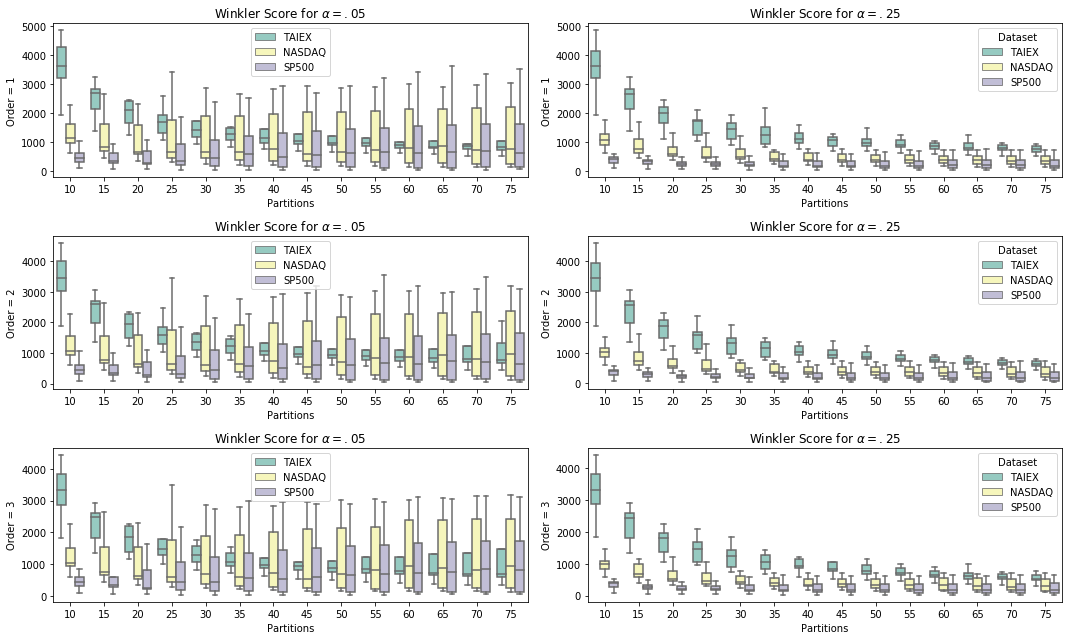
\includegraphics[width=\textwidth,height=15cm]{figures/ifts_gridsearch.png}
    \caption{IFTS Winkler Scores for $\alpha \in \{.05, .25\}$ by dataset, order and partitions}
    \label{fig:ifts_gridsearch}
\end{figure}

\begin{figure}[htb]
    \centering
    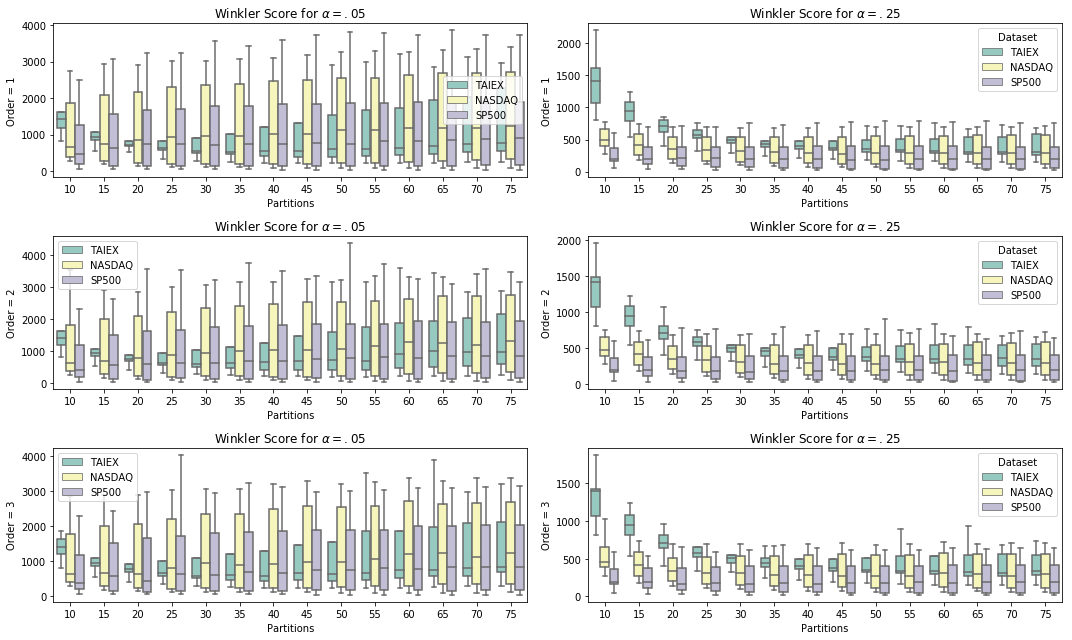
\includegraphics[width=\textwidth,height=15cm]{figures/wifts_gridsearch.png}
    \caption{WIFTS Winkler Scores for $\alpha \in \{.05, .25\}$ by dataset, order and partitions}
    \label{fig:wifts_gridsearch}
\end{figure}



The EnsembleFTS method has a different hyperparameter set than $\ifts$ and W$\ifts$ methods. As a meta-model, an internal FTS model should be chosen, beyond the $k$ range and the $\Omega$ range. To reduce the complexity of this search space a set of four models were predefined and detailed in Table \ref{tab:ensemblefts_gridsearch}. The accuracy of EnsembleFTS was analyzed using both interval and probabilistic perspectives, the first one using the Winkler Score interval accuracy metric, for  $\alpha \in \{.05, .25\}$, and second one using CRPS probabilistic metric. The Winkler Score for each method and dataset is shown in Figures \ref{fig:ensemblefts_winklerscore}, where can be observed that the Model 4 is most stable model. The CRPS results are shown in Figure  \ref{fig:ensemblefts_crps}, where  can be observed that Model 4 again is the more stable model. The immediate conclusion is that the higher diversity of models help KDE to build a more precise probability distribution, with improved sharpness and resolution.  A sample of the Model 4 performance can be seen in Figures \ref{fig:ensemblefts_sample_onestep} and \ref{fig:ensemblefts_sample_manystep}, with $\alpha \in \{.05, .25\}$ prediction intervals and probabilistic forecasting for 7 steps ahead.  

\begin{table}[htb]
    \centering
    \begin{tabular}{|c|c|c|c|} \hline
        Name & Internal Model & $k$ range & $\Omega$ range  \\ \hline
        Model 1 & HOFTS & $\{10, 20, 30, 40, 50\}$ & $\{1, 2, 3\}$ \\ \hline
        Model 2 & HOFTS & $\{10, 15, 20, 25, 30, 35, 40, 45, 50\}$ & $\{1, 2, 3\}$ \\ \hline
        Model 3 & WHOFTS & $\{10, 20, 30, 40, 50\}$ & $\{1, 2, 3\}$ \\ \hline
        Model 4 & WHOFTS & $\{10, 15, 20, 25, 30, 35, 40, 45, 50\}$ & $\{1, 2, 3\}$ \\ \hline
    \end{tabular}
    \caption{Search spaces for Ensemble FTS grid search}
    \label{tab:ensemblefts_gridsearch}
\end{table}

\begin{figure}[htb]
    \centering
    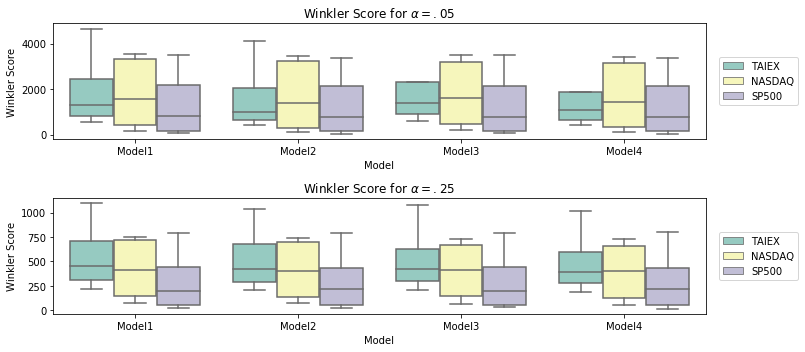
\includegraphics[width=\textwidth]{figures/ensemblefts_winklerscore.png}
    \caption{Sample of IFTS and WIFTS for 7 steps ahead}
    \label{fig:ensemblefts_winklerscore}
\end{figure}

\begin{figure}[htb]
    \centering
    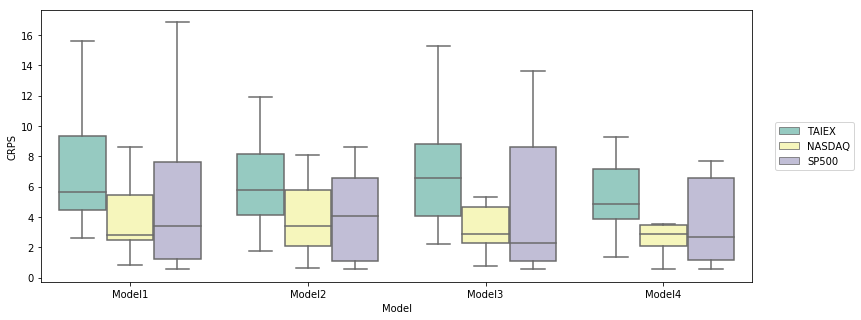
\includegraphics[width=\textwidth]{figures/ensemblefts_crps.png}
    \caption{CRPS response of EnsembleFTS}
    \label{fig:ensemblefts_crps}
\end{figure}

%%%%%%%%%%%%%%%%%%%%%%%%%%%%%%%%%%%%%%%%%%%%%%%%%%%%
%
%%%%%%%%%%%%%%%%%%%%%%%%%%%%%%%%%%%%%%%%%%%%%%%%%%%%
\subsection{Interval Forecasting Benchmarks}
\label{sec:prob_experiments_interval}

The Winkler Score Mean results for each method and dataset are presented in Table \ref{tab:prob_interval_results}. The Friedman Aligned Ranks of the methods are presented on Table \ref{tab:prob_interval_ranks} and the test statistic for these results is $Q = 12.891861761426975$, where the p-Value is $P(\chi^2_{df} < Q) = 0.04478569463323567$, with $df=5$ degrees of freedom. For this statistic the $H_0$ is rejected at the $\alpha=.05$ confidence level, indicating that there is difference between the means of the competitor models.

The \textit{post-hoc} tests were employed using $\ifts$, $W\ifts$ and EnsembleFTS methods as control methods and their results are presented on Tables \ref{tab:prob_interval_posthoc_ifts}, \ref{tab:prob_interval_posthoc_wifts} and \ref{tab:prob_interval_posthoc_ensemblefts}, showing there is no prevalence of the methods except of $W\ifts$ over BSTS. These results showed that $\ifts$, $W\ifts$ and EnsembleFTS interval forecasting methods perform satisfactorily when compared with the standard methods in literature. 

The statistical tests were employed on the one step ahead forecasts. The Figure \ref{fig:interval_many_steps} shows, for each method and dataset, the impact of the forecasting horizon on the Winkler Score accuracy.

\begin{table}[h]
\resizebox{\textwidth}{!}{% <------ Don't forget this %
\centering
    \begin{tabular}{|c|ccccccc|}
\hline
\textbf{Dataset } & \textbf{ ARIMA } & \textbf{ QAR } & \textbf{ WIFTS } & \textbf{ IFTS } & \textbf{ kNN } & \textbf{ EnsembleFTS } & \textbf{ BSTS} \\
\hline
\multirow{2}{*}{S\&P 500} &      72.712 &    121.694 &    111.705 &    113.516 &    131.394 &     268.567 &     292.415 \\
&   $\pm$  135.871 &  $\pm$  319.305 &  $\pm$  156.013 &   $\pm$  91.627 &   $\pm$  166.31 &   $\pm$  318.259 &   $\pm$  384.499 \\ \hline
\multirow{2}{*}{NASDAQ} &     233.261 &    106.416 &     123.35 &    284.692 &    170.709 &     603.881 &     652.036 \\
&   $\pm$  486.735 &   $\pm$  56.248 &  $\pm$  141.251 &   $\pm$  147.24 &  $\pm$  156.097 &   $\pm$  638.297 &   $\pm$  963.624 \\ \hline
\multirow{2}{*}{TAIEX} &     858.124 &        340 &    480.581 &    917.879 &    428.484 &     898.531 &     1280.67 \\
&  $\pm$  1337.139 &   $\pm$  269.34 &  $\pm$  561.826 &  $\pm$  243.737 &  $\pm$  269.459 &  $\pm$  1175.107 &  $\pm$  1472.031 \\ \hline
\end{tabular}
}
    \caption{Average Winkler Score with $\alpha=.05$ for one step ahead interval forecasts}
    \label{tab:prob_interval_results}
\end{table}

\begin{table}[hbt]
    \centering
    \begin{tabular}{|c|c|}
\hline
       METHOD &       RANK \\
\hline
          QAR &   5.333333 \\
        WIFTS &   5.666667 \\
          kNN &   6.666667 \\
        ARIMA &  10.000000 \\
         IFTS &  13.666667 \\
  EnsembleFTS &  16.666667 \\
         BSTS &  19.000000 \\
\hline
\end{tabular}
    \caption{Friedman aligned ranks }
    \label{tab:prob_interval_ranks}
\end{table}

\begin{table}[htb]
\resizebox{\textwidth}{!}{% <------ Don't forget this %
    \centering
    \begin{tabular}{llrrrl}
\toprule
{} &           COMPARISON &   Z-VALUE &   P-VALUE &  ADJUSTED P-VALUE &       Result \\
\midrule
0 &          IFTS vs QAR &  1.644879 &  0.099995 &          0.468540 &  H0 Accepted \\
1 &        IFTS vs WIFTS &  1.579084 &  0.114317 &          0.468540 &  H0 Accepted \\
2 &          IFTS vs kNN &  1.381699 &  0.167064 &          0.468540 &  H0 Accepted \\
3 &         IFTS vs BSTS &  1.052723 &  0.292468 &          0.468540 &  H0 Accepted \\
4 &        IFTS vs ARIMA &  0.723747 &  0.469221 &          0.532377 &  H0 Accepted \\
5 &  IFTS vs EnsembleFTS &  0.592157 &  0.553746 &          0.553746 &  H0 Accepted \\
\bottomrule
\end{tabular}
}
    \caption{Post-hoc tests using IFTS as control method}
    \label{tab:prob_interval_posthoc_ifts}
\end{table}

\begin{table}[htb]
\resizebox{\textwidth}{!}{% <------ Don't forget this %
    \centering
    \begin{tabular}{llrrrl}
\toprule
{} &            COMPARISON &   Z-VALUE &   P-VALUE &  ADJUSTED P-VALUE &       Result \\
\midrule
0 &         WIFTS vs BSTS &  2.631807 &  0.008493 &          0.049889 &  H0 Rejected \\
1 &  WIFTS vs EnsembleFTS &  2.171241 &  0.029913 &          0.087081 &  H0 Accepted \\
2 &         WIFTS vs IFTS &  1.579084 &  0.114317 &          0.215565 &  H0 Accepted \\
3 &        WIFTS vs ARIMA &  0.855337 &  0.392364 &          0.526342 &  H0 Accepted \\
4 &          WIFTS vs kNN &  0.197386 &  0.843526 &          0.892023 &  H0 Accepted \\
5 &          WIFTS vs QAR &  0.065795 &  0.947541 &          0.947541 &  H0 Accepted \\
\bottomrule
\end{tabular}
}
    \caption{Post-hoc tests using WIFTS as control method}
    \label{tab:prob_interval_posthoc_wifts}
\end{table}

\begin{table}[htb]
\resizebox{\textwidth}{!}{% <------ Don't forget this %
    \centering
    \begin{tabular}{llrrrl}
\toprule
{} &            COMPARISON &   Z-VALUE &   P-VALUE &  ADJUSTED P-VALUE &       Result \\
\midrule
0 &    EnsembleFTS vs QAR &  2.237036 &  0.025284 &          0.142432 &  H0 Accepted \\
1 &  EnsembleFTS vs WIFTS &  2.171241 &  0.029913 &          0.142432 &  H0 Accepted \\
2 &    EnsembleFTS vs kNN &  1.973855 &  0.048398 &          0.142432 &  H0 Accepted \\
3 &  EnsembleFTS vs ARIMA &  1.315903 &  0.188206 &          0.268577 &  H0 Accepted \\
4 &   EnsembleFTS vs IFTS &  0.592157 &  0.553746 &          0.620249 &  H0 Accepted \\
5 &   EnsembleFTS vs BSTS &  0.460566 &  0.645110 &          0.645110 &  H0 Accepted \\
\bottomrule
\end{tabular}
}
    \caption{Post-hoc tests using Ensemble FTS as control method}
    \label{tab:prob_interval_posthoc_ensemblefts}
\end{table}

\begin{figure}[htb]
    \centering
    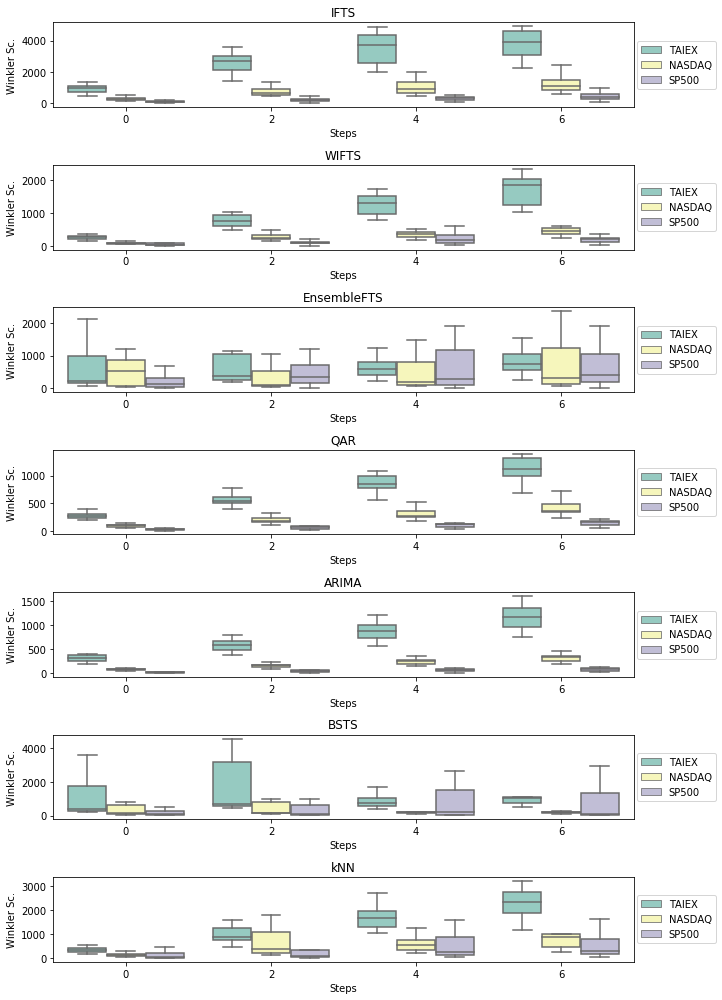
\includegraphics[width=\textwidth]{figures/interval_many_steps.png}
    \caption{Many steps ahead Winkler Score (with $\alpha=.05$) accuracy for each method}
    \label{fig:interval_many_steps}
\end{figure}

%%%%%%%%%%%%%%%%%%%%%%%%%%%%%%%%%%%%%%%%%%%%%%%%%%%%
%
%%%%%%%%%%%%%%%%%%%%%%%%%%%%%%%%%%%%%%%%%%%%%%%%%%%%
\subsection{Probabilistic Forecasting Benchmarks}
\label{sec:prob_experiments_probabilistic}

The CRPS Mean results for each method and dataset are presented in Table \ref{tab:prob_crps_results}. The Friedman Aligned Ranks of the methods are presented on Table \ref{tab:prob_crps_ranks} and the test statistic for these results is $Q = 7.264833574529668$, where the p-Value is $P(\chi ^2_{df} < Q) = 0.12253751253946543$, with $df=4$ degrees of freedom. For this statistic the $H_0$ is accepted at the $\alpha = .05$ confidence level, indicating that there is no difference between the means of the competitor models. This result discards the need to employ \textit{post-hoc} tests and show that there is no prevalence of one method over others. The EnsembleFTS probabilistic forecasting method performed satisfactorily when compared with the standard methods in the literature. 

The statistical tests were employed on the one step ahead forecasts. Figure \ref{fig:probabilistic_many_steps} shows, for each method and dataset, the impact of the forecasting horizon on the CRPS accuracy.

\begin{table}[htp]
    \centering
    \begin{tabular}{|c|ccccc|}
\hline
\textbf{ Dataset } & \textbf{ QAR } & \textbf{ kNN } & \textbf{ ARIMA } & \textbf{ EnsembleFTS } & \textbf{ BSTS } \\
\hline
\multirow{2}{*}{NASDAQ} &    1.028 &    1.158 &    1.444 &       1.923 &    3.208 \\
&  $\pm$ 0.748 &  $\pm$  0.477 &  $\pm$  1.303 &     $\pm$  1.416 &  $\pm$  3.983 \\ \hline
\multirow{2}{*}{TAIEX} &    1.135 &    1.229 &    1.691 &       1.301 &    4.081 \\
 &  $\pm$  0.613 &  $\pm$  0.693 &  $\pm$  1.239 &     $\pm$  1.118 &  $\pm$  5.306 \\ \hline
\multirow{2}{*}{S\&P 500} &    1.557 &    4.403 &    1.216 &       1.995 &    3.278 \\
&   $\pm$  1.74 &  $\pm$  3.261 &  $\pm$  1.166 &     $\pm$  2.255 &   $\pm$  3.16 \\ \hline
\end{tabular}
    \caption{Average CRPS for one step ahead probabilistic forecasts}
    \label{tab:prob_crps_results}
\end{table}

\begin{table}[htb]
    \centering
    \begin{tabular}{llr}
\toprule
METHOD &       RANK \\
\midrule
QAR &   3.000000 \\
ARIMA &   6.666667 \\
kNN &   8.333333 \\
EnsembleFTS &   8.666667 \\
BSTS &  13.333333 \\
\bottomrule
\end{tabular}
    \caption{Friedman Test aligned ranks}
    \label{tab:prob_crps_ranks}
\end{table}

\begin{figure}[htb]
    \centering
    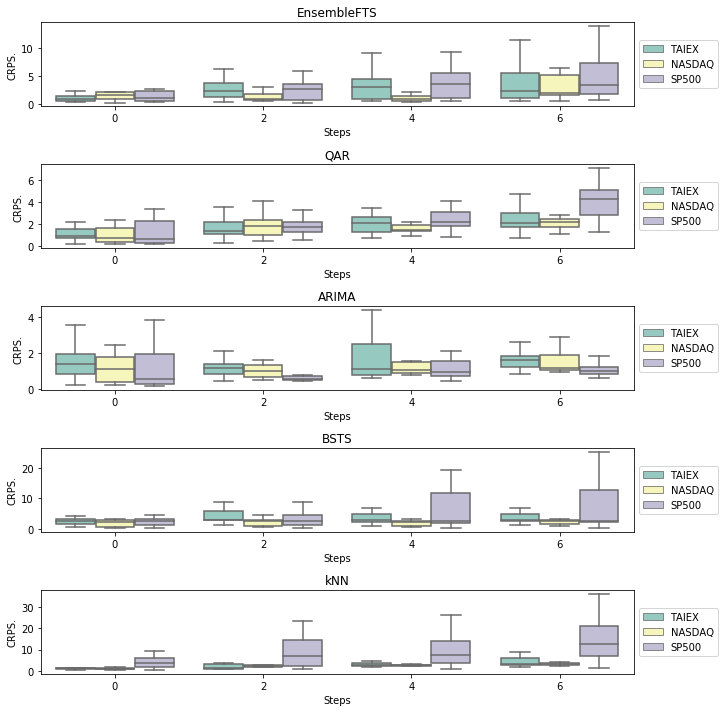
\includegraphics[width=\textwidth]{figures/probabilistic_many_steps.png}
    \caption{Many steps ahead CRPS accuracy for each method}
    \label{fig:probabilistic_many_steps}
\end{figure}


%%%%%%%%%%%%%%%%%%%%%%%%%%%%%%%%%%%%%%%%%%%%%%%%%%%%
%
%%%%%%%%%%%%%%%%%%%%%%%%%%%%%%%%%%%%%%%%%%%%%%%%%%%%
\section{Conclusion}
\label{sec:prob_conclusion}

This chapter provided a brief introduction about point forecasting uncertainties and the main kinds of probabilistic forecasting, reviewing the related literature and proposed new FTS methods for forecasting intervals and probability distributions, which were empirically assessed.

It is remarkable that point forecasts induce to overconfidence and,  without uncertainty measures, point forecasts can be compared to lottery games. It is known that all forecasting models have an irreducible uncertainty term, besides others not-known or not managed uncertainties, and sometimes this information is critical for decision makers.

The Prediction Interval forecasts allow users to assess the uncertainty, delimiting their expected bounds. Probabilistic forecasting methods assist users to know the uncertainty associated with the entire Universe of Discourse. However, these probabilistic forecasting methods can be computationally expensive and time consuming tasks. Also, the cited models were not adapted to deal with fuzzy numbers as input. Neither FTS literature, at this point, presented methods capable to forecast prediction intervals or probability distributions.

To exploit this lack it was proposed the Interval FTS - $\ifts$, the Weighted Interval FTS - $W\ifts$, two new FTS approaches to bind the fuzzy uncertainty of the FTS models, and the Ensemble FTS, the first FTS approach capable to produce probability distributions. In $\ifts$ and $W\ifts$ methods, the prediction interval $\interval$ contains the lower and upper bounds of all fuzzy sets involved on forecasting step, and the length of this interval measure the fuzzy uncertainty.

If $\ifts$ and $W\ifts$ methods deal only with the fuzzy uncertainty, the Ensemble FTS method try to represent the partitioning and ordering uncertainty to produce probabilistic forecasts. The performed computational experiments showed that the accuracy of the intervals and probability distributions provided by the proposed methods do not differ from the standard methods of the literature, showing its reliability.

\subsection{Methods limitations}

The main strength of these methods is their flexibility. This approaches can be used to extend all FTS methods to interval and probabilistic forecasting easily. However, some drawbacks still persist.  $\ifts$ and $W\ifts$ provide intervals, but not probability distributions, and its intervals do not carry a probabilistic uncertainty. Ensemble FTS is few parsimonious and computationally expensive when compared to single FTS methods. An integrated method for point, interval and probabilistic forecasting still is demanded. 

To fix these lacks, in the next chapter a new Fuzzy Time Series method with the ability to  represent epistemic and ontological uncertainty is proposed and their uses for point, interval, and probabilistic forecasting are examined.


\chapter[Probabilistic Weighted Fuzzy Time Series]{Probabilistic Weighted Fuzzy Time Series} 
\index{Probabilistic Weighted Fuzzy Time Series}\index{PWFTS}
\label{chap:pwfts}

\newepigraph{Water is the softest thing, yet it can penetrate mountains and earth. This shows clearly the principle of softness overcoming hardness.}{Lao Tsu}

In this chapter proposes the basic  Probabilistic Weighted Fuzzy Time Series (PWFTS) method, a new FTS method for point, interval and probabilistic forecasting for one to many steps ahead. The PWFTS method aims to produce forecasts by dealing with two sources of uncertainty: fuzzy measurements and stochastic behavior. The fuzziness is induced for a data reduction purpose, in a process that reminds a simple bin discretization. The stochastic behavior is deduced by the  frequentist approach over the previous fuzzyfication. 

Regarding to Chapter \ref{chap:review_fts} fuzzy time series architectural chooses, the PWFTS method is a  time invariant and heuristic method to produce probabilistic weighted rules model $\model$. This method embodied all explored hyperparameters but their definition involves more complex optimization methods, that will be explored in Chapter \ref{chap:scalability}. Default values were defined for hyperparameters, except $k$ and $\Omega$ which must be determined by the user, as shown in Table \ref{tab:pwfts_hyperparam}. These values, however, can be overridden by user. 

\begin{table}[htb] 
    \centering
    \begin{tabular}{|c|c|} \hline
        \textbf{Parameter} & \textbf{Default Value}  \\ \hline
        $\Omega$ & User defined  \\ \hline
        $k$ & User defined  \\ \hline
        $\Pi$ & Grid \\ \hline
        $\mu$ & triangular  \\ \hline 
        $\alpha$-cut & 0 \\ \hline
        $L$ & $\{1,\ldots,\Omega\}$  \\ \hline
    \end{tabular}
    \caption{PWFTS hyperparameter default values}
    \label{tab:pwfts_hyperparam}
\end{table}

The option for a weighted rule knowledge model has the objective to help in the human readability and model explainability, also other knowledge extraction tasks. The weighted rule model will also help, as it will be seen in next chapters, in the distributed processing of the method and on its multivariate extension.

\index{Probabilistic Weighted Fuzzy Logical Relationship Groups}\index{PWFLRG}

The model rules (the Probabilistic Weighted FLRG's) describe the most probable future behavior (the $RHS$ - right hand side of the rule) given some past behavior (the $LHS$ - left hand side of the rule). For a given data sample there will be  many applicable rules with different activations (the membership weights) and all of them are taken into account.

The conception of this method mix the statistical approach of time series forecasting with the FTS techniques. Given some stochastic process $Y$, their best predictor is given by the conditional expectation $\mathbb{E}[y(t+1)\ |\ y(t),...]$. The FTS methods, especially that ones based on \cite{chen1996forecasting}, try to represent the behavior of $Y$ process by splitting their UoD in overlapping fuzzy sets, fuzzyfying the crisp data $Y$ to transform it on the fuzzy time series $F$ and identifying the sequential patterns.  The fuzzy sets are used to define zones, or fuzzy states, at the universe of discourse which have a common set of rules. That's what FLRGs really are: rules that describe sequential patterns. 

Then, for a given FLRG with form $LHS \rightarrow RHS$, where $F(t-1) = LHS$ and $F(t) \in RHS$ our best predictor can be rewritten from $\mathbb{E}[F(t+1)\ |\ F(t),...]$ to $\mathbb{E}[RHS|LHS]$.  The weights assigned to these rules are the frequentist probabilities of the fuzzy sets, measured during the training phase. 

Regarding the concepts introduced at Chapter \ref{chap:review_probforecasting}, the PWFLRG can be seen as a representation of a discrete empirical probability distribution.  The $RHS$ weights represent the conditional probability $P(A_i\ |\ LHS)$, $\forall A_i \in RHS$ and the $LHS$ weights represents the unconditional \textit{a priori} probabilities of the fuzzy sets. With the midpoints of each fuzzy set and their probabilities is possible then to compute the conditional expectation as a forecast for $F(t+1)$.

In next sections this mechanism is detailed, starting in Section \ref{sec:pwfts_empiricalprob} which discuss the basics of the fuzzy empirical probabilities. In Section \ref{sec:pwfts_training} the training procedure for first order model is presented, and on Section \ref{sec:pwfts_forecasting} the one step ahead method for probabilistic, interval and point forecasting is presented. Section \ref{sec:pwfts_extensions} presents extensions for high-order models and many steps ahead forecasting. On Section \ref{sec:pwfts_experiments} computational experiments are performed to asses the performance of the model and finally, on Section \ref{sec:pwfts_conclusion}, the main features of the proposed method are synthesized.  

%%%%%%%%%%%%%%%%%%%%%%%%%%%%%%%%%%%%%%%%%%%%%%%%%%%%%%%%%%%%%%%%%%%%%%
\section{Fuzzy Empirical Probabilities}
\label{sec:pwfts_empiricalprob}

%Given a univariate time series $Y(t) = \{y(0), y(1), ..., y(n)\}$, where $y(i) \in \mathbb{R}\ \forall i \in t$, $t \in [0, n]$ is the time index and the Universe of Discourse is defined by $U = [\min Y(t),\; \max Y(t)]$. Over $U$ is defined a linguistic variable $F$, with $p$ linguistic terms $A_i$ represented by overlapping fuzzy sets represented by their membership functions $\mu_{A_i}:\mathbb{R} \rightarrow [0,1]$.

%A Fuzzy Time Series $F(t)$ is a transformation of $Y(t)$ using the linguistic variable $F$. $F(t) = \{ f(0), f(1),..., f(n) \}$ where $f(i) = \{ \mu_{A_0}(y(i)), ..., \mu_{A_p}(y(i)) \}\ \forall i \in t$. $F(t)$ can also be represented by the linguistic values instead of the membership values, just by defining $f(i) = \{ A_k |  \mu_{A_k}(y(i)) > 0 \}\ \forall k \in [0,p]\ \forall i \in t$.

The core concept of PWFTS is the fuzzy empirical probability, used to compute the weights of the model, whose intuition is discussed in this section. The initial Zadeh's proposition of fuzzy probability, $P(A) = E[\mu_A]$, proposed in \cite{Zadeh1968}, demands the previous knowledge of the probability distribution over the universe of discourse. Once this distribution for $Y$ is unknown, an empirical distribution must take place. The simplest definition of empirical probability is the relative frequency of a discrete value or of a range of continuous values. Fuzzy Theory provides a different look at traditional Probability Theory because it affects the way the events are counted. On fuzzy sets the notion of event is more complex because the same value can belong to several sets with different degrees of membership, as shown in Figure \ref{fig:pwfts_fuzzyfrequency}. In that case, instead of accounting the integral (i.e. unary) occurrence of the event, their partial occurrence is accounted as the membership value. This method is known by fuzzy frequency, and was firstly  developed in \cite{Luo2000}. A related formulation can be found in \cite{Perfilieva2006}, with the concept of F-Transform, which decomposes the original domain of the time series into fuzzy frequencies over the fuzzy sets. This decomposition can also recreate the time series using the inverse transform. 

Given the sample space $U$ and the fuzzy sets $\ulvar$ over $U$, the partition function $Z_{\ufset}$, $\forall \ufset \in \ulvar$, is the integral of the membership function $\mu_{\ufset}$ over the sample space $U$, such that $Z_{\ufset} = \int_U \mu_{\ufset}(y) dy$ or the discrete approximation $Z_{\ufset} = \sum_{y \in U} \mu_{\ufset}(y)$. With the $Z_{\ufset}$ it is possible to approximate the empirical probability of a fuzzy set $\ufset \in \ulvar$ as the sum of its memberships $\mu_{\ufset}(y)$, $\forall y \in U$ divided by the sum of the partition functions $Z_{\ufset}$ of all fuzzy sets $\ufset \in \ulvar$, as presented in Equation \eqref{eqn:prob_conj_fuzzy}. 

\begin{equation}
P(\ufset) = \frac{\sum_{y \in U} \mu_{\ufset}(y)}{\sum_{\ufset \in \ulvar}Z_{\ufset}} 
\label{eqn:prob_conj_fuzzy}
\end{equation}

\begin{figure}
    \centering
    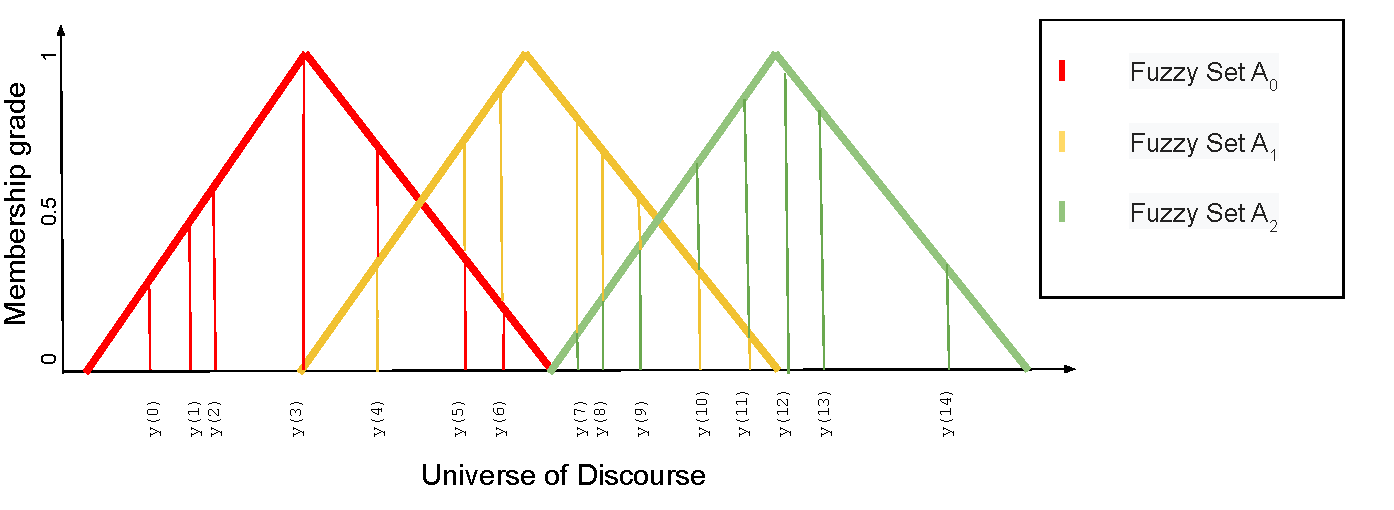
\includegraphics[width=\textwidth]{figures/pwfts_fuzzyfrequency.pdf}
    \caption{Fuzzy frequencies of each $y(t) \in Y$ used to approximate the fuzzy empirical probabilities $P(A_i)$ for each fuzzy set $A_i$}
    \label{fig:pwfts_fuzzyfrequency}
\end{figure}

The intuition behind this equation is that the empirical probability $P(\ufset)$ is evenly spread over the shape of the fuzzy membership function $\mu_{\ufset}$, and the point $y$ is a slice of this shape whose area is equal to the value $\mu_{\ufset}(y)$ (as shown in Figure \ref{fig:pwfts_fuzzyfrequency}), and the area of $\mu_{\ufset}$ is $Z_{\ufset}$. $P(A_i)$ is measured from a sample of $Y$, and this empirical value is an approximation of the true (but unknown) probability. This approximation is used in \eqref{eqn:prob_fuzzy} to approximate the conditional probability of a value $y \in U$, given a fuzzy set $\ufset \in \ulvar$:

\begin{equation}
P(y | \ufset) = P(\ufset) \cdot \frac{\mu_{\ufset}(y)}{Z_{\ufset}}
\label{eqn:prob_fuzzy}
\end{equation}

Using \eqref{eqn:prob_conj_fuzzy} and \eqref{eqn:prob_fuzzy} and the Law of Total Probability the empirical probability $P(y)$ can be approximated using the Equation \eqref{eqn:total_probability}. 

\begin{equation}
P(y,\ulvar) = \sum_{\ufset \in \ulvar} P(y | \ufset)\cdot P(\ufset)
\label{eqn:total_probability}
\end{equation}

The advantage of this approach is the convenience to obtain $P(\ufset)$ from a sample of the time series dataset $Y$. The accuracy of $P(\ufset)$ is determined mainly by $k$, the number of partitions of the universe of discourse $U$.


%%%%%%%%%%%%%%%%%%%%%%%%%%%%%%%%%%%%%%%%%%%%%%%%%%%%%%%%%%%%%%%%%%%%%%%%%%%%%%%%%
\section{PWFTS Training procedure}
\label{sec:pwfts_training}

The training procedure is a seven step method that learn the temporal dynamics of the time series training data $Y$ and represent it on a fuzzy-probabilistic model, namely the Probabilistic Weighted Fuzzy Temporal Rule - PWFTPG. The steps of the method are listed below :

\begin{enumerate}
\item[Step 1] \textit{Define the universe of discourse}: Define $U$ as the sample space of in-sample training data $Y$, such that $U = [\min(Y) - D_1, \max(Y)+D_2]$, where $[\min(Y), \max(Y)]$ is the range of in-sample data and $D_1$ and $D_2$ are numbers used to extrapolate this range, for instance $D_1 = 0.1\cdot\min(Y)$ and $D_2 = 0.1\cdot\max(Y)$;

\item[Step 2] \textit{Partitioning}: split $U$ in $k$ even length intervals $u_i$, for $i = 1,\ldots,k$, with midpoints $mp_i$;

\item[Step 3] \textit{Define the linguistic variable $\ulvar$}: Create $k$ overlapping fuzzy sets $\ufset$, with membership functions $\mu_{\ufset}$, related to an interval $u_j$, and midpoints $mp_j$. Each fuzzy set $\ufset \in \ulvar$ is a linguistic term of the linguistic variable $\ulvar$;

\item[Step 4] \textit{Fuzzyfication}: Transform the original numeric time series $Y$ into the FTS $F$, whose each data point $f(t) \in F$ is a $k$-tuple with the membership value of $y(t)$ with respect to each linguistic term $\ufset \in \ulvar$, such that:

\begin{equation}
f(t) = \left[\mu_{A_1}(y(t)),\ \mu_{A_2}(y(t)),\ \ldots,\ \mu_{A_k}(y(t)) \right]
\end{equation}

\item[Step 5] \textit{Generate the FTP set}: The Fuzzy Temporal Pattern - FTP\footnote{This nomenclature is adopted in replacement of Fuzzy Logical Relationships (FLR) used in \cite{song1993fuzzy}, to avoid misunderstandings with the terms ``logical" and ``relationship" with their classical meanings in fuzzy theory literature.} is a fuzzy rule with format $A_i \rightarrow A_k$ that indicates a temporal succession where the precedent (or the Left Hand Side - LHS) is $A_i \in f(t)$ and the consequent (or the Right Hand Side - RHS) is $A_k \in f(t+1)$, for each possible pair of $A_i \times A_k$ of membership values greater than zero, i.e.,  $\{A_i \rightarrow A_k\}$ $\forall A_i \in f(t)\ |\ \mu_{A_i}(y(t)) > 0$ and $\forall A_k \in f(t+1)\ |\ \mu_{A_k}(y(t+1)) > 0 $. . Therefore, $A_i \rightarrow A_k$ can be read as ``IF $y(t)$ is $A_i$ THEN $y(t+1)$ is $A_k$".
As each $f(t) \in F$ is a sparse $k$-vector of membership values, there will be many possible fuzzy sets combinations of two sequential vectors $f(t)$ and $f(t+1)$. Then for each sequential pair on $F$ possibly more than one FTP will be generated;

\item[Step 6] \textit{Generate the FTPG set}: A Fuzzy Temporal Pattern Group - FTPG\footnote{In replacement of Fuzzy Logical Relationship Group - FLRG used in \cite{Chen2006}.} represents the set of all FTPs with the same LHS and the union of their RHS, with the format $A_i \rightarrow A_k, A_j,...$, where the LHS is $f(t) = A_i$ and the RHS is $f(t+1) \in \{A_k, A_j,...\}$. Each FTPG can be understood as the set of possibilities which may happen at time $t+1$ (the consequent) when a certain set $A_i$ is identified at time $t$ (the precedent).

\item[Step 7] \textit{Calculate empirical probabilities}: The Probabilistic Weighted FTPG - PWFTPG adds weights on the LHS and the RHS that measure their fuzzy empirical probabilities. Each PWFTPG has the format $\pi_j \cdot A_j \rightarrow  w_{j0} \cdot A_0, ..., w_{jk} \cdot A_k$ for $j = 1,\ldots, k$. The set of all  PWFTPG, shown in \eqref{eqn:ftpg}, form the model $\model$. Its size depends on the number of partitions $k$, and it could be represented in matrix form but the weights $w_{ij}$ form a very sparse matrix, which justifies using optimized data structures for its representation.

\begin{equation}
\begin{array}{rcl}
\pi_1 \cdot A_1 & \rightarrow &  w_{11} \cdot A_1, ..., w_{1k} \cdot A_k \\
\ldots & \ldots & \ldots \\
\pi_k \cdot A_k & \rightarrow &  w_{k1} \cdot A_1, ..., w_{kk} \cdot A_k
\end{array}
\label{eqn:ftpg}
\end{equation}

Each weight $\pi_i$ is associated with the fuzzy set in the LHS of the rule, and it is the normalized sum of all LHS memberships of all FTPs where the LHS is the fuzzy set $\ufset$, as in \ref{eqn:prob_conj_fuzzy}. $\pi_i$ can be understood as the empirical \textit{a priori} probability of the fuzzy set $\ufset$ independent of time, or $P(\ufset)$, such that the condition of Equation \ref{eqn:apriori_condition} must be satisfied for the PWFTPG set in \ref{eqn:ftpg}.

\begin{equation}
    \sum_{j \in \ulvar} \pi_i = 1
    \label{eqn:apriori_condition}
\end{equation}

Each weight $w_{ji}$ is associated with a fuzzy set $\ufset$ on the RHS of the FTP whose the LHS is $\ufset$, and it is the normalized sum of all RHS memberships of all FTPs where $LHS = \ufset$ and $RHS = A_i$. Therefore, the weight $w_{ji}$ can be understood as the empirical conditional probability of the fuzzy set $A_i$ on time $t+1$ when the fuzzy set $\ufset$ is identified on time $t$, or $P(A_i^{t+1}\ |\ \ufset^t)$, such that the condition of Equation \ref{eqn:aposteriori_condition} must be satisfied for each $\ufset$ in LHS.

\begin{equation}
    \sum_{i \in \ulvar} w_{ji} = 1 \quad \forall \ufset \in \ulvar
    \label{eqn:aposteriori_condition}
\end{equation}


\end{enumerate}

The outcome of the Training Procedure is the PWFTPG set and it represents the temporal dynamics of the original data. It is an empirical probability distribution of the linguistic variable $A$ over the time series $Y$ with sample space $U$, where each rule contains the unconditional probability $P(\ufset) = \pi_j$ and conditional probabilities $P(A_i | \ufset) = w_{ji}$, for $A_i,A_j \in \ulvar$.

\begin{figure}
    \centering
    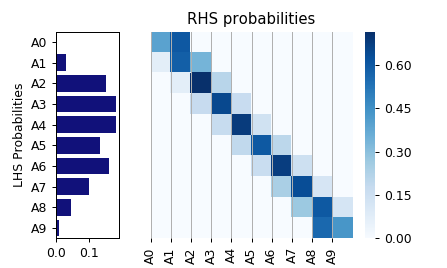
\includegraphics{figures/pwfts_rules_firstorder.png}
    \caption{Representation of first order PWFTPG ruleset}
    \label{fig:pwfts_rules_firstorder}
\end{figure}


%%%%%%%%%%%%%%%%%%%%%%%%%%%%%%%%%%%%%%%%%%%%%%%%%%%%%%%%%%%%%%%%%%%%%%%%%%%%%%%%%
\section{Forecasting Procedure}
\label{sec:pwfts_forecasting}

The forecasting procedure is a four step procedure listed in this section, which takes as input the forecasting type, a sample $y(t) \in U$ and uses the PWFTPG model $\mathcal{M}$ learned in the previous section to generate the output, which depends on the type of forecasting  (probabilistic, interval or point forecasting).  The complete forecasting procedure is presented below:

\begin{enumerate}
\item[Step 1] \textit{Fuzzyfication}: For a given input value $y(t) \in Y$, find the fuzzyfied values $f(t) = \{\ufset \ |\ \mu_{\ufset}(y(t)) > \alpha\}$;
\item[Step 2] \textit{Pattern matching}:  Locate all the PWFTPG's whose the LHS is $f(t)$.
\item[Step 3] \textit{Forecast}: The distribution of $f(t+1)$ is given by the RHS sets of each PWFTPG matched;
\item[Step 4] \textit{Defuzzyfication}: 
\begin{enumerate}
    \item If the forecasting type is Probabilistic, then build the probability distribution $P(y(t+1) | y(t))$, $\forall y(t+1) \in U$ applying Equation \ref{eqn:pwfts_probabilistic} presented in Section \ref{sec:pwfts_probabilistic};
    \item If the forecasting type is Interval, then build the prediction interval $\intvl(t+1)$ applying Equation \ref{eqn:pwfts_interval} presented in Section \ref{sec:pwfts_interval};
    \item If the forecasting type is Point, then build the crisp estimate $\estimate$ applying Equation \ref{eqn:pwfts_point} presented in Section \ref{sec:pwfts_point};
\end{enumerate}

\end{enumerate}


%%%%%%%%%%%%%%%%%%%%%%%%%%%%%%%%%%%%%%%%%%%%%%%%%%%%%%%%%%%%%%%%%%%%%%%%%%%%%%%%%
\subsection{Probabilistic Forecasting Procedure}
\label{sec:pwfts_probabilistic}

A probability distribution $P( y(t+1) | y(t))$, for all  $y(t+1) \in U$ can be computed using a Mixture Distribution approach to transform each PWFTPG probability into a continuous distribution, as described in Equation \ref{eqn:pwfts_probabilistic}.

A mixture distribution is defined as $P(y) = \sum \omega_j \cdot \pi_j(y)$ where $\pi_j: U \rightarrow [0,1]$ are specific PDFs and $\omega_j$ is a weight associated to each PDF, such that $\sum \omega_j = 1$. Given an input value $y(t) \in Y$ and the PWFTPG set, the probability distribution for each $y(t+1) \in U$ is given by \eqref{eqn:pwfts_probabilistic}, where $\omega_j$ is replaced by the probability $P(y(t)|A_i)$, the LHS probability given the input value, and the distribution $\pi_j$ is replaced by the probability $P(y(t+1)|A_j,A_i)$, $\forall A_j \in RHS$. 

Looking back to Equation \ref{eqn:prob_fuzzy}, it is clear that $\sum_{\ufset \in  \ulvar} P(y(t)|\ufset) < 1$, once $P(A_i)$ is the probability of the whole fuzzy set and $y(t)$ is just a small slice of it, thus it does not comply with the $\sum \omega_j = 1$ restriction of the mixture distribution. To work around this issue $P(y(t)|\ufset)$ is re-scaled using the Equation \ref{eqn:pwfts_rescaling}.

\begin{equation}
\frac{P(y(t)|\ufset)}{\sum_{\ufset \in \ulvar} P(y(t)|\ufset)}      
\label{eqn:pwfts_rescaling}
\end{equation}

Therefore, the final conditional probability $P(y(t+1) | y(t))$,  given the linguistic variable $\ulvar$ and a PWFTPG set $\model$, is defined in Equation \ref{eqn:pwfts_probabilistic}. A sample of the PWFTS probabilistic forecasting for one step ahead can be seen in Figure \ref{fig:pwfts_sample_manystep}.

\begin{equation}
\begin{array}{cl}
P(y(t+1) | y(t)) &=  \displaystyle \sum_{\ufset \in  \ulvar}\frac{\displaystyle P(y(t)| \ufset) \left( \sum_{i = 1}^k  P(y(t+1) | A_i,\ufset) \right)}{\displaystyle \sum_{i = 1}^k P(y(t)| A_i)}  \\
& \\
 &= \displaystyle \sum_{\ufset \in  \ulvar} \frac{ \displaystyle  \pi_j\frac{\mu_{\ufset}(y(t))}{Z_{\ufset}} \left( \sum_{i = 1}^k  w_{ji}\frac{\mu_{A_i}(y(t+1))}{Z_{A_i}} \right)}{\displaystyle \sum_{i = 1}^k \pi_i\frac{\mu_{A_i}(y(t))}{Z_{A_i}}}
\end{array}
\label{eqn:pwfts_probabilistic}
\end{equation}

\begin{figure}
    \centering
    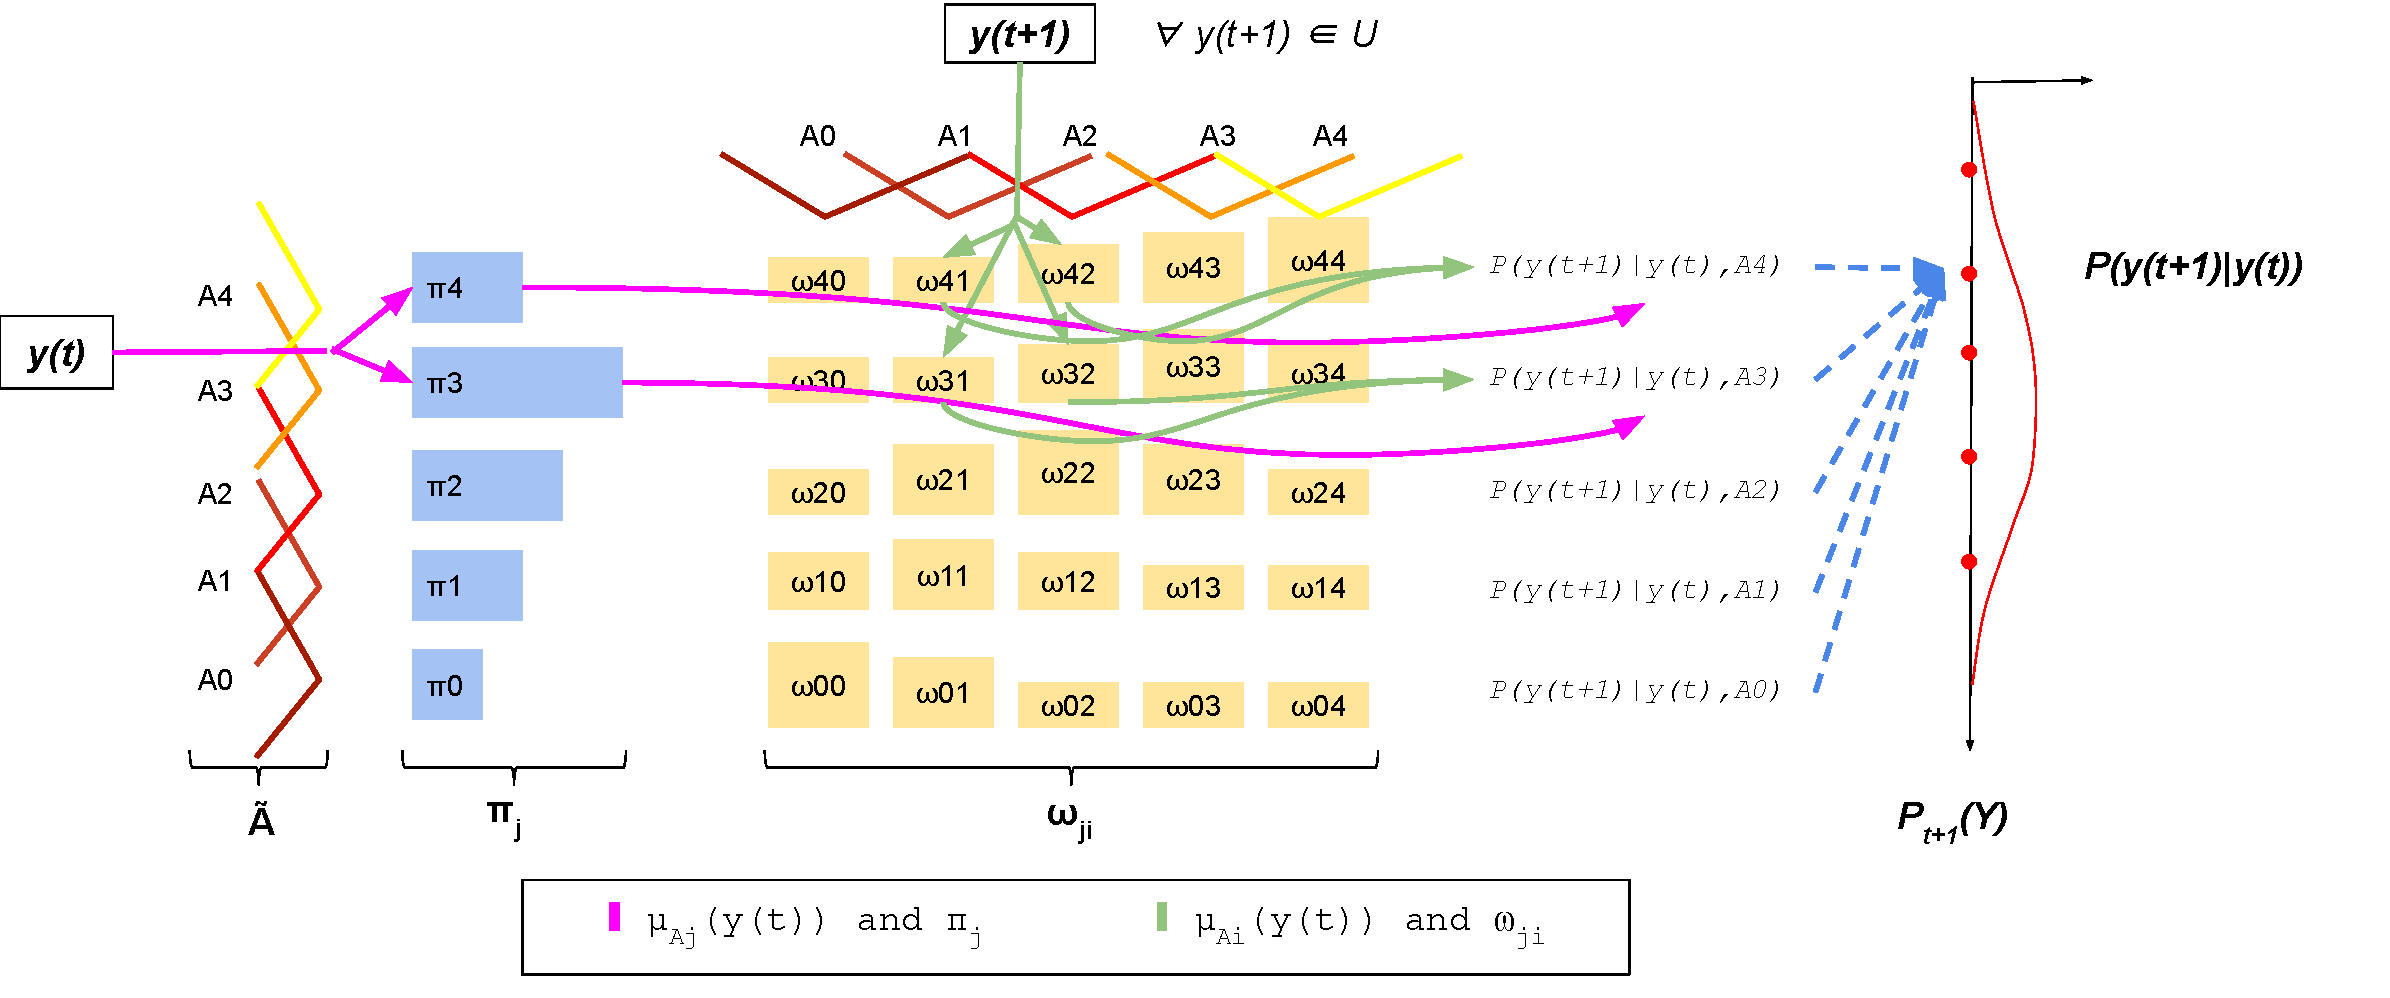
\includegraphics[width=\textwidth,height=7cm]{figures/pwfts_probabilistic_forecasting.pdf}
    \caption{Representation of PWFTS probabilistic forecasting procedure, where the length of blue boxes represents the magnitude of $\pi_j$ weights and the height of yellow boxes represents the magnitude of $\omega_{ji}$ weights.}
    \label{fig:pwfts_probabilistic_forecasting}
\end{figure}

\begin{figure}[htb]
    \centering
    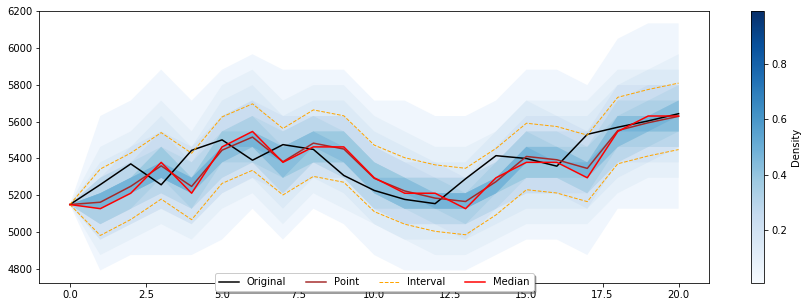
\includegraphics[width=\textwidth]{figures/pwfts_sample_onestep.png}
    \caption{Sample of PWFTS for one step ahead forecasting}
    \label{fig:pwfts_sample_onestep}
\end{figure}

\begin{figure}[htb]
    \centering
    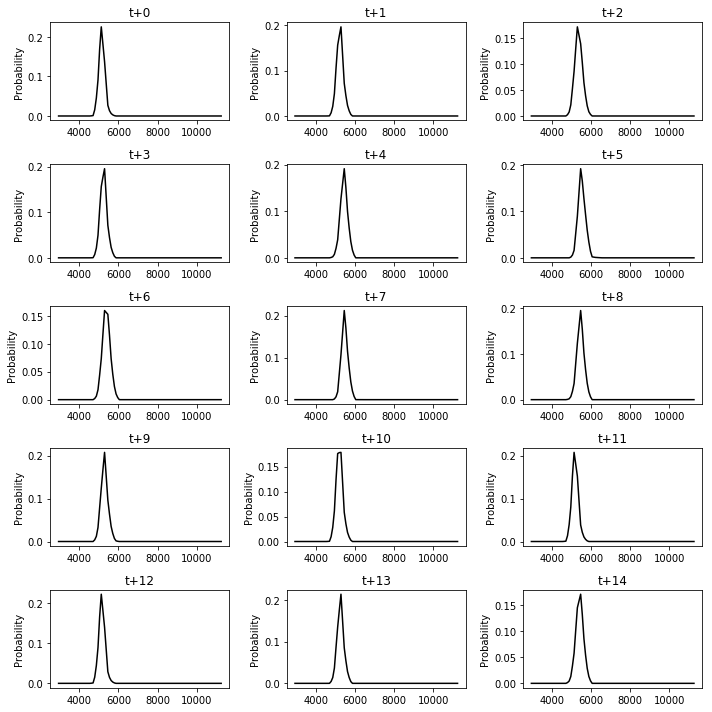
\includegraphics[width=\textwidth]{figures/pwfts_sample_onestep_tiled.png}
    \caption{Shapes of PWFTS probability distributions for one step ahead forecasting}
    \label{fig:pwfts_sample_onestep_tiled}
\end{figure}

%%%%%%%%%%%%%%%%%%%%%%%%%%%%%%%%%%%%%%%%%%%%%%%%%%%%%%%%%%%%%%%%%%%%%%%%%%%%%%%%%
\subsection{Interval forecasting procedure}
\label{sec:pwfts_interval}

A forecasting interval $\intvl (t+1)$ can be produced from $P( y(t+1) | y(t))$, once it is possible to build a cumulative density function $F( y(t+1) | y(t))$ and use it to construct the quantile function $Q(\tau): [0,1] \rightarrow U$, as shown in Equation \ref{eqn:quantile_function} where $\tau \in [0,1]$ is the desired quantile. Then, for a certain confidence level $\alpha \in [0,1]$, it is possible to compute an inter quantile interval $\mathbb{I}_f = [\underline{Q(\alpha)}, \overline{Q(1 - \alpha)}]$.

\begin{equation}
Q(\tau) = \min\{x \in U\ |\ F(x | y(t)) = \tau \}
\label{eqn:quantile_function}
\end{equation}

However, the above method demands the previous computation of the whole probability density function $P( y(t+1) | y(t))$, which is computationally expensive for larger input samples. A simpler and faster heuristic for generating prediction intervals extend the method $W\ifts$, proposed in Section \ref{sec:wifts}, to exploit the structure of the PWFTPG weights. Each PWFTPG will be represented by an interval $\intvl$ whose bounds are the expectation of the bounds of its RHS fuzzy sets, such that $\underline{\ufset}$ and $\overline{\ufset}$ represent the lower and upper bounds of the fuzzy set $\ufset$, and $\mathbb{E}[ \ufset ]$ is the expectation of the PWFTPG where the LHS is $\ufset$. The forecasting interval  $\intvl(t+1)$ then is the sum of these expectations weighted by the $P(y(t)|\ufset)$ probabilities, as presented in Equation \ref{eqn:pwfts_interval}. A sample of the PWFTS interval forecasting for one step ahead can be seen in Figure \ref{fig:pwfts_sample_manystep}.

\begin{equation}
\begin{array}{rcl}
\intvl_j & = & \displaystyle [\underline{\mathbb{E}[ \ufset ]}\ ,\ \overline{\mathbb{E}[ \ufset ]}] \\
\underline{\mathbb{E}[ \ufset ]} & = & \sum_{A_i \in \ufset^{RHS}} w_{ji}\cdot \underline{A_i} \\ 
\overline{\mathbb{E}[ \ufset ]} & = & \sum_{A_i \in \ufset^{RHS}} w_{ji}\cdot \overline{A_i}
\end{array}
\end{equation}

\begin{equation}
\begin{array}{rcl}
\mathbb{I}(t+1) & = & \displaystyle [\underline{\mathbb{E}[ \ulvar | y(t) ]}\ ,\ \overline{\mathbb{E}[ \ulvar | y(t) ]}] \\
& & \\
& = & \displaystyle \left[\frac{\sum_{\ufset \in \ulvar} P(y(t)|\ufset)\cdot \underline{\intvl_j}}{\sum_{\ufset \in \ulvar} P(y(t)|\ufset)},\frac{\sum_{\ufset \in \ulvar} P(y(t)|\ufset)\cdot \overline{\intvl_j}}{\sum_{\ufset \in \ulvar} P(y(t)|\ufset)}\right]
\end{array}
\label{eqn:pwfts_interval}
\end{equation}

%%%%%%%%%%%%%%%%%%%%%%%%%%%%%%%%%%%%%%%%%%%%%%%%%%%%%%%%%%%%%%%%%%%%%%%%%%%%%%%%%
\subsection{Point forecasting procedure}
\label{sec:pwfts_point}

To produce point forecasts $\estimate$ from the existing distribution $P(\cdot|y(t))$ it is only needed to apply the expectation operator, such that $\estimate = \mathbb{E}[P(y(t+1)|y(t))]$. This is also computationally expensive due to the computation of $P(y(t+1)|y(t))$. A simple heuristic for producing point forecasts is to compute the expectation $\mathbb{E}[\ufset]$ of each PWFTPG, as presented in Equation \ref{eqn:pwftpg_expectation}, where $mp_i$ is the midpoint of each fuzzy set $A_i \in RHS$. The expectation $\mathbb{E}[\ufset]$ for each PWFTPG $\ufset$ is constant and can be pre-computed. The final forecast $\estimate$ then is the sum of these expectations weighted by $P( y(t) | \ufset)$ probability, as shown in Equation \ref{eqn:pwfts_point}. A sample of the PWFTS point forecasting for one step ahead can be seen in Figure \ref{fig:pwfts_sample_manystep}.

\begin{equation}
\mathbb{E}[ \ufset ] = \displaystyle \sum_{i \in \ufset^{RHS}} w_{ji}\cdot mp_i
\label{eqn:pwftpg_expectation}
\end{equation}

\begin{equation}
\estimate = \displaystyle \mathbb{E}[ \ulvar | y(t) ] =  \sum_{\ufset \in \ulvar} \frac{ P(y(t) | \ufset) \cdot \mathbb{E}[ \ufset ]} { \sum_{\ufset \in \ulvar} P(y(t) | \ufset)}
\label{eqn:pwfts_point}
\end{equation}

%%%%%%%%%%%%%%%%%%%%%%%%%%%%%%%%%%%%%%%%%%%%%%%%%%%%%%%%%%%%%%%%%%%%%%%%%%%%%%%%%%%%%%%
%%%%%%%%%%%%%%%%%%%%%%%%%%%%%%%%%%%%%%%%%%%%%%%%%%%%%%%%%%%%%%%%%%%%%%%%%%%%%%%%%%%%%%%

\section{PWFTS extensions}
\label{sec:pwfts_extensions}

In the next subsections the basic first-order and one-step-ahead method is extended to higher orders and wider forecasting horizons in order to increase PWFTS method flexibility and versatility.

%%%%%%%%%%%%%%%%%%%%%%%%%%%%%%%%%%%%%%%%%%%%%%%%%%%%%%%%%%%%%%%%%%%%%%%%%%%%%%%%%%%%%%%
\subsection{Many steps ahead forecasting}
\label{sec:pwfts_many_step}

The forecasting procedures listed in Section \ref{sec:pwfts_forecasting} are one step ahead methods. To extend the forecasting procedures to many steps ahead forecasting, an iterative approach is adopted, in which the $t+1$ step is computed with the previously presented methods and its output is fed back as input to the next $H$ steps. From the step $t+2$ on, let $h \in [t+2, t+H]$ be the new time indexer. The simpler approach is to perform the point forecast of $y(h+1)$  with the input $y(h)$.

The interval procedure requires a few more modifications. Given the input $\intvl(h)$ the same interval forecasting procedure will be executed with inputs $\underline{\intvl(h)}$ and $\overline{\intvl(h)}$ producing two new intervals $\underline{\intvl(h+1)}$ and $\overline{\intvl(h+1)}$. Then the final forecasting interval will be $\intvl(h+1) = [\min\{\underline{\intvl(h+1)}\}, \max\{\overline{\intvl(h+1)}\}]$. 

Finally, the probabilistic forecasting for $P(y(h+1)|y(h))$ given the input will change to  \ref{eqn:extension_probabilistic}, instead of \ref{eqn:pwfts_probabilistic}. This equation replaces $P(y(h) | \ufset)$ for the previous probability distribution $P(y(h)|y(h-1))$. A sample of the PWFTS many steps ahead forecasting can be seen in Figure \ref{fig:pwfts_sample_manystep}.

%\begin{equation}
%\medmath{
%P(y(s+1) | y(s))  = \frac{\sum_{i = 1}^k %P(y(s)| y(s-1))\cdot \left(  \sum_{j = 1}^k  %P(y(s+1) | A_j,A_i) \right)}{\sum_{i = 1}^k %P(y(s)| y(s-1))}}
%\label{eqn:extension_probabilistic}
%\end{equation}

\begin{equation}
P(y(h+1) | y(h))  = \displaystyle \sum_{\ufset \in \ulvar} \frac{ P(y(h)| y(h-1), \ufset)}{ \sum_{i = 1}^k P(y(h)| y(h-1), A_i)} \times  \left(  \sum_{z = 1}^k  P(y(h+1) | A_z,\ufset) \right)
\label{eqn:extension_probabilistic}
\end{equation}

\begin{figure}
    \centering
    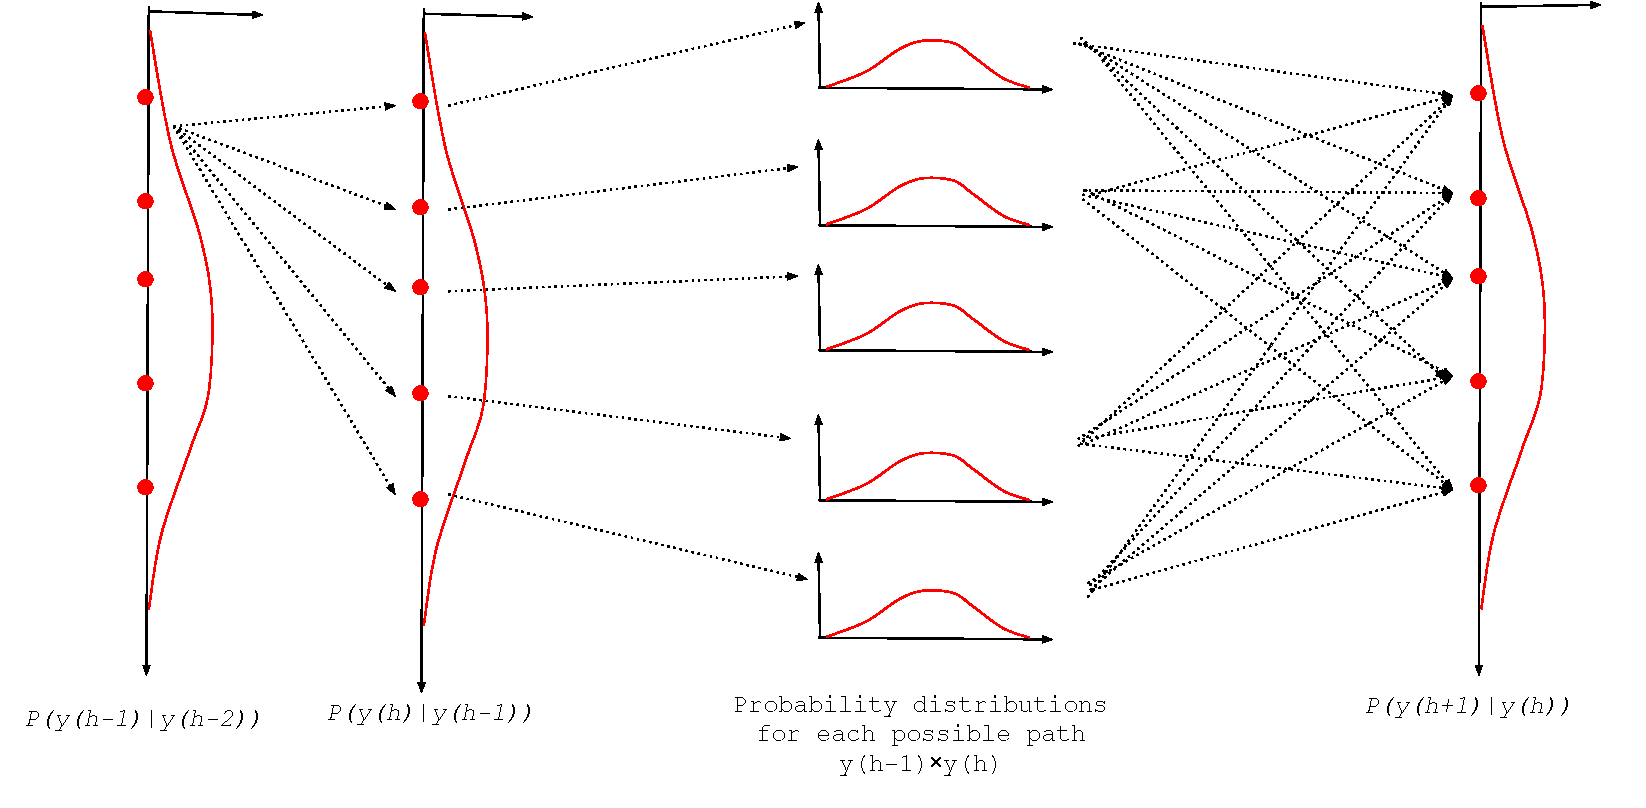
\includegraphics[width=\textwidth]{figures/pwfts_probabilistic_manysteps.pdf}
    \caption{Caption}
    \label{fig:pwfts_probabilistic_manysteps}
\end{figure}
 
\begin{figure}[htb]
    \centering
    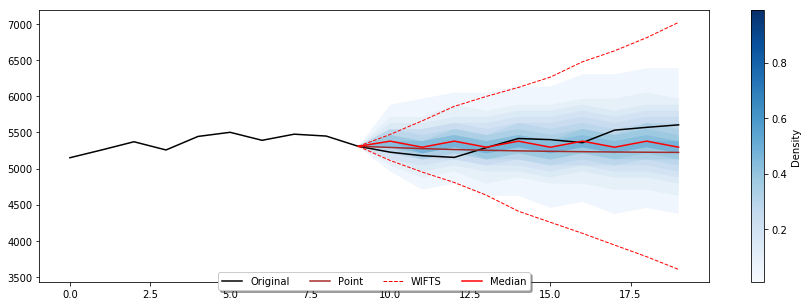
\includegraphics[width=\textwidth]{figures/pwfts_sample_manystep.png}
    \caption{Sample of PWFTS for 7 step ahead forecasting}
    \label{fig:pwfts_sample_manystep}
\end{figure}

\begin{figure}[htb]
    \centering
    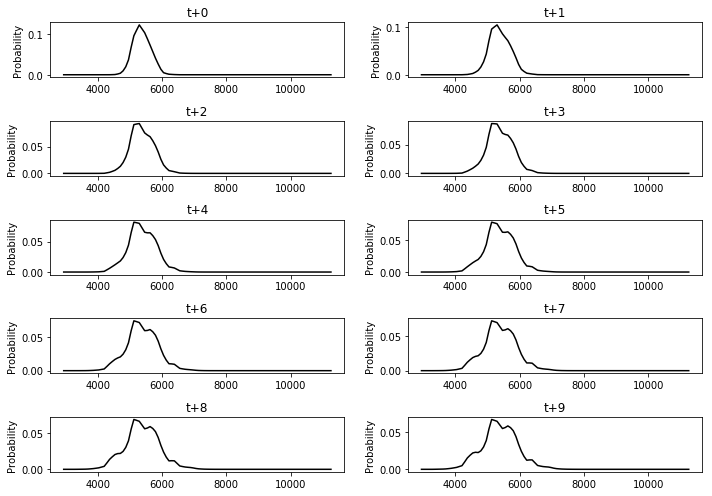
\includegraphics[width=\textwidth]{figures/pwfts_sample_manystep_tiled.png}
    \caption{Shapes of PWFTS probability distributions for many steps ahead forecasting}
    \label{fig:pwfts_sample_manystep_tiled}
\end{figure}

%%%%%%%%%%%%%%%%%%%%%%%%%%%%%%%%%%%%%%%%%%%%%%%%%%%%%%%%%%%%%%%%%%%%%%%%%%%%%%%%%%%%%%%
\subsection{High order models}
\label{sec:pwfts_high_order}

The PWFTS method described in Section \ref{sec:pwfts_training} is a first order method, i.e., it just needs $y(t)$ to forecast $\estimate$, while high order models use $\Omega$ time lags, whose indexes are stored on vector $L$. To extend the standard approach to high order  modification in Step 5 of the Training procedure is needed to adapt the FTPs and FTPGs to store $\Omega$ fuzzy sets on their LHS.

Once the fuzzyfied value $f(t)$ has multiple fuzzy sets (with different membership values greater than $alpha$-cut), a set of fuzzyfied values $f(t-L(\Omega)),...,f(t-L(0))$ must be represented with all possible combinations between the fuzzy sets of each lag, such as $f(t-L(\Omega)) \times f(t - L(\Omega-1)) \times \ldots \times f(t-L(0))$, where $\times$ represents the Cartesian Product operator. 

In Step 5 the FTPs will have the format $\ufset^{L(\Omega)}, \ufset^{L(\Omega-1)},\ldots,\ufset^{L(0)} \rightarrow A_i$, which can be read as ``IF $f(t-L(\Omega))$ is $\ufset^{L(\Omega)}$ AND $f(t-L(\Omega-1))$ is $\ufset^{L(\Omega-1)}$ AND $\dots$ AND $f(t-L(0))$ is $\ufset^{L(0)}$ THEN $f(t+1)$ is $A_i$". In Step 6, the high order FTPGs gather all high order FTPs with the same LHS. 

In Step 7 the $\pi_j$ weight is replaced by $\pi_{LHS}$ that aggregates the $\mu_{LHS}$ memberships of each FTPG for the samples. Given a sample $y(t-\Omega),\dots,y(t) \in Y$ with $\Omega$ lags, their membership grades with a FTPG is the product T-norm between all memberships of the LHS: 

\begin{equation}
\displaystyle  \mu_{LHS}(y(t-L(\Omega)),\ldots,y(t-L(0)) = \bigcap_{i = \Omega}^0 \mu_{\ufset}(y(t-L(i)))
\label{eqn:extension_highorder_mu}
\end{equation}

In the forecasting procedure, the Step 1 requires a sample with $\Omega$ lags that will generate $\Omega$ fuzzyfied values. In Step 2, all combinations between the fuzzy sets of each fuzzyfied lag will be the LHS of the affected PWFTPGs. In Step 3, in Equations \ref{eqn:pwfts_probabilistic}, \ref{eqn:pwfts_interval} and \ref{eqn:pwfts_point}, the empirical conditional probability $P(y(t)|A_i)$ will be replaced by $P(y(t-m),...,y(t) | LHS)$, the empirical conditional probability of the sample $y(t-m),...,y(t)$ given the LHS of the PWFTPG.

\begin{equation}
\displaystyle P(y(t-L(\Omega))\ldots y(t-L(0) | LHS) = \pi_{LHS} \frac{\mu_{LHS}(y(t-L(\Omega))\ldots,y(t-L(0))}{\sum_{\ufset \in LHS} Z_{\ufset}}
\label{eqn:extension_highorder}
\end{equation}


%%%%%%%%%%%%%%%%%%%%%%%%%%%%%%%%%%%%%%%%%%%%%%%%%%%%%%%%%%%%%%%%%%%%%%%%%%%%%%%%%%%%%%%
%%%%%%%%%%%%%%%%%%%%%%%%%%%%%%%%%%%%%%%%%%%%%%%%%%%%%%%%%%%%%%%%%%%%%%%%%%%%%%%%%%%%%%%

\section{Computational Experiments}
\label{sec:pwfts_experiments}

In this section presents an empirical study of the PWFTS performance using the same datasets, design of experiments and statistical tests employed in Sections \ref{sec:fts_experiments} and \ref{sec:prob_experiments}. PWFTS method can forecast points, intervals, and probability distributions, then the following sections will present all these compared results.

To measure the performance of the proposed models were chosen ARIMA, QAR, kNN/KDE, and BSTS as competitor models due to its possibility to perform point, interval and probabilistic forecasting for many steps ahead. The hyperparameters of each method were individually investigated and only the best model is taken account on the validation of the results. The HOFTS and WHOFTS methods were also used to compare the point forecasts, using the best models determined in Section \ref{sec:fts_experiments}. The $\ifts$ and $W\ifts$ methods were also used to compare the interval forecasts, and EnsembleFTS was also used to compare probabilistic forecasts, using the best models determined in Section \ref{sec:prob_experiments}.

In Section \ref{sec:pwfts_hyperparameters}, the accuracy sensitivity regarding to the hyperparameters of the proposed methods are analyzed using a grid search. The result of the experiments are presented in Sections \ref{sec:pwfts_experiments_point} for point forecasting, \ref{sec:pwfts_experiments_interval} for interval forecasting  and  \ref{sec:prob_experiments_probabilistic}, for probabilistic forecasting.

In order to contribute with the replication of all the results in the research, all data and source codes employed in this chapter are available at the URL:
\texttt{\url{http://bit.ly/scalable_probabilistic_fts_chap4}}

%%%%%%%%%%%%%%%%%%%%%%%%%%%%%%%%%%%%%%%%%%%%%%%%%%%%%%%%%%%%%%%%%%%%%%%%%%%%%%%%%%%%%%%
%%%%%%%%%%%%%%%%%%%%%%%%%%%%%%%%%%%%%%%%%%%%%%%%%%%%%%%%%%%%%%%%%%%%%%%%%%%%%%%%%%%%%%%
\subsection{Hyperparameter Grid Search}
\label{sec:pwfts_hyperparameters}

In order to asses the impact of the hyperparameters on PWFTS accuracy, a Search Grid was performed for each benchmark dataset, using the same search spaces contained on Table \ref{tab:ifts_gridsearch} of Section \ref{sec:prob_hyperparameters}. But, different from the previous experiments this grid search was performed for point, interval and probabilistic forecasting, in order to chose the hyperparameter values that best fit all cases.

The RMSE accuracy is shown on Figure \ref{fig:pwfts_gridsearch_point}, by order, number of partitions and dataset. The Winkler Score accuracy, where  $\alpha \in \{.05,.25\}$, can be observed on Figure \ref{fig:pwfts_gridsearch_interval} and the CRPS accuracy on Figure \ref{fig:pwfts_gridsearch_probabilistic}.

Once several numbers of partitions and order values achieved very closed accuracy values, the Principle of Parsimony (or Occam's Razor) was adopted to chose the set of hyperparameters that leads to smallest number of rules $|\model|$, keeping the same accuracy. The chosen hyperparameters were $k = 45$ and $\Omega = 1$ and a sample of the best models performance can be seen in Figure \ref{fig:pwfts_sample_onestep} (for one step ahead) and \ref{fig:pwfts_sample_manystep} (for many steps ahead).


\begin{figure}[htb]
    \centering
    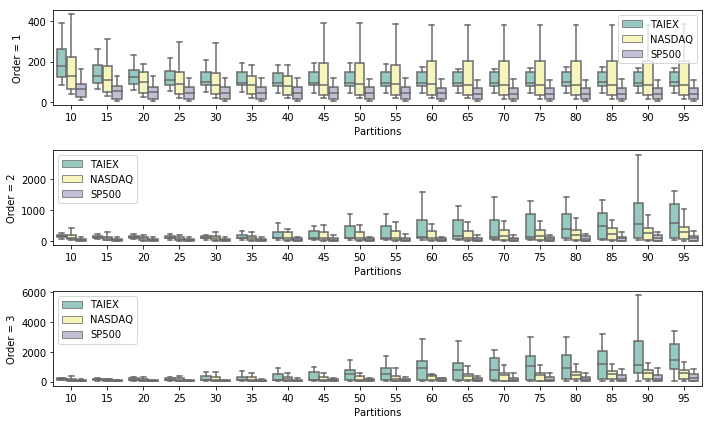
\includegraphics[width=\textwidth,height=12cm]{figures/pwfts_gridsearch_point.png}
    \caption{RMSE accuracy for order, partitions and dataset}
    \label{fig:pwfts_gridsearch_point}
\end{figure}

\begin{figure}[htb]
    \centering
    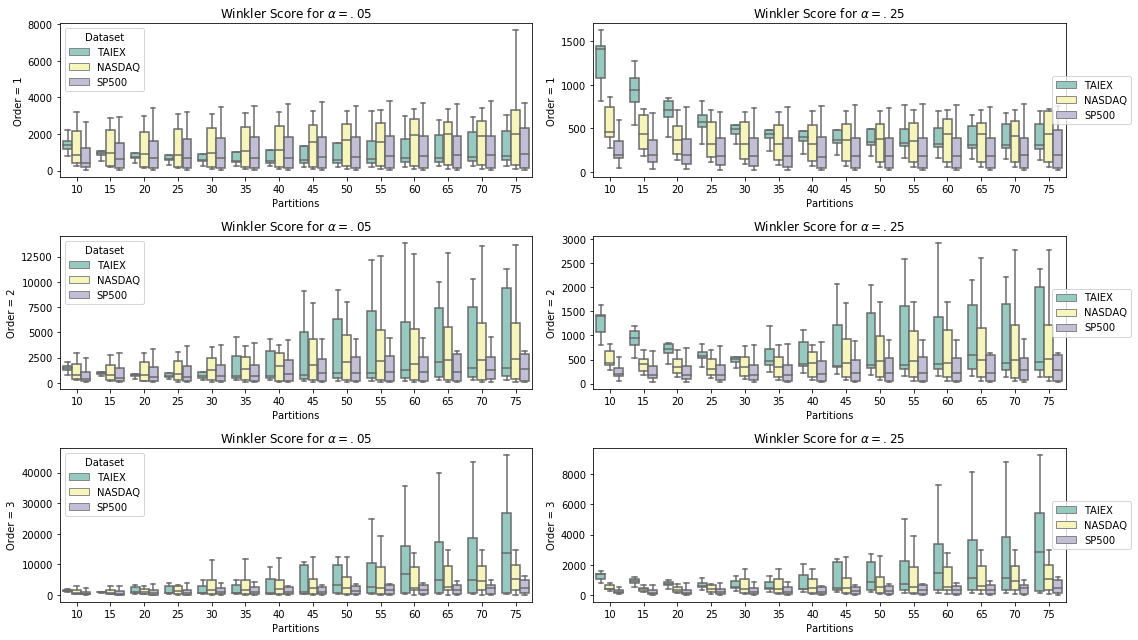
\includegraphics[width=\textwidth,height=12cm]{figures/pwfts_gridsearch_interval.png}
    \caption{Mean Winkler Score for $\alpha \in \{.05,.25\}$ by order, partitions and dataset}
    \label{fig:pwfts_gridsearch_interval}
\end{figure}

\begin{figure}[htb]
    \centering
    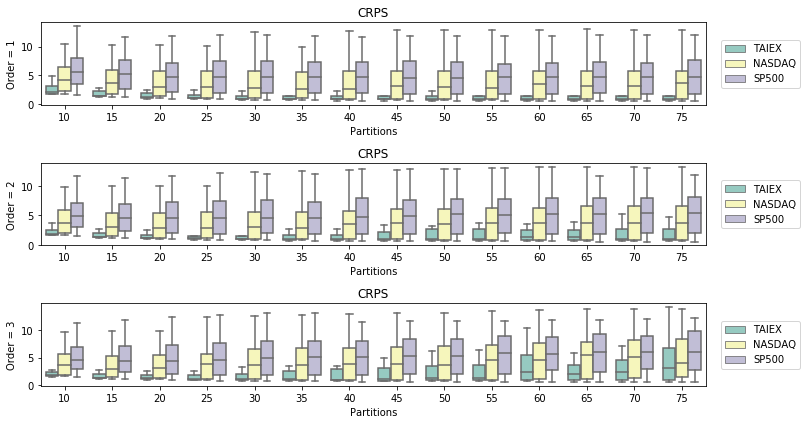
\includegraphics[width=\textwidth]{figures/pwfts_gridsearch_probabilistic.png}
    \caption{CRPS accuracy by order, partitions and dataset}
    \label{fig:pwfts_gridsearch_probabilistic}
\end{figure}


%%%%%%%%%%%%%%%%%%%%%%%%%%%%%%%%%%%%%%%%%%%%%%%%%%%%%%%%%%%%%%%%%%%%%%%%%%%%%%%%%%%%%%%
%%%%%%%%%%%%%%%%%%%%%%%%%%%%%%%%%%%%%%%%%%%%%%%%%%%%%%%%%%%%%%%%%%%%%%%%%%%%%%%%%%%%%%%
\subsection{Point Forecasting Benchmarks}
\label{sec:pwfts_experiments_point}

The RMSE results for each method and dataset are presented on Table \ref{tab:pwfts_point_results}. The Friedman Aligned Ranks of the methods are presented in Table \ref{tab:prob_interval_ranks} and the test statistic for these results is $Q = 13.903114186851207$, where the p-value is $P(\chi^2_{df} < Q) = 0.030737356514312197$, with $df=7$ degrees of freedom. For this statistic the $H_0$ is rejected at the $\alpha=.05$ confidence level, indicating that there is difference between the means of the competitor models.

The \textit{post-hoc} tests were employed using PWFTS as control methods and their results are presented on Table \ref{tab:pwfts_point_posthoc}, showing that there is no prevalence of PWFTS method over all others. The mean difference detected by the Friedman Test occurred between QAR and BSTS, where QAR prevails over BSTS with p-value of 0.006984, rejecting $H_0$ of \textit{post-hoc} tests. These results showed that PWFTS point forecasting method perform satisfactorily when compared with the standard methods in the literature. 

The statistical tests were employed to one step ahead forecasts. Figure \ref{fig:pwfts_ahead_point} shows, for each method and dataset, the impact of the forecasting horizon on the RMSE accuracy.

\begin{table}[ht]
\resizebox{\textwidth}{!}{% <------ Don't forget this %
\centering
    \begin{tabular}{|c|ccccccc|}
\hline
\textbf{Dataset} & \textbf{ARIMA} & \textbf{QAR} & \textbf{PWFTS} & \textbf{WHOFTS} & \textbf{HOFTS} & \textbf{kNN} & \textbf{BSTS} \\
\hline
\multirow{2}{*}{S\&P 500} &     6.091 &     8.177 &    10.541 &    12.822 &    13.605 &    19.242 &    380.466 \\
 &   $\pm$7.452 &  $\pm$11.366 &   $\pm$10.19 &  $\pm$11.336 &  $\pm$12.392 &   $\pm$24.97 &  $\pm$947.809 \\ \hline
\multirow{2}{*}{NASDAQ} &    22.592 &    17.951 &    24.839 &    27.154 &    29.713 &    34.742 &    413.494 \\
 &  $\pm$24.991 &  $\pm$11.965 &  $\pm$18.198 &   $\pm$15.05 &  $\pm$12.875 &  $\pm$25.096 &  $\pm$837.281 \\ \hline
\multirow{2}{*}{TAIEX} &    91.311 &      66.9 &    75.558 &    90.433 &   100.787 &    80.213 &     271.66 \\
 &  $\pm$63.249 &  $\pm$44.369 &  $\pm$56.739 &   $\pm$58.93 &  $\pm$62.932 &  $\pm$56.494 &  $\pm$250.078 \\ \hline
\end{tabular}
}
    \caption{RMSE for one step ahead point forecasts}
    \label{tab:pwfts_point_results}
\end{table}

\begin{table}[hbt]
    \centering
    \begin{tabular}{|c|c|}
\hline
       METHOD &       RANK \\
\hline
QAR &   6.333333 \\
ARIMA &   7.333333 \\
PWFTS &   8.333333 \\
WHOFTS &  10.333333 \\
HOFTS &  12.000000 \\
kNN &  12.666667 \\
BSTS &  20.000000 \\
\hline
\end{tabular}
    \caption{Friedman aligned ranks for point forecasts}
    \label{tab:pwfts_point_ranks}
\end{table}

\begin{table}[htb]
\resizebox{\textwidth}{!}{% <------ Don't forget this %
    \centering
    \begin{tabular}{llrrrl}
\toprule
{} &       COMPARISON &   Z-VALUE &   P-VALUE &  ADJUSTED P-VALUE &       Result \\
\midrule
0 &    PWFTS vs BSTS &  2.302831 &  0.021288 &          0.121122 &  H0 Accepted \\
1 &     PWFTS vs kNN &  0.855337 &  0.392364 &          0.775648 &  H0 Accepted \\
2 &   PWFTS vs HOFTS &  0.723747 &  0.469221 &          0.775648 &  H0 Accepted \\
3 &     PWFTS vs QAR &  0.394771 &  0.693012 &          0.829909 &  H0 Accepted \\
4 &  PWFTS vs WHOFTS &  0.394771 &  0.693012 &          0.829909 &  H0 Accepted \\
5 &   PWFTS vs ARIMA &  0.197386 &  0.843526 &          0.843526 &  H0 Accepted \\
\bottomrule
\end{tabular}
}
    \caption{Post-hoc tests using PWFTS as control method}
    \label{tab:pwfts_point_posthoc}
\end{table}

\begin{figure}[htb]
    \centering
    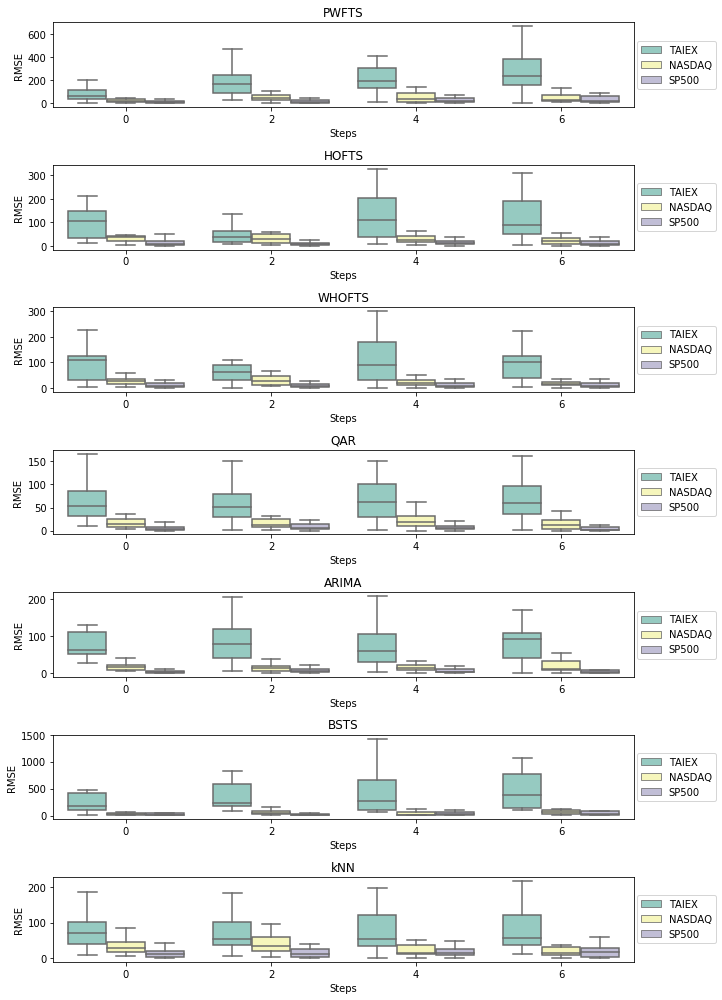
\includegraphics[width=\textwidth]{figures/pwfts_ahead_point.png}
    \caption{Impact of the forecasting horizon on RMSE accuracy}
    \label{fig:pwfts_ahead_point}
\end{figure}

%%%%%%%%%%%%%%%%%%%%%%%%%%%%%%%%%%%%%%%%%%%%%%%%%%%%%%%%%%%%%%%%%%%%%%%%%%%%%%%%%%%%%%%
%%%%%%%%%%%%%%%%%%%%%%%%%%%%%%%%%%%%%%%%%%%%%%%%%%%%%%%%%%%%%%%%%%%%%%%%%%%%%%%%%%%%%%%
\subsubsection{Residual Analysis}
\label{sec:pwfts_residual}

The residuals of the models are presented in Figures \ref{fig:pwfts_residual} and the Ljung-Box tests for the 3 first lags are presented in Table \ref{tab:pwfts_residual} , which is shown the good fit of the model. 

\begin{figure}[h]
    \centering
    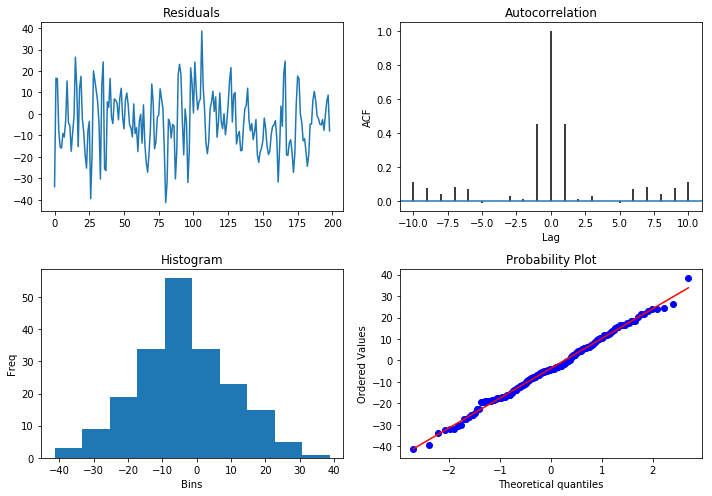
\includegraphics[width=\textwidth,height=7cm]{figures/pwfts_residual.png}
    \caption{Residual analysis of PWFTS}
    \label{fig:pwfts_residual}
\end{figure}

\begin{table}[htb]
    \centering
\begin{tabular}{lrrrrl}
\toprule
Lag &  Statistic &       p-Value &  Critical Value &       Result \\
\midrule
1 &  34.846143 &  3.568157e-09 &        3.841459 &  H0 accepted \\
2 &  35.497255 &  1.958254e-08 &        5.991465 &  H0 accepted \\
3 &  35.871542 &  7.971605e-08 &        7.814728 &  H0 accepted \\
\bottomrule
\end{tabular}
    \caption{Ljung-Box Test for the 3 first lags}
    \label{tab:pwfts_residual}
\end{table}

%%%%%%%%%%%%%%%%%%%%%%%%%%%%%%%%%%%%%%%%%%%%%%%%%%%%%%%%%%%%%%%%%%%%%%%%%%%%%%%%%%%%%%%
%%%%%%%%%%%%%%%%%%%%%%%%%%%%%%%%%%%%%%%%%%%%%%%%%%%%%%%%%%%%%%%%%%%%%%%%%%%%%%%%%%%%%%%
\subsection{Interval Forecasting Benchmarks}
\label{sec:pwfts_experiments_interval}

The Winkler Score Mean results for each method and dataset are presented on Table \ref{tab:pwfts_interval_results}. The Friedman Aligned Ranks of the methods are presented in Table \ref{tab:pwfts_interval_ranks} and the test statistic for these results is $Q = 14.812664$, where the p-Value is $P(\chi^2_{df} < Q) = 0.038477$, with $df=7$ degrees of freedom. For this statistic, the $H_0$ is rejected at the $\alpha=.05$ confidence level, indicating that there is a difference between the means of the competitor models.

The \textit{post-hoc} tests were employed using PWFTS as control methods and their results are presented in Table \ref{tab:pwfts_interval_posthoc}, showing the prevalence of PWFTS over BSTS. These results showed that PWFTS interval forecasting methods perform satisfactorily when compared with other standard methods in the literature. 

The statistical tests were employed on the one-step ahead forecasts. Figure \ref{fig:pwfts_ahead_interval} shows, for each dataset, the impact of the forecasting horizon on the Winkler Score accuracy of PWFTS.


\begin{table}[h]
\resizebox{\textwidth}{!}{% <------ Don't forget this %
\centering
\begin{tabular}{|c|cccccccc|}
\hline
\textbf{Dataset} & \textbf{ARIMA} & \textbf{PWFTS} & \textbf{QAR} & \textbf{WIFTS} & \textbf{IFTS} & \textbf{kNN} & \textbf{EnsembleFTS} & \textbf{BSTS} \\ \hline
\multirow{2}{*}{S\&P 500} &      72.712 &    73.505 &    121.694 &    111.705 &    113.516 &    131.394 &     268.567 &     292.415 \\
 &   $\pm$135.871 &   $\pm$99.09 &  $\pm$319.305 &  $\pm$156.013 &   $\pm$91.627 &   $\pm$166.31 &   $\pm$318.259 &   $\pm$384.499 \\ \hline
\multirow{2}{*}{NASDAQ} &     233.261 &   112.944 &    106.416 &     123.35 &    284.692 &    170.709 &     603.881 &     652.036 \\
 &   $\pm$486.735 &  $\pm$33.666 &   $\pm$56.248 &  $\pm$141.251 &   $\pm$147.24 &  $\pm$156.097 &   $\pm$638.297 &   $\pm$963.624 \\ \hline
\multirow{2}{*}{TAIEX} &     858.124 &   348.647 &        340 &    480.581 &    917.879 &    428.484 &     898.531 &     1280.67 \\
 &  $\pm$1337.139 &  $\pm$82.036 &   $\pm$269.34 &  $\pm$561.826 &  $\pm$243.737 &  $\pm$269.459 &  $\pm$1175.107 &  $\pm$1472.031 \\ \hline
\end{tabular}
}
    \caption{Average Winkler Score with $\alpha=.05$ for one step ahead interval forecasts}
    \label{tab:pwfts_interval_results}
\end{table}

\begin{table}[hbt]
    \centering
    \begin{tabular}{|c|c|}
\hline
       METHOD &       RANK \\
\hline
PWFTS &   6.000000 \\
QAR &   6.666667 \\
WIFTS &   7.666667 \\
kNN &   8.666667 \\
ARIMA &  13.000000 \\
IFTS &  16.666667 \\
EnsembleFTS &  19.666667 \\
BSTS &  21.666667 \\
\hline
\end{tabular}
    \caption{Friedman aligned ranks for interval forecasts }
    \label{tab:pwfts_interval_ranks}
\end{table}

\begin{table}[htb]
\resizebox{\textwidth}{!}{% <------ Don't forget this %
    \centering
\begin{tabular}{llrrrl}
\toprule
{} &            COMPARISON &   Z-VALUE &   P-VALUE &  ADJUSTED P-VALUE &       Result \\
\midrule
0 &         PWFTS vs BSTS &  2.713546 &  0.006657 &          0.045677 &  H0 Rejected \\
1 &  PWFTS vs EnsembleFTS &  2.367136 &  0.017926 &          0.061349 &  H0 Accepted \\
2 &         PWFTS vs IFTS &  1.847521 &  0.064672 &          0.144442 &  H0 Accepted \\
3 &        PWFTS vs ARIMA &  1.212436 &  0.225346 &          0.360355 &  H0 Accepted \\
4 &          PWFTS vs kNN &  0.461880 &  0.644167 &          0.764634 &  H0 Accepted \\
5 &        PWFTS vs WIFTS &  0.288675 &  0.772830 &          0.822550 &  H0 Accepted \\
6 &          PWFTS vs QAR &  0.115470 &  0.908073 &          0.908073 &  H0 Accepted \\
\bottomrule
\end{tabular}
}
    \caption{Post-hoc tests using PWFTS as control method}
    \label{tab:pwfts_interval_posthoc}
\end{table}

\begin{figure}[htb]
    \centering
    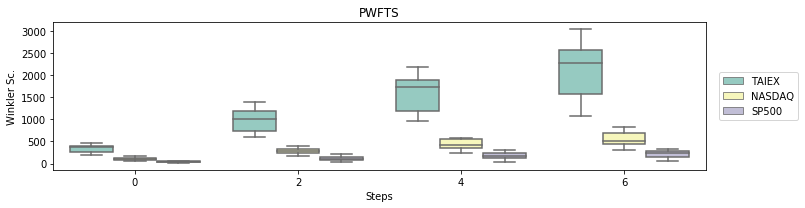
\includegraphics[width=\textwidth]{figures/pwfts_ahead_interval.png}
    \caption{Impact of the forecasting horizon on Winkler Score accuracy}
    \label{fig:pwfts_ahead_interval}
\end{figure}

%%%%%%%%%%%%%%%%%%%%%%%%%%%%%%%%%%%%%%%%%%%%%%%%%%%%%%%%%%%%%%%%%%%%%%%%%%%%%%%%%%%%%%%
%%%%%%%%%%%%%%%%%%%%%%%%%%%%%%%%%%%%%%%%%%%%%%%%%%%%%%%%%%%%%%%%%%%%%%%%%%%%%%%%%%%%%%%
\subsection{Probabilistic Forecasting Benchmarks}
\label{sec:pwfts_experiments_probabilistic}

The CRPS Mean results for each method and dataset are presented in Table \ref{tab:pwfts_probabilistic_results}. The Friedman Aligned Ranks of the methods are presented in Table \ref{tab:pwfts_probabilistic_ranks} and the test statistic for these results is $Q = 10.352711804324706$, where the p-Value is $P(\chi ^2_{df} < Q) = 0.06583635032195168$, with $df=5$ degrees of freedom. For this statistic the $H_0$ is accepted at the $\alpha = .05$ confidence level, indicating that there is no significant difference between the means of the competitor models. This result discards the need to employ \textit{post-hoc} tests and show that there is no prevalence of one method over others, showing also that PWFTS probabilistic forecasting method performed satisfactorily when compared with the standard methods in the literature. 

The statistical tests were employed on the one-step ahead forecasts. Figure \ref{fig:pwfts_ahead_probabilistic} shows, for each dataset, the impact of the forecasting horizon on the CRPS accuracy of PWFTS method.

\begin{table}[h]
\resizebox{\textwidth}{!}{% <------ Don't forget this %
\centering
\begin{tabular}{|c|cccccc|}
\hline
\textbf{Dataset} & \textbf{PWFTS} & \textbf{QAR} & \textbf{kNN} & \textbf{ARIMA} & \textbf{EnsembleFTS} & \textbf{BSTS} \\
\hline
\multirow{2}{*}{NASDAQ} &    0.882 &    1.028 &    1.158 &    1.444 &       1.923 &    3.208 \\
 &  $\pm$0.347 &  $\pm$0.748 &  $\pm$0.477 &  $\pm$1.303 &     $\pm$1.416 &  $\pm$3.983 \\ \hline
\multirow{2}{*}{TAIEX} &    0.967 &    1.135 &    1.229 &    1.691 &       1.301 &    4.081 \\
 &  $\pm$0.404 &  $\pm$0.613 &  $\pm$0.693 &  $\pm$1.239 &     $\pm$1.118 &  $\pm$5.306 \\ \hline
\multirow{2}{*}{S\&P 500} &    1.257 &    1.557 &    4.403 &    1.216 &       1.995 &    3.278 \\
 &  $\pm$0.722 &   $\pm$1.74 &  $\pm$3.261 &  $\pm$1.166 &     $\pm$2.255 &   $\pm$3.16 \\ \hline
\end{tabular}
}
    \caption{CRPS for one step ahead interval forecasts}
    \label{tab:pwfts_probabilistic_results}
\end{table}

\begin{table}[hbt]
    \centering
    \begin{tabular}{|c|c|}
\hline
       METHOD &       RANK \\
\hline
PWFTS &   3.333333 \\
QAR &   5.666667 \\
ARIMA &   8.666667 \\
kNN &  11.333333 \\
EnsembleFTS &  11.666667 \\
BSTS &  16.333333 \\
\bottomrule
\end{tabular}
    \caption{Friedman aligned ranks for probabilistic forecasts }
    \label{tab:pwfts_probabilistic_ranks}
\end{table}

\begin{figure}[htb]
    \centering
    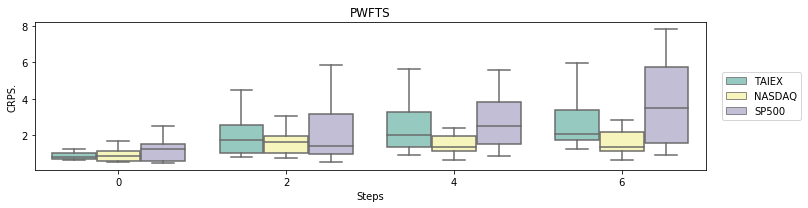
\includegraphics[width=\textwidth]{figures/pwfts_ahead_probabilistic.png}
    \caption{Impact of the forecasting horizon on CRPS accuracy}
    \label{fig:pwfts_ahead_probabilistic}
\end{figure}

%%%%%%%%%%%%%%%%%%%%%%%%%%%%%%%%%%%%%%%%%%%%%%%%%%%%%%%%%%%%%%%%%%%%%%%%%%%%%%%%%%%%%%%
%%%%%%%%%%%%%%%%%%%%%%%%%%%%%%%%%%%%%%%%%%%%%%%%%%%%%%%%%%%%%%%%%%%%%%%%%%%%%%%%%%%%%%%
\section{Conclusion}
\label{sec:pwfts_conclusion}

This chapter proposed a new univariate and time invariant FTS method - the Probabilistic Weighted FTS (PWFTS), a weighted rule-based FTS method which represents their temporal patterns with an empirical probability - based on the proposed concept of fuzzy frequency. The PWFTS rule model - the Probabilistic Weighted Fuzzy Temporal Pattern Groups (PWFTPG) - describes fuzzy and stochastic behavior of time series and combines them to produce forecasts. 

Once was already proposed interval and probabilistic methods, none of them integrate all these capabilities. The strength of PWFTS is its flexibility and performance. This model is used to produce probability densities, prediction intervals and point forecasting, with high order models and multiple-step ahead forecasting.  

Computational experiments were performed to evaluate the accuracy of the proposed model which showed equivalent or better performance than standard methods on literature. Its computational cost is low when compared with BSTS and EnsembleFTS approaches and its interval accuracy is better than WIFTS and IFTS.

The proposed PWFTS method extends FTS methods to deal with interval and probabilistic forecasting applications, which is the major contribution of this research. Moreover, PWFTS improves on former FTS methods in the literature by considering the concept of fuzzy frequency and empirical probabilities in the generation of the rule knowledge base. The proposed method improves previous FTS methods by aggregating probabilistic and interval forecasting capabilities into a single model, being useful for a wide range of applications and user needs.

\subsection{Method limitations}

As in previous FTS methods, the PWFTS accuracy depends on the hyperparameter fine tunning. The method does not embody this optimization and it is advisable that this fine tunning be performed. Another issue about the model optimization is the parsimony: PWFTS weights may vanish as the number of rules increases. The weights precision is limited by the computational numerical precision. 

In general all forecasting procedures are computationally cheap but the probabilistic forecasting for multiple-steps ahead is computationally expensive and the forecasting horizon H must be chosen carefully.

\chapter{Scalability And Hyperparameter Optimization}
\label{chap:scalability}

\newepigraph{While we cannot accurately predict the course of climate change in the coming decades, the risks we run if we don't change our course are enormous. Prudent risk management does not equate uncertainty with inaction.}{Steven Chu}

The previous chapters focused in forecasting tasks and its uncertainties and FTS approaches were presented to deal with theses issues. However, the presented approaches do not optimize its models for a given time series $Y$. The best hyperparameters must be found by the user and then informed to the methods, task that was delegated until now to an expensive Grid Search optimization.

As reviewed in Chapter \ref{chap:review_fts}, several approaches in the literature embody optimization tasks in their training procedures. Nevertheless an holistic hyperparameter optimizer for all FTS components present in Table \ref{tab:fts_hyperparameters} is still lacking in the literature. The most challenging issue presented by this task is the choose of the partitioning method $\Pi$, which may use computationally expensive meta-heuristics (and without known parallel or distributed extensions), and the number of partitions $k$ and order $\Omega$ that regulates the parsimony of the model.

The optimization task becomes even harder when dealing with time series with Big Data properties. Many of the traditional forecasting methods, and even some new ones, were not designed to deal with such high volume of data. The most critical issues are the high dimensionality (dozens of hundreds of attributes) and volume (hundreds of millions or billions of samples), as pointed out in \cite{Qiu2016}. There is not a universal consensus about the small, medium and big data sizes. By simplicity it can be considered that it strongly depends on the available hardware capabilities. 

In all cases Big Data starts to happen when it does not fit in the memory of a single machine. Such data volume, that cannot be grounded on a single machine memory, demands a distributed architecture of storage and processing. New technologies are emerging to tackle these issues, for instance the Map Reduce based frameworks \cite{Dean2008}, a  divide-and-conquer approach which is the basis of Hadoop clusters \cite{White2012}, where the processing units also act as storage units of the data subsets. 

These distributed computation approaches have been determinant to enable the processing of data-intensive and computationally expensive tasks. Thanks to the distributed computation frameworks, soft-computing methods are now enabled to work with massive datasets using cheap and available hardware infrastructure. Such kind of tasks are spread over several areas in science and engineering, such as in weather and environmental datasets and on smart sensor data of smart grids where, according to \cite{Coelho2016}, there are networks of smart sensors continuously monitoring all system components and streaming historical data with high volume and velocity. 

Applying Big Data to machine learning algorithms is a trending topic in recent years, as can be seen in \cite{Zhou2017}. But the literature on taming big time series did not considered FTS methods directly, although there exists approaches involving other fuzzy methods, see for instance \cite{Singh2015}.

The absence of computationally expensive iterative procedures inside the training and forecasting procedures of the proposed FTS methods facilitates its scalability, as well as the use of white box knowledge models that can be easily distributed and updated. With this design, FTS models $\model$ can be quickly trained in commodity hardware, without major processing requirements, and transferred between cluster nodes. 

This chapter aims to propose scalable alternatives to perform  training FTS methods using distributed algorithms and exploit  these solutions to tackle the hyperparameter optimization of big time series. In Section \ref{sec:distributed} an distributed FTS training approach for big time series is proposed. In Section \ref{sec:hyperparameter} the Distributed Evolutionary Hyperparameter Optimization (DEHO) method is proposed, combining evolutionary algorithms and the previously defined distributed training and forecasting approaches. In Section \ref{sec:scalability_experiments} computational experiments are performed to assess the speed up provided by the distributed methods and the convergence of DEHO method for large environmental time series. Finally, in Section \ref{sec:scalability_conclusion} the results are discussed and synthesized.

%%%%%%%%%%%%%%%%%%%%%%%%%%%%%%%%%%%%%%%%%%%%%%%%%%%%%%%%%
%%%%%%%%%%%%%%%%%%%%%%%%%%%%%%%%%%%%%%%%%%%%%%%%%%%%%%%%%
\section{Computational Clusters}

According to \cite{Baker1999}, ``A cluster is a type of parallel or distributed processing system, which consists of a collection of interconnected stand-alone computers working together as a single, integrated computing resource''. Clusters are used for providing high availability, load-balancing, distributed storage, high processing power, among other purposes.

The Distributed Storage Clusters (DSC) systems are employed to keep distributed database systems or distributed file systems, exploiting local storage resources to allow the storage of data volumes that can be handled by a single machine, while providing transparent access to the whole dataset. Diversely, the High Processing Clusters (HPC) systems are employed to solve complex or expensive computational tasks which can be decomposed and parallelized by sub-datasets (Single Instruction / Multiple Data), sub-tasks (Multiple Instruction / Single Data) or both (Multiple Instruction / Multiple Data). A good example of HPC cluster is the classical Beowulf Cluster\footnote{The Beowulf Project - \url{http://www.beowulf.org}. Access in 15/05/2019} architecture, which makes use of message passing middleware like MPI and PVM. In these frameworks the instructions and data are spread across the cluster and, after the local processing on each cluster node finishes, the results are gathered in some master or control node. 

With the advent of Big Data, the demand of distributed file systems capable to store large datasets was joined with the demand for simple programming interfaces for processing distributed data. The Map/Reduce, proposed in \cite{Dean2008}, became a popular distribution paradigm due to its high adoption in Big Data literature. In such paradigm the computational cluster contains a master node, which centralizes the management of the tasks, and several slave nodes responsible for working tasks. The distributed execution is divided into two main phases, the map (scattering) and reduce (gathering). The Map phase splits the original dataset into smaller subsets and distributes them to the slave nodes. Each individual slave node will perform the same predefined set of computations on data and send the results back to the master node. The Reduce phase collects the results from the slave nodes and performs final aggregations of results.

The popularity of the Map/Reduce paradigm to tackle Big Data problems imersed after the first open source infrastructure frameworks became available, for instance Apache Hadoop\footnote{Apache Hadoop Project - \url{https://hadoop.apache.org/}. Access in 15/05/2019}. More recently some infrastructure was developed to allow in-memory processing, turning the processing yet more efficient, as for instance the Spark framework\footnote{Apache Spark - \url{https://spark.apache.org/}. Access in 15/05/2019}. In the next sections, the distribution strategies for the sequential FTS methods are discussed using HPC middleware and Map/Reduce paradigm.


%%%%%%%%%%%%%%%%%%%%%%%%%%%%%%%%%%%%%%%%%%%%%%%%%%%%%%%%%
%%%%%%%%%%%%%%%%%%%%%%%%%%%%%%%%%%%%%%%%%%%%%%%%%%%%%%%%%
\section{Scalable Models With Distributed Execution}
\label{sec:distributed}

Depending on the data size and the capabilities of the available infrastructure, different approaches must be considered for FTS method scalability, specially when dealing with hyperparameter optimization.

Small-sized time series (up to 10,000 instances) can be handled easily by a single machine and the costs of distribution (network and middleware overhead) do not pay off. This is the approach presented in all previous chapters.

For middle sized data (from 10,000 to 500,000 instances) the optimization process is more likely task-intensive, the evaluation dataset $Y$ can be split in smaller train/test data windows that can be handled by a single machine, and just the accuracy results need to be gathered and agregated. This is the approach presented in Section \ref{sec:distributed_testing}.

However, for highly sized data (above 500,000 instances), even the train/test data windows are costly to be trained by a single machine. In this case the training and testing methods need to be distributed themselves. This is the approach presented in Section \ref{sec:distributed_models}.



%%%%%%%%%%%%%%%%%%%%%%%%%%%%%%%%%%%%%%%%%%%%%%%%%%%%%%%%%
%%%%%%%%%%%%%%%%%%%%%%%%%%%%%%%%%%%%%%%%%%%%%%%%%%%%%%%%%
\subsection{Distributed Testing With Sequential Models}
\label{sec:distributed_testing}

The distributed testing with sequential models aims to speed up iterative optimization processes that require unnumbered evaluations of the objective function with different small to medium datasets. Each evaluation requires a sample of the entire dataset with which an FTS model $\model$ will be trained and evaluated using an accuracy metric $\epsilon$.

This is particularly the case of the hyperparameter optimization where, given a set of hyperparameters $\Theta$ and a time series dataset $Y$, for each combination of hyperparameters values $\theta \in \Theta$ being evaluated, it must perform a rolling window cross validation on the time series dataset. The distributed rolling window cross validation, shown in Figure \ref{fig:distributed_testing}, splits the whole dataset $Y$ in $W$ smaller and overlapping data windows $i=1..W$ and each data window is divided in train and test subsets. Then, for each data window $i$, a new model $\model_i$ will be trained and evaluated, generating the local accuracy metric $\epsilon_i$. The average of the accuracy metric is calculated as $\epsilon = W^{-1} \sum_{i=1}^W \epsilon_i$.

\begin{figure}[htb]
    \centering
    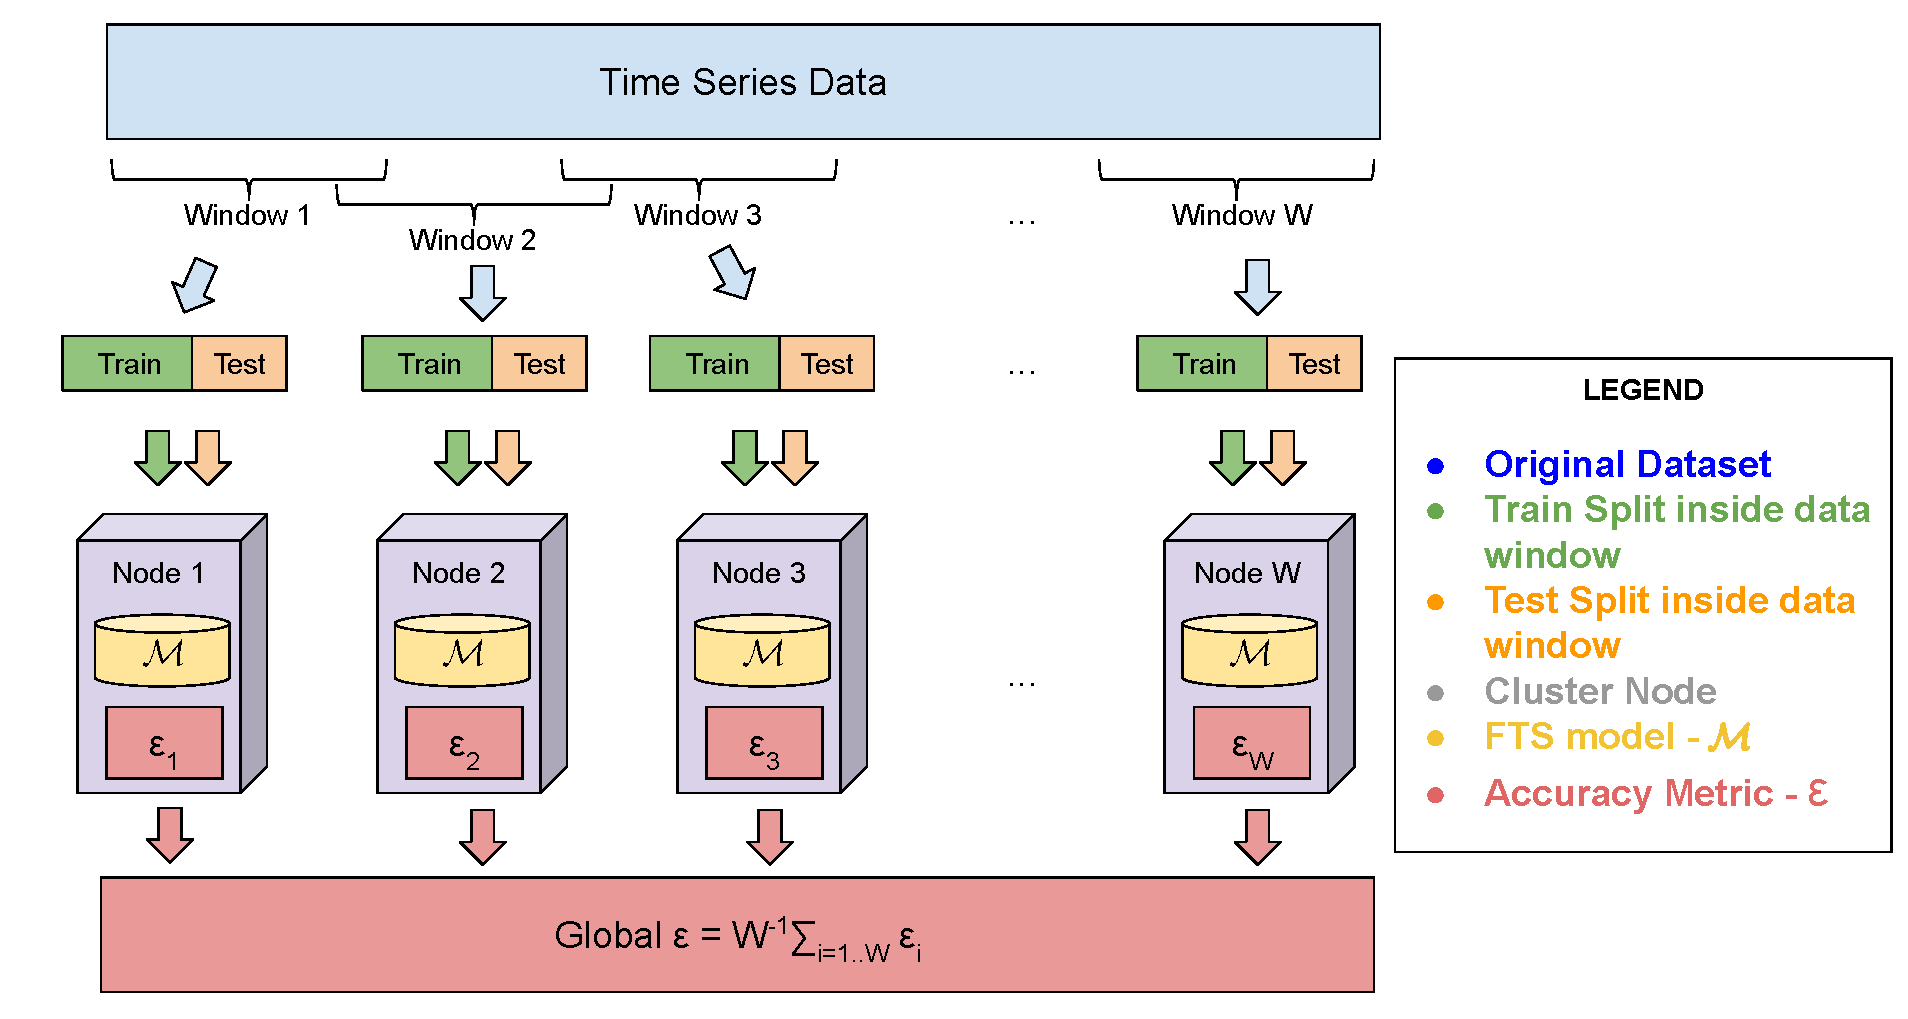
\includegraphics[width=\textwidth]{figures/distributed_testing.pdf}
    \caption{Distributed Testing With Sequential Models approach}
    \label{fig:distributed_testing}
\end{figure}

\begin{table}[htb]
    \centering
    \begin{tabular}{|c|c|p{7cm}|} \hline
        \textbf{Parameter} & \textbf{Name} & \textbf{Description} \\ \hline
         $0 < W_L < |Y|$ & Window Length & the number of time series instances in each data window \\ \hline
         $W_I \in [0,1]$ & Window Increment & Percentage of $W_L$ which is used to move the window \\ \hline
         $T_S \in [0,1]$ & Train/Test split & Percentage of $W_L$ which is used as training set and the remaining as test set.  \\ \hline
    \end{tabular}
    \caption{Distributed Testing Parameters}
    \label{tab:distributed_testing}
\end{table}

The distributed testing uses the parameters in Table \ref{tab:distributed_testing}. The number of data windows $W$ is given by $W = \max \{w\; |\; w(W_L\cdot W_I) + W_L \leq |Y| \}$ where $|Y|$ is the length of $Y$, and the process illustrated in Figure \ref{fig:distributed_testing} is executed in each evaluation of optimization engine. The key advantage of this approach is that it does not require any change on the FTS training and testing methods, just an adaption in the way the optimizer performs the evaluations. 

However, for big time series it is not enough. Depending on $|Y|$ and the capabilities of the available hardware, choosing of $W_L$ and $W_I$ may lead to three scenarios: a) $W_L$ will be larger than the available memory of the cluster nodes; b) a value of $W$ much greater than the number of cluster nodes, implicating in several rounds of computation for each node; c) $W_I$ too large that leads to the sub-sampling of the data (the windows are not overlapped and let ranges without been tested). None of these scenarios is desirable and thus a new approach must be considered.

%%%%%%%%%%%%%%%%%%%%%%%%%%%%%%%%%%%%%%%%%%%%%%%%%%%%%%%%%
%%%%%%%%%%%%%%%%%%%%%%%%%%%%%%%%%%%%%%%%%%%%%%%%%%%%%%%%%
\subsection{Distributed Models}
\label{sec:distributed_models}

For big time series the choosing of $W_L$ and $W_I$ values that do not lead to sub-sampling or cluster overhead, may fatally lead to a value of $W_L$ greater than the available machine memory. In this case even the windows must be split in smaller ones and the methodology of training and testing the models must change. Several stages of the training processes defined in Sections \ref{sec:fts_training_procedure} and  \ref{sec:pwfts_training} can be executed in parallel or distributed, on a Single Instruction/Multiple Data (SIMD) approach, since the data splits preserve the inherent time ordering. This characteristic allows the procedure's distribution to enhance their scalability and enable it to handle big time series.

This new approach changes the training method to first run the sequential procedure on individual cluster nodes with a slice of the original data window, creating a sub-model $\model_i$. Then the locally trained models are transmitted back to a master node where all local models are merged in a unique global model $\model$, as illustrated in Figure \ref{fig:distributed_models}. In the next sections the distributed training and forecasting methods are presented.

\begin{figure}[htb]
    \centering
    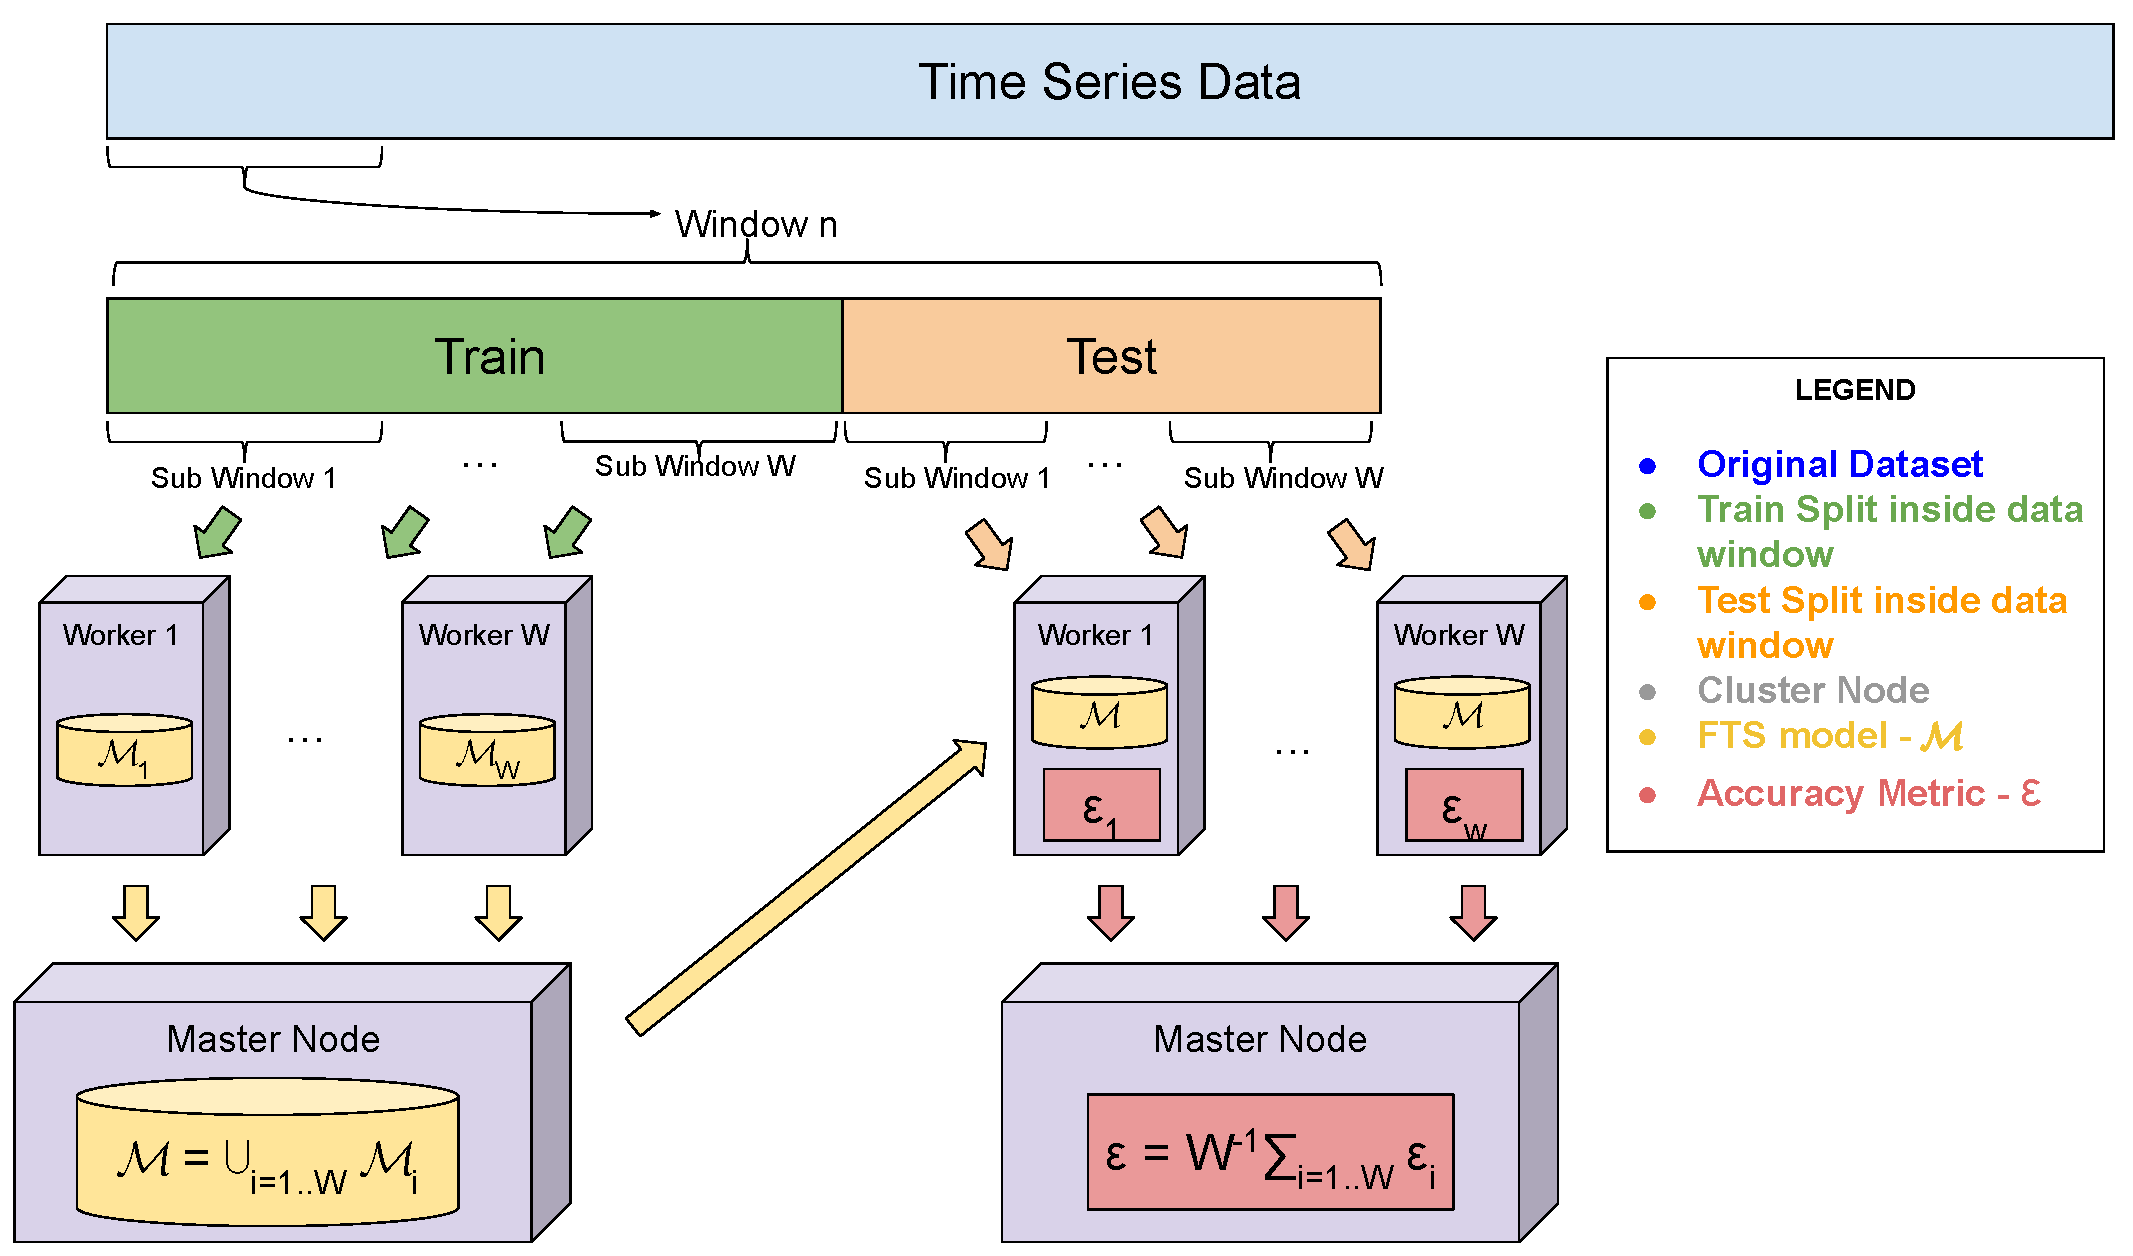
\includegraphics[width=\textwidth]{figures/distributed_models.pdf}
    \caption{Distributed Models approach}
    \label{fig:distributed_models}
\end{figure}


%%%%%%%%%%%%%%%%%%%%%%%%%%%%%%%%%%%%%%%%%%%%%%%%%%%%%%%%%
%%%%%%%%%%%%%%%%%%%%%%%%%%%%%%%%%%%%%%%%%%%%%%%%%%%%%%%%%
\subsubsection{Distributed training Procedure}
\label{sec:distributed_training}

The adaption of the sequential procedure defined in Section \ref{sec:fts_training_procedure} to the distributed one requires just few interventions. Stage 1 deeply depends on finding the universe of discourse $U$. The general procedure splits the dataset over the working nodes where the $U_i$ universes of discourse are computed. In the final step a general linguistic variable $\ulvar$, is computed by merging the locals $U_i$ as $U = \bigcup U_i$ where $\bigcup$ is the merge step.

On the other hand, the design of FTS allows the complete execution of stages 2 and 3 of training process without changes, as shown in Figure \ref{fig:distributed_models_training}. In this way, each computational node will produce its own complete model  $\mathcal{M}_i$ using its subset of the data, and on the final step a unique model  $\mathcal{M}$ is generated by merging the local models  $\mathcal{M}_i$ as  $\mathcal{M} = \bigcup \mathcal{M}_i$, where $\bigcup$ is the merge step. The complete distributed training procedure is listed below and illustrated in Figure~\ref{fig:distributed_models_training}:

\begin{enumerate}
    \item \textbf{Partitioning}:
    \begin{enumerate}
        \item \textbf{Share}: The hyperparameters $k$ and $\mu$ are shared across the cluster; 
        \item \textbf{Map}: Distribute the $Y$ dataset over the slave nodes and find $U_i$ returning it back to the master node;
        \item \textbf{Reduce}: Collect the $U_i$ from the slave nodes, mixing it on a unique interval as $U = \bigcup U_i$, where the $\bigcup$ will select the smallest lower bound and the greatest upper bound of each given interval;
        \item \textbf{Create}: Once the universe of discourse $U$ were defined, the creation of the linguistic variable $\ulvar$ is performed as the steps 2 and 3 of Stage 1 of the sequential procedure. 
    \end{enumerate}
    
    \item \textbf{Fuzzyfication \& Rule Induction}:
    \begin{enumerate}
        \item \textbf{Share}: The linguistic variable $\ulvar$ and the $\alpha$ hyperparameters are shared across the cluster;
        \item \textbf{Map}: Distribute the $Y$ dataset over the slave nodes and perform the fuzzyfication and rule induction for each subset, generating a local FTS model $\model_i$ which is returned to the master; 
        \item \textbf{Reduce}: Collect all $\model_i$ models; 
        \item \textbf{Merge}: Create an empty FTS model $\model$. For each rule $LHS \rightarrow RHS$ in all collected models $\model_i$:
        \begin{enumerate}
            \item If $\model$ does not contain the $LHS$, then append the entire rule on $\model$;
            \item If $\model$ contains the $LHS$, then for each $w_j \cdot \ufset \in RHS$:
            \begin{enumerate}
            \item If the $RHS$ on $\model$ does not contain $\ufset$, then append $w_j \cdot \ufset$ on $RHS$ and add $w_j$ on $\#RHS$
            \item If the $RHS$ on $\model$ contains $\ufset$, then add $w_j$ on existing weight and add $w_j$ on $\#RHS$
            \end{enumerate}
        \end{enumerate}
    \end{enumerate}
\end{enumerate}


\begin{figure}[htb]
    \centering
    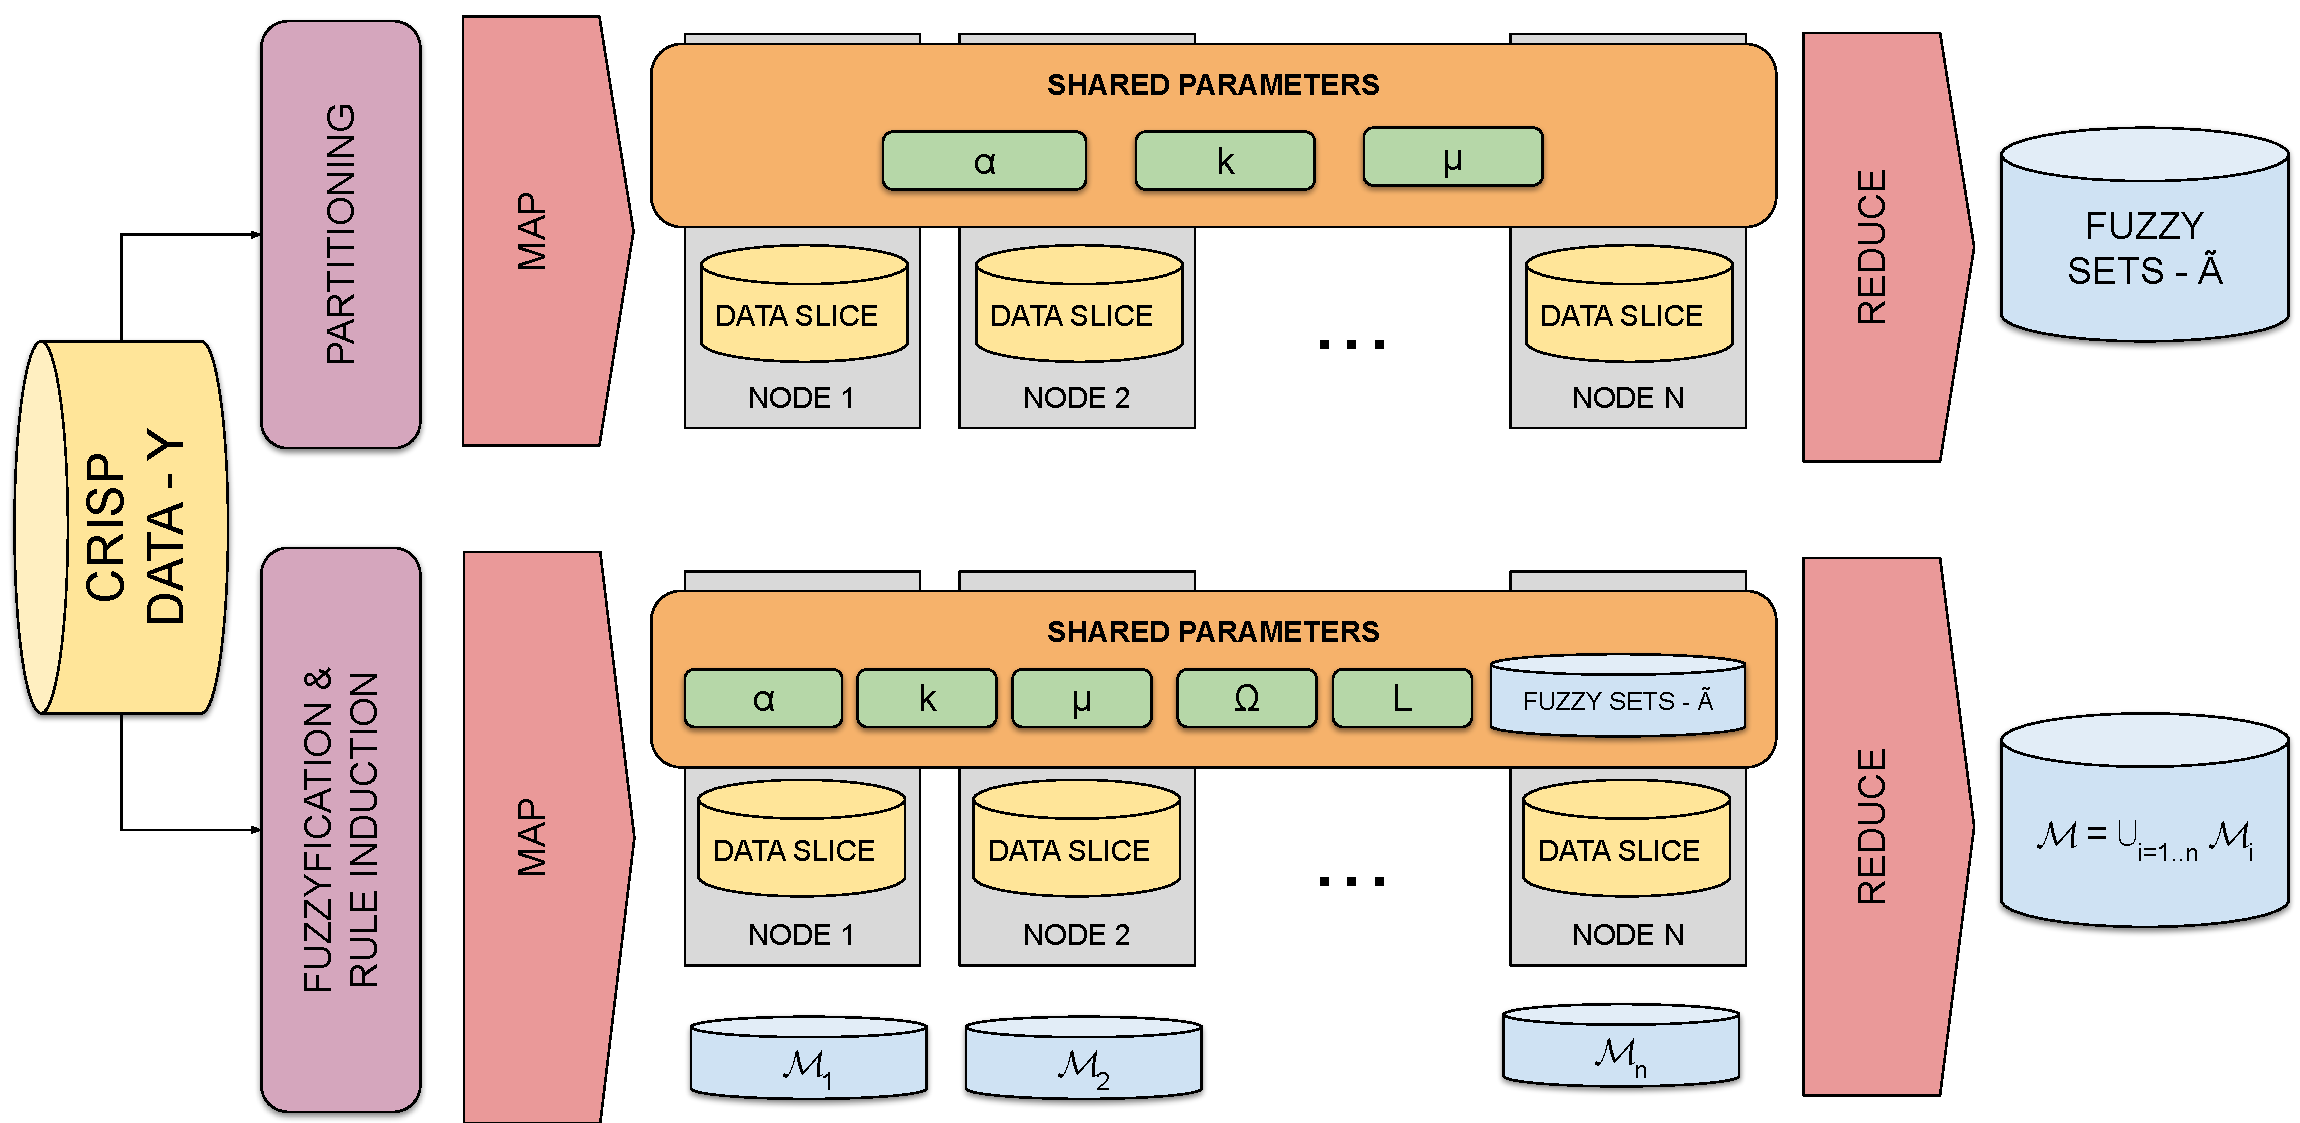
\includegraphics[width=\textwidth]{figures/distributed_models_training.pdf}
    \caption{Training of distributed models}
    \label{fig:distributed_models_training}
\end{figure}

%%%%%%%%%%%%%%%%%%%%%%%%%%%%%%%%%%%%%%%%%%%%%%%%%%%%%%%%%
%%%%%%%%%%%%%%%%%%%%%%%%%%%%%%%%%%%%%%%%%%%%%%%%%%%%%%%%%
\subsubsection{Distributed forecasting procedure}
\label{sec:distributed_forecasting}

The computational cost of the forecasting procedure is low when compared with the training procedure. The forecasting procedure bottlenecks are the fuzzyfication and rule matching steps, and both of them can be optimized using spatial indexes, for instance KD-trees \citep{Muja2014}, which are more efficient when executed locally. Also, as on every distributed procedure, the communication overhead makes this procedure inefficient for data with low volume.

However, there are occasions where the model needs to be used for forecasting in batch, where the input has high volume and one step ahead forecasting will be performed for each data point. This scenario is common in model testing, simulation and hyper-parameter optimization. In these cases it is profitable to share the parameters of the model $\mathcal{M}$ across several slave nodes and perform the forecasting on data splits, keeping its time ordering. The steps of the distributed forecasting procedure are listed below:

 \begin{enumerate}
    \item \textbf{Share}: The linguistic variable $\ulvar$ and the rules $\model$ are shared across the cluster; 
    \item \textbf{Map}: Distribute the $Y$ dataset over the slave nodes, such that each split is labelled with its time ordering;
    \item \textbf{Forecast} Each slave node receives a data split $Y_p$ and executes the sequential forecasting process, generating the estimates $\hat{Y_p}$, sending it back to the master node with the same time label received with $Y_p$;
    \item \textbf{Reduce}: Collect the $\hat{Y_p}$ estimates from the slave nodes;
    \item \textbf{Merge}: Sort the $\hat{Y_p}$ estimates by their time label and concatenate them on a unique dataset $\hat{Y}$.
\end{enumerate}


The proposed distributed methods speed up, or even make possible, to tackle high processing tasks, for instance iterative optimization procedures, using big time series and the previously proposed FTS methods. In next section an adaption of evolutionary algorithm is proposed to FTS hyperparameter optimization. 


%%%%%%%%%%%%%%%%%%%%%%%%%%%%%%%%%%%%%%%%%%%%%%%%%%%%%%%%%
%%%%%%%%%%%%%%%%%%%%%%%%%%%%%%%%%%%%%%%%%%%%%%%%%%%%%%%%%
\section{Distributed Evolutionary Hyperparameter Optimization}
\label{sec:hyperparameter}
\index{Distributed Evolutionary Hyperparameter Optimization}\index{DEHO}

This section aims to propose the Distributed Evolutionary Hyperparameter Optimization - DEHO for FTS methods. The DEHO approach combines the FTS distributed training and forecasting methods with evolutionary optimization algorithms, specifically Genetic Algorithms, in order to optimize FTS models in terms of accuracy and parsimony for big time series.

Given a set of hyperparameters $\Theta$ and an accuracy function $f: \Theta \rightarrow \mathbb{R}^+$, the hyperparameter optimization task aims to discover the values of each hyperparameter $\theta \in \Theta$ such that $\hat{\theta} = \arg\min_\theta f(\Theta)$. The hyperparameter optimization is a computational expensive task and, on a Big Data context, its cost may be prohibitive. The general FTS training procedure does not incorporate any kind of optimization, leaving to the user the task of empirically searching for the best hyperparameters. In the meantime, these parameters have great impact on final model performance and their optimization is highly recommended. At this point, it is necessary to take advantage of the speed up provided by the distributed method in Section \ref{sec:distributed} and to employ an efficient optimization method. 

It is necessary to advise that the partitioning method $\Pi$ was taken out of the optimization, and was kept constant as the Grid Partitioning. The reason is that, besides the Grid Partitioning, the other heuristic and metaheuristic $\Pi$ methods can not be trained with separated data and after merged without compromising its original features. This special aspect must be the subject of future investigations in order to enhance the DEHO method.

Two conflicting goals are sought during the hyperparameter optimization, the accuracy and the parsimony (the structural complexity as usually measured by the number of parameters of the model). In fuzzy time series models, to increase model's accuracy  it is common to increase the number of fuzzy sets $k$ and/or the order $\Omega$ of the model, which automatically increases the number of fuzzy rules $|\model|$. As the number of rules grows, the computational complexity of the model also increases and the FTS approach becomes less interesting when compared with other standard approaches, such as ARIMA or QAR. The challenge is to find a balance between these two objectives, keeping the model small, fast and accurate.

The FTS hyperparameter optimization problem is formulated below, where the objective function $f_1$ \eqref{eqn:hyperopt_f1} controls the accuracy (represented by the weighted sum of the mean error $\bar{\epsilon}$ \eqref{eqn:hyperopt_error_avg} and the standard deviation of the error $\sigma_\epsilon$ \eqref{eqn:hyperopt_error_std}) of the model and the objective function $f_2$ \eqref{eqn:hyperopt_f2} controls for parsimony (represented by the weighted sum of the model length $|\mathcal{M}|$ \eqref{eqn:hyperopt_num_rules} and the sum of the lags $|L|$ \eqref{eqn:hyperopt_lags_sum}). Some additional restrictions are imposed on the order $\Omega$ \eqref{eqn:hyperopt_order}, number of partitions $k$ \eqref{eqn:hyperopt_num_partitions}, $\alpha$-cut \eqref{eqn:hyperopt_alpha_cut}, and the lags indexes $L$ \eqref{eqn:hyperopt_lag_inc}. 

\textbf{Optimize}:
\begin{align}
minimize \quad  f_1  = & \quad 0.6\bar{\epsilon} + 0.4\sigma_\epsilon \label{eqn:hyperopt_f1}\\
minimize \quad  f_2  = & \quad 0.6|\mathcal{M}| + 0.4|L|  \label{eqn:hyperopt_f2}
\end{align}

\textbf{Where:}
\begin{equation}
RMSE = \sqrt{\sum_{t=0}^n (y(t) - \hat{y}(t))^2 )}
 \label{eqn:hyperopt_rmse}
\end{equation}
\begin{align}
\bar{\epsilon} & =  W^{-1}\sum_{i=0}^W RMSE(i) \label{eqn:hyperopt_error_avg} \\
\sigma_\epsilon & =  W^{-1}\sum_{i=0}^W \bar{\epsilon} - RMSE(i)  \label{eqn:hyperopt_error_std}
\end{align}
\begin{align}
|\model| &= \sum_{i=0}^{rules} 1  \label{eqn:hyperopt_num_rules} \\
|L| &= \sum_{i=0}^{\Omega-1} L(i)  \label{eqn:hyperopt_lags_sum} 
\end{align}

\textbf{Subject to}:

\begin{align}
\Omega &\geq 1  \label{eqn:hyperopt_order}\\
k &\geq 3  \label{eqn:hyperopt_num_partitions}\\
\alpha &\in [0,1)  \label{eqn:hyperopt_alpha_cut}\\
1 \leq L(0) & < ... < L(\Omega)  \label{eqn:hyperopt_lag_inc}
\end{align}

Genetic Algorithms (GA) are population-based metaheurisc approaches for solving the optimization problems based on a genetic refinement metaphor. Vanilla GA algorithms are intended for mono-objetive optimization, but with few adaptions it is possible to handle multi-objetive problems as well. In this work the adaptions were made on selection operator, which implements the Double Tournament strategy in order to comprise both objectives on balancing the population.

The set of hyperparameters $\Theta$ is presented in Table \ref{tab:fts_hyperparameters}, except the partitioning method $\Pi$, such that $\Theta = \{\mu,k,\alpha,\Omega,L\}$. Each individual of the population is represented by a vector - the genotype - with the values of each hyperparameter $\theta \in \Theta$. This vector contains both real, categorical and array values, according to hyperparameter type. The GA iterates over steps listed below until the stop criteria is achieved:

\begin{enumerate}
    \item \textbf{Initial Population}: The initial population, with size $NP$, is generated randomly, except for the hyperparameter $L$, whose size is constrained by $\Omega$ and the lag indexes initially consider the most significant ACF/PACF lags.
    
    \item \textbf{Evaluation:} Each genotype is transformed into a trained model - the phenotype - using the distributed method of Section \ref{sec:distributed} and then evaluated. The phenotype evaluation uses the metrics according the objective function $f_1$ and $f_2$ and after the evaluation procedure, the population is sorted by $f_1$ and $f_2$ in ascending order.

    \item \textbf{Selection:} The selection operator is responsible to choose one part of the individuals that will survive for the next generation. As the problem is multi-objective, a Double Tournament strategy was implemented to balance the selection between the two objectives. In the double tournament, the first round chooses randomly two pairs of individuals in the population, and each pair will compete with each other based on objective $f_1$. On the second round the winner individuals of the first round will compete with each other based on the objective $f_2$. This process is repeated by a rate $SR$ of the population.
    
    \item \textbf{Elitism:} As the selection operator is random, there is the possibility that the best individual of the population be discarded. The elitist strategy will keep the best individual of the current generation in the next generation and discard the worst.

    \item \textbf{Crossover:} The crossover operator combines the genotypes of two individuals ($i_1$ and $i_2$) in order to generate a descendent individual ($i_N$). On crossover, two individuals are randomly selected in the population and ordered as $i_1$ and $i_2$ according to their $f_1$ and $f_2$ objectives. For all genes the mixing process will give a major contribution for the best ranked individual (with $.7$ and $.3$ rates). For the real coded genes a linear combination as $i_N = .7i_1 + .3i_2$ will be performed. For the categorical genes, the value of $i_N$ will be $i_1$ with probability $.7$ or $i_2$ otherwise. For the lag $L$ the individual lags will be also a linear combination of each lag. This process is repeated by a rate $CR$ of the population.

    \item \textbf{Mutation:} The mutation operator aims to introduce novelties in the population, then an individual is randomly chosen and random perturbations are applied to its genes, taking care to keep the gene values feasible according to the problem restrictions. This process is repeated by a rate $MR$ of the population.

    \item \textbf{Stop Criteria:} Repeat the steps 2 to 7 until one of these criteria are achieved: $NG_{stop}$ generations without improvement or maximum number of generations $NG$.
\end{enumerate}

This Genetic Algorithm requires the choice of the  parameters presented in Table \ref{tab:genetic_algoritm}. The complete hyper-parameter optimization method also requires the choosing of the distribution type and the parameters presented in Table \ref{tab:distributed_testing}.

\begin{table}[htb]
    \centering
    \begin{tabular}{|c|p{7cm}|} \hline
        \textbf{Parameter} & \textbf{Description}  \\ \hline
         $PS \in \mathbb{N}^+$ & Population Size \\ \hline
         $NG \in \mathbb{N}^+$ & Max Number of Generations \\ \hline 
         $0 < NG_{stop} < NG$ & Max Number of Generations without improvement \\ \hline 
         $SR \in [0,1]$ & Selection Rate \\ \hline 
         $CR \in [0,1]$ & Crossover Rate \\ \hline 
         $MR \in [0,1]$ & Mutation Rate \\ \hline 
    \end{tabular}
    \caption{Genetic Algorithm parameters}
    \label{tab:genetic_algoritm}
\end{table}

%%%%%%%%%%%%%%%%%%%%%%%%%%%%%%%%%%%%%%%%%%%%%%%%%%%%%%%%%
%%%%%%%%%%%%%%%%%%%%%%%%%%%%%%%%%%%%%%%%%%%%%%%%%%%%%%%%%

\section{Computational Experiments}
\label{sec:scalability_experiments}

This section presents an exploratory study of distributed models performance and the DEHO method. The computational experiments employed a large sized environmental time series, the SONDA dataset with 2,000,000 instances, and a medium sized time series, the Malaysia dataset, with 17,000 instances. Both datasets are detailed in Appendix \ref{apd:multivariate_datasets}, where its main characteristics are presented.

In Section \ref{sec:scalability_speedup} the speed ups provided by the distributed training and forecasting are presented by several cluster configurations. In \ref{sec:scalability_convergence} the distributed methods are employed in DEHO method, and the convergence of the method is analyzed.

In order to contribute with the replication of all the results in the research, all data and source codes employed in this chapter are available at the URL:
\texttt{\url{http://bit.ly/scalable_probabilistic_fts_chap5}}

%%%%%%%%%%%%%%%%%%%%%%%%%%%%%%%%%%%%%%%%%%%%%%%%%%%%%%%%%
%%%%%%%%%%%%%%%%%%%%%%%%%%%%%%%%%%%%%%%%%%%%%%%%%%%%%%%%%
\subsection{Speed Up Of Distributed Methods}
\label{sec:scalability_speedup}

In order to assess the impact of including more processing nodes on training and forecasting processing times of distributed methods, different cluster configurations were evaluated .

The performance of the sequential and distributed methods, on above cited clusters configurations, was measured in terms of execution time (in seconds) and the speed up from the sequential time, such that $S_p = \frac{T_1}{T_p}$, where $S_p$ is the speed up for $p$ nodes, $T_1$ is the time of the sequential execution and $T_p$ is the time of the distributed execution with $p$ nodes. 

The experiments show improvements on performance for each added node on the large sized dataset, but this improvement is smaller in the medium sized dataset.  The trade-off between the distribution overhead and the benefit of the distributed computations stops to be profitable above the third node on the cluster for medium sized datasets. Above 3 nodes the network overhead for the length of data makes the distributed algorithm not interesting. However, it can be seen that an average speed up of 2x was achieved on the training procedure for large time series, showing that the performance tends to increase on more robust computational clusters.  


\begin{table}[ht]
\resizebox{\textwidth}{!}{% <------ Don't forget this %
    \centering
    \begin{tabular}{|c|c|c|c|c|c|} \hline
        Dataset & CPU's 
        & \begin{tabular}{c} Training \\ Time \end{tabular} 
        & \begin{tabular}{c} Training \\ Speed Up \end{tabular}
        & \begin{tabular}{c} Forecasting \\ Time  \end{tabular}
        & \begin{tabular}{c} Forecasting \\ Speed Up \end{tabular}  \\ \hline
        \multirow{7}{*}{SONDA Wind Speed} 
             & 1 & 685.25 $\pm$ 135.16 & - & 285.89 $\pm$ 57.94 & - \\ \cline{2-6}
             & 2 & 383.29 $\pm$ 72.50 & 1.78 & 164.82 $\pm$ 30.10 & 1.73 \\ \cline{2-6}
             & 3 & 330.13 $\pm$ 64.55 & 2.07 & 138.58 $\pm$ 25.37 & 2.06 \\ \cline{2-6}
             & 4 & 342.64 $\pm$ 52.86 & 1.99 & 151.34 $\pm$ 25.54 & 1.88 \\ \cline{2-6}
             & 5 & 300.75 $\pm$ 58.19 & 2.27 & 130.67 $\pm$ 23.20 & 2.18 \\ \cline{2-6}
             & 6 & 348.98 $\pm$ 67.41 & 1.96 & 153.16 $\pm$ 30.0 & 1.86 \\ \cline{2-6}
             & 7 & 361.45 $\pm$ 65.61 & 1.89 & 160.74 $\pm$ 30.68 & 1.77 \\ \hline
        \multirow{7}{*}{SONDA Solar Radiation }
             & 1 & 651.29 $\pm$ 121.95 & - & 274.28 $\pm$ 47.72 & - \\ \cline{2-6}
             & 2 & 383.24 $\pm$ 66.37 & 1.69 & 165.98 $\pm$ 36.21 & 1.65 \\ \cline{2-6}
             & 3 & 314.10 $\pm$ 59.98 & 2.07 & 136.92 $\pm$ 24.63 & 2.00 \\ \cline{2-6}
             & 4 & 345.55 $\pm$ 64.135 & 1.88 & 152.31 $\pm$ 28.43 & 1.8 \\ \cline{2-6}
             & 5 & 289.38 $\pm$ 54.44 & 2.25 & 129.52 $\pm$ 24.22 & 2.11 \\ \cline{2-6}
             & 6 & 340.35 $\pm$ 59.64 & 1.91 & 153.09 $\pm$ 28.35 & 1.79 \\ \cline{2-6}
             & 7 & 349.70 $\pm$ 65.48 & 1.86 & 159.16 $\pm$ 28.46 & 1.72 \\ \hline
        \multirow{7}{*}{Malaysia Temperature }
             & 1 & 12.28 $\pm$ 0.70 & - & 5.11 $\pm$ 0.35 & - \\ \cline{2-6}
             & 2 & 7.21 $\pm$ 0.48 & 1.7 & 3.42 $\pm$ 0.23 & 1.49 \\ \cline{2-6}
             & 3 & 6.64 $\pm$ 0.45 & 1.84 & 3.24 $\pm$ 0.24 & 1.57 \\ \cline{2-6}
             & 4 & 7.44 $\pm$ 0.18 & 1.64 & 3.95 $\pm$ 0.23 & 1.29 \\ \cline{2-6}
             & 5 & 6.56 $\pm$ 0.29 & 1.87 & 3.93 $\pm$ 0.47 & 1.30 \\ \cline{2-6}
             & 6 & 7.46 $\pm$ 0.24 & 1.64 & 4.44 $\pm$ 0.23 & 1.15 \\ \cline{2-6}
             & 7 & 8.09 $\pm$ 0.27 & 1.51 & 5.15 $\pm$ 0.01 & 0.99 \\ \hline
        \multirow{7}{*}{Malaysia Load }
             & 1 & 13.05 $\pm$ 1.50 & - & 5.32 $\pm$ 0.59 & - \\ \cline{2-6}
             & 2 & 7.84 $\pm$ 0.9 & 1.66 & 3.43 $\pm$ 0.24 & 1.54 \\ \cline{2-6}
             & 3 & 7.14 $\pm$ 0.75 & 1.82 & 3.42 $\pm$ 0.21 & 1.55 \\ \cline{2-6}
             & 4 & 8.06 $\pm$ 1.01 & 1.61 & 4.31 $\pm$ 0.39 & 1.23 \\ \cline{2-6}
             & 5 & 8.18 $\pm$ 2.31 & 1.59 & 4.10 $\pm$ 0.41 & 1.29 \\ \cline{2-6}
             & 6 & 8.06 $\pm$ 1.01 & 1.61 & 4.77 $\pm$ 0.46 & 1.11 \\ \cline{2-6}
             & 7 & 8.90 $\pm$ 0.86 & 1.46 & 6.18 $\pm$ 0.71 & 0.86 \\ \hline
    \end{tabular}
    }
    \caption{Speed up provided by the distributed model by number of CPU's}
    \label{tab:speed_up}
\end{table}

\begin{figure}
    \centering
    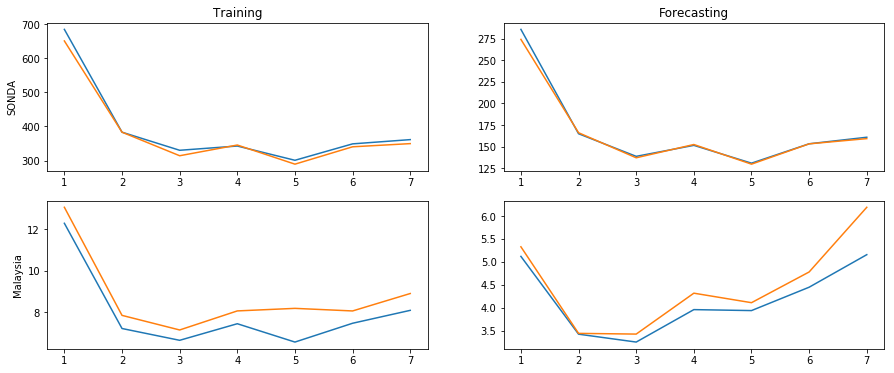
\includegraphics[width=\textwidth]{figures/speed_up.png}
    \caption{Speed up provided by the distributed model by number of CPU's}
    \label{fig:speed_up}
\end{figure}

%%%%%%%%%%%%%%%%%%%%%%%%%%%%%%%%%%%%%%%%%%%%%%%%%%%%%%%%%
%%%%%%%%%%%%%%%%%%%%%%%%%%%%%%%%%%%%%%%%%%%%%%%%%%%%%%%%%
\subsection{Convergence of DEHO approach}
\label{sec:scalability_convergence}

The DEHO method was employed using a computational cluster with 7 CPU's and the parameters contained in Table \ref{tab:hyperopt_parameters} using PWFTS as FTS method. The experiment performed 5 executions of DEHO for each dataset and the averaged results are presented in Table \ref{tab:hyperopt_results}. A sample of the convergence process of DEHO can be seen in Figure \ref{fig:deho_convergence}, for  SONDA Wind Speed dataset. 

The results showed that, for the studied time series, the convergence was fast, expending about 16 generations on average. In the trade off between the objectives $f_1$ and $f_2$, the accuracy objective showed to be predominant over the parsimony objective during the convergence of the method. 

The optimized values for the hyperparameters generated parsimonic and accurated forecasting models, whose samples of their performance can be seen in Figure

\begin{table}[htb]
    \centering
    \begin{tabular}{|c|c|c|} \hline
        \textbf{Parameter} & \textbf{Dataset} & \textbf{Value} \\ \hline
         \multirow{4}{*}{$W_L$}  & 
         \begin{tabular}{c}
              SONDA  \\
              Wind Speed 
         \end{tabular} & 600,000 \\ \cline{2-3}
                & 
        \begin{tabular}{c}
              SONDA  \\
              Solar Radiation  
         \end{tabular} & 600,000 \\ \cline{2-3}
                & 
        \begin{tabular}{c}
              Malaysia  \\
              Temperature  
         \end{tabular} & 10,000 \\ \cline{2-3}
                & 
        \begin{tabular}{c}
              Malaysia  \\
              Eletric Load  
         \end{tabular} & 10,000 \\ \hline
         $W_I$ & All &  .5 \\ \hline
         $T_S$ &  All &.9  \\ \hline
         $PS$ &  All &20  \\ \hline
         $NG$ &  All &30  \\ \hline 
         $NG_{stop}$  &  All &10  \\ \hline 
         $SR$ &  All &.5  \\ \hline 
         $CR$ &  All &.5  \\ \hline 
         $MR$ &  All &.2  \\ \hline  
    \end{tabular}
    \caption{Distributed Evolutive Hyperparameter Optimization parameter values}
    \label{tab:hyperopt_parameters}
\end{table}


\begin{table}[htb]
\resizebox{\textwidth}{!}{% <------ Don't forget this %
\begin{tabular}{|c|c|c|c|c|c|c|c|c|}
\hline
\textbf{Dataset}                       & \textbf{Generations}                                                            & $\mathbf{k}$                                                                   & $\mathbf{\mu}$     & $\mathbf{\alpha}$                                                              & $\mathbf{\Omega}$  & $\mathbf{L}$               & \textbf{Metric} & \textbf{Value}                                                  \\ \hline
\multirow{3}{*}{SONDA Solar Radiation} & \multirow{3}{*}{\begin{tabular}[c]{@{}c@{}}16.4 \\ $\pm$ 7.8\end{tabular}}      & \multirow{3}{*}{\begin{tabular}[c]{@{}c@{}}50.8 \\ $\pm$ 0.7\end{tabular}}  & \multirow{3}{*}{2} & \multirow{3}{*}{\begin{tabular}[c]{@{}c@{}}0.24 \\ $\pm$ 0.13\end{tabular}} & \multirow{3}{*}{2} & \multirow{3}{*}{{[}1,2{]}} & $|\model|$      & 613 $\pm$ 222     \\ \cline{8-9} 
                                       &                                                                                 &                                                                                &                    &                                                                                &                    &                            & RMSE            & 93.13 $\pm$ 0.62  \\ \cline{8-9} 
                                       &                                                                                 &                                                                                &                    &                                                                                &                    &                            & Time            & 3221 $\pm$ 1505   \\ \hline
\multirow{3}{*}{SONDA Wind Speed} & \multirow{3}{*}{30.0}      & \multirow{3}{*}{50}  & \multirow{3}{*}{1} & \multirow{3}{*}{\begin{tabular}[c]{@{}c@{}}0.13 \\ $\pm$ 0.1\end{tabular}} & \multirow{3}{*}{1} & \multirow{3}{*}{{[}1{]}} & $|\model|$      & 24 $\pm$ 1.45     \\ \cline{8-9} 
                                       &                                                                                 &                                                                                &                    &                                                                                &                    &                            & RMSE            & 0.34 $\pm$ 74e-10$^{-4}$  \\ \cline{8-9} 
                                       &                                                                                 &                                                                                &                    &                                                                                &                    &                            & Time            & 3058 $\pm$ 891   \\ \hline
\multirow{3}{*}{Malaysia Energy Load}  & \multirow{3}{*}{\begin{tabular}[c]{@{}c@{}}12.5 \\ $\pm$ 2.5\end{tabular}}   & \multirow{3}{*}{\begin{tabular}[c]{@{}c@{}}50.6 \\ $\pm$ 1.2\end{tabular}}  & \multirow{3}{*}{2} & \multirow{3}{*}{\begin{tabular}[c]{@{}c@{}}0.22 \\ $\pm$ 0.23\end{tabular}} & \multirow{3}{*}{2} & \multirow{3}{*}{{[}1,2{]}} & $|\model|$      & 306.9 $\pm$ 137.9 \\ \cline{8-9} 
                                       &                                                                                 &                                                                                &                    &                                                                                &                    &                            & RMSE            & 2745.5 $\pm$ 271.27                                             \\ \cline{8-9} 
                                       &                                                                                 &                                                                                &                    &                                                                                &                    &                            & Time            & 3945.09 $\pm$ 800.71                                            \\ \hline
\multirow{3}{*}{Malaysia Temperature}  & \multirow{3}{*}{\begin{tabular}[c]{@{}c@{}}16.6 \\ $\pm$ 10.15\end{tabular}} & \multirow{3}{*}{\begin{tabular}[c]{@{}c@{}}52.8 \\ $\pm$ 3.18\end{tabular}} & \multirow{3}{*}{1} & \multirow{3}{*}{\begin{tabular}[c]{@{}c@{}}0.24 \\ $\pm$ 0.09\end{tabular}} & \multirow{3}{*}{1} & \multirow{3}{*}{{[}1{]}}   & $|\model|$      & 73.21 $\pm$ 1.08                                                \\ \cline{8-9} 
                                       &                                                                                 &                                                                                &                    &                                                                                &                    &                            & RMSE            & 1.08 $\pm$ 0.06                                                 \\ \cline{8-9} 
                                       &                                                                                 &                                                                                &                    &                                                                                &                    &                            & Time            & 3916.58 $\pm$ 2042.12                                           \\ \hline
\end{tabular}
}
\caption{Optimization mean results by dataset}
\label{tab:hyperopt_results}
\end{table}

\begin{figure}[htb]
    \centering
    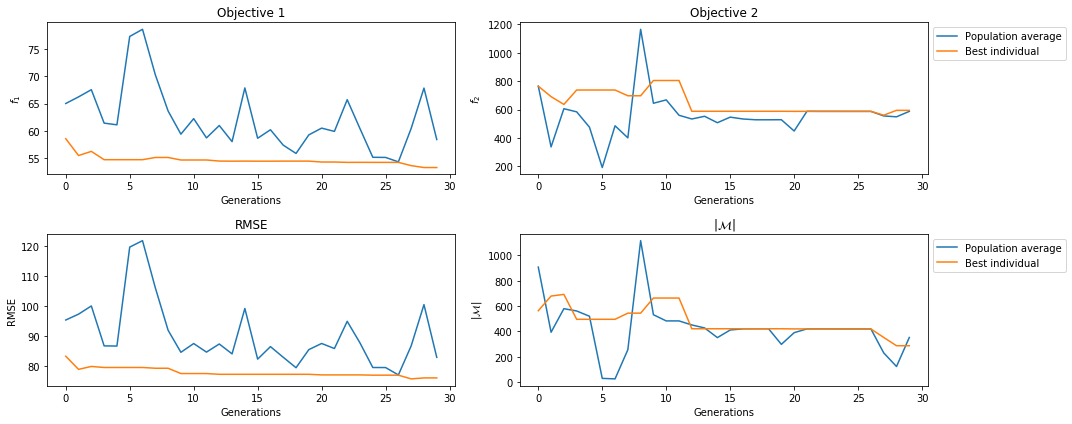
\includegraphics[width=\textwidth]{figures/deho_convergence.png}
    \caption{Sample of DEHO convergence}
    \label{fig:deho_convergence}
\end{figure}

%%%%%%%%%%%%%%%%%%%%%%%%%%%%%%%%%%%%%%%%%%%%%%%%%%%%%%%%%
%%%%%%%%%%%%%%%%%%%%%%%%%%%%%%%%%%%%%%%%%%%%%%%%%%%%%%%%%
\section{Conclusion}
\label{sec:scalability_conclusion}

Training accurate models for forecasting big time series is a challenging task for traditional and soft-computing methods. Usually the methods are not designed to deal with such high volume of data. When such data volume cannot be grounded on a single machine memory, it demands a distributed architecture of storage and processing. This is particularly problematic when optimizing the hyperparameters of a method, because successive model training and testing processes are required. 

This chapter proposed two distributed approaches for FTS model scalability, one for middle sized data and another for big sized data. The first one distributes the data across the nodes of a cluster, where individual models are trained and tested. The second one, the distributed model itself, splits the training of a unique model across several nodes, allowing a big time series model to be trained in pieces and then aggregated into a single model.

These approaches were employed on Distributed Evolutionary Hyperparameter Optimization (DEHO). DEHO method is an adapted genetic algorithm that minimizes two cost functions, the accuracy function $f_1$ and the parsimony function $f_2$. An exploratory study was performed in order to measure the feasibility of the proposed distributed models and showed the speed-up provided for big time series. The convergence of DEHO method also was analyzed, showing its effectiveness.

\subsection{Method limitations}

The distributed training method is indicated only for big time series. Using the method for small data might slow down the training time due to the network and model merging overheads. DEHO method took into account only time invariant, rule based, monovariate and high-order methods, not being applicable for time variant, multivariate and first order FTS methods.  

Next chapter presents a short review of multivariate methods and proposes a simple approach for extending PWFTS to forecasting multivariate time series.



\chapter{Multivariate Models}
\label{chap:multivariate}

Despite the existing approaches in the literature, dealing with multivariate and spatio-temporal time series was always a challenging task for FTS methods, specially because of the complexity growth of the rules as the dimension increases. An important gap in the literature is the absence of multiple input and multiple output (MIMO) methods - the majority of FTS literature consists of basically univariate forecasting methods.  

A simple approach is to transform multivariate time series into monovariate time series by using Fuzzy Information Granules (FIG). Each FIG acts as a multivariate fuzzy set, or a composition of individual fuzzy sets from different variables, allowing to replace a vector (the values of one data point) by a scalar (the identification of the FIG with the highest membership of that data point).

This approach is employed on Fuzzy Information Granular Fuzzy Time Series ($\FIG$-FTS), a wrapper method that enables PWFTS to tackle multivariate time series. It begins by partitioning the Universe of Discourse of each individual variable. Then the crisp values of each variable are fuzzyfied and the corresponding fuzzy sets are combined to create one Fuzzy Information Granule, such that it can be used as a reference of all data points in that same region. This incremental approach creates the FIGs on demand, according to the training data, and its sensibility can be controlled using the method's hyper-parameters. 

This chapter presents a short review of multivariate FTS methods and Fuzzy Information Granules on Section \ref{sec:fts_multivariate}. On Section \ref{sec:mvfts} presents a conventional method for multivariate FTS (MVFTS), which not employs FIGs. On Section \ref{sec:fig_fts} the Fuzzy Information Granule Fuzzy Time Series ($\FIG$-FTS) is proposed to enable PWFTS method be used for multivariate data and allowing the use of its interval and probabilistic forecasting features. In Section \ref{} an exploratory study of the performance of $\FIG$-FTS when compared with previous FTS methods and finally, on Section \ref{}, the results are discussed conclusions a 


%%%%%%%%%%%%%%%%%%%%%%%%%%%%%%%%%%%%%%%%%%%%%%%%%%%%%%%%%%%%%
%%%%%%%%%%%%%%%%%%%%%%%%%%%%%%%%%%%%%%%%%%%%%%%%%%%%%%%%%%%%%
\section{Multivariate FTS Methods}
\label{sec:fts_multivariate}

Multivariate time series are sets of sequential vectors of the form $Y \in \mathbb{R}^n$ where $n = |\var|$ and $\var$ is the set of attributes of $Y$. Each vector $y(t) \in Y$ contains all attributes $\vari \in \var$ and there is a temporal dependence between these data points such that their temporal ordering -- given by the time index $t \in T$ -- must be respected. 

In FTS literature it is common to employ clusterization methods to reduce multivariate data in monovariate ones, as can be seen in \cite{Li2008b}, \cite{Chen2010}, \cite{sun2014} that employs Fuzzy C-Means (FCM) clustering algorithm to create multi-variate FLRG's.

\cite{Chen2011} introduced the concept of \textit{Fuzzy Variation Groups} - FVG for bivariate FTS, where each FGP groups the FLRG's of each variable by their co-occurrence. \cite{Askari2015} proposes the \textit{High-Order Multi-Variable FTS} - HMV-FTS algorithm based on FCM clustering to generate the multi-variable FLRG's. \cite{Jilani2008} proposed the \textit{Multivariate Stochastic FTS} - MSFTS based on the exponential smoothing between the diverse variables.

\subsection{Fuzzy Information Granules}

The concept of Fuzzy Information Granules (FIG) was first proposed in \cite{Zadeh1996} as a way to define entities that represent subsets (or granules) of a wider domain. There are some works in the FTS literature where this concept is mixed with the partition of the Universe of Discourse, as discussed in \cite{Lu2014, Chen2015}, but there are several ways to define FIG in the literature. 

For univariate time series it is common to define a FIG as representative set of sub-samples of the data, so each FIG is a common temporal pattern as in \cite{Yang2017b}. The construction of this kind of FIG usually employs the clustering of sub-sequences, as in \cite{Magalhaes2008}. In \cite{Wang2014a, Wang2015} we can find a univariate fuzzy time series approach whose FIGs are a combination of unequal partitioning of the UoD and prototype sub-sequences. 

For multivariate time series FIGs are usually represented as hyper-boxes or multidimensional clusters in the feature space, as in \cite{Reyes-Galaviz2016, Singh2018}.  In \cite{Singh2018},  a multivariate fuzzy time series method is presented, which uses a bio-inspired optimization method to create FIGs by iteratively adjusting the interval lengths of each variable.

Other non-FTS granular approaches can also be found in the literature, as the Granular Functional Forecasting (GFM), proposed in \cite{Magalhaes2008}, a univariate forecasting method based on Takagi-Sugeno fuzzy system where FIGs are created using clustering methods. In \cite{Leite2011}, the authors propose the fuzzy set  based  granular  evolving modeling (FBeM) approach for time series prediction, later extended in \cite{Soares2018} for spatio-temporal data.

There are some notable drawbacks in the previous methods, namely: a) the absence of multivariate forecast (MIMO); b) the use of optimization methods to create the FIGs, which makes the learning process computationally expensive; c)~the absence of multivariate FTS methods that could provide both weighted and high order characteristics. To fix these drawbacks this work proposes the $\mathcal{FIG}$-FTS method, a weighted and high-order FTS method that will be discussed in the next sections. 

%%%%%%%%%%%%%%%%%%%%%%%%%%%%%%%%%%%%%%%%%%%%%%%%%%%%%%%%%
%%%%%%%%%%%%%%%%%%%%%%%%%%%%%%%%%%%%%%%%%%%%%%%%%%%%%%%%%
\section{The Conventional Multivariate Fuzzy Time Series method}
\label{sec:mvfts}

Just as it was done in Chapter \ref{chap:review_fts}, this section propose a consensus model for rule based multivariate FTS that extends the model of \cite{chen1996forecasting} to the multivariate case. The Conventional Multivariate Fuzzy Time Series (MVFTS) method was designed to allow several models to be trained individually with subsets of a greater dataset and later to be merged into a single model, feature that enhances the performance of model creation by enabling its distribution.

For each chosen variable $\vari \in \var$ on $Y$, MVFTS also incorporates several features present in the literature, represented by the hyperparameters on Table~\ref{tab:mvfts_hyperparameters}, giving versatility and flexibility to the model. The method is composed of two procedures: the training procedure and the forecasting procedure.

\begin{table}[]
    \centering
    \begin{tabular}{|c|m{2cm}|c|m{.5\textwidth}|} \hline
        \textbf{Alias} & \textbf{Parameter} & \textbf{Type} & \textbf{Description}  \\ \hline
         $k_i$ & Number of partitions & $\mathbb{N}^+$ & The number of fuzzy sets that will be created in the linguistic variable $\mlvar$  \\ \hline
         $\mu$ & Membership function & $\mu: U \rightarrow [0,1] $ & A function that measure the membership of a value $y \in U$ to a fuzzy set  \\\hline
         $\alpha$ & $\alpha$-cut & $[0,1]$ & The minimal membership grade to take account on fuzzyfication process \\ \hline
    \end{tabular}
    \caption{WMVFTS hyperparameters for each variable $\vari \in \var$}
    \label{tab:mvfts_hyperparameters}
\end{table}

The MVFTS is a first order point forecaster of type Multiple Input/Single Output (MISO), then for the set of variables $\var$ one of them is chosen as the target (or endogenous) variable and the others are referred as the explanatory (or exogenous) variables. From now on, the target variable will be distinguished from the others by an asterisk, as $*\var$.

The training procedure, explained in subsection \ref{sec:mvfts_training_procedure} and illustrated in Figure~\ref{fig:mvfts_training_procedure}, is a three stage process responsible to create a multivariate weighted FTS model $\model$. The final MVFTS model  $\model$ consists of a set of variables $\var$, a fuzzy linguistic variable $\mlvar$ for each $\vari \in \var$ and a set of weighted fuzzy rules over the linguistic variables $\mlvar$. The inputs of the training procedure are the crisp time series training data $Y$ and the set of hyperparameters for each $\vari \in \var$.

The forecasting procedure, explained in subsection \ref{sec:mvfts_forecasting_procedure} and illustrated in Figure~\ref{fig:mvfts_forecasting_procedure}, aims to produce a point estimate $\estimate$ for the target variable $*\var$, given an input sample $Y$, using the linguistic variables $\mlvar$ and the induced fuzzy rules on model $\model$.

%%%%%%%%%%%%%%%%%%%%%%%%%%%%%%%%%%%%%%%%%%%%%%%%%%%%%%%%%
%%%%%%%%%%%%%%%%%%%%%%%%%%%%%%%%%%%%%%%%%%%%%%%%%%%%%%%%%
\subsection{Training Procedure}
\label{sec:mvfts_training_procedure}

\begin{figure}
\centering
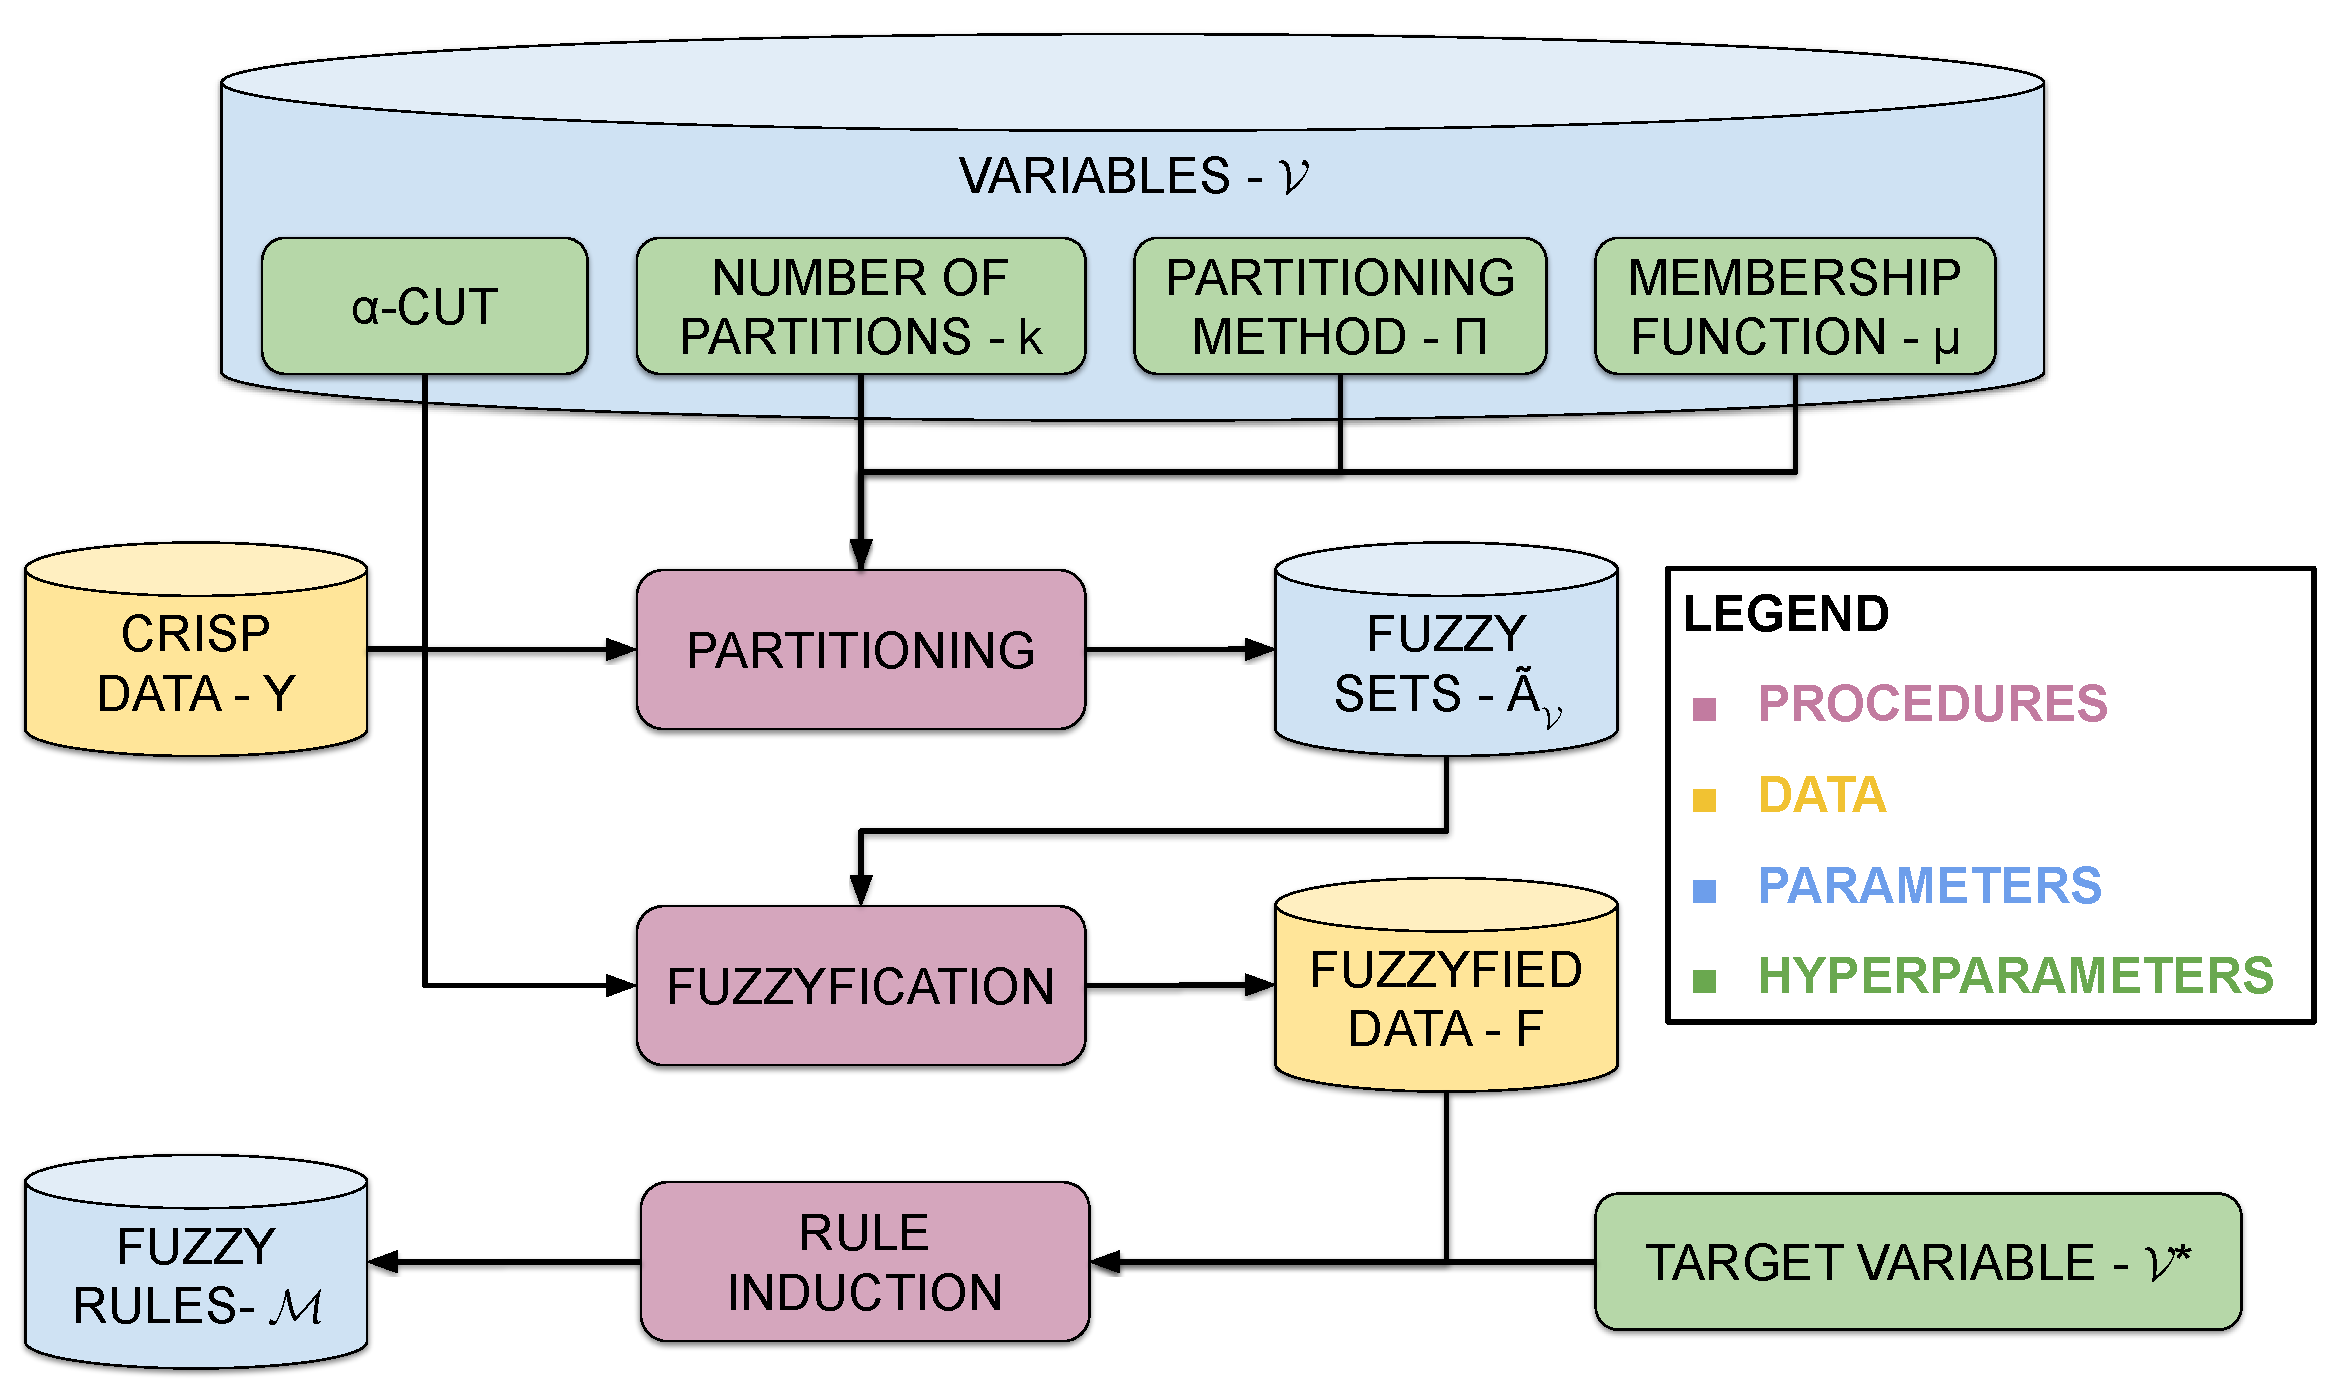
\includegraphics[width=\textwidth]{figures/mvfts_training_procedure.pdf}
\caption{MVFTS training procedure} \label{fig:mvfts_training_procedure}
\end{figure}

\begin{enumerate}
\item[Stage 1] \textit{Partitioning}:
\begin{enumerate}
\item \textit{Defining $U_{\vari}$}: The Universe of Discourse $U_{\vari}$ defines the sample space, i.e., the known bounds of the variable $\vari$, such that $U_{\vari} = [\min(Y^{\vari})-D_1, \max(Y^{\vari})+D_2]$, where $D_1 = \min(Y^{\vari})\times 0.2$ and $D_2 = \max(Y^{\vari})\times 0.2$ are used to extrapolate the known bounds as a security margin, $\forall \vari \in \var$.

\item \textit{$U_{\vari}$ Partitioning}: Split $U_{\vari}$ in $k_i$ intervals $U_j$ with midpoints $c_j$, for $j=0..k_i$, where all the intervals have the same length;

\item \textit{Define the linguistic variable $\mlvar$}: For each interval $U_j \in U_{\vari}$  create an overlapping fuzzy set $\mfset$, with the membership function $\mu_{\mfset}$. The midpoint of the fuzzy set $\mfset$ will be $c_j$, the lower bound $l_j = c_{j-1}$ and the upper bound $u_j = c_{j+1}$ $\forall$ $j >0$ and $j < k_i$, and $l_0 = \min U_{\vari}$, $l_k = \max U_{\vari}$. Each fuzzy set $\mfset$ is a linguistic term of the linguistic variable $\mlvar$;
\end{enumerate}

\item[Stage 2] \textit{Fuzzyfication}: 

Transform the original numeric time series $Y$ into a fuzzy time series $F$, where each data point $f(t) \in F$ is an $n \times k$ array with the fuzzyfied values of $y(t) \in Y$ with respect to the linguistic terms $\mfset \in \mlvar$, where the fuzzy membership is greater than the predefined $\alpha$-cut, i.e., $f(t) = \{\mfset\; |\; \mu_{\mfset}(y(t)^{\vari}) \geq \alpha_i\;\forall \mfset \in \mlvar\}$;

\item[Stage 3] \textit{Rule Induction}: 
\begin{enumerate}
\item \textit{Generate the temporal patterns}: The fuzzy temporal patterns associate the fuzzyfied values $\var$ to a set of possible values of the target variable $*\var$, such that $\var \rightarrow *\var$, whith the format $A_j^{\var_0},...,A_j^{\var_n} \rightarrow A_j^{*\var}$, where the precedent, or left hand side (LHS), is $f(t - 1) = \mfset, \forall \vari \in \var$, and the consequent, or right hand side (RHS), is $f(t+1) = \tfset$, $\tfset \in \tlvar$.

\item \textit{Generate the rule base}: Select all temporal patterns with the same precedent and group their consequent sets  creating a rule with the format $\var \rightarrow w_k \cdot A_k^{*\var}, w_j \cdot A_j^{*\var},...$, where the LHS is $f(t - 1) = \mfset, \forall \vari \in \var$ and the RHS is $f(t+1) \in \{A_k^{*\var},A_j^{*\var},... \}$. Each rule can be understood as the weighted set of possibilities which may happen on time $t+1$ (the consequent) when a certain precedent $A_{i0},...,A_{i\Omega}$ is identified on previous lag (the precedent).
\end{enumerate}
\end{enumerate}


%%%%%%%%%%%%%%%%%%%%%%%%%%%%%%%%%%%%%%%%%%%%%%%%%%%%%%%%%
%%%%%%%%%%%%%%%%%%%%%%%%%%%%%%%%%%%%%%%%%%%%%%%%%%%%%%%%%
\subsection{Forecasting Procedure} 
\label{sec:mvfts_forecasting_procedure}

\begin{figure}
\centering
\includegraphics[width=\textwidth]{figures/mvfts_forecasting_procedure.pdf}
\caption{MVFTS forecasting procedure} \label{fig:mvfts_forecasting_procedure}
\end{figure}

\begin{enumerate}
\item [Step 1] \textit{Fuzzyfication}: Compute the membership grade $\mu_{ji}$ for $y(t-1) \in Y$ such that $\mu_{ji} = \mu_{\mfset}(y(t-1))$, for each $\mfset \in \mlvar$, for each $\vari \in \var$ ;
\item [Step 2] \textit{Rule matching}: Select the $K$ rules where all fuzzy sets $\mfset$ on the LHS, for each $\vari \in \var$, have $\mu_{ji} > \alpha_i$; The rule fuzzy membership grade is shown below, using the minimum function as T-norm.
\begin{equation}
    \mu_q = \bigcap_{j \in \mlvar\; ; \; i \in \var} \mu_{ji}
\end{equation}
\item [Step 3] \textit{Rule mean points}: For each selected rule $q$, compute the mean point $mp_q$ of the target variable $*\var$ as below, where $c_j$ is the $c$ parameter of the $\mu$ function from fuzzy set $\tfset$:
\begin{equation}
mp_q = \sum_{j \in *\mlvar} c_j
\end{equation}
\item [Step 4] \textit{Defuzzyfication}: Compute the forecast as the weighted sum of the rule mid-points $mp_q$ by their membership grades $\mu_q$ for each selected rule $j$:
\begin{equation}
\estimate = \frac{\sum_{q \in K} \mu_q \cdot mp_q}{\sum_{q \in K} \mu_q}
\end{equation}
\end{enumerate}

%%%%%%%%%%%%%%%%%%%%%%%%%%%%%%%%%%%%%%%%%%%%%%%%%%%%%%%%%
%%%%%%%%%%%%%%%%%%%%%%%%%%%%%%%%%%%%%%%%%%%%%%%%%%%%%%%%%
\subsection{Interval forecasting for MVFTS}
\label{sec:mvfts_interval}

The MVFTS model can be used for interval forecasting following the same approach of $\ifts$ method. For this it is needed to change the Steps 3 and 4 of the forecasting procedure presented in Section \ref{sec:mvfts_forecasting_procedure}, as presented below:

\begin{enumerate}
\item [Step 3] \textit{Rule intervals}: For each selected rule $q$, compute the interval $\intvl^q$ of the target variable $*\var$ as below, where $\underline{\tfset}$ and $\overline{\tfset}$ are respectively the lower and upper bounds of the target fuzzy sets  $\tfset$:
\begin{align}
    \intvl^q & =  [\underline{\intvl^q_{min}}, \overline{\intvl^q_{max}}] \\
    \underline{\intvl^q_{min}} &= \min(\underline{\tfset} \in *\mlvar) \\
    \overline{\intvl^q_{max}} &= \max(\overline{\tfset} \in *\mlvar) \\
\end{align}

\item [Step 4] \textit{Defuzzyfication}: Compute the prediction interval as the extrema of the rule intervals $\intvl_q$ by their membership grades $\mu_q$ for each selected rule $j$:
\begin{equation}
\mathbb{I}(t+1) = \frac{\sum_{j \in *\mlvar} \mu_q \mathbb{I}^q}{\sum_{q \in \var} \mu_q} = \frac{\sum_{q \in \var} [\mu_q\underline{\intvl^q_{min}} , \mu_q\overline{\mathbb{I}^q_{max}}] }{\sum_{q \in \var} \mu_q}
\label{eqn:mvifts}
\end{equation}
\end{enumerate}

%%%%%%%%%%%%%%%%%%%%%%%%%%%%%%%%%%%%%%%%%%%%%%%%%%%%%%%%%
%%%%%%%%%%%%%%%%%%%%%%%%%%%%%%%%%%%%%%%%%%%%%%%%%%%%%%%%%
\subsection{Weighted Multivariate FTS - WMVFTS}
\label{sec:wmvfts}

A simple extension of MVFTS to embody weights in its rules can be achieved by changing Stage 3.b of the training procedure presented on Section \ref{sec:mvfts_training_procedure}, where the new step is:

\begin{enumerate}
    \item[Stage 3.b)] \textit{Generate the rule base}: Select all temporal patterns with the same precedent and group their consequent sets  creating a rule with the format $\var \rightarrow w_k \cdot A_k^{*\var}, w_j \cdot A_j^{*\var},...$, where the LHS is $f(t - 1) = \mfset, \forall \vari \in \var$ and the RHS is $f(t+1) \in \{A_k^{*\var},A_j^{*\var},... \}$ and the weights $w_j, w_k, ...$ are the normalized frequencies of each temporal pattern such that:
\begin{equation}
w_i = \frac{\#\tfset}{\#RHS} \quad \forall \tfset \in RHS    
\end{equation}
where $\#A_i$ is the number of occurrences of $A_i$ on temporal patterns with the same precedent $LHS$ and $\#RHS$ is the total number of temporal patterns with the same precedent $LHS$.
\end{enumerate}

It is also need to change the Step 3 of the forecasting procedure presented in Section \ref{sec:mvfts_forecasting_procedure}, as presented below:

\begin{enumerate}
    \item [Step 3] \textit{Rule mean points}: For each selected rule $q$, compute the mean point $mp_q$ of the target variable $*\var$ as below, where $c_j$ is the $c$ parameter of the $\mu$ function from fuzzy set $\tfset$:
\begin{equation}
mp_q = \sum_{j \in *\mlvar} w_j \cdot c_j
\end{equation}
\end{enumerate}

For the interval forecasting method proposed in Section \ref{sec:mvfts_interval}, a new approach is adopted to create the fuzzy rule intervals, as presented below:

\begin{align}
    \intvl^q & =  [\underline{\intvl^q_{min}}, \overline{\intvl^q_{max}}] \\
    \underline{\intvl^q_{min}} &= \sum_{j \in *\mlvar} w_j \cdot \underline{\tfset} \\
    \overline{\intvl^q_{max}} &= \sum_{j \in *\mlvar} w_j \cdot \overline{\tfset} 
\end{align}

MVFTS and WMVFTS methods take separated partitionings for each variable and its rules contains references for the different variables.  In next section a simple approach is proposed for transforming multivariate time series in monovariate ones, allowing the use of monovariate FTS methods to tackle multivariate time series.

%%%%%%%%%%%%%%%%%%%%%%%%%%%%%%%%%%%%%%%%%%%%%%%%%%%%%%%%%%%%%
%%%%%%%%%%%%%%%%%%%%%%%%%%%%%%%%%%%%%%%%%%%%%%%%%%%%%%%%%%%%%
\section{Fuzzy Information Granule Fuzzy Time Series  $\FIG$-FTS}
\label{sec:fig_fts}
\index{Fuzzy Information Granules}\index{FIG-FTS}

The Fuzzy Information Granule Fuzzy Time Series ($\FIG$-FTS) is a wrapper model which enables a monovariate model (PWFTS) to tackle multivariate time series. Beyond extend PWFTS features for multivariate data, the $\mathcal{FIG}$-FTS also appends the multivariate forecasting capability, acting as a Multiple Input/Multiple Output (MIMO) method, where all variables are both targets and explanatory variables. 

The aim of $\FIG$-FTS is to replace the Partitioning and Fuzzyfication stages of the PWFTS training procedure detailed in Section \ref{sec:pwfts_training}, the Fuzzyfication step of the forecasting procedure detailed in Section \ref{sec:pwfts_forecasting} and appends the multivariate forecasting to the extensions presented in Section \ref{sec:pwfts_extensions}.

Given an $n$-variate time series $Y=(y_1(t), \ldots,y_n(t)),  t=0\ldots,T$, corresponding variables $\var_i$ are defined for each $y_i(t)$. The resulting fuzzy time series $F$ is then composed by data points $f(t) \in F$ that represent a sequence of fuzzy information granules $\figi$. Each granule contains a set of fuzzy linguistic variables $\mlvar$ related to each variable $\var_i$.

The training procedure, described in subection \ref{sec:fig_training_procedure} and illustrated on Figure \ref{fig:figfts_training_procedure}, performs the multivariate partitioning, fuzzyfication and then feeds PWFTS with the fuzzyfied data, whose is responsible for rule induction. The final $\FIG$-FTS model $\model$ consists of a set of variables $\var$, a fuzzy linguistic variable $\mlvar$ for each $\vari \in \var$, a fuzzy information granule set $\FIG$ and a set of probabilistic weighted high order fuzzy rules over the information granules $\figi \in \fig$. The training procedure employ the hyper-parameters listed on Table~\ref{tab:fig_hyperparameters}

In the training method the partitioning of each variable is independent from the others. Each variable has its own linguistic variable $\mlvar$. For this it is necessary to inform, for each chosen variable $\vari \in \var$ on $Y$, the hyper-parameters $k_i, \mu$ and $\alpha$. The order of the model is controlled by the parameter $\Omega$ and the lag indexes are controlled by the parameter $L$. 

\begin{table}[]
    \centering
    \begin{tabular}{|c|m{2cm}|c|m{.5\textwidth}|} \hline
        \textbf{Alias} & \textbf{Parameter} & \textbf{Type} & \textbf{Description}  \\ \hline
         $k_i$ & Number of partitions & $\mathbb{N}^+$ & The number of fuzzy sets that will be created in the linguistic variable $\mlvar$  \\ \hline
         $\mu$ & Membership function & $\mu: U \rightarrow [0,1] $ & A function that measure the membership of a value $y \in U$ to a fuzzy set  \\\hline
         $\alpha$ & $\alpha$-cut & $[0,1]$ & The minimal membership grade to take account on fuzzyfication process \\ \hline
         $\Omega$ & Order & $\mathbb{N}^+$ & The number of past lags used in the precedent of each fuzzy rule \\\hline
         $L$ & Lags & & A vector of the past lag indexes, with length $\Omega$ and $1 \leq L[i] < L[i+1]$ for  $t=0..\Omega$ \\ \hline
         $\kappa$ & k-nearest neighbors & $\mathbb{N}^+$ & The number of nearest neighbors that the spatial index search on $\FIG$ during the fuzzyfication process \\ \hline
    \end{tabular}
    \caption{$\mathcal{FIG}$-FTS hyper-parameters}
    \label{tab:fig_hyperparameters}
\end{table}

The global linguistic variable $\FIG$ is the union of all Fuzzy Information Granules $\figi$, which in turn are the combination of one fuzzy set for each variable, such that $\figi = \{ \mfset \}, \forall \vari \in \var$ and its membership function is given by $\mu_{\figi} = \bigcap \mu_{\mfset}$, where $\bigcap$ is the minimum T-norm. The $\FIG$ set is indexed by the midpoints of its internal fuzzy sets, enabling optimized spatial search using KD-trees.  
With the linguistic variable $\FIG$ the fuzzyfication process transforms each multivariate data point $y(t) \in Y$ into a  $\figi \in \FIG$, such that $f(t) = \figi$.

The forecasting procedure, explained in subsection \ref{sec:fig_forecasting_procedure} and illustrated on Figure \ref{fig:figfts_forecasting_procedure}, aims to produce a point estimate $\estimate$ for each variable $\var$, given an input sample $Y$, using the linguistic variable $\FIG$ and the induced fuzzy rules on model $\model$.

The rule matching procedure can become computationally expensive as the size of the rule base $\model$ grows. Because of this it is advisable that implementations of this model use spatial trees  \cite{Muja2014} to index the rules with the midpoints of each fuzzy set on their $LHS$, optimizing the search for applicable rules during the forecasting step. This work used the KD-tree implementation of the Scipy Spatial package\footnote{\url{https://docs.scipy.org/doc/scipy/reference/spatial.html}. Access in 2019-04-29.}.

The global parameter $\kappa$ is related with the spatial index search on $\FIG$, and indicates how many $\figi \in \FIG$ are returned for a given crisp multivariate data point. This parameter has influence on the sensibility and the diversity of the rules considered during the forecasting procedure, such that as $\kappa$ increases more rules will be accounted on. If $\kappa = 1$, just the closest rule (the rule with the highest membership degree) will be used. 

%%%%%%%%%%%%%%%%%%%%%%%%%%%%%%%%%%%%%%%%%%%%%%%%%%%%%%%%%
%%%%%%%%%%%%%%%%%%%%%%%%%%%%%%%%%%%%%%%%%%%%%%%%%%%%%%%%%
\subsection{Training Procedure}
\label{sec:fig_training_procedure}

\begin{figure}
\centering
\includegraphics[width=\textwidth]{figures/figfts_training_procedure.pdf}
\caption{$\mathcal{FIG}$-FTS training procedure} 
\label{fig:figfts_training_procedure}
\end{figure}

\begin{enumerate}
\item[Stage 1] \textit{Partitioning}:
\begin{enumerate}
\item \textit{Defining $U_{\vari}$}: The Universe of Discourse $U_{\vari}$ defines the sample space, i.e., the known bounds of the variable $\vari$, such that $U_{\vari} = [\min(Y^{\vari})-D_1, \max(Y^{\vari})+D_2]$, where $D_1 = \min(Y^{\vari})\times 0.2$ and $D_2 = \max(Y^{\vari})\times 0.2$ are used to extrapolate the known bounds as a security margin, $\forall \vari \in \var$.

\item \textit{$U_{\vari}$ Partitioning}: Split $U_{\vari}$ in $k_i$ intervals $U_j$ with midpoints $c_j$, for $j=0..k_i$, where all the intervals have the same length;

\item \textit{Define the linguistic variable $\mlvar$}: For each interval $U_j \in U_{\vari}$  create an overlapping fuzzy set $\mfset$, with the membership function $\mu_{\mfset}(y_{\vari}(t))$, where $y_{\vari}(t)$ is the value of the $\vari$ variable on instance $y(t) \in Y$. The midpoint of the fuzzy set $\mfset$ will be $c_j$, the lower bound $l_j = c_{j-1}$ and the upper bound $u_j = c_{j+1}$ $\forall$ $j >0$ and $j < k_i$, and $l_0 = \min U_{\vari}$, $l_k = \max U_{\vari}$. Each fuzzy set $\mfset$ is a linguistic term of the linguistic variable $\mlvar$;

\end{enumerate}

\item[Stage 2] \textit{Fuzzyfication}: 

Transform the original numeric time series $Y$ into a fuzzy time series $F$, where each data point $f(t) \in F$ is a $\fig_i \in \FIG$. For each $y(t) \in Y$ the following steps must be executed:

\begin{enumerate}
    \item \textit{Individual variable fuzzyfication}: For each variable $\vari \in \var$, find the linguistic terms $\mfset \in \mlvar$, where the fuzzy membership is greater than the predefined $\alpha$-cut, i.e., $f_{\vari}(t) = \{\mfset\; |\; \mu_{\mfset}(y_{\vari}(t)) \geq \alpha_i\;\forall \mfset \in \mlvar\}$;
    
    \item \textit{Search in $\FIG$}: For each combination of fuzzy sets $\mfset$ in $f_{\vari}(t)$ verify if there is a $\figi \in \fig$ where $\figi \supset \{ \mfset \}, \forall \mfset \in f_{\vari}(t)$. If it exists, then the fuzzyfied value of $y(t)$ is $\figi$. This search is performed with KD-trees, comparing the midpoints of the fuzzyfied data and the midpoints of the fuzzy sets in the $\FIG$.
    
    \item \textit{Create new $\figi$ in $\FIG$}: If no $\figi$ was found in the previous step, new ones are added to $\FIG$. For each combination of fuzzy sets $\mfset$ in $f_{\vari}(t)$ create a fuzzy information granule $\figi$ such that $\figi = \{ \mfset \}, \forall \mfset \in f_{\vari}(t)$ and $\mu_{\fig_i} = \bigcap \mu_{\mfset}$. The created $\figi$ is then the fuzzyfied value of $y(t)$.
\end{enumerate}


\item[Stage 3] \textit{Rule Induction}: 
\begin{enumerate}
\item The fuzzyfied data $F$ where $f(t) = [(\fig_0,\mu_{\fig_0}),\ldots,(\figi,\mu_{\figi})]$ is passed to the Rule Induction stage of PWFTS method, which create the PWFTPG model $\model$. Each high-order PWFTG rule now will have the format $\pi_j \fig_{i0},...,\fig_{i\Omega} \rightarrow w_{j0} \cdot \fig_{i0}, \ldots w_{ji} \cdot \fig_{ji}$, where the LHS is $f(t - L(\Omega)) = \fig_{i0}$, $f(t - L(\Omega-1)) = \fig_{i1}$, ..., $f(t - L(0)) = \fig_{i\Omega}$ and the RHS is $f(t+1) \in \{\fig_k, \fig_j,...\}$ and the weights $\pi_j, w_{jk}$ are the fuzzy empirical probabilities.
\end{enumerate}
\end{enumerate}


%%%%%%%%%%%%%%%%%%%%%%%%%%%%%%%%%%%%%%%%%%%%%%%%%%%%%%%%%
%%%%%%%%%%%%%%%%%%%%%%%%%%%%%%%%%%%%%%%%%%%%%%%%%%%%%%%%%
\subsection{Forecasting Procedure} 
\label{sec:fig_forecasting_procedure}

\begin{figure}
\centering
\includegraphics[width=\textwidth]{figures/figfts_forecasting_procedure.pdf}
\caption{$\mathcal{FIG}$-FTS forecasting procedure} 
\label{fig:figfts_forecasting_procedure}
\end{figure}

\begin{enumerate}
\item [Step 1] \textit{Fuzzyfication}: Find the $\kappa$ closest   $\fig_{i\Omega},...,\fig_{i0} \in \FIG$ to the input sample $y(t-\Omega),...,y(t)$. 

\item [Step 2] \textit{Rule matching}: The fuzzyfied input sample is transfered to PWFTS that search for the applicable rules. For each PWFTPG rule $j$ found, its fuzzy membership is given by:
\begin{equation}
    \mu_j = \bigcap_{t\in L\; i \in \FIG} \mu_{\fig_{it}}
\end{equation}

\item [Step 3] \textit{Defuzzyfication}: 
\begin{enumerate}
    \item \textit{Target variable selection}: For non multivariate forecasts a target variable $*\var$ must be chosen between the variables $\var$.
    \item \textit{PWFTPG adaption}: After the target variable $*\var$ be selected, the RHS of all PWFTPG's are modified, replacing the $figi$ by the fuzzy sets $\tfset \in *\mlvar$, keeping the weights untouched;
    \item \textit{Deffuzyfication}: The PWFTS deffuzyfication methods (point, interval and probabilistic) can be invoked without modifications;
\end{enumerate}

\item [Step 4] \textit{Multivariate forecasting}:
\begin{enumerate}
    \item If a target variable was not specified, compute a point forecast $\hat{y}^{\vari}(t+1)$ invoking the PWFTS point forecasting by taking each variable $\vari \in \var$ as a target variable;
    \item Merge the individual variable forecastings to create the multivariate forecast $\hat{y}(t+1) = \bigcup_{\vari \in \var} \hat{y}^{\vari}(t+1)$ 
\end{enumerate}
 
\item [Step 5] \textit{Forecasting horizon}: Given the number $m$ of steps ahead to forecast  (the forecast horizon), repeat the Steps 1 to 4 $m$ times, appending the output $\hat{y}$ of the previous Step 4 at the end of the $y(t)$ input for the next Step 1.
\end{enumerate}

\subsection{Method discussion}
\label{sec:fig_discussion}

The main insight of the $\mathcal{FIG}$-FTS is that the linguistic variables $\mlvar$ work as feature extraction layers and each fuzzy information granule $\fig$ is a small cluster prototype of these features, simplifying the representation of temporal patterns and aiding pattern identification and rule induction. Each $\fig$ also helps the multivariate defuzzyfication process, working as a final output layer for the model.

The learning procedure of $\FIG$-FTS is controlled by its hyper-parameters that directly affect its accuracy and parsimony. The number of partitions of each variable $k_i$ affects the number of rules directly, given the maximum number of rules (in the worst case) is a Cartesian product of the fuzzy sets $\mfset \in \mlvar$, for each $\vari \in \var$. The $\alpha_i$-cut, on the other hand, controls the fuzzyfication sensibility by eliminating, in  the rule induction stage, values with lower membership grades. It reduces the number of rules by preventing the capture of spurious patterns, generated by insignificant memberships or noise. The $\alpha_i$-cut also enhances the forecasting process by eliminating lower related rules on rule search.

The parameter $\kappa$ has influence on the forecasting accuracy. There is also a balance between the use of too few or too many rules on forecasting procedure, such that too few rules may not have enough patterns to describe the correct time series behavior and too many may bring patterns that are not closely related with the current behavior.

In the next section the empirical results of the proposed method are presented, showing its effectiveness for complex artificial and natural dynamic processes.

%%%%%%%%%%%%%%%%%%%%%%%%%%%%%%%%%%%%%%%%%%%%%%%%%%%%%%%%%
%%%%%%%%%%%%%%%%%%%%%%%%%%%%%%%%%%%%%%%%%%%%%%%%%%%%%%%%%
\section{Computational Experiments}

This section presents an exploratory study of multivariate FTS methods and $\mathcal{FIG}$-FTS. The computational experiments employed two multivariate time series, the SONDA dataset with 2,000,000 instances and the Malaysia dataset, with 17,000 instances. Both datasets are detailed in Appendix \ref{apd:multivariate_datasets}, where its main characteristics are presented.

The multivariate models were testes for point, interval and probabilistic forecasting (in the case of $\mathcal{FIG}$-FTS) using the presented FTS methods as competitor models. For each dataset, with exception to timestamp variables, each variable $\vari \in \var$ was used as target variable $*\var$ once, allowing the comparation with the monovariate FTS methods. 

In order to optimize the forecasting accuracy an specific configuration of variables was researched for each $*\var \in \var$, and it is shared among MVFTS, WMVFTS and  $\FIG$-FTS. The specific values of $k_i$, $\mu_i$ and $\alpha_i$ for each variable $\vari \in \var$ were obtained using DEHO method on the isolated variables.

In subsections \ref{sec:variables_sonda} and \ref{sec:variables_malaysia} the details about the variables of the multivariate methods are presented. In subsection \ref{sec:multivariate_results} the results of the experiments are presented for point, interval and probabilistic forecasting, and samples of methods performances are provided.

In order to contribute with the replication of all the results in the research, all data and source codes employed in this chapter are available at the URL:
\texttt{\url{http://bit.ly/scalable_probabilistic_fts_chap6}}

%%%%%%%%%%%%%%%%%%%%%%%%%%%%%%%%%%%%%%%%%%%%%%%%%%%%%%%%%
%%%%%%%%%%%%%%%%%%%%%%%%%%%%%%%%%%%%%%%%%%%%%%%%%%%%%%%%%
\subsection{SONDA models settings}
\label{sec:variables_sonda}

The SONDA dataset is composed by 3 variables \texttt{DateTime} (timestap of each instance), \texttt{glo\_avg} (solar radiation) and \texttt{ws\_10m} (wind speed). The details of this dataset and its variables are presented in Appendix \ref{apd:multivariate_datasets}. 

The Solar Radiation variable, is independent to Wind Speed variable and then this last can be discard. The Solar Radiation has two main seasonal components: yearly and hourly. These two seasonalities can be extracted from the DateTime variable.  A model to forecast the Solar Radiation variable based on SONDA  multivariate dataset contains the set up presented on Table \ref{tab:variables_sonda_solar} and illustrated on Figure \ref{fig:variables_sonda_solar}.

\begin{table}[htb]
    \centering
    \begin{tabular}{|c|c|c|c|c|} \hline
        $\mathbf{\vari}$ & \textbf{Data Source} & $\mathbf{k_i}$ & $\mathbf{\mu_i}$ & $\mathbf{\alpha_i}$  \\ \hline
        Hour & DateTime & 24 & Triangular & .3 \\ \hline 
        Month & DateTime & 12 & Triangular & .3 \\ \hline 
        Solar & glo\_avg & 5 & Gaussian & .25 \\ \hline 
    \end{tabular}
    \caption{Variables and partitioning for SONDA Solar Radiation}
    \label{tab:variables_sonda_solar}
\end{table}

The Wind Speed variable is independent to Solar Radiation variable and then this last can be discard. The Wind Speed has a yearly seasonal components that can be extracted from the DateTime variable.  A model to forecast the Wind Speed variable based on SONDA  multivariate dataset contains the set up presented on Table \ref{tab:variables_sonda_wind} and illustrated on Figure \ref{fig:variables_sonda_wind}.

\begin{figure}[htb]
    \centering
    \includegraphics[width=\textwidth]{figures/variables_sonda_solar.png}
    \caption{Variables and partitioning for SONDA Solar Radiation}
    \label{fig:variables_sonda_solar}
\end{figure}

\begin{table}[htb]
    \centering
    \begin{tabular}{|c|c|c|c|c|} \hline
        $\mathbf{\vari}$ & \textbf{Data Source} & $\mathbf{k_i}$ & $\mathbf{\mu_i}$ & $\mathbf{\alpha_i}$  \\ \hline
        Month & DateTime & 12 & Triangular & .3 \\ \hline 
        Wind & ws\_10m & 15 & Gaussian & .25 \\ \hline 
    \end{tabular}
    \caption{Variables and partitioning for SONDA Solar Radiation}
    \label{tab:variables_sonda_wind}
\end{table}

\begin{figure}[htb]
    \centering
    \includegraphics[width=\textwidth]{figures/variables_sonda_wind.png}
    \caption{Variables and partitioning for SONDA Wind Speed}
    \label{fig:variables_sonda_wind}
\end{figure}

%%%%%%%%%%%%%%%%%%%%%%%%%%%%%%%%%%%%%%%%%%%%%%%%%%%%%%%%%
%%%%%%%%%%%%%%%%%%%%%%%%%%%%%%%%%%%%%%%%%%%%%%%%%%%%%%%%%
\subsection{Malaysia models settings}
\label{sec:variables_malaysia}

The Malaysia dataset is composed by 3 variables \texttt{DateTime} (timestap of each instance), \texttt{temperature} and \texttt{load} (electric load). The details of this dataset are presented in Appendix \ref{apd:multivariate_datasets}.

The Load variable is a hourly seasonal variable (e. g. dependent of DateTime variable) and also known to be dependent of the temperature variable. A model to forecast the Load variable based on Malaysia multivariate dataset contains the set up presented on Table \ref{tab:variables_malaysia_load} and illustrated on Figure \ref{fig:variables_malaysia_load}. 

\begin{table}[htb]
    \centering
    \begin{tabular}{|c|c|c|c|c|} \hline
        $\mathbf{\vari}$ & \textbf{Data Source} & $\mathbf{k_i}$ & $\mathbf{\mu_i}$ & $\mathbf{\alpha_i}$  \\ \hline
        Hour & DateTime & 24 & Triangular & .3 \\ \hline 
        Temperature & temperature & 10 & Gaussian & .3 \\ \hline 
        Load & load & 10 & Gaussian & .25 \\ \hline 
    \end{tabular}
    \caption{Variables and partitioning for SONDA Solar Radiation}
    \label{tab:variables_malaysia_load}
\end{table}

\begin{figure}[htb]
    \centering
    \includegraphics[width=\textwidth]{figures/variables_malaysia.png}
    \caption{Variables and partitioning for Malaysia Eletric Load}
    \label{fig:variables_malaysia_load}
\end{figure}

The Temperature variable, in other hand, is independent in relation of Load variable and then it can be discarded. The temperature has two main seasonal components: yearly and hourly. These two seasonalities can be extracted from the DateTime variable.  A model to forecast the Temperature variable based on Malaysia multivariate dataset contains the set up presented on Table \ref{tab:variables_malaysia_temperature} and illustrated on Figure \ref{fig:variables_malaysia_temperature}.

\begin{table}[htb]
    \centering
    \begin{tabular}{|c|c|c|c|c|} \hline
        $\mathbf{\vari}$ & \textbf{Data Source} & $\mathbf{k_i}$ & $\mathbf{\mu_i}$ & $\mathbf{\alpha_i}$  \\ \hline
        Hour & DateTime & 24 & Triangular & .3 \\ \hline 
        Month & DateTime & 12 & Triangular & .3 \\ \hline 
        Temperature & temperature & 10 & Gaussian & .3 \\ \hline 
    \end{tabular}
    \caption{Variables and partitioning for Malaysia Temperature}
    \label{tab:variables_malaysia_temperature}
\end{table}

\begin{figure}[htb]
    \centering
    \includegraphics[width=\textwidth]{figures/variables_malaysia.png}
    \caption{Variables and partitioning for Malaysia Temperature}
    \label{fig:variables_malaysia_temperature}
\end{figure}

%%%%%%%%%%%%%%%%%%%%%%%%%%%%%%%%%%%%%%%%%%%%%%%%%%%%%%%%%
%%%%%%%%%%%%%%%%%%%%%%%%%%%%%%%%%%%%%%%%%%%%%%%%%%%%%%%%%
\subsection{Results}
\label{sec:multivariate_results}

The RMSE accuracy for one step ahead point forecasting is presented on Figure \ref{fig:multivariate_point_results}, by method and dataset. Samples of the multivariate methods point forecasting performance are also illustrated on Figure \ref{fig:multivariate_sample_onestep} for one step ahead forecasting and on Figure \ref{fig:multivariate_sample_manystep} for many steps ahead forecasting.

\begin{figure}[htb]
    \centering
    \includegraphics[width=\textwidth]{figures/multivariate_point_results.png}
    \caption{RMSE point forecasting accuracy for one step ahead}
    \label{fig:multivariate_point_results}
\end{figure}

\begin{figure}[htb]
    \centering
    \includegraphics[width=\textwidth]{figures/multivariate_sample_onestep.png}
    \caption{Sample of point and interval forecasts for one step ahead by multivariate method}
    \label{fig:multivariate_sample_onestep}
\end{figure}

\begin{figure}[htb]
    \centering
    \includegraphics[width=\textwidth]{figures/multivariate_sample_manystep.png}
    \caption{Sample of point and interval forecasts for many steps ahead by multivariate method}
    \label{fig:multivariate_sample_manystep}
\end{figure}

The interval forecasting accuracy using the Winkler Score metric, for one step ahead is presented on Figure \ref{fig:multivariate_interval_results}, by method and dataset. Samples of the multivariate methods interval forecasting performance are also illustrated on Figure \ref{fig:multivariate_sample_onestep} for one step ahead forecasting and on Figure \ref{fig:multivariate_sample_manystep} for many steps ahead forecasting.

\begin{figure}[htb]
    \centering
    \includegraphics[width=\textwidth]{figures/multivariate_point_results.png}
    \caption{Winkler interval forecasting accuracy for one step ahead}
    \label{fig:multivariate_interval_results}
\end{figure}

The probabilistic forecasting accuracy using the CRPS metric, for one step ahead, is presented on Figure \ref{fig:multivariate_probabilistic_results}, by method and dataset. Samples of $\mathcal{FIG}$-FTS probabilistic forecasting performance are also illustrated on Figures \ref{fig:figfts_probabilistic_onestep} and \ref{fig:figfts_probabilistic_onestep_tiled} for one step ahead forecasting and on Figures \ref{fig:figfts_probabilistic_manystep} and \ref{fig:figfts_probabilistic_manystep_tiled} for many steps ahead forecasting.

\begin{figure}[htb]
    \centering
    \includegraphics[width=\textwidth]{figures/multivariate_probabilistic_results.png}
    \caption{CRPS probabilistic forecasting accuracy for one step ahead}
    \label{fig:multivariate_probabilistic_results}
\end{figure}

\begin{figure}[htb]
    \centering
    \includegraphics[width=\textwidth]{figures/figfts_probabilistic_onestep.png}
    \caption{Sample of $\mathcal{FIG}$-FTS probabilistic forecasting for one step ahead}
    \label{fig:figfts_probabilistic_onestep}
\end{figure}

\begin{figure}[htb]
    \centering
    \includegraphics[width=\textwidth]{figures/figfts_probabilistic_onestep_tiled.png}
    \caption{Shape of $\mathcal{FIG}$-FTS probabilistic distributions for one step ahead}
    \label{fig:figfts_probabilistic_onestep_tiled}
\end{figure}


\begin{figure}[htb]
    \centering
    \includegraphics[width=\textwidth]{figures/figfts_probabilistic_manystep.png}
    \caption{Sample of $\mathcal{FIG}$-FTS probabilistic forecasting for many steps ahead}
    \label{fig:figfts_probabilistic_manystep}
\end{figure}

\begin{figure}[htb]
    \centering
    \includegraphics[width=\textwidth]{figures/figfts_probabilistic_manystep_tiled.png}
    \caption{Shape of $\mathcal{FIG}$-FTS probabilistic distributions for many steps ahead}
    \label{fig:figfts_probabilistic_manystep_tiled}
\end{figure}

%%%%%%%%%%%%%%%%%%%%%%%%%%%%%%%%%%%%%%%%%%%%%%%%%%%%%%%%%
%%%%%%%%%%%%%%%%%%%%%%%%%%%%%%%%%%%%%%%%%%%%%%%%%%%%%%%%%
\section{Conclusion}
\label{sec:multivariate_conclusion}

Accurate forecasting of complex dynamics systems, as several natural and social processes, is a challenging task specially when the underlying system is composed by many interacting variables. For FTS methods, dealing with multivariate and spatio-temporal time series was always a challenging task, specially because of the complexity growth of the rules as the number of variables increases.

This section presented a short overview of multivariate FTS methods, focusing on the rule based conventional Multivariate Fuzzy Time Series (MVFTS) and its weighted version WMVFTS. 

In order to extend the PWFTS method to multivariate time series, the method Fuzzy Information Granule FTS ($FIG$-FTS) was proposed. $FIG$-FTS is a wrapper method that preprocess the multivariate input translating it onto a monovariate and allowing its use by manovariate methods. $\FIG$-FTS makes use of Fuzzy Information Granules (FIG), which in this work is a multivariate fuzzy set incrementally created during the fuzzyfication stage.

With $\FIG$-FTS, the PWFTS extend its foreasting capabilities to multivariate data, being the first multivariate FTS method to forecast points, intervals and probability distributions. 

\subsection{Method limitations}

$\FIG$-FTS produces non-parsimonious methods that can be computationally expensive. In order to optimize the models, both in terms of accuracy and parsimony, it is advisable to fine tunning the hyperparameters of each variable, as well as to optimize the chose of the best variables of the model.
\chapter[Conclusion]{Conclusion} 
 \label{chap:conclusions} \index{Conclusion}

\newepigraph{...it is good to have measured myself, to recognize my limitations.}
{Charles Francis Richter}

On the forecasting research field, dealing with uncertainties is somehow mandatory, but still many of the forecasting methods are only concerned with point forecasting. The point forecasting methods have as their main general drawback the inability to measure the uncertainty of their results and, depending on the field of application, this is a crucial information. The direct alternative are the probabilistic methods as intervals and probability distributions \cite{Gneiting2014b}.

There are statistical forecasting methods available for probabilistic and interval forecasting, as instance Auto Regressive Integrated Moving Average (ARIMA), Quantile Auto-Regression (QAR), Bayesian Structural Time Series (BSTS), k-Nearest Neighbors (k-NN), among others. However these methods suffer from several limitations as lack of scalability, parametric assumptions, explainability or computational performance.

In the other hand, the Fuzzy Time Series (FTS) methods represent a growing field that has been gaining more attention in recent years. FTS forecasting methods produce data driven and non-parametric models, and have become attractive due to their simplicity, versatility, forecasting accuracy and computational performance, and it also produces human readable representations of the time series patterns, making its knowledge transferable, auditable, easily reusable and updatable. The variants of Fuzzy Time Series methods were investigated on Chapter \ref{chap:review_fts}. Within these variants, this work delimited its scope on time invariant rule-based FTS methods. The rule-based conventional High-Order Fuzzy Time Series (HOFTS) and the Weighted  High-Order Fuzzy Time Series (WHOFTS) were studied and its accuracy was assessed and compared with conventional statistical forecasting methods which showed accuracy equivalence between the methods.

However, the FTS methods also suffer from lack of forecasting uncertainty representation, more specifically the absence of probabilistic forecasting methods. To deepen the discussion about the probabilistic forecasting, the Chapter \ref{chap:review_probforecasting} presented a review of the classical methods for interval and probability distribution forecasting and its main features. In order to fill the probabilistic forecasting gap at FTS field, the three first FTS methods for probabilistic forecasting in literature were proposed : $\ifts$, $W\ifts$ and Ensemble FTS. 

$\ifts$ and $W\ifts$ extends HOFTS and WHOFTS methods, enabling the generating of predict intervals that represents the fuzzy uncertainty around the point forecasts. The Ensemble FTS method aims to represent the parameter uncertainty by embodying internally several FTS models with variations in their parameters. Ensemble FTS is capable to forecast intervals and probability distributions for one to more steps ahead. The accuracy of these methods was assessed and compared with the main statistical probabilistic methods which showed their accurate performance.

Nevertheless, until this point still missing a method that incorporate all uncertainties, capable to forecast points, intervals and probability distributions, for one to more steps ahead. To fill this lack the Probabilistic Weighted Fuzzy Time Series (PWFTS) method were proposed on Chapter \ref{chap:pwfts}. The PWFTS method use empirical fuzzy probabilities associated with their rules to represent the ontological uncertainty of data, and propose new deffuzyfication methods that exploit this probabilities. The PWFTS accuracy was assessed with computational experiments, compared with the previous FTS methods and the classical methods which showed the effectivenes of the method.

The  main contribution of PWFTS is to combine versatility, accuracy and human readability. PWFTS is a versatile data driven, non parametric approach which integrates point, interval and probabilistic forecasting for one or multiple steps ahead, for first or higher orders. The measured accuracy shows its compatibility with, when it is not better than, standard approaches in the literature. The PWFTPG rule model is human-readable, easy to understand and interchangeable, which allows its assessment by experts and also non technical people. The PWFTPG rule set can be viewed as the conditional probability distribution of the fuzzy sets, and its visualization can even be used for data description and comprehension tasks.

Once flexible and accurate FTS models were proposed, new questions arise as result of its employment in real world problems, as instance big data scalability,  model optimization and multivariate time series. The first question, discussed in Chapter \ref{chap:scalability}, concerns in the impact of the data volume on FTS training and forecasting performances. The optimization of machine learning models for big time series is a challenging task to execute with sequential procedures or even parallel ones executed on a single machine. Thanks to the distributed computation frameworks, these methods are now enabled to work with massive datasets using cheap and available hardware infrastructure.To tackle this problem a distributed training method was proposed for computational clusters of commodity hardware using the Map/Reduce paradigm. 

The second question concerns in the hyperparameter optimization which search for accurate and simultaneously parsimonic models. Generally, in fuzzy time series models, the increase of the number of rules leads to improvement on accuracy. But there is a trade off between the increase of the number of rules and the model overfitting. The Distributed Evolutionary Hyperparameter Optimization (DEHO) method is proposed embracing the distributed training and genetic algorithms, producing accurate and parsimonic models in feasible time.

The last question concerns in the forecasting of complex dynamics systems composed by many interacting variables. Dealing with multivariate and spatio-temporal time series was always a challenging task for FTS methods, specially because of the complexity growth of the rules as the dimension increases. To acomplish this task, in Chapter \ref{chap:multivariate}, the Fuzzy Information Granular Fuzzy Time Series method ($\mathcal{FIG}$-FTS) is proposed, an approach that incorporates Fuzzy Information Granules (FIG) to the FTS methodology in order to simplify the processing of the multivariate crisp data. First, individual Universe of Discourse partitioning schemes are provided for each variable and then Fuzzy Information Granules $\figi$ are created as combinations of the fuzzy sets of the variables. Each $\fig$ is created on demand, on the fuzzyfication phase, by selecting one fuzzy set of each variable. After that, each multivariate data point can be replaced by an univariate one, identified with a corresponding $\fig$.

This work performed computational experiments to assess the $\mathcal{FIG}$-FTS method performance, and applied the proposed method to model and forecast the

In this way, the proposed method family is useful for a wide range of applications and user needs due its flexibility and customizability. The experimental analysis showed the effectiveness of the proposed methods and their flexibility on several scenarios. 

%%%%%%%%%%%%%%%%%%%%%%%%%%%%%%%%%%%%%%%%%%%%%%%%%%%%%%%%%%%%%%%%%%%%%%%%%%%%%%%%%%%%%%%
\section{Summary of contributions}
\index{Contributions}
\begin{itemize}
    \item First interval forecasting approaches for FTS methods: Interval Fuzzy Time Series ($\ifts$), Weighted Interval Fuzzy Time Series($W\ifts$), Ensemble FTS, Probabilistic Weighted Fuzzy Time Series  (PWFTS) and Fuzzy Information Granule Fuzzy Time Series ($\mathcal{FIG}$-FTS);
    \item First probabilistic forecasting approaches for FTS methods:  Ensemble FTS, PWFTS and $\mathcal{FIG}$-FTS; 
    \item The PWFTS method, an high-order integrated method capable to produce point, interval and probabilistic forecasts for one and many steps ahead, with a white-box model;
    \item Two new scalability approaches for FTS distributed training and forecasting using clusters of commodity hardware;
    \item The Distributed Evolutionary Hyperparameter Optimization (DEHO) method, an optimization engine for FTS models;
    \item $\mathcal{FIG}$-FTS an extension of PWFTS for multivariate data, bringing all features of PWFTS method to the multivariate time series.
    \item pyFTS - An free and open source library for Fuzzy Time Series in Python language to grant the research reproducibility and easy employment.
\end{itemize}

%%%%%%%%%%%%%%%%%%%%%%%%%%%%%%%%%%%%%%%%%%%%%%%%%%%%%%%%%%%%%%%%%%%%%%%%%%%%%%%%%%%%%%%
\section{Summary of methods limitations}
\index{Limitations of proposed methods}

This research limited its scope to rule based time-invariant methods,   which reduced the applicability of the proposed methods to stationary and well behaved time series with or without data pre-processing. 

The presented methods lacks abilities on forecasting with trend and  demands previous data transformations to deal with this kind of time series. It also lacks mechanisms to deal with concept drifts a heteroskedastic time series. Despite being easily upgradable, the models produced by the proposed methods needs to be frequently updated to follow new data behaviors. For the presented non-weighted methods, outliers may be hard to trick and can reduce the accuracy of the methods. It is advisable to perform outlier removal pre-processing tasks before train the models. 

On PWFTS method, as the order and number of partitions increases the a priori probabilities may vanish to very low numbers, limited to the computational numerical precision.

The tuning of multivariate models is an open issue, demanding new hyperparameter optimization strategies. Without tuning, the models produced by $FIG$-FTS methods are not parsimonious and can be computationally expensive.

%%%%%%%%%%%%%%%%%%%%%%%%%%%%%%%%%%%%%%%%%%%%%%%%%%%%%%%%%%%%%%%%%%%%%%%%%%%%%%%%%%%%%%%

\section{Future Investigations}
\index{Future Investigations}

Some future research directions must be pointed, some of them extracted from methods limitations:

\begin{itemize}
    \item Time variant extensions for the proposed methods should be investigated, including the use of non-stationary fuzzy sets proposed by \cite{Garibaldi2008};
    \item The use of Approximate Bayesian Methods will be examined for the substitution of the $\pi_k$ fixed probabilities for probability distributions, to embrace the uncertainty of these quantities;
    \item Extension of DEHO method for MVFTS and $\FIG$-FTS should be investigated;
    \item A new probabilistic forecasting method that produces joint probability distributions for multivariate forecasting in $\FIG$-FTS should be investigated.
\end{itemize}


\section{Publications}

From this research methods the following publications were extracted:

\subsection{Journal Papers}
\begin{enumerate}
    \item SILVA, Petrônio C. L.; SADAEI, Hossein J. ; BALLINI, Rosângela ; GUIMARÃES, Frederico G. . Probabilistic Forecasting With Fuzzy Time Series. IEEE Transactions on Fuzzy Systems, v. 1, p. 1-1, 2019. DOI: 10.1109/tfuzz.2019.2922152 \nocite{Silva2019b}
    \item SADAEI, Hossein J.; SILVA, Petrônio C. L.; GUIMARÃES, Frederico G.; LEE, Muhammad H. Short-term load forecasting by using a combined method of convolutional neural networks and fuzzy time series. ENERGY, v. 174, p. 1, 2019. DOI: 10.1016/j.energy.2019.03.081\nocite{Sadaei2019}
\end{enumerate}

\subsection{Conference Papers}
\begin{enumerate}
\item  ALVES, M. A.; ALMEIDA, L. V. V. B.; REZENDE, T. M.; SILVA, P. C. L. S.; SEVERIANO, C. A.; SILVA, R.; GUIMARÃES, F. G. Otimização Dinâmica Evolucionária para Despacho de Energia em uma Microrrede usando Veículos Elétricos. In 14º Simpósio Brasileiro de Automação Inteligente - SBAI'19, Ouro Preto, 2019.
\item  LUCAS, P. O. E.; SILVA, P. C. L. S.; GUIMARÃES, F. G. Otimização Evolutiva de Hiperparâmetros para Modelos de Séries Temporais Nebulosas.  In 14º Simpósio Brasileiro de Automação Inteligente - SBAI'19, Ouro Preto, 2019.
\item SILVA, Petrônio C. L.; SEVERIANO Jr., Carlos A.; ALVES, Marcos A. ; COHEN, Miri W.; GUIMARÃES, Frederico G. A New Granular Approach for Multivariate Forecasting. 2nd Latin American Workshop on Computational Neuroscience. Communications in Computer and Information Science, 2019.
\item SILVA, Petrônio C. L.; LUCAS, Patrícia O. ; GUIMARÃES, Frederico G. A Distributed Algorithm for Scalable Fuzzy Time Series. Lecture Notes in Computer Science. 1ed.: Springer International Publishing, 2019, v. , p. 42-56. DOI: 10.1007/978-3-030-19223-5\_4 \nocite{Silva2019}
\item ALVES, Marcos A. ; SILVA, Petrônio C. L. ; SEVERIANO JR., Carlos A. ; VIEIRA, Gustavo L. ; GUIMARAES, Frederico G. ; SADAEI, Hossein J. . An extension of nonstationary fuzzy sets to heteroskedastic fuzzy time series. In: 26th European Symposium on Artificial Neural Networks, Computational Intelligence and Machine Learning, 2018, Bruges, Bélgica. 26th European Symposium on Artificial Neural Networks, Computational Intelligence and Machine Learning, 2018.\nocite{Alves2018}
\item SILVA, Petrônio C. L.; ALVES, Marcos A. ; SEVERIANO JR., Carlos A. ; VIEIRA, Gustavo L. ; GUIMARAES, Frederido G. ; SADAEI, Hossein J. . Probabilistic Forecasting with Seasonal Ensemble Fuzzy Time-Series. In: XIII Brazilian Congress on Computational Intelligence, 2017, Niterói. Anais do XIII Brazilian Congress on Computational Intelligence, 2017.\nocite{Silva2017ensemble}
\item COSTA, Francirley R. B. ; SILVA, Petrônio C. L.; GUIMARAES, Frederico G. ; BATISTA, Lucas S. . Regressão Linear Aplicada na Predição de Séries Temporais Fuzzy. In: XIII Simpósio Brasileiro de Automação Inteligente, 2017, Porto Alegre. Anais do XIII Simpósio Brasileiro de Automação Inteligente, 2017. \nocite{Costa2017}
\item SEVERIANO Jr, Carlos A.; SILVA, Petrônio C.; SADAEI, Hossein J.; GUIMARÃES, Frederico G. Very Short-term Solar Forecasting using Fuzzy Time Series. 2017 IEEE Conference on Fuzzy Systems. DOI: 10.1109/fuzz-ieee.2017.8015732 \nocite{Severiano2017a}
\item SILVA, Petrônio C. L.; SADAEI, Hossein J.;  GUIMARÃES, Frederico G. Interval Forecasting with Fuzzy Time Series. In Computational Intelligence (SSCI), 2016 IEEE Symposium Series on (pp. 1-8). IEEE. DOI: 10.1109/ssci.2016.7850010 \nocite{Silva2016ifts}
\end{enumerate}

\subsection{Software Libraries}

Silva, P. C. L, et al. pyFTS: Fuzzy Time Series for Python. Source Code: \url{http://pyfts.github.io/pyFTS} DOI: 10.5281/zenodo.597359. \nocite{pyFTS}

\subsection{Short Courses and Talks}

\begin{enumerate}
    \item SILVA, Petrônio C. L.; GUIMARÃES, Frederico G. Séries Temporais Nebulosas (STN). In 14º Simpósio Brasileiro de Automação Inteligente - SBAI'19, Ouro Preto, 2019.
    \item SILVA, Petrônio C. L.; GUIMARÃES, Frederico G. Fuzzy Time Series. In pyDATA BH, Belo Horizonte, 2019.
    \item SILVA, Petrônio C. L.; GUIMARÃES, Frederico G. pyFTS Quick Start. In Avenue Code Meetup, Belo Horizonte, 2019.
    \item SILVA, Petrônio C. L.; GUIMARÃES, Frederico G. Introdução às Séries Temporais Nebulosas com Aplicações em Energia Solar. In 2$^a$ Semana de Informática do IFNMG Campus Pirapora, Pirapora, 2018.
\end{enumerate}




%-----------------------------------
% Finaliza a parte no bookmark do PDF
% para que se inicie o bookmark na raiz
% e adiciona espaço de parte no Sumário

\phantompart

%-----------------------------------
% Bibliography
\bibliography{references.bib}
\bibliographystyle{abbrvnat}
%\bibliographystyle{unsrtnat}

%-----------------------------------
% POST-TEXTUAL ELEMENTS
%-----------------------------------
\postextual

% Attachments
%\begin{anexosenv}
\label{attachments}

%-----------------------------------
\chapter{Titulo do anexo I} \label{anexoA}

\begin{figure}[htb] 
    \centering
    \includegraphics[]{figures/looneytunes.jpg}
    \caption{That's all Folks}
    \label{fig_looneytunes}
    \caption*{Fonte: Warner Bross, 1500}
\end{figure}



\end{anexosenv}

% Appendix
%-----------------------------------
\begin{apendicesenv}
\label{appendix}
%-----------------------------------

%-----------------------------------
%\chapter{Summary of FTS methods} \label{apd:fts_summary}
% Please add the following required packages to your document preamble:
% \usepackage{longtable}
% Note: It may be necessary to compile the document several times to get a multi-page table to line up properly

\chapter{Monovariate Benchmark Datasets}
\label{apd:monovariate_datasets}

The Taiwan Stock Exchange Capitalization Weighted Stock Index (TAIEX)\footnote{\url{http://www.twse.com.tw/en/products/indices/Index_Series.php}. Access in 23/05/2016} is a well known economic time series data commonly used in the FTS literature. This dataset is sampled from 1995 to 2014 time window, and has the averaged daily index by business day. This is a stationary time series dataset whose Augmented Dickey-Fuller (ADF) statistic is $-2.65$ where the critical value for $\alpha = 0.05$ is $-2.86$.


The National Association of Securities Dealers Automated Quotations -  Composite Index (NASDAQ \^IXIC)\footnote{\url{http://www.nasdaq.com/aspx/flashquotes.aspx?symbol=IXIC\&selected=IXIC}. Access in 23/05/2016} is an economical index already used in the FTS literature . The historical data was sampled from 2000 to 2016 time window, and has the averaged daily index by business day. This is a stationary time series dataset whose ADF statistic is $0.04$ where the critical value for $\alpha = 0.05$ is $-2.86$.


The S\&P500 - Standard \& Poor's 500 \footnote{\url{https://finance.yahoo.com/quote/\%5EGSPC/history?p=\%5EGSPC}. Access in 19/03/2017} is a market index composed by 500 assets quoted on New York Stock Exchange and Nasdaq. This dataset contains the averaged daily index, by business day, from 1950 to 2017 with 16000 instances. This is a stationary dataset whose ADF Statistic is 0.00 where critical value for $\alpha = 0.05$ is $-2.86$.

In order to contribute with the research reproducibility, all data and source codes are available in the following URL \url{http://bit.ly/scalable_probabilistic_fts_appA}.

\begin{figure}
    \centering
    \includegraphics[width=\textwidth]{figures/datasets.png}
    \caption{Benchmark datasets}
    \label{fig:datasets}
\end{figure}

\begin{figure}
    \centering
    \includegraphics[width=\textwidth]{figures/datasets_acf.png}
    \caption{Autocorrelation and Partial Autocorrelation plots for each benchmark dataset}
    \label{fig:datasets_acf}
\end{figure}


\chapter{Multivariate and Large Benchmark Datasets}
\label{apd:multivariate_datasets}

In recent years the search for renewable energy sources has grown and, as most of them are not perennial power sources, its integration on smart environments will require ability to predict their output generation.

In order to contribute with the research reproducibility, all data and source codes are available in the following URL \url{http://bit.ly/scalable_probabilistic_fts_appB}.


\section{SONDA dataset}

The Project SONDA - Sistema de Organização Nacional de Dados Ambientais (Brazilian National System of Environmental Data Organization), is a governmental project which groups environmental data (solar radiance, wind speed, precipitation, etc) from INPE - Instituto Nacional de Pesquisas Espaciais (Brazilian Institute of Space Research). The chosen variables are the global solar horizontal radiation and the wind speed at 10 meters, both from the Brasilia telemetry station\footnote{Code: BRB. Coordinates: 15\textdegree 36' 03" S 47\textdegree 42'47" O. Alt.: 1023m}, recorded between 2012 and 2015, by minute, summing 2 million instances. This dataset was retrieved directly from the SONDA Project page at \url{http://sonda.ccst.inpe.br/}\footnote{Access in 19/05/2019}

\begin{table}[htb]
    \centering
    \begin{tabular}{|c|c|l|} \hline
        \textbf{Variable} & \textbf{Type} & \textbf{Description}  \\ \hline
        DateTime & Time Stamp & yyyy-MM-dd HH:MM  \\ \hline
        glo\_avg & Real & Global average solar radiation in   \\ \hline
        ws\_10m & Real & Wind speed in meters by second (m/s)  \\ \hline
    \end{tabular}
    \caption{SONDA dataset variables}
    \label{tab:sonda_variables}
\end{table}

\begin{figure}[htb]
    \centering
    \includegraphics[width=\textwidth]{figures/dataset_sonda.png}
    \caption{SONDA dataset samples}
    \label{fig:sonda}
\end{figure}

\begin{figure}[htb]
    \centering
    \includegraphics[width=\textwidth]{figures/dataset_sonda_acf.png}
    \caption{Autocorrelation and Partial Autocorrelation plots for SONDA dataset}
    \label{fig:sonda_acf}
\end{figure}

\section{Malaysia dataset}

Hourly electric load and temperature data of the power supply company of the city of Johor in Malaysia sampled between 2009 and 2010, with 17,519 instances. This dataset was retrieved from \cite{Sadaei2019}.

\begin{table}[htb]
    \centering
    \begin{tabular}{|c|c|l|} \hline
        \textbf{Variable} & \textbf{Type} & \textbf{Description}  \\ \hline
        DateTime & Time Stamp & yyyy-MM-dd HH:MM  \\ \hline
        temperature & Real & Temperature in Celcius degrees ($^o$C) \\ \hline
        load & Integer & Eletric load in Mega Watts by hour (MW/h)  \\ \hline
    \end{tabular}
    \caption{Malaysia dataset variables}
    \label{tab:malaysia_variables}
\end{table}

\begin{figure}[htb]
    \centering
    \includegraphics[width=\textwidth]{figures/dataset_malaysia.png}
    \caption{Malaysia dataset samples}
    \label{fig:malaysia}
\end{figure}

\begin{figure}[htb]
    \centering
    \includegraphics[width=\textwidth]{figures/dataset_malaysia_acf.png}
    \caption{Autocorrelation and Partial Autocorrelation plots for Malaysia dataset}
    \label{fig:malaysia_acf}
\end{figure}



\end{apendicesenv}

% Remissive Index
%\renewcommand{\indexname}{Índice Remissivo}
\renewcommand{\indexname}{Index}
\printindex

\end{document}
